\documentclass[11pt]{article}\usepackage[]{graphicx}\usepackage[]{color}
%% maxwidth is the original width if it is less than linewidth
%% otherwise use linewidth (to make sure the graphics do not exceed the margin)
\makeatletter
\def\maxwidth{ %
  \ifdim\Gin@nat@width>\linewidth
    \linewidth
  \else
    \Gin@nat@width
  \fi
}
\makeatother

\definecolor{fgcolor}{rgb}{0.345, 0.345, 0.345}
\newcommand{\hlnum}[1]{\textcolor[rgb]{0.686,0.059,0.569}{#1}}%
\newcommand{\hlstr}[1]{\textcolor[rgb]{0.192,0.494,0.8}{#1}}%
\newcommand{\hlcom}[1]{\textcolor[rgb]{0.678,0.584,0.686}{\textit{#1}}}%
\newcommand{\hlopt}[1]{\textcolor[rgb]{0,0,0}{#1}}%
\newcommand{\hlstd}[1]{\textcolor[rgb]{0.345,0.345,0.345}{#1}}%
\newcommand{\hlkwa}[1]{\textcolor[rgb]{0.161,0.373,0.58}{\textbf{#1}}}%
\newcommand{\hlkwb}[1]{\textcolor[rgb]{0.69,0.353,0.396}{#1}}%
\newcommand{\hlkwc}[1]{\textcolor[rgb]{0.333,0.667,0.333}{#1}}%
\newcommand{\hlkwd}[1]{\textcolor[rgb]{0.737,0.353,0.396}{\textbf{#1}}}%
\let\hlipl\hlkwb

\usepackage{framed}
\makeatletter
\newenvironment{kframe}{%
 \def\at@end@of@kframe{}%
 \ifinner\ifhmode%
  \def\at@end@of@kframe{\end{minipage}}%
  \begin{minipage}{\columnwidth}%
 \fi\fi%
 \def\FrameCommand##1{\hskip\@totalleftmargin \hskip-\fboxsep
 \colorbox{shadecolor}{##1}\hskip-\fboxsep
     % There is no \\@totalrightmargin, so:
     \hskip-\linewidth \hskip-\@totalleftmargin \hskip\columnwidth}%
 \MakeFramed {\advance\hsize-\width
   \@totalleftmargin\z@ \linewidth\hsize
   \@setminipage}}%
 {\par\unskip\endMakeFramed%
 \at@end@of@kframe}
\makeatother

\definecolor{shadecolor}{rgb}{.97, .97, .97}
\definecolor{messagecolor}{rgb}{0, 0, 0}
\definecolor{warningcolor}{rgb}{1, 0, 1}
\definecolor{errorcolor}{rgb}{1, 0, 0}
\newenvironment{knitrout}{}{} % an empty environment to be redefined in TeX

\usepackage{alltt}
%\documentclass[manuscript]{biometrika}
%\documentclass{biometrika}
%\documentclass[lineno]{biometrika}

\usepackage{amscd}
\usepackage{amssymb}
\usepackage{amsthm}
\usepackage{amsmath}
\usepackage{amsfonts}
\usepackage{natbib}
\usepackage{url}
\usepackage{graphicx,times}
\usepackage{epsfig}
\usepackage{mathtools}
\usepackage{xcolor}
%\usepackage{tikz-cd}
%\usepackage{setspace}
%\usepackage{epstopdf}
\usepackage{dsfont} % blackboard numerals

%\epstopdfDeclareGraphicsRule{.gif}{png}{.png}{convert gif:#1 png:\OutputFile}
%\AppendGraphicsExtensions{.gif}

\usepackage{geometry}
\geometry{margin=1in}

\newcommand{\R}{\mathbb{R}}
\newcommand{\Prob}{\mathbb{P}}
\newcommand{\exreal}{\overline{\R}}
\newcommand{\fatdot}{\,\cdot\,}
\newcommand{\Estar}{E^{\textstyle{*}}}
\newcommand{\Holder}{\mathcal{G}}
\newcommand{\Copt}{C^{(\alpha)}}
\newcommand{\Copthat}{\widehat{C}^{(\alpha)}}
\newcommand{\Coptloc}{\widehat{C}^{(\alpha)}_{\text{loc}}}
\newcommand{\Coptglm}{\widehat{C}^{(\alpha)}_{n, k}}
\newcommand{\Coptglmn}{C^{(\alpha)}_{n, k}}
\newcommand{\ptrue}{p_{\beta, \phi}}
\newcommand{\betahat}{\hat{\beta}}
\newcommand{\thetahat}{\hat{\theta}}
\newcommand{\phihat}{\hat{\phi}}
\newcommand{\psihat}{\hat{\psi}}
\newcommand{\phat}{p_{\betahat, \phihat}}
\newcommand{\phatnon}{\hat{p}_{\beta, \phi}}
\newcommand{\E}{\mathbb{E}}
\newcommand{\A}{\mathcal{A}}
\newcommand{\X}{\mathcal{X}}
\newcommand{\Y}{\mathcal{Y}}
\newcommand{\talpha}{t^{(\alpha)}}
\newcommand{\Aalpha}{A^{(\alpha)}}
\newcommand{\Aaxe}{A^{(\alpha)}_{x,\varepsilon}}
\newcommand{\thatalpha}{\hat{t}^{(\alpha)}}
\newcommand{\ttildealpha}{\tilde{t}^{(\alpha)}}
\newcommand{\tinfk}{t^{(\alpha)}_{\text{inf}, k}}
\newcommand{\tsupk}{t^{(\alpha)}_{\text{sup}, k}}
\newcommand{\rootn}{\sqrt{n}}

\newcommand{\xstar}{x^{\textstyle{*}}}
\newcommand{\zstar}{z^{\textstyle{*}}}
\newcommand{\Astar}{A^{\textstyle{*}}}

%\newcommand{\comment}[1]{\textcolor{red}{[#1]}}
\newcommand{\inner}[1]{\langle #1 \rangle}
\newcommand{\indicator}[1]{\mathds{1}\left\{ #1 \right\}}

\DeclarePairedDelimiter\abs{\lvert}{\rvert}
\DeclarePairedDelimiter\norm{\lVert}{\rVert}
\DeclarePairedDelimiter\ceil{\lceil}{\rceil}
\DeclarePairedDelimiter\floor{\lfloor}{\rfloor}
\DeclareMathOperator{\Var}{Var}
\DeclareMathOperator{\dom}{dom}

\newtheorem{lem}{Lemma} 
\newtheorem{thm}{Theorem}
\newtheorem{cor}{Corollary} 
\newtheorem{defn}{Definition} 
\newtheorem{prop}{Proposition} 

\allowdisplaybreaks

\title{Technical report for ``Conformal prediction for exponential 
  families and generalized linear models''}
\author{Daniel J. Eck}
\IfFileExists{upquote.sty}{\usepackage{upquote}}{}
\begin{document}

\maketitle

\begin{abstract}
In this supplementary materials document we provide all of the code to 
reproduce the analyses which appear in the paper \citet{eck2019conformal} and 
the R package \citet{eck2018conformalR}.  Several additional analyses are 
provided which illustrate the advantages of conformal prediction regions.  In 
particular, we provide evidence that the parametric conformal prediction 
region, developed in \citet{eck2019conformal}, compares favorably to other 
prediction regions even when the parametric model is misspecified.  
\end{abstract}

\vspace*{0.5cm}

\tableofcontents

\vspace*{0.5cm}

The following R packages are required in order to replicate the calculations 
within this document. 

\begin{knitrout}
\definecolor{shadecolor}{rgb}{0.969, 0.969, 0.969}\color{fgcolor}\begin{kframe}
\begin{alltt}
\hlkwd{library}\hlstd{(parallel)}
\hlkwd{library}\hlstd{(MASS)}
\hlkwd{library}\hlstd{(statmod)}
\hlkwd{library}\hlstd{(HDInterval)}
\hlkwd{library}\hlstd{(conformal.glm)} \hlcom{## https://github.com/DEck13/conformal.glm}
\hlkwd{library}\hlstd{(conformalInference)} \hlcom{## https://github.com/ryantibs/conformal}
\hlkwd{library}\hlstd{(faraway)}
\hlkwd{library}\hlstd{(geometry)}
\hlkwd{library}\hlstd{(xtable)}
\hlkwd{library}\hlstd{(rgl)}
\end{alltt}
\end{kframe}
\end{knitrout}

We set the error tolerance to be $\alpha = 0.10$ for all prediction regions 
unless otherwise noted.


\section{Introduction/Summary of simulation results}

This manuscript (and corresponding .Rnw file) provides all of the code to 
reproduce the analyses which appear in the paper \citet{eck2019conformal}, the 
README file in the R package \citet{eck2018conformalR}, and this document.  
Several additional analyses to those presented in 
\citet{eck2019conformal} are provided in this document.  
Of particular intherest, we investigate the performance of parametric 
conformal prediction regions under model misspecification.  
Specifically, we focus on settings where the underlying data is generated 
via a Gamma distribution and parametric prediction regions are obtained using a 
cubic regression model assuming homoscedastic normal errors.  The cubic fit is 
chosen because it is intuitive and it fits the Gamma data better than a simple 
linear regression model or a quadratic model.  

Our goal in this manuscript is to demonstrate the advantages and disadvantages 
of our binned and transformation based parametric conformal prediction regions 
\citep{eck2019conformal} 
compared with the nonparametric conformal prediction region 
\citep{lei2014distribution}, the least squares (LS) conformal prediction 
region \citep{lei2018distribution} obtained from conformalized residual scores, 
the least squares locally weighted (LSLW) conformal prediction region 
\citep[Section 5.2]{lei2018distribution} obtained from conformalized locally 
weighted residual scores, and the highest density (HD) region. In analyses 
with model misspecification, the parametric, LS, and LSLW conformal prediction 
regions and HD prediction region are constructed under the misspecified 
model.  The binning used to construct the parametric and 
nonparametric conformal prediction regions follows the bin width asymptotics 
of \citet{lei2014distribution}.

%In our simulations 
We find that the binned parametric conformal prediction 
region performs well even when the model is misspecified.  By construction, 
this region, along with the nonparametric conformal prediction region, 
maintains finite-sample local validity with respect to binning.  
These conformal prediction regions therefore achieves finite-sample marginal 
validity.  The guarantee of finite-sample marginal and local validity are 
noted benefits of these conformal prediction regions 
\citep{lei2014distribution, eck2019conformal}.  
However, the binned parametric and nonparametric conformal prediction 
regions are visually very different, as seen in 
Section~\ref{sec:plotsofregions}, and give different prediction errors at 
small to moderate sample sizes.  We see that the binned parametric conformal 
prediction region adapts naturally to the data when the model is correctly 
specified or modest deviations from the specified model are present.  
On the other hand, the nonparametric conformal prediction region does not 
adapt well to data obtained from a Gamma regression model or data obtained 
from a linear regression model with a steep mean function where steepness is 
relative to the variability about the mean function.

We find that the transformation based parametric conformal prediction region 
performs similarily to the HD prediction region under the assumed model when 
the assumed model is either the data generating model or only modest 
departures exist between the assumed model and the data generating model.  
This parametric conformal prediction region can be prohibitively large and 
inapproriate when the assumed model is in strong disagreement with the data 
generating model.  However, this parametric conformal prediction region 
maintains finite sample marginal coverage in such settings.

The LS conformal prediction region obtains marginal validity 
\citep{lei2018distribution} but performs poorly when deviations about the 
estimated mean function are either not symmetric, not constant, or both.
When heterogeneity is present, the LS conformal prediction region exhibits 
undercoverage in regions where variability about the mean function is large 
and overcoverage in regions where variability about the mean function is 
small.  This conformal prediction region is very sensitive to model 
misspecification.  
The LSLW conformal prediction region also obtains marginal validity 
\citep[Section 5.2]{lei2018distribution} and it is far less sensitive to 
model misspecification than the LS conformal prediction region.  
However, the LSLW conformal prediction region is not appropriate 
when deviations about an estimated mean function are obviously not 
symmetric, as evidenced in Section~\ref{sec:gammaplots}.



\section{Illustrative example from the README file}
\label{sec:README}

We provide a gamma regression example with perfect model specification to 
illustrate the performance of conformal predictions when the model is known 
and the model does not have additive symmetric errors.  We also compare 
conformal prediction regions to the oracle highest density region under 
the correct model. This example is included in the corresponding paper  
\citet{eck2019conformal} and the README file of the corresponding 
R package \texttt{conformal.glm} \citep{eck2018conformalR}.


\begin{knitrout}
\definecolor{shadecolor}{rgb}{0.969, 0.969, 0.969}\color{fgcolor}\begin{kframe}
\begin{alltt}
\hlstd{alpha} \hlkwb{<-} \hlnum{0.10}
\hlstd{n} \hlkwb{<-} \hlnum{500}
\hlstd{shape} \hlkwb{<-} \hlnum{2}
\hlstd{beta} \hlkwb{<-} \hlkwd{c}\hlstd{(}\hlnum{1}\hlopt{/}\hlnum{4}\hlstd{,} \hlnum{2}\hlstd{)}

\hlkwd{set.seed}\hlstd{(}\hlnum{13}\hlstd{)}
\hlstd{x} \hlkwb{<-} \hlkwd{matrix}\hlstd{(}\hlkwd{runif}\hlstd{(n),} \hlkwc{ncol} \hlstd{=} \hlnum{1}\hlstd{)}
\hlstd{rate} \hlkwb{<-} \hlkwd{cbind}\hlstd{(}\hlnum{1}\hlstd{, x)} \hlopt \hlstd{beta} \hlopt{*} \hlstd{shape}
\hlstd{y} \hlkwb{<-} \hlkwd{rgamma}\hlstd{(}\hlkwc{n} \hlstd{= n,} \hlkwc{shape} \hlstd{= shape,} \hlkwc{rate} \hlstd{= rate)}
\hlstd{data.readme} \hlkwb{<-} \hlkwd{data.frame}\hlstd{(}\hlkwc{y} \hlstd{= y,} \hlkwc{x} \hlstd{= x)}
\hlkwd{colnames}\hlstd{(data.readme)[}\hlnum{2}\hlstd{]} \hlkwb{<-} \hlkwd{c}\hlstd{(}\hlstr{"x1"}\hlstd{)}

\hlstd{fit.readme} \hlkwb{=} \hlkwd{glm}\hlstd{(y} \hlopt{~} \hlstd{x1,} \hlkwc{family} \hlstd{= Gamma,} \hlkwc{data} \hlstd{= data.readme)}
\hlkwd{summary}\hlstd{(fit.readme)}
\end{alltt}
\begin{verbatim}
## 
## Call:
## glm(formula = y ~ x1, family = Gamma, data = data.readme)
## 
## Deviance Residuals: 
##     Min       1Q   Median       3Q      Max  
## -2.0141  -0.7055  -0.1658   0.3386   1.7546  
## 
## Coefficients:
##             Estimate Std. Error t value Pr(>|t|)    
## (Intercept)  0.24070    0.02671   9.012   <2e-16 ***
## x1           2.04663    0.10584  19.336   <2e-16 ***
## ---
## Signif. codes:  0 '***' 0.001 '**' 0.01 '*' 0.05 '.' 0.1 ' ' 1
## 
## (Dispersion parameter for Gamma family taken to be 0.4786753)
## 
##     Null deviance: 469.94  on 499  degrees of freedom
## Residual deviance: 257.53  on 498  degrees of freedom
## AIC: 817.06
## 
## Number of Fisher Scoring iterations: 6
\end{verbatim}
\end{kframe}
\end{knitrout}


We now compute the binned and transformation based parametric conformal
prediction regions \citep{eck2019conformal} 
and the nonparametric conformal prediction region \citep{lei2014distribution} 
using the \texttt{conformal.glm} function in the \texttt{conformal.glm} package.  
For illustration, we set the number of bins to be equal to 3.  
Since $X_i \sim U(0,1)$, we expect for there to be about 167 cases per bin with 
this choice of 3 bins.  This choice for the number of bins is consistent with 
the bin width asymptotics in \citet{lei2014distribution}.  The number of cores 
is set to 7,  if your computer has fewer than 7 cores at its disposal then you 
have to reduce the number of cores.  This will not effect the final output but 
it will take longer to run. 


\begin{knitrout}
\definecolor{shadecolor}{rgb}{0.969, 0.969, 0.969}\color{fgcolor}\begin{kframe}
\begin{alltt}
\hlstd{bins} \hlkwb{<-} \hlnum{3}
\hlkwd{system.time}\hlstd{(cpred} \hlkwb{<-} \hlkwd{conformal.glm}\hlstd{(fit.readme,}
  \hlkwc{nonparametric} \hlstd{=} \hlnum{TRUE}\hlstd{,} \hlkwc{bins} \hlstd{= bins,} \hlkwc{cores} \hlstd{=} \hlnum{7}\hlstd{,}
  \hlkwc{method} \hlstd{=} \hlstr{"both"}\hlstd{))}
\end{alltt}
\begin{verbatim}
##    user  system elapsed 
## 589.252   1.133  96.739
\end{verbatim}
\begin{alltt}
\hlstd{parabinCI} \hlkwb{<-} \hlstd{cpred}\hlopt{$}\hlstd{paraconfbin}
\hlstd{nonparabinCI} \hlkwb{<-} \hlstd{cpred}\hlopt{$}\hlstd{nonparaconfbin}
\hlstd{transformCI} \hlkwb{<-} \hlstd{cpred}\hlopt{$}\hlstd{transformconf}
\end{alltt}
\end{kframe}
\end{knitrout}


We now compute the least squares with local weighting (LSLW) conformal 
prediction region \citep[Section 5.2]{lei2018distribution} using the 
\texttt{conformal.pred} function in the \texttt{conformalInference} package 
\citep{thibshirani2016conformalR}.  
%This LSLW conformal prediction region is constructed with local weighting as 
%in \citet[Section 5.2]{lei2018distribution}.
In this procedure, the residuals from a regression fit are weighted by an 
estimate of the conditional mean absolute deviation (MAD) of 
$(Y - \mu(X))|X=x$, as a function of $x$.  For augmented data including a 
proposed $y$, we let $\hat{\rho}_y(x)$ denote the estimate of the MAD.  
The conformal prediction procedure now uses 
$$
  R_{y,i} = \frac{|Y_i - \hat{\mu}_y(X_i)|}{\hat{\rho}_y(X_i)}, 
    \qquad (i = 1,...,n+1)
$$
as a anti-conformity measure. See Section 5.2 in \citet{lei2018distribution} 
for more details.  The code below implements this method computing residuals 
from a cubic regression model, the cubic model fits the Gamma data better 
than a simple linear or quadratic model.  We estimate $\hat{\rho}_y$ using a 
smoothing spline whose parameters are chosen by cross-validation.  


\begin{knitrout}
\definecolor{shadecolor}{rgb}{0.969, 0.969, 0.969}\color{fgcolor}\begin{kframe}
\begin{alltt}
\hlstd{funs} \hlkwb{<-} \hlkwd{lm.funs}\hlstd{(}\hlkwc{intercept} \hlstd{=} \hlnum{TRUE}\hlstd{)}
\hlstd{train.fun} \hlkwb{<-} \hlstd{funs}\hlopt{$}\hlstd{train.fun}
\hlstd{predict.fun} \hlkwb{<-} \hlstd{funs}\hlopt{$}\hlstd{predict.fun}

\hlstd{cubic.model} \hlkwb{<-} \hlkwd{lm}\hlstd{(y} \hlopt{~} \hlstd{x} \hlopt{+} \hlkwd{I}\hlstd{(x}\hlopt{^}\hlnum{2}\hlstd{)} \hlopt{+} \hlkwd{I}\hlstd{(x}\hlopt{^}\hlnum{3}\hlstd{))}
\hlstd{abs.resid} \hlkwb{<-} \hlkwd{abs}\hlstd{(cubic.model}\hlopt{$}\hlstd{resid)}
\hlstd{smooth.call} \hlkwb{<-} \hlkwd{smooth.spline}\hlstd{(x, abs.resid,}
  \hlkwc{nknots} \hlstd{=} \hlnum{10}\hlstd{)}
\hlstd{lambda} \hlkwb{<-} \hlstd{smooth.call}\hlopt{$}\hlstd{lambda}
\hlstd{df} \hlkwb{<-} \hlstd{smooth.call}\hlopt{$}\hlstd{df}
\hlstd{mad.train.fun} \hlkwb{<-} \hlkwa{function}\hlstd{(}\hlkwc{x}\hlstd{,} \hlkwc{y}\hlstd{,} \hlkwc{out} \hlstd{=} \hlkwa{NULL}\hlstd{)\{}
  \hlkwd{smooth.spline}\hlstd{(x[,} \hlnum{1}\hlstd{], y,} \hlkwc{lambda} \hlstd{= lambda,}
    \hlkwc{df} \hlstd{= df,} \hlkwc{nknots} \hlstd{=} \hlnum{10}\hlstd{)}
\hlstd{\}}
\hlstd{mad.predict.fun} \hlkwb{<-} \hlkwa{function}\hlstd{(}\hlkwc{out}\hlstd{,} \hlkwc{newx}\hlstd{)\{}
  \hlkwd{predict}\hlstd{(out, newx[,} \hlnum{1}\hlstd{])}\hlopt{$}\hlstd{y}
\hlstd{\}}
\hlkwd{system.time}\hlstd{(p1.tibs} \hlkwb{<-} \hlkwd{conformal.pred}\hlstd{(}\hlkwc{x} \hlstd{=} \hlkwd{cbind}\hlstd{(x,x}\hlopt{^}\hlnum{2}\hlstd{,x}\hlopt{^}\hlnum{3}\hlstd{),}
  \hlkwc{y} \hlstd{= y,} \hlkwc{x0} \hlstd{=} \hlkwd{cbind}\hlstd{(x,x}\hlopt{^}\hlnum{2}\hlstd{,x}\hlopt{^}\hlnum{3}\hlstd{),}
  \hlkwc{train.fun} \hlstd{= train.fun,} \hlkwc{predict.fun} \hlstd{= predict.fun,}
  \hlkwc{mad.train.fun} \hlstd{= mad.train.fun,}
  \hlkwc{mad.predict.fun} \hlstd{= mad.predict.fun,}
  \hlkwc{alpha} \hlstd{= alpha))}
\end{alltt}
\begin{verbatim}
##    user  system elapsed 
##  70.651   0.000  70.652
\end{verbatim}
\begin{alltt}
\hlstd{LSLW} \hlkwb{=} \hlkwd{cbind}\hlstd{(p1.tibs}\hlopt{$}\hlstd{lo, p1.tibs}\hlopt{$}\hlstd{up)}
\end{alltt}
\end{kframe}
\end{knitrout}


We now compute the highest density region using the \texttt{hdi} function in 
the \texttt{HDInterval} package \citep{meredith2018HDIntervalR}.


\begin{knitrout}
\definecolor{shadecolor}{rgb}{0.969, 0.969, 0.969}\color{fgcolor}\begin{kframe}
\begin{alltt}
\hlstd{betaMLE} \hlkwb{<-} \hlkwd{coefficients}\hlstd{(fit.readme)}
\hlstd{shapeMLE} \hlkwb{<-} \hlkwd{as.numeric}\hlstd{(}\hlkwd{gamma.shape}\hlstd{(fit.readme)[}\hlnum{1}\hlstd{])}
\hlstd{rateMLE} \hlkwb{<-} \hlkwd{cbind}\hlstd{(}\hlnum{1}\hlstd{, x)} \hlopt \hlstd{betaMLE} \hlopt{*} \hlstd{shapeMLE}
\hlstd{HDCI} \hlkwb{<-} \hlkwd{do.call}\hlstd{(rbind,}
  \hlkwd{lapply}\hlstd{(}\hlnum{1}\hlopt{:}\hlkwd{nrow}\hlstd{(x),} \hlkwa{function}\hlstd{(}\hlkwc{j}\hlstd{)\{}
    \hlkwd{hdi}\hlstd{(qgamma,} \hlnum{0.90}\hlstd{,} \hlkwc{shape} \hlstd{= shapeMLE,} \hlkwc{rate} \hlstd{= rateMLE[j,} \hlnum{1}\hlstd{])}
  \hlstd{\}))}
\end{alltt}
\end{kframe}
\end{knitrout}


The four prediction regions for this data are depicted below.  The top row 
depicts the parametric conformal prediction region (left panel) and the 
nonparametric conformal prediction region (right panel).  The bin width was 
specified as 1/3 for these conformal prediction regions.  The bottom row 
depicts the least squares conformal prediction region (left panel) and the 
highest density region (right panel).  We see that the parametric conformal 
prediction region is a close discretization of the highest density region, the 
nonparametric conformal prediction region is quite jagged and unnatural, and 
the least squares conformal prediction region exhibits undercoverage for small 
$x$, exhibits overcoverage for large $x$, and includes negative response 
values of large magnitude. 


%\newpage
\begin{figure}[h!]
\begin{center}
\begin{knitrout}
\definecolor{shadecolor}{rgb}{0.969, 0.969, 0.969}\color{fgcolor}
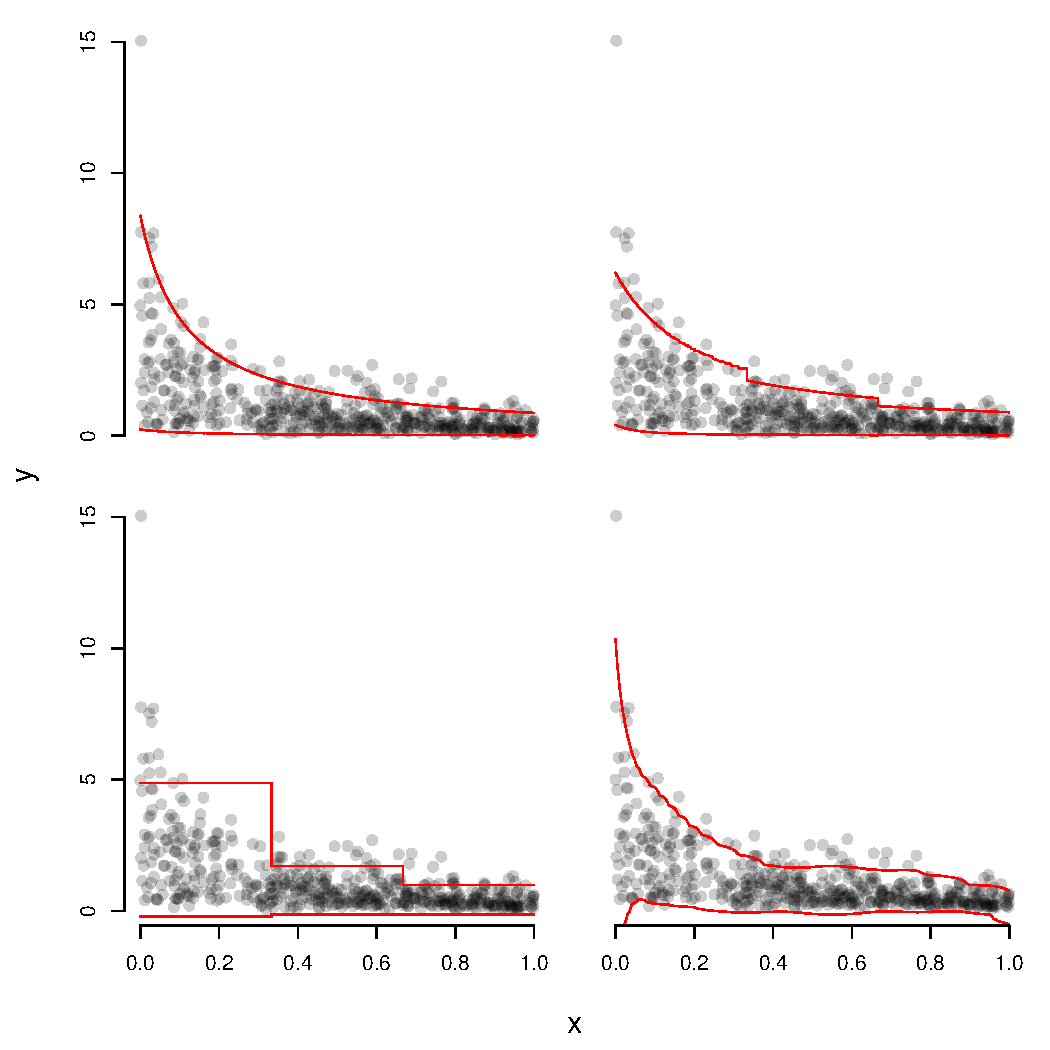
\includegraphics[width=\maxwidth]{figure/gammasimexample-1} 

\end{knitrout}
\end{center}
\caption{Sim setting: $n = 500$, shape = $2$, bins = $3$. 
  The regions are depicted as follows: 
    transformation based parametric conformal prediction (top-left panel),
    binned parametric conformal prediction region (top-right panel),
    nonparametric conformal prediction region (bottom-left panel), and 
    LSLW conformal prediction region (bottom-right panel).}
\label{Fig:plots}
\end{figure}

In Figure~\ref{Fig:plots2} we see that the transformation parametric conformal 
prediction region closely resembles the HD prediction region, and that the 
binned parametric conformal prediction region is a close descretization of 
the HD prediction region.


\begin{figure}[h!]
\begin{center}
\begin{knitrout}
\definecolor{shadecolor}{rgb}{0.969, 0.969, 0.969}\color{fgcolor}
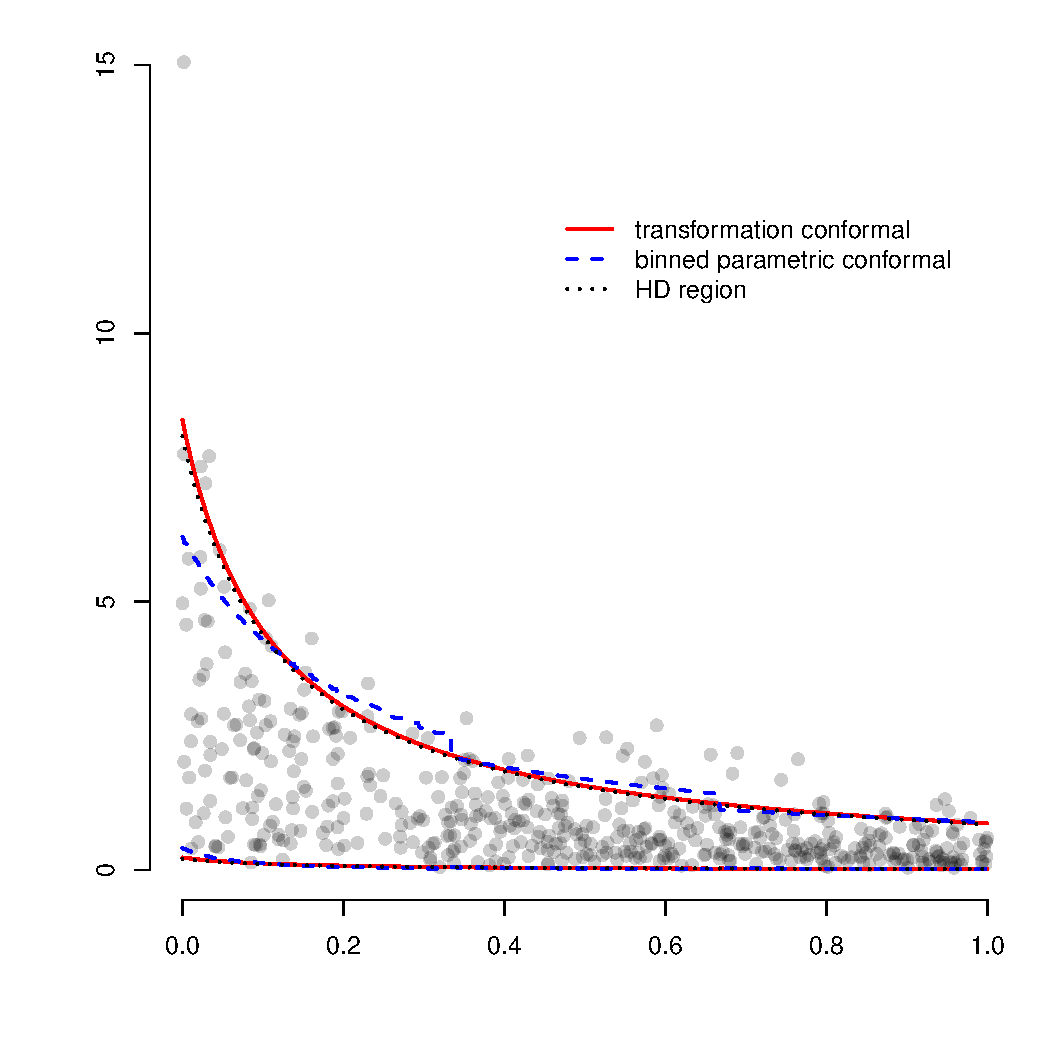
\includegraphics[width=\maxwidth]{figure/gammasimexample2-1} 

\end{knitrout}
\end{center}
\label{Fig:plots2}
\end{figure}


All of the presented prediction regions exhibit close to finite-sample 
marginal validity and local validity with respect to binning.  However, 
the transformation conformal prediction region, LSLW conformal prediction 
region, and the HD prediction region do not exhibit finite-sample local 
validity in the second bin and the HD prediction region does not quite 
possess finite-sample marginal validity.  
The binned parametric conformal prediction region is smallest in size 
with an estimated area of 2.19.  The HD prediction region is a close second 
with an estimated area of 2.21.  The tranformation conformal prediction 
region is a respectable third with an estimated area of 2.26.
LSLW conformal prediction region has an estimated area of 2.56 and 
The nonparametric conformal prediction region has an estimated area of 2.68. 
Under correct model specification, the parametric conformal prediction 
regions are similar in performance to that of the highest density prediction 
region.



\begin{knitrout}
\definecolor{shadecolor}{rgb}{0.969, 0.969, 0.969}\color{fgcolor}\begin{kframe}
\begin{alltt}
\hlcom{#########################################}
\hlcom{## area and coverage}

\hlcom{# nonparametric conformal prediction region}
\hlcom{# estimated area}
\hlstd{area.nonparametric} \hlkwb{<-} \hlkwa{function}\hlstd{(}\hlkwc{region}\hlstd{)\{}
  \hlkwa{if}\hlstd{(}\hlkwd{class}\hlstd{(region)} \hlopt{!=} \hlstr{"list"}\hlstd{)\{}
    \hlkwd{stop}\hlstd{(}\hlstr{"Only appropriate for nonparametric conformal prediction region"}\hlstd{)}
  \hlstd{\}}
  \hlstd{bins} \hlkwb{<-} \hlkwd{length}\hlstd{(region); wn} \hlkwb{<-} \hlnum{1} \hlopt{/} \hlstd{bins}
  \hlstd{area} \hlkwb{<-} \hlnum{0}
  \hlkwa{for}\hlstd{(i} \hlkwa{in} \hlnum{1}\hlopt{:}\hlstd{bins)\{}
    \hlstd{nonpar.region} \hlkwb{<-} \hlstd{region[[i]]}
    \hlstd{area} \hlkwb{<-} \hlstd{area} \hlopt{+} \hlstd{wn} \hlopt{*} \hlkwd{as.numeric}\hlstd{(}\hlkwd{rep}\hlstd{(}\hlkwd{c}\hlstd{(}\hlopt{-}\hlnum{1}\hlstd{,}\hlnum{1}\hlstd{),}
      \hlkwd{length}\hlstd{(nonpar.region)}\hlopt{/}\hlnum{2}\hlstd{)} \hlopt \hlstd{nonpar.region)}
  \hlstd{\}}
  \hlstd{area}
\hlstd{\}}
\hlcom{# estimated area of prediction regions}
\hlstd{area} \hlkwb{<-} \hlkwd{c}\hlstd{(}
  \hlkwd{mean}\hlstd{(}\hlkwd{apply}\hlstd{(transformCI,} \hlnum{1}\hlstd{, diff)),}
  \hlkwd{mean}\hlstd{(}\hlkwd{apply}\hlstd{(parabinCI,} \hlnum{1}\hlstd{, diff)),}
  \hlkwd{area.nonparametric}\hlstd{(nonparabinCI),}
  \hlkwd{mean}\hlstd{(}\hlkwd{apply}\hlstd{(LSLW,} \hlnum{1}\hlstd{, diff)),}
  \hlkwd{mean}\hlstd{(}\hlkwd{apply}\hlstd{(HDCI,} \hlnum{1}\hlstd{, diff))}
\hlstd{)}

\hlcom{# marginal local coverage of prediction regions}
\hlstd{p} \hlkwb{<-} \hlnum{1}
\hlstd{marginalcov} \hlkwb{<-} \hlkwd{c}\hlstd{(}
  \hlkwd{local.coverage}\hlstd{(}\hlkwc{region} \hlstd{= transformCI,} \hlkwc{data} \hlstd{= data.readme,} \hlkwc{d} \hlstd{= p,}
    \hlkwc{bins} \hlstd{=} \hlnum{1}\hlstd{,} \hlkwc{at.data} \hlstd{=} \hlstr{"TRUE"}\hlstd{),}
  \hlkwd{local.coverage}\hlstd{(}\hlkwc{region} \hlstd{= parabinCI,} \hlkwc{data} \hlstd{= data.readme,} \hlkwc{d} \hlstd{= p,}
    \hlkwc{bins} \hlstd{=} \hlnum{1}\hlstd{,} \hlkwc{at.data} \hlstd{=} \hlstr{"TRUE"}\hlstd{),}
  \hlkwd{local.coverage}\hlstd{(}\hlkwc{region} \hlstd{= nonparabinCI,} \hlkwc{data} \hlstd{= data.readme,} \hlkwc{d} \hlstd{= p,}
    \hlkwc{nonparametric} \hlstd{=} \hlstr{"TRUE"}\hlstd{,} \hlkwc{bins} \hlstd{=} \hlnum{1}\hlstd{,} \hlkwc{at.data} \hlstd{=} \hlstr{"TRUE"}\hlstd{),}
  \hlkwd{local.coverage}\hlstd{(}\hlkwc{region} \hlstd{= LSLW,} \hlkwc{data} \hlstd{= data.readme,} \hlkwc{d} \hlstd{= p,}
    \hlkwc{bins} \hlstd{=} \hlnum{1}\hlstd{,} \hlkwc{at.data} \hlstd{=} \hlstr{"TRUE"}\hlstd{),}
  \hlkwd{local.coverage}\hlstd{(}\hlkwc{region} \hlstd{= HDCI,} \hlkwc{data} \hlstd{= data.readme,} \hlkwc{d} \hlstd{= p,}
    \hlkwc{bins} \hlstd{=} \hlnum{1}\hlstd{,} \hlkwc{at.data} \hlstd{=} \hlstr{"TRUE"}\hlstd{)}
\hlstd{)}

\hlcom{# local coverage of prediction regions}
\hlstd{localcov} \hlkwb{<-} \hlkwd{cbind}\hlstd{(}
  \hlkwd{local.coverage}\hlstd{(}\hlkwc{region} \hlstd{= transformCI,} \hlkwc{data} \hlstd{= data.readme,} \hlkwc{d} \hlstd{= p,}
    \hlkwc{bins} \hlstd{= bins,} \hlkwc{at.data} \hlstd{=} \hlstr{"TRUE"}\hlstd{),}
  \hlkwd{local.coverage}\hlstd{(}\hlkwc{region} \hlstd{= parabinCI,} \hlkwc{data} \hlstd{= data.readme,} \hlkwc{d} \hlstd{= p,}
    \hlkwc{bins} \hlstd{= bins,} \hlkwc{at.data} \hlstd{=} \hlstr{"TRUE"}\hlstd{),}
  \hlkwd{local.coverage}\hlstd{(}\hlkwc{region} \hlstd{= nonparabinCI,} \hlkwc{data} \hlstd{= data.readme,} \hlkwc{d} \hlstd{= p,}
    \hlkwc{nonparametric} \hlstd{=} \hlstr{"TRUE"}\hlstd{,} \hlkwc{bins} \hlstd{= bins,} \hlkwc{at.data} \hlstd{=} \hlstr{"TRUE"}\hlstd{),}
  \hlkwd{local.coverage}\hlstd{(}\hlkwc{region} \hlstd{= LSLW,} \hlkwc{data} \hlstd{= data.readme,} \hlkwc{d} \hlstd{= p,}
    \hlkwc{bins} \hlstd{= bins,} \hlkwc{at.data} \hlstd{=} \hlstr{"TRUE"}\hlstd{),}
  \hlkwd{local.coverage}\hlstd{(}\hlkwc{region} \hlstd{= HDCI,} \hlkwc{data} \hlstd{= data.readme,} \hlkwc{d} \hlstd{= p,}
    \hlkwc{bins} \hlstd{= bins,} \hlkwc{at.data} \hlstd{=} \hlstr{"TRUE"}\hlstd{)}
\hlstd{)}

\hlcom{# diagnostics}
\hlstd{diagnostics} \hlkwb{<-} \hlkwd{rbind}\hlstd{(area, marginalcov, localcov)}
\hlkwd{colnames}\hlstd{(diagnostics)} \hlkwb{<-} \hlkwd{c}\hlstd{(}\hlstr{"transformCI"}\hlstd{,} \hlstr{"binparaCI"}\hlstd{,}
  \hlstr{"binnonparaCI"}\hlstd{,} \hlstr{"LSLW"}\hlstd{,} \hlstr{"HDCI"}\hlstd{)}
\hlkwd{rownames}\hlstd{(diagnostics)} \hlkwb{<-} \hlkwd{c}\hlstd{(}\hlstr{"area"}\hlstd{,} \hlstr{"marginal coverage"}\hlstd{,} \hlstr{"bin 1 coverage"}\hlstd{,}
  \hlstr{"bin 2 coverage"}\hlstd{,} \hlstr{"bin 3 coverage"}\hlstd{)}
\end{alltt}
\end{kframe}
\end{knitrout}


\begin{kframe}
\begin{alltt}
\hlkwd{xtable}\hlstd{(diagnostics,} \hlkwc{digits} \hlstd{=} \hlkwd{c}\hlstd{(}\hlnum{0}\hlstd{,} \hlnum{2}\hlstd{,} \hlnum{2}\hlstd{,} \hlnum{2}\hlstd{,} \hlnum{2}\hlstd{,} \hlnum{2}\hlstd{))}
\end{alltt}
\end{kframe}% latex table generated in R 3.4.4 by xtable 1.8-3 package
% Mon Oct  7 13:40:01 2019
\begin{table}[ht]
\centering
\begin{tabular}{rrrrrr}
  \hline
 & transformCI & binparaCI & binnonparaCI & LSLW & HDCI \\ 
  \hline
area & 2.26 & 2.19 & 2.68 & 2.02 & 2.21 \\ 
  marginal coverage & 0.91 & 0.91 & 0.91 & 0.77 & 0.90 \\ 
  bin 1 coverage & 0.91 & 0.91 & 0.93 & 0.81 & 0.90 \\ 
  bin 2 coverage & 0.89 & 0.90 & 0.90 & 0.75 & 0.88 \\ 
  bin 3 coverage & 0.93 & 0.91 & 0.90 & 0.74 & 0.91 \\ 
   \hline
\end{tabular}
\end{table}



\section{Extension of the illustrative example from the README file}

In this extension we investigate the local coverage properties of six  
prediction regions, the five from the previous section and a least squares 
(LS) conformal prediction region without local weighting.  Local coverage is 
assessed via a Monte Carlo simulation of size $B = 50$.  At each iteration 
of this simulation a new dataset is generated under the same specifications 
as those in the README file.  We then compute the local coverage probabilities 
with respect to each bin and also approximate conditional coverage across $x$.  
We do not assess coverage properties directly at $x$ for all $x \in (0,1]$.  
This corresponds to the notion of conditional validity which cannot be 
achieved in tandem with an oracle estimation in finite sample settings when 
distributions are continuous \citep[Section 2.2]{lei2014distribution}.  
What we do instead is we assess local coverage with a binning in $x$ that is 
much finer than the binning that was used to create the misspecified 
parametric and nonparametric conformal prediction regions.  We form 25 bins 
of length 0.04. 



\subsection{Diagnostic measures}

Several diagnostic measures are used to compare conformal prediction regions.
These diagnostic measures compare prediction regions by their 
prediction error, volume, and coverage properties.
Our prediction error diagnostic metric will be an average of the squared 
distances of observations outside of the prediction region to the closest 
boundary of the prediction region, averaged over all 
observations. An observation that falls within the prediction region 
has an error of 0.  More formally this prediction error metric is 
$$
  \text{prediction error} 
    = n^{-1}\sum_{i=1}^n\indicator{Y_i \not\in \Copt(X_i)}
      \left(\min_{j=1,\ldots,m_i}\left\{\min\{|Y_i - a_{i,j}|, 
        |Y_i - b_{i,j}|\}\right\}\right)^2,
$$
where $a_{i,j}$ and $b_{i,j}$ are, respectively, the lower and upper 
boundaries of possible $j = 1, \ldots, m_i$ disjoint intervals forming 
the prediction region.  

The volume of each prediction region will be estimated by the average of the 
upper boundary minus the lower boundary across observed $\X$, written as
$$ 
  \text{area} = n^{-1}\sum_{i=1}^n\sum_{j=1}^{m_i}(b_{i,j} - a_{i,j}).
$$
%This estimate of area is appropriate in our simulations in which realizations 
%of the predictors are generated as $X \sim U(0,1)$.   

%The area of each prediction region will be estimated by the average of the 
%upper boundary minus the lower boundary across observed $\X$, written as
%$$ 
%  \text{area} = n^{-1}\sum_{i=1}^n\sum_{j=1}^{m_i}(b_{i,j} - a_{i,j}).
%$$
%This estimate of area is appropriate in our simulations in which realiztions 
%of the predictors are generated as $X \sim U(0,1)$.   

To assess finite-sample marginal validity we calculate the proportion of 
responses that fall within the prediction region.  To assess finite-sample 
local validity with respect to binning we first bin the predictor data and 
then, for each bin, we calculate the proportion of responses that fall 
within the prediction region. The same procedure is used to assess 
finite-sample conditional validity, but we use a much finer binning regime 
than what was used to assess finite-sample local validity.  

The following function computes our estimate of prediction error at the 
observed data when the prediction region is not the nonparametric 
conformal prediction region.

\begin{knitrout}
\definecolor{shadecolor}{rgb}{0.969, 0.969, 0.969}\color{fgcolor}\begin{kframe}
\begin{alltt}
\hlstd{absolute.error} \hlkwb{<-} \hlkwa{function}\hlstd{(}\hlkwc{y}\hlstd{,} \hlkwc{region}\hlstd{,} \hlkwc{squared} \hlstd{=} \hlnum{TRUE}\hlstd{)\{}
  \hlstd{lwr} \hlkwb{<-} \hlstd{region[,} \hlnum{1}\hlstd{]}
  \hlstd{upr} \hlkwb{<-} \hlstd{region[,} \hlnum{2}\hlstd{]}
  \hlstd{index} \hlkwb{<-} \hlkwd{which}\hlstd{(}\hlopt{!}\hlstd{(lwr} \hlopt{<=} \hlstd{y} \hlopt{&} \hlstd{y} \hlopt{<=} \hlstd{upr))}
  \hlstd{out} \hlkwb{<-} \hlkwd{sum}\hlstd{(}\hlkwd{unlist}\hlstd{(}\hlkwd{lapply}\hlstd{(index,} \hlkwa{function}\hlstd{(}\hlkwc{j}\hlstd{)\{}
    \hlstd{error} \hlkwb{<-} \hlkwa{NULL}
    \hlkwa{if}\hlstd{(squared} \hlopt{==} \hlnum{FALSE}\hlstd{) error} \hlkwb{<-}
      \hlkwd{min}\hlstd{(}\hlkwd{abs}\hlstd{(y[j]} \hlopt{-} \hlstd{lwr[j]),} \hlkwd{abs}\hlstd{(y[j]} \hlopt{-} \hlstd{upr[j]))}
    \hlkwa{if}\hlstd{(squared} \hlopt{==} \hlnum{TRUE}\hlstd{) error} \hlkwb{<-}
      \hlstd{(}\hlkwd{min}\hlstd{(}\hlkwd{abs}\hlstd{(y[j]} \hlopt{-} \hlstd{lwr[j]),} \hlkwd{abs}\hlstd{(y[j]} \hlopt{-} \hlstd{upr[j])))}\hlopt{^}\hlnum{2}
    \hlstd{error}
  \hlstd{\})))} \hlopt{/} \hlkwd{length}\hlstd{(y)}
  \hlstd{out}
\hlstd{\}}
\end{alltt}
\end{kframe}
\end{knitrout}

The following function computes our estimate of prediction error at the 
observed data when the prediction region is the nonparametric conformal 
prediction region.

\begin{knitrout}
\definecolor{shadecolor}{rgb}{0.969, 0.969, 0.969}\color{fgcolor}\begin{kframe}
\begin{alltt}
\hlstd{absolute.error.nonparametric} \hlkwb{<-} \hlkwa{function}\hlstd{(}\hlkwc{data}\hlstd{,} \hlkwc{region}\hlstd{,}
  \hlkwc{squared} \hlstd{=} \hlnum{TRUE}\hlstd{)\{}
  \hlstd{n} \hlkwb{<-} \hlkwd{nrow}\hlstd{(data)}
  \hlstd{n.bins.region} \hlkwb{<-} \hlkwd{length}\hlstd{(region)}
  \hlstd{d} \hlkwb{<-} \hlkwd{ncol}\hlstd{(data)} \hlopt{-} \hlnum{1}
  \hlstd{x} \hlkwb{<-} \hlkwd{as.matrix}\hlstd{(data[,}\hlnum{1}\hlopt{:}\hlstd{d} \hlopt{+} \hlnum{1}\hlstd{],} \hlkwc{col} \hlstd{= d)}
  \hlstd{index.bins.region} \hlkwb{<-} \hlkwd{find.index}\hlstd{(x,} \hlkwc{wn} \hlstd{=} \hlnum{1}\hlopt{/}\hlstd{n.bins.region,} \hlkwc{d} \hlstd{= d)}
  \hlstd{y} \hlkwb{<-} \hlstd{data[,} \hlnum{1}\hlstd{]}
  \hlstd{area} \hlkwb{<-} \hlnum{0}
  \hlkwa{for}\hlstd{(j} \hlkwa{in} \hlnum{1}\hlopt{:}\hlstd{n)\{}
    \hlstd{index.j} \hlkwb{<-} \hlkwd{which}\hlstd{(index.bins.region} \hlopt{==} \hlstd{j)}
    \hlstd{error} \hlkwb{<-} \hlkwd{c}\hlstd{(y[j]} \hlopt{-} \hlstd{region[[index.bins.region[j]]])}
    \hlstd{index} \hlkwb{<-} \hlnum{0}
    \hlkwa{if}\hlstd{(}\hlkwd{any}\hlstd{(error} \hlopt{>} \hlnum{0}\hlstd{)) index} \hlkwb{<-} \hlkwd{max}\hlstd{(}\hlkwd{which}\hlstd{(error} \hlopt{>} \hlnum{0}\hlstd{))}
    \hlkwa{if}\hlstd{(index} \hlopt \hlnum{2} \hlopt{==} \hlnum{0}\hlstd{)\{}
      \hlkwa{if}\hlstd{(squared} \hlopt{==} \hlnum{FALSE}\hlstd{) area} \hlkwb{<-}
        \hlstd{area} \hlopt{+} \hlkwd{min}\hlstd{(}\hlkwd{abs}\hlstd{(error))} \hlopt{/} \hlstd{n}
      \hlkwa{if}\hlstd{(squared} \hlopt{==} \hlnum{TRUE}\hlstd{) area} \hlkwb{<-}
        \hlstd{area} \hlopt{+} \hlkwd{min}\hlstd{(}\hlkwd{abs}\hlstd{(error))}\hlopt{^}\hlnum{2} \hlopt{/} \hlstd{n}
    \hlstd{\}}
  \hlstd{\}}
  \hlstd{area}
\hlstd{\}}
\end{alltt}
\end{kframe}
\end{knitrout}

Our Monte Carlo simulator follows. This function computes all of the 
dignostics and local coverage probabilities for each prediction region 
for every generated dataset.


\begin{knitrout}
\definecolor{shadecolor}{rgb}{0.969, 0.969, 0.969}\color{fgcolor}\begin{kframe}
\begin{alltt}
\hlstd{dat} \hlkwb{<-} \hlkwd{data.frame}\hlstd{(}\hlkwc{y} \hlstd{= y,} \hlkwc{x1} \hlstd{= x)}
\hlstd{gamma_simulator} \hlkwb{<-} \hlkwa{function}\hlstd{(}\hlkwc{beta}\hlstd{,} \hlkwc{n} \hlstd{=} \hlnum{500}\hlstd{,} \hlkwc{alpha} \hlstd{=} \hlnum{0.10}\hlstd{,} \hlkwc{bins} \hlstd{=} \hlnum{3}\hlstd{,}
  \hlkwc{family} \hlstd{=} \hlstr{"Gamma"}\hlstd{,} \hlkwc{link} \hlstd{=} \hlstr{"inverse"}\hlstd{,} \hlkwc{shape} \hlstd{=} \hlnum{2}\hlstd{,}
  \hlkwc{parametric} \hlstd{=} \hlnum{TRUE}\hlstd{,} \hlkwc{nonparametric} \hlstd{=} \hlnum{TRUE}\hlstd{,} \hlkwc{method} \hlstd{=} \hlstr{"both"}\hlstd{,}
  \hlkwc{LS} \hlstd{=} \hlnum{TRUE}\hlstd{,} \hlkwc{LSLW} \hlstd{=} \hlnum{TRUE}\hlstd{,} \hlkwc{HD} \hlstd{=} \hlnum{TRUE}\hlstd{,} \hlkwc{cores} \hlstd{=} \hlnum{7}\hlstd{)\{}

  \hlcom{## in this univariate problem, p and d are the same}
  \hlstd{p} \hlkwb{<-} \hlstd{d} \hlkwb{<-} \hlkwd{length}\hlstd{(beta)} \hlopt{-} \hlnum{1}
  \hlstd{x} \hlkwb{<-} \hlkwd{matrix}\hlstd{(}\hlkwd{runif}\hlstd{(n}\hlopt{*}\hlstd{p),} \hlkwc{ncol} \hlstd{= p)}
  \hlstd{y} \hlkwb{<-} \hlkwd{rep}\hlstd{(}\hlnum{0}\hlstd{,n)}
  \hlstd{dat} \hlkwb{<-} \hlkwd{data.frame}\hlstd{(}\hlkwc{y} \hlstd{= y,} \hlkwc{x} \hlstd{= x)}
  \hlkwd{colnames}\hlstd{(dat)[}\hlnum{2}\hlopt{:}\hlstd{(p}\hlopt{+}\hlnum{1}\hlstd{)]} \hlkwb{<-} \hlkwd{paste}\hlstd{(}\hlstr{"x"}\hlstd{,} \hlnum{1}\hlopt{:}\hlstd{p,} \hlkwc{sep} \hlstd{=} \hlstr{""}\hlstd{)}

  \hlcom{## set up partition}
  \hlkwa{if}\hlstd{(}\hlkwd{class}\hlstd{(bins)} \hlopt{==} \hlstr{"NULL"}\hlstd{)\{}
    \hlstd{wn} \hlkwb{<-} \hlkwd{min}\hlstd{(}\hlnum{1}\hlopt{/} \hlkwd{floor}\hlstd{(}\hlnum{1} \hlopt{/} \hlstd{(}\hlkwd{log}\hlstd{(n)}\hlopt{/}\hlstd{n)}\hlopt{^}\hlstd{(}\hlnum{1}\hlopt{/}\hlstd{(d}\hlopt{+}\hlnum{3}\hlstd{))),} \hlnum{1}\hlopt{/}\hlnum{2}\hlstd{)}
    \hlstd{bins} \hlkwb{<-} \hlnum{1} \hlopt{/} \hlstd{wn}
  \hlstd{\}}

  \hlcom{## generate the data (has functionality for different }
  \hlcom{## families and link functions)}
  \hlkwa{if}\hlstd{(family} \hlopt{==} \hlstr{"Gamma"}\hlstd{)\{}
    \hlkwa{if}\hlstd{(link} \hlopt{==} \hlstr{"identity"}\hlstd{)\{}
      \hlstd{rate} \hlkwb{<-} \hlstd{(}\hlnum{1} \hlopt{/} \hlstd{(}\hlkwd{cbind}\hlstd{(}\hlnum{1}\hlstd{, x)} \hlopt \hlstd{beta))} \hlopt{*} \hlstd{shape}
      \hlstd{y} \hlkwb{<-} \hlkwd{rgamma}\hlstd{(}\hlkwc{n} \hlstd{= n,} \hlkwc{shape} \hlstd{= shape,} \hlkwc{rate} \hlstd{= rate)}
      \hlstd{dat}\hlopt{$}\hlstd{y} \hlkwb{<-} \hlstd{y} \hlopt{/} \hlkwd{sd}\hlstd{(y)}
    \hlstd{\}}
    \hlkwa{if}\hlstd{(link} \hlopt{==} \hlstr{"inverse"}\hlstd{)\{}
      \hlstd{rate} \hlkwb{<-} \hlstd{(}\hlkwd{cbind}\hlstd{(}\hlnum{1}\hlstd{, x)} \hlopt \hlstd{beta)} \hlopt{*} \hlstd{shape}
      \hlstd{y} \hlkwb{<-} \hlkwd{rgamma}\hlstd{(}\hlkwc{n} \hlstd{= n,} \hlkwc{shape} \hlstd{= shape,} \hlkwc{rate} \hlstd{= rate)}
      \hlstd{dat}\hlopt{$}\hlstd{y} \hlkwb{<-} \hlstd{y} \hlopt{/} \hlkwd{sd}\hlstd{(y)}
    \hlstd{\}}
    \hlkwa{if}\hlstd{(link} \hlopt{==} \hlstr{"log"}\hlstd{)\{}
      \hlstd{rate} \hlkwb{<-} \hlstd{(}\hlnum{1} \hlopt{/} \hlkwd{exp}\hlstd{(}\hlkwd{cbind}\hlstd{(}\hlnum{1}\hlstd{, x)} \hlopt \hlstd{beta))} \hlopt{*} \hlstd{shape}
      \hlstd{y} \hlkwb{<-} \hlkwd{rgamma}\hlstd{(}\hlkwc{n} \hlstd{= n,} \hlkwc{shape} \hlstd{= shape,} \hlkwc{rate} \hlstd{= rate)}
      \hlstd{dat}\hlopt{$}\hlstd{y} \hlkwb{<-} \hlstd{y} \hlopt{/} \hlkwd{sd}\hlstd{(y)}
    \hlstd{\}}
  \hlstd{\}}
  \hlkwa{if}\hlstd{(family} \hlopt{==} \hlstr{"gaussian"}\hlstd{)\{}
    \hlstd{mu} \hlkwb{<-} \hlkwd{cbind}\hlstd{(}\hlnum{1}\hlstd{, x)} \hlopt \hlstd{beta}
    \hlstd{y} \hlkwb{<-} \hlkwd{rnorm}\hlstd{(}\hlkwc{n} \hlstd{= n,} \hlkwc{mean} \hlstd{= mu,} \hlkwc{sd} \hlstd{= sd)}
    \hlstd{dat}\hlopt{$}\hlstd{y} \hlkwb{<-} \hlstd{y} \hlopt{/} \hlkwd{sd}\hlstd{(y)}
  \hlstd{\}}
  \hlkwa{if}\hlstd{(family} \hlopt{==} \hlstr{"inverse.gaussian"}\hlstd{)\{}
    \hlstd{mu} \hlkwb{=} \hlnum{1} \hlopt{/} \hlkwd{sqrt}\hlstd{(}\hlkwd{cbind}\hlstd{(}\hlnum{1}\hlstd{, x)} \hlopt \hlstd{beta)}
    \hlstd{y} \hlkwb{<-} \hlkwd{rinvgauss}\hlstd{(}\hlkwc{n} \hlstd{= n,} \hlkwc{mean} \hlstd{= mu)}
    \hlstd{dat}\hlopt{$}\hlstd{y} \hlkwb{<-} \hlstd{y} \hlopt{/} \hlkwd{sd}\hlstd{(y)}
  \hlstd{\}}

  \hlcom{## fit the Gamma regression model}
  \hlstd{fit} \hlkwb{<-} \hlkwd{glm}\hlstd{(y} \hlopt{~} \hlstd{x1,} \hlkwc{family} \hlstd{=} \hlstr{"Gamma"}\hlstd{,} \hlkwc{data} \hlstd{= dat)}
  \hlstd{parabinCI} \hlkwb{<-} \hlstd{transformCI} \hlkwb{<-} \hlstd{nonparabinCI} \hlkwb{<-} \hlstd{LSCI} \hlkwb{<-}
    \hlstd{LSLWCI} \hlkwb{<-} \hlstd{HDCI} \hlkwb{<-} \hlkwa{NULL}
  \hlstd{formula} \hlkwb{<-} \hlstd{fit}\hlopt{$}\hlstd{formula}
  \hlstd{newdata} \hlkwb{<-} \hlstd{dat}
  \hlstd{respname} \hlkwb{<-} \hlkwd{all.vars}\hlstd{(formula)[}\hlnum{1}\hlstd{]}
  \hlstd{newdata} \hlkwb{<-} \hlstd{newdata[,} \hlopt{!}\hlstd{(}\hlkwd{colnames}\hlstd{(dat)} \hlopt \hlstd{respname)]}
  \hlstd{newdata} \hlkwb{<-} \hlkwd{as.matrix}\hlstd{(newdata)}

  \hlcom{## obtain the prediction regions}
  \hlstd{output.parabin} \hlkwb{<-} \hlstd{output.transform} \hlkwb{<-} \hlstd{output.nonparabin} \hlkwb{<-}
    \hlstd{output.LS} \hlkwb{<-} \hlstd{output.LSLW} \hlkwb{<-} \hlstd{output.HD} \hlkwb{<-} \hlkwd{rep}\hlstd{(}\hlnum{NA}\hlstd{, bins} \hlopt{+} \hlnum{1}\hlstd{)}
  \hlkwa{if}\hlstd{(parametric)\{}
    \hlstd{cpred} \hlkwb{<-} \hlkwd{conformal.glm}\hlstd{(fit,} \hlkwc{parametric} \hlstd{=} \hlnum{TRUE}\hlstd{,}
      \hlkwc{nonparametric} \hlstd{=} \hlnum{FALSE}\hlstd{,} \hlkwc{alpha} \hlstd{= alpha,} \hlkwc{method} \hlstd{=} \hlstr{"both"}\hlstd{,}
      \hlkwc{bins} \hlstd{= bins,} \hlkwc{cores} \hlstd{= cores,} \hlkwc{newdata} \hlstd{= newdata,}
      \hlkwc{precision} \hlstd{=} \hlnum{0.02}\hlstd{)}

    \hlcom{# bin parametric conformal}
    \hlstd{parabinCI} \hlkwb{<-} \hlstd{cpred}\hlopt{$}\hlstd{paraconfbin}
    \hlstd{marginal.parabin} \hlkwb{<-} \hlkwd{local.coverage}\hlstd{(}\hlkwc{region} \hlstd{= parabinCI,}
      \hlkwc{data} \hlstd{= dat,} \hlkwc{d} \hlstd{= p,} \hlkwc{bins} \hlstd{=} \hlnum{1}\hlstd{,} \hlkwc{at.data} \hlstd{=} \hlstr{"TRUE"}\hlstd{)}
    \hlstd{local.parabin} \hlkwb{<-} \hlkwd{local.coverage}\hlstd{(}\hlkwc{region} \hlstd{= parabinCI,}
      \hlkwc{data} \hlstd{= dat,} \hlkwc{d} \hlstd{= p,} \hlkwc{bins} \hlstd{= bins,} \hlkwc{at.data} \hlstd{=} \hlstr{"TRUE"}\hlstd{)}
    \hlstd{local.inx.parabin} \hlkwb{<-} \hlkwd{local.coverage}\hlstd{(}\hlkwc{region} \hlstd{= parabinCI,}
      \hlkwc{data} \hlstd{= dat,} \hlkwc{d} \hlstd{= p,} \hlkwc{bins} \hlstd{=} \hlnum{25}\hlstd{,} \hlkwc{at.data} \hlstd{=} \hlstr{"TRUE"}\hlstd{)}
    \hlstd{output.parabin} \hlkwb{<-} \hlkwd{c}\hlstd{(marginal.parabin, local.parabin,}
      \hlstd{local.inx.parabin,}
      \hlkwd{mean}\hlstd{(}\hlkwd{apply}\hlstd{(parabinCI,} \hlnum{1}\hlstd{, diff)),}
      \hlkwd{absolute.error}\hlstd{(}\hlkwc{y} \hlstd{= y,} \hlkwc{region} \hlstd{= parabinCI))}

    \hlcom{# transform parametric conformal}
    \hlstd{transformCI} \hlkwb{<-} \hlstd{cpred}\hlopt{$}\hlstd{transformconf}
    \hlstd{marginal.transform} \hlkwb{<-} \hlkwd{local.coverage}\hlstd{(}\hlkwc{region} \hlstd{= transformCI,}
      \hlkwc{data} \hlstd{= dat,} \hlkwc{d} \hlstd{= p,} \hlkwc{bins} \hlstd{=} \hlnum{1}\hlstd{,} \hlkwc{at.data} \hlstd{=} \hlstr{"TRUE"}\hlstd{)}
    \hlstd{local.transform} \hlkwb{<-} \hlkwd{local.coverage}\hlstd{(}\hlkwc{region} \hlstd{= transformCI,}
      \hlkwc{data} \hlstd{= dat,} \hlkwc{d} \hlstd{= p,} \hlkwc{bins} \hlstd{= bins,} \hlkwc{at.data} \hlstd{=} \hlstr{"TRUE"}\hlstd{)}
    \hlstd{local.inx.transform} \hlkwb{<-} \hlkwd{local.coverage}\hlstd{(}\hlkwc{region} \hlstd{= transformCI,}
      \hlkwc{data} \hlstd{= dat,} \hlkwc{d} \hlstd{= p,} \hlkwc{bins} \hlstd{=} \hlnum{25}\hlstd{,} \hlkwc{at.data} \hlstd{=} \hlstr{"TRUE"}\hlstd{)}
    \hlstd{output.transform} \hlkwb{<-} \hlkwd{c}\hlstd{(marginal.transform, local.transform,}
      \hlstd{local.inx.transform,}
      \hlkwd{mean}\hlstd{(}\hlkwd{apply}\hlstd{(transformCI,} \hlnum{1}\hlstd{, diff)),}
      \hlkwd{absolute.error}\hlstd{(}\hlkwc{y} \hlstd{= y,} \hlkwc{region} \hlstd{= transformCI))}
  \hlstd{\}}
  \hlkwa{if}\hlstd{(nonparametric)\{}
    \hlstd{cpred} \hlkwb{<-} \hlkwd{conformal.glm}\hlstd{(fit,} \hlkwc{parametric} \hlstd{=} \hlnum{FALSE}\hlstd{,}
      \hlkwc{nonparametric} \hlstd{=} \hlnum{TRUE}\hlstd{,} \hlkwc{alpha} \hlstd{= alpha,} \hlkwc{method} \hlstd{=} \hlstr{"both"}\hlstd{,}
      \hlkwc{bins} \hlstd{= bins,} \hlkwc{cores} \hlstd{= cores,} \hlkwc{precision} \hlstd{=} \hlnum{0.02}\hlstd{)}
    \hlstd{nonparabinCI} \hlkwb{<-} \hlstd{cpred}\hlopt{$}\hlstd{nonparaconfbin}

    \hlstd{marginal.nonparabin} \hlkwb{<-} \hlkwd{local.coverage}\hlstd{(}\hlkwc{region} \hlstd{= nonparabinCI,}
      \hlkwc{nonparametric} \hlstd{=} \hlstr{"TRUE"}\hlstd{,} \hlkwc{data} \hlstd{= dat,} \hlkwc{d} \hlstd{= p,} \hlkwc{bins} \hlstd{=} \hlnum{1}\hlstd{,}
      \hlkwc{at.data} \hlstd{=} \hlstr{"TRUE"}\hlstd{)}
    \hlstd{local.nonparabin} \hlkwb{<-} \hlkwd{local.coverage}\hlstd{(}\hlkwc{region} \hlstd{= nonparabinCI,}
      \hlkwc{nonparametric} \hlstd{=} \hlstr{"TRUE"}\hlstd{,} \hlkwc{data} \hlstd{= dat,} \hlkwc{d} \hlstd{= p,} \hlkwc{bins} \hlstd{= bins,}
      \hlkwc{at.data} \hlstd{=} \hlstr{"TRUE"}\hlstd{)}
    \hlstd{local.inx.nonparabin} \hlkwb{<-} \hlkwd{local.coverage}\hlstd{(}\hlkwc{region} \hlstd{= nonparabinCI,}
      \hlkwc{nonparametric} \hlstd{=} \hlstr{"TRUE"}\hlstd{,} \hlkwc{data} \hlstd{= dat,} \hlkwc{d} \hlstd{= p,} \hlkwc{bins} \hlstd{=} \hlnum{25}\hlstd{,}
      \hlkwc{at.data} \hlstd{=} \hlstr{"TRUE"}\hlstd{)}
    \hlstd{output.nonparabin} \hlkwb{<-}
      \hlkwd{c}\hlstd{(marginal.nonparabin, local.nonparabin,}
        \hlstd{local.inx.nonparabin,}
        \hlkwd{area.nonparametric}\hlstd{(nonparabinCI),}
        \hlkwd{absolute.error.nonparametric}\hlstd{(}\hlkwc{data} \hlstd{= dat,}
          \hlkwc{region} \hlstd{= nonparabinCI))}
  \hlstd{\}}
  \hlkwa{if}\hlstd{(LS)\{}
    \hlstd{p1.tibs} \hlkwb{<-} \hlkwd{conformal.pred}\hlstd{(}\hlkwc{x} \hlstd{=} \hlkwd{cbind}\hlstd{(x,x}\hlopt{^}\hlnum{2}\hlstd{,x}\hlopt{^}\hlnum{3}\hlstd{),} \hlkwc{y} \hlstd{= y,}
      \hlkwc{x0} \hlstd{=} \hlkwd{cbind}\hlstd{(x,x}\hlopt{^}\hlnum{2}\hlstd{,x}\hlopt{^}\hlnum{3}\hlstd{),}
      \hlkwc{train.fun} \hlstd{= train.fun,} \hlkwc{predict.fun} \hlstd{= predict.fun,}
      \hlkwc{alpha} \hlstd{= alpha)}
    \hlstd{LSCI} \hlkwb{<-} \hlkwd{cbind}\hlstd{(p1.tibs}\hlopt{$}\hlstd{lo, p1.tibs}\hlopt{$}\hlstd{up)}

    \hlstd{marginal.LS} \hlkwb{<-} \hlkwd{local.coverage}\hlstd{(}\hlkwc{region} \hlstd{= LSCI,}
      \hlkwc{data} \hlstd{= dat,} \hlkwc{d} \hlstd{= p,} \hlkwc{bins} \hlstd{=} \hlnum{1}\hlstd{,} \hlkwc{at.data} \hlstd{=} \hlstr{"TRUE"}\hlstd{)}
    \hlstd{local.LS} \hlkwb{<-} \hlkwd{local.coverage}\hlstd{(}\hlkwc{region} \hlstd{= LSCI,}
      \hlkwc{data} \hlstd{= dat,} \hlkwc{d} \hlstd{= p,} \hlkwc{bins} \hlstd{= bins,} \hlkwc{at.data} \hlstd{=} \hlstr{"TRUE"}\hlstd{)}
    \hlstd{local.inx.LS} \hlkwb{<-} \hlkwd{local.coverage}\hlstd{(}\hlkwc{region} \hlstd{= LSCI,}
      \hlkwc{data} \hlstd{= dat,} \hlkwc{d} \hlstd{= p,} \hlkwc{bins} \hlstd{=} \hlnum{25}\hlstd{,} \hlkwc{at.data} \hlstd{=} \hlstr{"TRUE"}\hlstd{)}
    \hlstd{output.LS} \hlkwb{<-} \hlkwd{c}\hlstd{(marginal.LS, local.LS, local.inx.LS,}
      \hlkwd{mean}\hlstd{(}\hlkwd{apply}\hlstd{(LSCI,} \hlnum{1}\hlstd{, diff)),}
      \hlkwd{absolute.error}\hlstd{(}\hlkwc{y} \hlstd{= y,} \hlkwc{region} \hlstd{= LSCI))}
  \hlstd{\}}
  \hlkwa{if}\hlstd{(LSLW)\{}
    \hlstd{cubic.model} \hlkwb{<-} \hlkwd{lm}\hlstd{(y} \hlopt{~} \hlstd{x} \hlopt{+} \hlkwd{I}\hlstd{(x}\hlopt{^}\hlnum{2}\hlstd{)} \hlopt{+} \hlkwd{I}\hlstd{(x}\hlopt{^}\hlnum{3}\hlstd{))}
    \hlstd{abs.resid} \hlkwb{<-} \hlkwd{abs}\hlstd{(cubic.model}\hlopt{$}\hlstd{resid)}
    \hlstd{smooth.call} \hlkwb{<-} \hlkwd{smooth.spline}\hlstd{(x, abs.resid,}
      \hlkwc{nknots} \hlstd{=} \hlnum{10}\hlstd{)}
    \hlstd{lambda} \hlkwb{<-} \hlstd{smooth.call}\hlopt{$}\hlstd{lambda}
    \hlstd{df} \hlkwb{<-} \hlstd{smooth.call}\hlopt{$}\hlstd{df}
    \hlstd{mad.train.fun} \hlkwb{<-} \hlkwa{function}\hlstd{(}\hlkwc{x}\hlstd{,} \hlkwc{y}\hlstd{,} \hlkwc{out} \hlstd{=} \hlkwa{NULL}\hlstd{)\{}
      \hlkwd{smooth.spline}\hlstd{(x[,} \hlnum{1}\hlstd{], y,} \hlkwc{lambda} \hlstd{= lambda,}
      \hlkwc{df} \hlstd{= df,} \hlkwc{nknots} \hlstd{=} \hlnum{10}\hlstd{)}
    \hlstd{\}}
    \hlstd{p2.tibs} \hlkwb{<-} \hlkwd{conformal.pred}\hlstd{(}\hlkwc{x} \hlstd{=} \hlkwd{cbind}\hlstd{(x,x}\hlopt{^}\hlnum{2}\hlstd{,x}\hlopt{^}\hlnum{3}\hlstd{),} \hlkwc{y} \hlstd{= y,}
      \hlkwc{x0} \hlstd{=} \hlkwd{cbind}\hlstd{(x,x}\hlopt{^}\hlnum{2}\hlstd{,x}\hlopt{^}\hlnum{3}\hlstd{),}
      \hlkwc{train.fun} \hlstd{= train.fun,} \hlkwc{predict.fun} \hlstd{= predict.fun,}
      \hlkwc{mad.train.fun} \hlstd{= mad.train.fun,}
      \hlkwc{mad.predict.fun} \hlstd{= mad.predict.fun,}
      \hlkwc{alpha} \hlstd{= alpha)}
    \hlstd{LSLWCI} \hlkwb{<-} \hlkwd{cbind}\hlstd{(p2.tibs}\hlopt{$}\hlstd{lo, p2.tibs}\hlopt{$}\hlstd{up)}

    \hlstd{marginal.LSLW} \hlkwb{<-} \hlkwd{local.coverage}\hlstd{(}\hlkwc{region} \hlstd{= LSLWCI,}
      \hlkwc{data} \hlstd{= dat,} \hlkwc{d} \hlstd{= p,} \hlkwc{bins} \hlstd{=} \hlnum{1}\hlstd{,} \hlkwc{at.data} \hlstd{=} \hlstr{"TRUE"}\hlstd{)}
    \hlstd{local.LSLW} \hlkwb{<-} \hlkwd{local.coverage}\hlstd{(}\hlkwc{region} \hlstd{= LSLWCI,}
      \hlkwc{data} \hlstd{= dat,} \hlkwc{d} \hlstd{= p,} \hlkwc{bins} \hlstd{= bins,} \hlkwc{at.data} \hlstd{=} \hlstr{"TRUE"}\hlstd{)}
    \hlstd{local.inx.LSLW} \hlkwb{<-} \hlkwd{local.coverage}\hlstd{(}\hlkwc{region} \hlstd{= LSLWCI,}
      \hlkwc{data} \hlstd{= dat,} \hlkwc{d} \hlstd{= p,} \hlkwc{bins} \hlstd{=} \hlnum{25}\hlstd{,} \hlkwc{at.data} \hlstd{=} \hlstr{"TRUE"}\hlstd{)}
    \hlstd{output.LSLW} \hlkwb{<-} \hlkwd{c}\hlstd{(marginal.LSLW, local.LSLW, local.inx.LSLW,}
      \hlkwd{mean}\hlstd{(}\hlkwd{apply}\hlstd{(LSLWCI,} \hlnum{1}\hlstd{, diff)),}
      \hlkwd{absolute.error}\hlstd{(}\hlkwc{y} \hlstd{= y,} \hlkwc{region} \hlstd{= LSLWCI))}
  \hlstd{\}}
  \hlkwa{if}\hlstd{(HD)\{}
    \hlstd{betaMLE} \hlkwb{<-} \hlkwd{coefficients}\hlstd{(fit)}
    \hlstd{shapeMLE} \hlkwb{<-} \hlkwd{as.numeric}\hlstd{(}\hlkwd{gamma.shape}\hlstd{(fit)[}\hlnum{1}\hlstd{])}
    \hlstd{rateMLE} \hlkwb{<-} \hlkwd{cbind}\hlstd{(}\hlnum{1}\hlstd{, newdata)} \hlopt \hlstd{betaMLE} \hlopt{*} \hlstd{shapeMLE}
    \hlstd{HDCI} \hlkwb{<-} \hlkwd{do.call}\hlstd{(rbind,} \hlkwd{lapply}\hlstd{(}\hlnum{1}\hlopt{:}\hlkwd{nrow}\hlstd{(newdata),} \hlkwa{function}\hlstd{(}\hlkwc{j}\hlstd{)\{}
      \hlkwd{hdi}\hlstd{(qgamma,} \hlnum{1} \hlopt{-} \hlstd{alpha,} \hlkwc{shape} \hlstd{= shapeMLE,} \hlkwc{rate} \hlstd{= rateMLE[j,} \hlnum{1}\hlstd{])}
    \hlstd{\}))}

    \hlstd{marginal.HD} \hlkwb{<-} \hlkwd{local.coverage}\hlstd{(}\hlkwc{region} \hlstd{= HDCI,}
      \hlkwc{data} \hlstd{= dat,} \hlkwc{d} \hlstd{= p,} \hlkwc{bins} \hlstd{=} \hlnum{1}\hlstd{,} \hlkwc{at.data} \hlstd{=} \hlstr{"TRUE"}\hlstd{)}
    \hlstd{local.HD} \hlkwb{<-} \hlkwd{local.coverage}\hlstd{(}\hlkwc{region} \hlstd{= HDCI,}
      \hlkwc{data} \hlstd{= dat,} \hlkwc{d} \hlstd{= p,} \hlkwc{bins} \hlstd{= bins,} \hlkwc{at.data} \hlstd{=} \hlstr{"TRUE"}\hlstd{)}
    \hlstd{local.inx.HD} \hlkwb{<-} \hlkwd{local.coverage}\hlstd{(}\hlkwc{region} \hlstd{= HDCI,}
      \hlkwc{data} \hlstd{= dat,} \hlkwc{d} \hlstd{= p,} \hlkwc{bins} \hlstd{=} \hlnum{25}\hlstd{,} \hlkwc{at.data} \hlstd{=} \hlstr{"TRUE"}\hlstd{)}
    \hlstd{output.HD} \hlkwb{<-} \hlkwd{c}\hlstd{(marginal.HD, local.HD, local.inx.HD,}
      \hlkwd{mean}\hlstd{(}\hlkwd{apply}\hlstd{(HDCI,} \hlnum{1}\hlstd{, diff)),}
      \hlkwd{absolute.error}\hlstd{(}\hlkwc{y} \hlstd{= y,} \hlkwc{region} \hlstd{= HDCI))}
  \hlstd{\}}

  \hlstd{output} \hlkwb{<-} \hlkwd{list}\hlstd{(}\hlkwc{output.parabin} \hlstd{= output.parabin,}
    \hlkwc{output.transform} \hlstd{= output.transform,}
    \hlkwc{output.nonparabin} \hlstd{= output.nonparabin,}
    \hlkwc{output.LS} \hlstd{= output.LS,}
    \hlkwc{output.LSLW} \hlstd{= output.LSLW,}
    \hlkwc{output.HD} \hlstd{= output.HD)}
  \hlstd{output}
\hlstd{\}}
\end{alltt}
\end{kframe}
\end{knitrout}

The following performs our Monte Carlo simulation with $B = 50$ iterations. 

\begin{knitrout}
\definecolor{shadecolor}{rgb}{0.969, 0.969, 0.969}\color{fgcolor}\begin{kframe}
\begin{alltt}
\hlkwd{set.seed}\hlstd{(}\hlnum{13}\hlstd{)}
\hlstd{B} \hlkwb{<-} \hlnum{50}
\hlkwd{system.time}\hlstd{(local.500.3.2} \hlkwb{<-} \hlkwd{do.call}\hlstd{(cbind,} \hlkwd{lapply}\hlstd{(}\hlnum{1}\hlopt{:}\hlstd{B,}
  \hlkwc{FUN} \hlstd{=} \hlkwa{function}\hlstd{(}\hlkwc{j}\hlstd{)\{}
    \hlkwd{unlist}\hlstd{(}\hlkwd{gamma_simulator}\hlstd{(}\hlkwc{beta} \hlstd{= beta))}
\hlstd{\})))}
\end{alltt}
\begin{verbatim}
##      user    system   elapsed 
## 20924.373    90.547  6480.127
\end{verbatim}
\end{kframe}
\end{knitrout}

\begin{knitrout}
\definecolor{shadecolor}{rgb}{0.969, 0.969, 0.969}\color{fgcolor}\begin{kframe}
\begin{alltt}
\hlstd{local.gamma.500.3.2} \hlkwb{<-} \hlkwd{cbind}\hlstd{(}
  \hlkwd{rowMeans}\hlstd{(local.500.3.2,} \hlkwc{na.rm} \hlstd{=} \hlnum{TRUE}\hlstd{),}
  \hlkwd{apply}\hlstd{(local.500.3.2,} \hlnum{1}\hlstd{,}
  \hlkwc{FUN} \hlstd{=} \hlkwa{function}\hlstd{(}\hlkwc{x}\hlstd{)\{}
    \hlstd{sds} \hlkwb{<-} \hlkwd{sd}\hlstd{(x,} \hlkwc{na.rm} \hlstd{=} \hlnum{TRUE}\hlstd{)}
    \hlstd{lengths} \hlkwb{<-} \hlkwd{length}\hlstd{(}\hlkwd{which}\hlstd{(}\hlopt{!}\hlkwd{is.na}\hlstd{(x)))}
    \hlstd{sds} \hlopt{/} \hlkwd{sqrt}\hlstd{(lengths)}
  \hlstd{\}))}

\hlkwd{options}\hlstd{(}\hlkwc{scipen} \hlstd{=} \hlnum{999}\hlstd{)}
\hlstd{local.gamma.500.3.2[,} \hlnum{1}\hlstd{]} \hlkwb{<-} \hlkwd{round}\hlstd{(local.gamma.500.3.2[,} \hlnum{1}\hlstd{],} \hlnum{3}\hlstd{)}
\hlstd{local.gamma.500.3.2[,} \hlnum{2}\hlstd{]} \hlkwb{<-} \hlkwd{round}\hlstd{(local.gamma.500.3.2[,} \hlnum{2}\hlstd{],} \hlnum{4}\hlstd{)}
\end{alltt}
\end{kframe}
\end{knitrout}


%Describe the table
Diagnostics for each of the siz prediction regions are given in Table 1 and 
Figure~\ref{Fig:coverageinx500.3}.  We see that the parametric 
conformal prediction region performs as advertised.  When the model is 
correctly specified, the parametric conformal prediction region is similar to 
the minimum length HD prediction region in area and prediction error (and in 
appearance as seen in Figure~\ref{Fig:plots}).  The parametric conformal 
prediction region exhibits some conservative overcoverage marginally and with 
respect to binning, and some undercoverage in $x$ for values close to the 
break points of the bins.  The LSLW conformal prediction region has lower 
prediction error than the parametric conformal prediction error but such a 
benefit comes with the cost of lack of precision (increase in size) and 
dramatic overcoverage.  The low prediction error of the LSLW conformal 
prediction region appears to stem from its ability to be far wider than 
the other prediction intervals at the values of $x$ where the response data 
is most variable, as seen in Figure~\ref{Fig:plots}.  This feature combined 
with its symmetric errors construction is what leads to its increase in size.  
The LSLW conformal prediction region is seen to provide conservative 
finite-sample local coverage in $x$.
The nonparametric and LS conformal prediction regions are larger and have 
larger prediction error than the parametric conformal prediction region.  
The LS conformal prediction exhibits large undercoverage when the predictor 
is small and large overcoverage when the predictor is large.  This is best 
evidenced by Figure~\ref{Fig:coverageinx500.3}.



\begin{table}[t!]
\tiny
\begin{center}
\begin{tabular}{lcccccc}
  & Parametric & Transformation & Nonparametric & LS        & LSLW      & HD     \\  
  & Conformal  & Conformal      & Conformal     & Conformal & Conformal & Region \\
    marginal coverage & 
  $0.909 \; (0.0005)$ & 
  $0.912 \; (0.0006)$ & 
  $0.901 \; (0.0005)$ & 
  $0.893 \; (0.0016)$ & 
  $0.864 \; (0.0047)$ &
  $0.9 \; (0.0012)$ \\ 
    local coverage when $0 < x < 1/3$ & 
  $0.909 \; (0.001)$ & 
  $0.911 \; (0.0023)$ & 
  $0.903 \; (0.0011)$ & 
  $0.706 \; (0.0048)$ & 
  $0.914 \; (0.0044)$ &
  $0.902 \; (0.0026)$ \\
    local coverage when $1/3 \leq x < 2/3$ & 
  $0.908 \; (0.0006)$ & 
  $0.913 \; (0.0026)$ & 
  $0.9 \; (0.0006)$ & 
  $0.975 \; (0.0023)$ & 
  $0.867 \; (0.0054)$ &
  $0.903 \; (0.003)$ \\
    local coverage when $2/3 \leq x < 1$ & 
  $0.909 \; (0.0008)$ & 
  $0.912 \; (0.0028)$ & 
  $0.898 \; (0.0007)$ & 
  $0.995 \; (0.0011)$ & 
  $0.81 \; (0.0082)$ & 
  $0.895 \; (0.0028)$ \\
    area & 
  $1.832 \; (0.0203)$ & 
  $1.853 \; (0.0186)$ & 
  $2.035 \; (0.0231)$ & 
  $2.498 \; (0.034)$ & 
  $2.007 \; (0.0248)$ & 
  $1.79 \; (0.017)$ \\
    prediction error & 
  $0.23 \; (0.0233)$ & 
  $0.187 \; (0.0179)$ & 
  $0.137 \; (0.0077)$ & 
  $0.217 \; (0.0138)$ & 
  $0.096 \; (0.0065)$ & 
  $0.198 \; (0.0184)$ 
\end{tabular}
\end{center}
\caption{Diagnostics of prediction regions. This table gives 
    the area, prediction error, marginal coverage, and local coverages with 
    respect to our binning scheme for the parametric, transformation, 
    nonparametric, LS, and LSLW conformal prediction regions and the HD 
    prediction region.}
\label{Tab:gamma-results}
\end{table}





\begin{figure}[h!]
\begin{center}
\begin{knitrout}
\definecolor{shadecolor}{rgb}{0.969, 0.969, 0.969}\color{fgcolor}
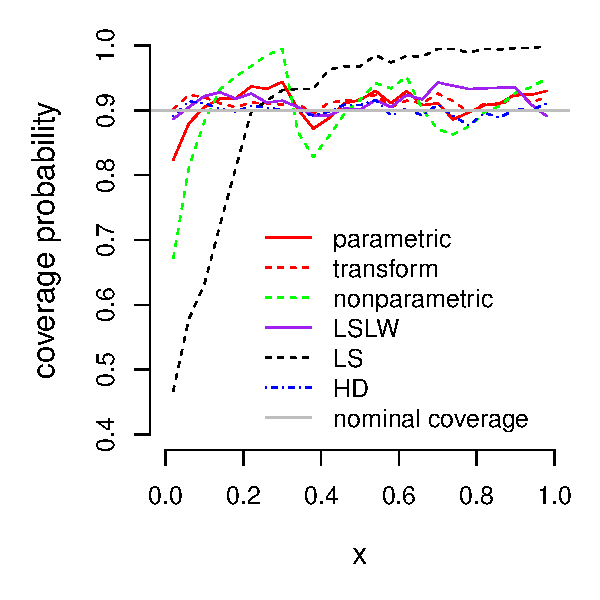
\includegraphics[width=\maxwidth]{figure/readme-inx-1} 

\end{knitrout}
\end{center}
\caption{Plot of the estimated coverage probabilities of prediction regions 
  across $x$.}
\label{Fig:coverageinx500.3}
\end{figure}




\newpage
\section{Predicting the risk of diabetes}
\label{sec:diabetes}

In this Section we reproduce the data analysis that appears in Section 6 of 
\citet{eck2019conformal}.  
We examine the influence of several variables on blood sugar, or glycosylated 
hemoglobin percentage (also known as HbA1c), an important risk factor for 
diabetes.  A glycosylated hemoglobin value of 6.5\% can be used as a cutoff 
for positive diagnosis of diabetes \citep{world2011use}. 

We predict an individual's glycosylated hemoglobin from their height, 
weight, age, and gender, all of which are easy to measure, inexpensive, and do 
not require any laboratory testing.  
The data in this analysis come from a population-based sample of 403 rural 
African-Americans in Virginia \citep{willems1997prevalence}, taken from the 
\texttt{faraway} R package \citep{faraway2016R}.  
We considered a gamma regression model that only includes linear terms for 
each covariate, a linear regression model with homoskedastic normal errors 
and the same linear terms for each covariate, and a linear regression model 
with homoskedastic normal errors that also included quadratic terms for 
each covariate.
Of these considered the models, the gamma regression model fit the data 
best on the basis that it had the lowest AIC value and it gave the best 
predictive predictive performance on the basis that it had the lowest 
sum of squares prediction error.  
That being said, we do not know the data generating process.

Based on these covariates, conformal prediction regions provide finite sample 
valid prediction regions for glycosylated hemoglobin that may be useful for 
diagnosing diabetes in this study population.
The data set is loaded from the R package \citet{faraway2016R}.

\begin{knitrout}
\definecolor{shadecolor}{rgb}{0.969, 0.969, 0.969}\color{fgcolor}\begin{kframe}
\begin{alltt}
\hlkwd{data}\hlstd{(diabetes)}
\end{alltt}
\end{kframe}
\end{knitrout}

We throw away data points that contain missing values of any variable of 
interest.

\begin{knitrout}
\definecolor{shadecolor}{rgb}{0.969, 0.969, 0.969}\color{fgcolor}\begin{kframe}
\begin{alltt}
\hlstd{dat} \hlkwb{<-} \hlstd{diabetes[,} \hlkwd{c}\hlstd{(}\hlstr{"glyhb"}\hlstd{,} \hlstr{"height"}\hlstd{,} \hlstr{"weight"}\hlstd{,} \hlstr{"age"}\hlstd{,} \hlstr{"gender"}\hlstd{)]}
\hlstd{dat} \hlkwb{<-} \hlstd{dat[}\hlkwd{complete.cases}\hlstd{(dat), ]}
\end{alltt}
\end{kframe}
\end{knitrout}


The Gamma regression model with with log link function is selected among 
several candidate models as the model used for inference in this analysis.
This model has the lowest AIC value among candidates.


\begin{knitrout}
\definecolor{shadecolor}{rgb}{0.969, 0.969, 0.969}\color{fgcolor}\begin{kframe}
\begin{alltt}
\hlstd{m.gamma.log} \hlkwb{<-} \hlkwd{glm}\hlstd{(glyhb} \hlopt{~} \hlstd{height} \hlopt{+} \hlstd{weight} \hlopt{+} \hlstd{age} \hlopt{+} \hlstd{gender,}
  \hlkwc{data} \hlstd{= dat,} \hlkwc{family} \hlstd{=} \hlkwd{Gamma}\hlstd{(}\hlkwc{link} \hlstd{= log))}
\hlstd{m.gamma} \hlkwb{<-} \hlkwd{glm}\hlstd{(glyhb} \hlopt{~} \hlstd{height} \hlopt{+} \hlstd{weight} \hlopt{+} \hlstd{age} \hlopt{+} \hlstd{gender,}
  \hlkwc{data} \hlstd{= dat,} \hlkwc{family} \hlstd{=} \hlstr{"Gamma"}\hlstd{)}
\hlstd{m.gamma.identity} \hlkwb{<-} \hlkwd{glm}\hlstd{(glyhb} \hlopt{~} \hlstd{height} \hlopt{+} \hlstd{weight} \hlopt{+} \hlstd{age} \hlopt{+} \hlstd{gender,}
  \hlkwc{data} \hlstd{= dat,} \hlkwc{family} \hlstd{=} \hlkwd{Gamma}\hlstd{(}\hlkwc{link} \hlstd{= identity))}
\hlstd{m.gaussian} \hlkwb{<-} \hlkwd{glm}\hlstd{(glyhb} \hlopt{~} \hlstd{height} \hlopt{+} \hlstd{weight} \hlopt{+} \hlstd{age} \hlopt{+} \hlstd{gender,}
  \hlkwc{data} \hlstd{= dat,} \hlkwc{family} \hlstd{=} \hlstr{"gaussian"}\hlstd{,} \hlkwc{x} \hlstd{=} \hlnum{TRUE}\hlstd{)}
\hlstd{X} \hlkwb{<-} \hlstd{m.gaussian}\hlopt{$}\hlstd{x}
\hlstd{m.gaussian.2} \hlkwb{<-} \hlkwd{glm}\hlstd{(glyhb} \hlopt{~} \hlstd{height} \hlopt{+} \hlstd{weight} \hlopt{+} \hlstd{age} \hlopt{+} \hlkwd{I}\hlstd{(height}\hlopt{^}\hlnum{2}\hlstd{)}
  \hlopt{+} \hlkwd{I}\hlstd{(weight}\hlopt{^}\hlnum{2}\hlstd{)} \hlopt{+} \hlkwd{I}\hlstd{(age}\hlopt{^}\hlnum{2}\hlstd{)} \hlopt{+} \hlstd{gender,}
  \hlkwc{data} \hlstd{= dat,} \hlkwc{family} \hlstd{=} \hlstr{"gaussian"}\hlstd{,} \hlkwc{x} \hlstd{=} \hlnum{TRUE}\hlstd{)}

\hlkwd{AIC}\hlstd{(m.gamma.log, m.gamma, m.gamma.identity, m.gaussian, m.gaussian.2)}
\end{alltt}
\begin{verbatim}
##                  df      AIC
## m.gamma.log       6 1452.012
## m.gamma           6 1452.328
## m.gamma.identity  6 1453.972
## m.gaussian        6 1644.621
## m.gaussian.2      9 1648.256
\end{verbatim}
\end{kframe}
\end{knitrout}


This model also provides satisfactory prediction as seen in 
Figure~\ref{diabetes:diagnostics}.


\begin{figure}
\begin{center}
\begin{knitrout}
\definecolor{shadecolor}{rgb}{0.969, 0.969, 0.969}\color{fgcolor}
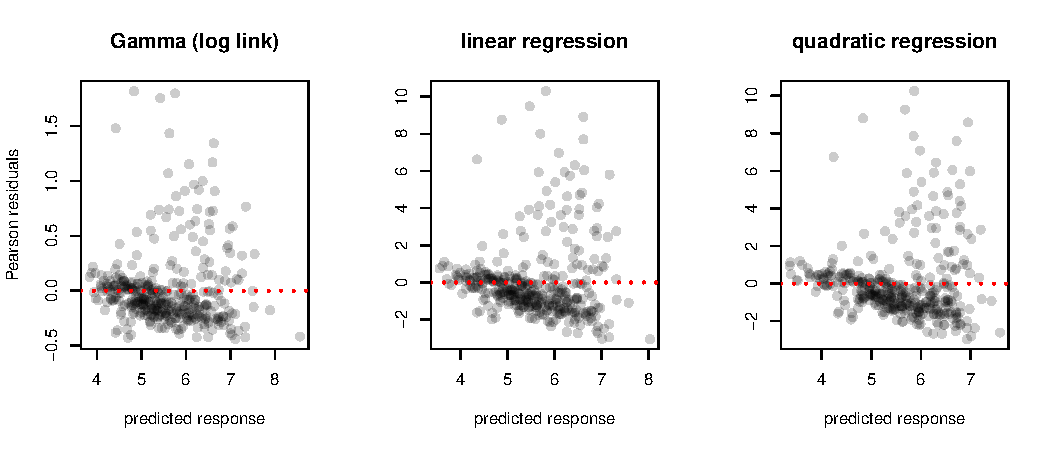
\includegraphics[width=\maxwidth]{figure/unnamed-chunk-10-1} 

\end{knitrout}
\end{center}
\caption{Predictive performance of candidate models.}
\label{diabetes:diagnostics}
\end{figure}


Six conformal prediction regions are considered for predicting glycosylated 
hemoglobin percentage.  These conformal prediction regions are the binned and 
transformation parametric conformal prediction region with a Gamma model fit, 
the binned and transformation parametric conformal prediction region with a 
Gaussian model fit, the least squares conformal prediction region, 
and the least square conformal prediction region with local weighting.  
All conformal prediction regions correspond to models that only include 
linear terms for each of the covariates.  
The binned Gamma and Gaussian parametric conformal prediction regions were 
computed with binning across the binary gender factor variable, the predictor 
space is partitioned across genders. 
However, no additional binning structure within the levels of gender was 
employed.  


These conformal prediction regions are now constructed.


\begin{knitrout}
\definecolor{shadecolor}{rgb}{0.969, 0.969, 0.969}\color{fgcolor}\begin{kframe}
\begin{alltt}
\hlcom{## Gamma conformal}
\hlkwd{system.time}\hlstd{(conformal.gamma} \hlkwb{<-}
  \hlkwd{conformal.glm}\hlstd{(m.gamma.log,} \hlkwc{cores} \hlstd{=} \hlnum{6}\hlstd{,} \hlkwc{bins} \hlstd{=} \hlnum{1}\hlstd{,}
    \hlkwc{method} \hlstd{=} \hlstr{"both"}\hlstd{))}
\end{alltt}
\begin{verbatim}
##    user  system elapsed 
## 805.660   0.913 151.499
\end{verbatim}
\begin{alltt}
\hlstd{gamma.paraconfbin} \hlkwb{<-} \hlstd{conformal.gamma}\hlopt{$}\hlstd{paraconfbin}
\hlstd{gamma.transform} \hlkwb{<-} \hlstd{conformal.gamma}\hlopt{$}\hlstd{transformconf}
\hlkwd{head}\hlstd{(gamma.paraconfbin)}
\end{alltt}
\begin{verbatim}
##        lwr      upr
## [1,] 2.485 7.352500
## [2,] 2.545 7.495000
## [3,] 3.590 9.620031
## [4,] 2.925 8.752500
## [5,] 3.270 9.400000
## [6,] 2.500 7.777500
\end{verbatim}
\begin{alltt}
\hlkwd{head}\hlstd{(gamma.transform)}
\end{alltt}
\begin{verbatim}
##           lwr       upr
## [1,] 3.112995  7.807848
## [2,] 3.186762  8.064868
## [3,] 4.253349 10.786782
## [4,] 3.707534  9.338419
## [5,] 4.051886 10.160153
## [6,] 3.226689  8.169503
\end{verbatim}
\begin{alltt}
\hlcom{## Gaussian conformal}
\hlkwd{system.time}\hlstd{(conformal.gaussian} \hlkwb{<-}
  \hlkwd{conformal.glm}\hlstd{(m.gaussian,} \hlkwc{cores} \hlstd{=} \hlnum{6}\hlstd{,} \hlkwc{bins} \hlstd{=} \hlnum{1}\hlstd{,}
    \hlkwc{method} \hlstd{=} \hlstr{"both"}\hlstd{))}
\end{alltt}
\begin{verbatim}
##    user  system elapsed 
## 413.969   0.888  73.228
\end{verbatim}
\begin{alltt}
\hlstd{gaussian.paraconfbin} \hlkwb{<-} \hlstd{conformal.gaussian}\hlopt{$}\hlstd{paraconfbin}
\hlstd{gaussian.transform} \hlkwb{<-} \hlstd{conformal.gaussian}\hlopt{$}\hlstd{transformconf}
\hlkwd{head}\hlstd{(gaussian.paraconfbin)}
\end{alltt}
\begin{verbatim}
##        lwr      upr
## [1,] 2.015 7.862500
## [2,] 2.130 8.012500
## [3,] 3.670 9.625027
## [4,] 2.925 8.880000
## [5,] 3.445 9.390000
## [6,] 2.190 8.092500
\end{verbatim}
\begin{alltt}
\hlkwd{head}\hlstd{(gaussian.transform)}
\end{alltt}
\begin{verbatim}
##           lwr       upr
## [1,] 2.569146  9.189792
## [2,] 2.748739  9.399384
## [3,] 4.349760 11.010405
## [4,] 3.535198 10.170843
## [5,] 4.033451 10.649097
## [6,] 2.801680  9.462326
\end{verbatim}
\begin{alltt}
\hlcom{## LS conformal}
\hlstd{funs} \hlkwb{<-} \hlkwd{lm.funs}\hlstd{(}\hlkwc{intercept} \hlstd{=} \hlnum{TRUE}\hlstd{)}
\hlstd{train.fun} \hlkwb{<-} \hlstd{funs}\hlopt{$}\hlstd{train.fun}
\hlstd{predict.fun} \hlkwb{<-} \hlstd{funs}\hlopt{$}\hlstd{predict.fun}
\hlstd{alpha} \hlkwb{<-} \hlnum{0.10}
\hlstd{y} \hlkwb{<-} \hlstd{dat}\hlopt{$}\hlstd{glyhb}
\hlkwd{system.time}\hlstd{(p1.tibs} \hlkwb{<-} \hlkwd{conformal.pred}\hlstd{(}\hlkwc{x} \hlstd{= X[,} \hlopt{-}\hlnum{1}\hlstd{],}
  \hlkwc{y} \hlstd{= y,} \hlkwc{x0} \hlstd{= X[,} \hlopt{-}\hlnum{1}\hlstd{],}
  \hlkwc{train.fun} \hlstd{= train.fun,} \hlkwc{predict.fun} \hlstd{= predict.fun,}
  \hlkwc{alpha} \hlstd{= alpha))}
\end{alltt}
\begin{verbatim}
##    user  system elapsed 
##   4.433   0.000   4.432
\end{verbatim}
\begin{alltt}
\hlstd{LS} \hlkwb{=} \hlkwd{cbind}\hlstd{(p1.tibs}\hlopt{$}\hlstd{lo, p1.tibs}\hlopt{$}\hlstd{up)}
\hlkwd{colnames}\hlstd{(LS)} \hlkwb{<-} \hlkwd{c}\hlstd{(}\hlstr{"lwr"}\hlstd{,} \hlstr{"upr"}\hlstd{)}
\hlkwd{head}\hlstd{(LS)}
\end{alltt}
\begin{verbatim}
##           lwr      upr
## [1,] 2.237500 7.526137
## [2,] 2.644318 7.526137
## [3,] 3.864773 9.153409
## [4,] 3.051136 8.339773
## [5,] 3.864773 9.153409
## [6,] 2.644318 7.932955
\end{verbatim}
\begin{alltt}
\hlcom{## LSLW conformal}
\hlstd{mad.train.fun} \hlkwb{<-} \hlkwa{function}\hlstd{(}\hlkwc{x}\hlstd{,} \hlkwc{y}\hlstd{,} \hlkwc{out} \hlstd{=} \hlkwa{NULL}\hlstd{)\{}
  \hlkwd{lm}\hlstd{(y} \hlopt{~} \hlstd{x[,} \hlopt{-}\hlnum{1}\hlstd{],} \hlkwc{x} \hlstd{=} \hlnum{TRUE}\hlstd{,} \hlkwc{y} \hlstd{=} \hlnum{TRUE}\hlstd{)}
\hlstd{\}}
\hlstd{mad.predict.fun} \hlkwb{<-} \hlkwa{function}\hlstd{(}\hlkwc{out}\hlstd{,} \hlkwc{newx}\hlstd{)\{}
  \hlkwd{predict}\hlstd{(out,} \hlkwd{as.data.frame}\hlstd{(newx))}
\hlstd{\}}
\hlkwd{system.time}\hlstd{(p2.tibs} \hlkwb{<-} \hlkwd{conformal.pred}\hlstd{(}\hlkwc{x} \hlstd{= X[,} \hlopt{-}\hlnum{1}\hlstd{],}
  \hlkwc{y} \hlstd{= y,} \hlkwc{x0} \hlstd{= X[,} \hlopt{-}\hlnum{1}\hlstd{],}
  \hlkwc{train.fun} \hlstd{= train.fun,} \hlkwc{predict.fun} \hlstd{= predict.fun,}
  \hlkwc{mad.train.fun} \hlstd{= mad.train.fun,}
  \hlkwc{mad.predict.fun} \hlstd{= mad.predict.fun,}
  \hlkwc{alpha} \hlstd{= alpha))}
\end{alltt}
\begin{verbatim}
##    user  system elapsed 
##  49.123   0.000  49.125
\end{verbatim}
\begin{alltt}
\hlstd{LSLW} \hlkwb{=} \hlkwd{cbind}\hlstd{(p2.tibs}\hlopt{$}\hlstd{lo, p2.tibs}\hlopt{$}\hlstd{up)}
\hlkwd{colnames}\hlstd{(LSLW)} \hlkwb{<-} \hlkwd{c}\hlstd{(}\hlstr{"lwr"}\hlstd{,} \hlstr{"upr"}\hlstd{)}
\hlkwd{head}\hlstd{(LSLW)}
\end{alltt}
\begin{verbatim}
##           lwr       upr
## [1,] 3.051136  6.712500
## [2,] 3.051136  7.119318
## [3,] 2.237500 11.187500
## [4,] 2.644318  9.153409
## [5,] 2.237500 10.373864
## [6,] 3.051136  7.119318
\end{verbatim}
\end{kframe}
\end{knitrout}


We also consider the highest density prediction region under the Gamma 
model, this region is constructed below.

\begin{knitrout}
\definecolor{shadecolor}{rgb}{0.969, 0.969, 0.969}\color{fgcolor}\begin{kframe}
\begin{alltt}
\hlcom{## HD region}
\hlkwd{library}\hlstd{(HDInterval)}
\hlstd{betaMLE} \hlkwb{<-} \hlkwd{coefficients}\hlstd{(m.gamma.log)}
\hlstd{shapeMLE} \hlkwb{<-} \hlkwd{as.numeric}\hlstd{(}\hlkwd{gamma.shape}\hlstd{(m.gamma.log)[}\hlnum{1}\hlstd{])}
\hlstd{rateMLE} \hlkwb{<-} \hlstd{(}\hlnum{1} \hlopt{/} \hlkwd{exp}\hlstd{(X} \hlopt \hlstd{betaMLE))} \hlopt{*} \hlstd{shapeMLE}
\hlcom{#rateMLE <- cbind(1, x) %*% betaMLE * shapeMLE}
\hlstd{HD} \hlkwb{<-} \hlkwd{do.call}\hlstd{(rbind,}
  \hlkwd{lapply}\hlstd{(}\hlnum{1}\hlopt{:}\hlkwd{nrow}\hlstd{(X),} \hlkwa{function}\hlstd{(}\hlkwc{j}\hlstd{)\{}
    \hlkwd{hdi}\hlstd{(qgamma,} \hlnum{0.90}\hlstd{,} \hlkwc{shape} \hlstd{= shapeMLE,} \hlkwc{rate} \hlstd{= rateMLE[j,} \hlnum{1}\hlstd{])}
  \hlstd{\}))}
\hlkwd{colnames}\hlstd{(HD)} \hlkwb{<-} \hlkwd{c}\hlstd{(}\hlstr{"lwr"}\hlstd{,} \hlstr{"upr"}\hlstd{)}
\hlkwd{head}\hlstd{(HD)}
\end{alltt}
\begin{verbatim}
##           lwr      upr
## [1,] 2.556343 7.182955
## [2,] 2.628804 7.386560
## [3,] 3.510997 9.865393
## [4,] 3.050565 8.571645
## [5,] 3.328264 9.351939
## [6,] 2.659659 7.473256
\end{verbatim}
\end{kframe}
\end{knitrout}



\subsection{Results in \citet{eck2019conformal}}

Diagnostics from the six conformal prediction regions are depicted in 
Table 2 of the manuscript \citet{eck2019conformal}.  The error tolerance 
for all prediction regions was set at $\alpha = 0.10$.  We see that 
parametric conformal prediction regions maintain their advertised finite 
sample marginal validity for the predictions of glycosylated hemoglobin.  
These prediction regions provide a balance between marginal coverage, size, 
prediction error, and average conditional coverage (the average of the 
coverage probabilities taken over small subregions of the predictor space).  
The transformation Gamma conformal prediction region balances these criteria 
particularly nicely. This prediction region is relatively small, has relatively 
small prediction error, and it gives near nominal desired coverage.  This 
finding is expected when the underlying estimated density used as the 
parametric conformity measure is a good approximation of the data generating 
model.


We now compute the diagnostics of these six conformal prediction 
regions and the highest density prediction region, and we reproduce 
Table 2 in \citet{eck2019conformal}.  
We start with the computation of marginal and approximate average 
conditional coverage using functionality in the \texttt{conformal.glm} 
software.


\begin{knitrout}
\definecolor{shadecolor}{rgb}{0.969, 0.969, 0.969}\color{fgcolor}\begin{kframe}
\begin{alltt}
\hlcom{## marginal coverages}
\hlstd{marginal.gamma.trans} \hlkwb{<-} \hlkwd{local.coverage}\hlstd{(}\hlkwc{region} \hlstd{= gamma.transform,}
  \hlkwc{data} \hlstd{= dat,} \hlkwc{bins} \hlstd{=} \hlnum{1}\hlstd{,} \hlkwc{d} \hlstd{=} \hlnum{2}\hlstd{)}
\hlstd{marginal.gaussian.trans} \hlkwb{<-} \hlkwd{local.coverage}\hlstd{(}
  \hlkwc{region} \hlstd{= gaussian.transform,} \hlkwc{data} \hlstd{= dat,} \hlkwc{bins} \hlstd{=} \hlnum{1}\hlstd{,} \hlkwc{d} \hlstd{=} \hlnum{2}\hlstd{)}
\hlstd{marginal.gamma.bin} \hlkwb{<-} \hlkwd{local.coverage}\hlstd{(}\hlkwc{region} \hlstd{= gamma.paraconfbin,}
  \hlkwc{data} \hlstd{= dat,} \hlkwc{bins} \hlstd{=} \hlnum{1}\hlstd{,} \hlkwc{d} \hlstd{=} \hlnum{2}\hlstd{)}
\hlstd{marginal.gaussian.bin} \hlkwb{<-} \hlkwd{local.coverage}\hlstd{(}\hlkwc{region} \hlstd{= gaussian.paraconfbin,}
  \hlkwc{data} \hlstd{= dat,} \hlkwc{bins} \hlstd{=} \hlnum{1}\hlstd{,} \hlkwc{d} \hlstd{=} \hlnum{2}\hlstd{)}
\hlstd{marginal.LS} \hlkwb{<-} \hlkwd{local.coverage}\hlstd{(}\hlkwc{region} \hlstd{= LS,} \hlkwc{data} \hlstd{= dat,} \hlkwc{bins} \hlstd{=} \hlnum{1}\hlstd{,} \hlkwc{d} \hlstd{=} \hlnum{2}\hlstd{)}
\hlstd{marginal.LSLW} \hlkwb{<-} \hlkwd{local.coverage}\hlstd{(}\hlkwc{region} \hlstd{= LSLW,} \hlkwc{data} \hlstd{= dat,} \hlkwc{bins} \hlstd{=} \hlnum{1}\hlstd{,} \hlkwc{d} \hlstd{=} \hlnum{2}\hlstd{)}
\hlstd{marginal.HD} \hlkwb{<-} \hlkwd{local.coverage}\hlstd{(}\hlkwc{region} \hlstd{= HD,} \hlkwc{data} \hlstd{= dat,} \hlkwc{bins} \hlstd{=} \hlnum{1}\hlstd{,} \hlkwc{d} \hlstd{=} \hlnum{2}\hlstd{)}
\hlstd{table.marginal} \hlkwb{<-} \hlkwd{matrix}\hlstd{(}\hlkwd{c}\hlstd{(marginal.gamma.trans, marginal.gaussian.trans,}
  \hlstd{marginal.gamma.bin, marginal.gaussian.bin, marginal.LSLW, marginal.LS,}
  \hlstd{marginal.HD),} \hlkwc{ncol} \hlstd{=} \hlnum{7}\hlstd{)}
\hlstd{table.marginal} \hlkwb{<-} \hlkwd{round}\hlstd{(table.marginal,} \hlnum{3}\hlstd{)}
\hlkwd{colnames}\hlstd{(table.marginal)} \hlkwb{<-} \hlkwd{c}\hlstd{(}\hlstr{"gamma trans"}\hlstd{,} \hlstr{"gaussian trans"}\hlstd{,} \hlstr{"gamma bin"}\hlstd{,}
  \hlstr{"gaussian bin"}\hlstd{,} \hlstr{"LSLW"}\hlstd{,} \hlstr{"LS"}\hlstd{,} \hlstr{"HD"}\hlstd{)}
\hlkwd{rownames}\hlstd{(table.marginal)} \hlkwb{<-} \hlstr{"marginal coverage"}

\hlcom{## conditional coverages}
\hlstd{d} \hlkwb{<-} \hlkwd{ncol}\hlstd{(dat)} \hlopt{-} \hlnum{2}
\hlstd{conditional.gamma.trans} \hlkwb{<-} \hlkwd{local.coverage}\hlstd{(}\hlkwc{region} \hlstd{= gamma.transform,}
  \hlkwc{data} \hlstd{= dat,} \hlkwc{bins} \hlstd{=} \hlnum{3}\hlstd{,} \hlkwc{d} \hlstd{= d)}
\hlstd{conditional.gaussian.trans} \hlkwb{<-} \hlkwd{local.coverage}\hlstd{(}
  \hlkwc{region} \hlstd{= gaussian.transform,} \hlkwc{data} \hlstd{= dat,} \hlkwc{bins} \hlstd{=} \hlnum{3}\hlstd{,} \hlkwc{d} \hlstd{= d)}
\hlstd{conditional.gamma.bin} \hlkwb{<-} \hlkwd{local.coverage}\hlstd{(}\hlkwc{region} \hlstd{= gamma.paraconfbin,}
  \hlkwc{data} \hlstd{= dat,} \hlkwc{bins} \hlstd{=} \hlnum{3}\hlstd{,} \hlkwc{d} \hlstd{= d)}
\hlstd{conditional.gaussian.bin} \hlkwb{<-} \hlkwd{local.coverage}\hlstd{(}\hlkwc{region} \hlstd{= gaussian.paraconfbin,}
  \hlkwc{data} \hlstd{= dat,} \hlkwc{bins} \hlstd{=} \hlnum{3}\hlstd{,} \hlkwc{d} \hlstd{= d)}
\hlstd{conditional.LS} \hlkwb{<-} \hlkwd{local.coverage}\hlstd{(}\hlkwc{region} \hlstd{= LS,} \hlkwc{data} \hlstd{= dat,} \hlkwc{bins} \hlstd{=} \hlnum{3}\hlstd{,} \hlkwc{d} \hlstd{= d)}
\hlstd{conditional.LSLW} \hlkwb{<-} \hlkwd{local.coverage}\hlstd{(}\hlkwc{region} \hlstd{= LSLW,} \hlkwc{data} \hlstd{= dat,} \hlkwc{bins} \hlstd{=} \hlnum{3}\hlstd{,} \hlkwc{d} \hlstd{= d)}
\hlstd{conditional.HD} \hlkwb{<-} \hlkwd{local.coverage}\hlstd{(}\hlkwc{region} \hlstd{= HD,} \hlkwc{data} \hlstd{= dat,} \hlkwc{bins} \hlstd{=} \hlnum{3}\hlstd{,} \hlkwc{d} \hlstd{= d)}
\hlstd{table.conditional} \hlkwb{<-} \hlkwd{matrix}\hlstd{(}\hlkwd{cbind}\hlstd{(conditional.gamma.trans,}
  \hlstd{conditional.gaussian.trans, conditional.gamma.bin, conditional.gaussian.bin,}
  \hlstd{conditional.LSLW, conditional.LS, conditional.HD),} \hlkwc{ncol} \hlstd{=} \hlnum{7}\hlstd{)}
\hlstd{table.conditional} \hlkwb{<-} \hlkwd{round}\hlstd{(table.conditional,} \hlnum{3}\hlstd{)}
\hlkwd{colnames}\hlstd{(table.conditional)} \hlkwb{<-} \hlkwd{c}\hlstd{(}\hlstr{"gamma trans"}\hlstd{,} \hlstr{"gaussian trans"}\hlstd{,}
  \hlstr{"gamma bin"}\hlstd{,} \hlstr{"gaussian bin"}\hlstd{,} \hlstr{"LSLW"}\hlstd{,} \hlstr{"LS"}\hlstd{,} \hlstr{"HD"}\hlstd{)}
\hlstd{avg.cond.coverage} \hlkwb{<-} \hlkwd{colMeans}\hlstd{(table.conditional,}\hlkwc{na.rm} \hlstd{=} \hlnum{TRUE}\hlstd{)}
\end{alltt}
\end{kframe}
\end{knitrout}


We now compute the prediction error of each conformal prediction region.

\begin{knitrout}
\definecolor{shadecolor}{rgb}{0.969, 0.969, 0.969}\color{fgcolor}\begin{kframe}
\begin{alltt}
\hlstd{pred.error.gamma.trans} \hlkwb{<-} \hlkwd{absolute.error}\hlstd{(}\hlkwc{y} \hlstd{= dat}\hlopt{$}\hlstd{glyhb,} \hlkwc{region} \hlstd{= gamma.transform)}
\hlstd{pred.error.gaussian.trans} \hlkwb{<-} \hlkwd{absolute.error}\hlstd{(}\hlkwc{y} \hlstd{= y,} \hlkwc{region} \hlstd{= gaussian.transform)}
\hlstd{pred.error.gamma.bin} \hlkwb{<-} \hlkwd{absolute.error}\hlstd{(}\hlkwc{y} \hlstd{= dat}\hlopt{$}\hlstd{glyhb,} \hlkwc{region} \hlstd{= gamma.paraconfbin)}
\hlstd{pred.error.gaussian.bin} \hlkwb{<-} \hlkwd{absolute.error}\hlstd{(}\hlkwc{y} \hlstd{= y,} \hlkwc{region} \hlstd{= gaussian.paraconfbin)}
\hlstd{pred.error.LSLW} \hlkwb{<-} \hlkwd{absolute.error}\hlstd{(}\hlkwc{y} \hlstd{= y,} \hlkwc{region} \hlstd{= LSLW)}
\hlstd{pred.error.LS} \hlkwb{<-} \hlkwd{absolute.error}\hlstd{(}\hlkwc{y} \hlstd{= y,} \hlkwc{region} \hlstd{= LS)}
\hlstd{pred.error.HD} \hlkwb{<-} \hlkwd{absolute.error}\hlstd{(}\hlkwc{y} \hlstd{= y,} \hlkwc{region} \hlstd{= HD)}
\hlstd{table.pred.error} \hlkwb{<-} \hlkwd{matrix}\hlstd{(}\hlkwd{c}\hlstd{(pred.error.gamma.trans, pred.error.gaussian.trans,}
  \hlstd{pred.error.gamma.bin, pred.error.gaussian.bin, pred.error.LSLW, pred.error.LS,}
  \hlstd{pred.error.HD),} \hlkwc{ncol} \hlstd{=} \hlnum{7}\hlstd{)}
\hlkwd{colnames}\hlstd{(table.pred.error)} \hlkwb{<-} \hlkwd{c}\hlstd{(}\hlstr{"gamma trans"}\hlstd{,} \hlstr{"gaussian trans"}\hlstd{,} \hlstr{"gamma bin"}\hlstd{,}
  \hlstr{"gaussian bin "}\hlstd{,} \hlstr{"LSLW"}\hlstd{,} \hlstr{"LS"}\hlstd{,} \hlstr{"HD"}\hlstd{)}
\hlkwd{rownames}\hlstd{(table.pred.error)} \hlkwb{<-} \hlstr{"pred error"}
\end{alltt}
\end{kframe}
\end{knitrout}


We now compute the volume of each conformal prediction region.


\begin{knitrout}
\definecolor{shadecolor}{rgb}{0.969, 0.969, 0.969}\color{fgcolor}\begin{kframe}
\begin{alltt}
\hlcom{## when no factor variables are present}
\hlstd{volume.regions} \hlkwb{<-} \hlkwa{function}\hlstd{(}\hlkwc{region}\hlstd{,} \hlkwc{preds}\hlstd{)\{}
  \hlkwa{if}\hlstd{(}\hlkwd{class}\hlstd{(region)} \hlopt{==} \hlstr{"list"}\hlstd{)\{}
    \hlkwd{stop}\hlstd{(}\hlstr{"Not appropriate for nonparametric conformal prediction regions"}\hlstd{)}
  \hlstd{\}}
  \hlstd{n} \hlkwb{<-} \hlkwd{nrow}\hlstd{(region)}
  \hlstd{mat} \hlkwb{<-} \hlkwd{as.matrix}\hlstd{(}\hlkwd{cbind}\hlstd{(preds, region[,} \hlnum{1}\hlstd{]))}
  \hlstd{mat2} \hlkwb{<-} \hlkwd{as.matrix}\hlstd{(}\hlkwd{cbind}\hlstd{(preds, region[,} \hlnum{2}\hlstd{]))}
  \hlstd{mat3} \hlkwb{<-} \hlkwd{rbind}\hlstd{(mat, mat2)}
  \hlstd{vol} \hlkwb{<-} \hlkwd{as.numeric}\hlstd{(}\hlkwd{convhulln}\hlstd{(mat3,} \hlkwc{option} \hlstd{=} \hlstr{"FA"}\hlstd{)}\hlopt{$}\hlstd{vol)}
  \hlstd{vol}
\hlstd{\}}

\hlstd{preds} \hlkwb{<-} \hlstd{dat[,} \hlnum{2}\hlopt{:}\hlnum{4}\hlstd{]}
\hlstd{volume.gamma.trans} \hlkwb{<-} \hlkwd{volume.regions}\hlstd{(}\hlkwc{region} \hlstd{= gamma.transform,} \hlkwc{preds} \hlstd{= preds)}
\hlstd{volume.gaussian.trans} \hlkwb{<-} \hlkwd{volume.regions}\hlstd{(}\hlkwc{region} \hlstd{= gaussian.transform,} \hlkwc{preds} \hlstd{= preds)}
\hlstd{volume.gamma.bin} \hlkwb{<-} \hlkwd{volume.regions}\hlstd{(}\hlkwc{region} \hlstd{= gamma.paraconfbin,} \hlkwc{preds} \hlstd{= preds)}
\hlstd{volume.gaussian.bin} \hlkwb{<-} \hlkwd{volume.regions}\hlstd{(}\hlkwc{region} \hlstd{= gaussian.paraconfbin,} \hlkwc{preds} \hlstd{= preds)}
\hlstd{volume.LSLW} \hlkwb{<-} \hlkwd{volume.regions}\hlstd{(}\hlkwc{region} \hlstd{= LSLW,} \hlkwc{preds} \hlstd{= preds)}
\hlstd{volume.LS} \hlkwb{<-} \hlkwd{volume.regions}\hlstd{(}\hlkwc{region} \hlstd{= LS,} \hlkwc{preds} \hlstd{= preds)}
\hlstd{volume.HD} \hlkwb{<-} \hlkwd{volume.regions}\hlstd{(}\hlkwc{region} \hlstd{= HD,} \hlkwc{preds} \hlstd{= preds)}
\hlstd{table.volume} \hlkwb{<-} \hlkwd{matrix}\hlstd{(}\hlkwd{c}\hlstd{(volume.gamma.trans, volume.gaussian.trans,}
  \hlstd{volume.gamma.bin, volume.gaussian.bin, volume.LSLW, volume.LS, volume.HD),} \hlkwc{ncol} \hlstd{=} \hlnum{7}\hlstd{)}
\hlkwd{colnames}\hlstd{(table.volume)} \hlkwb{<-} \hlkwd{c}\hlstd{(}\hlstr{"gamma trans"}\hlstd{,} \hlstr{"gaussian trans"}\hlstd{,} \hlstr{"gamma bin"}\hlstd{,}
  \hlstr{"gaussian bin"}\hlstd{,} \hlstr{"LSLW"}\hlstd{,} \hlstr{"LS"}\hlstd{,} \hlstr{"HD"}\hlstd{)}
\hlkwd{rownames}\hlstd{(table.volume)} \hlkwb{<-} \hlstr{"volume"}


\hlstd{volume.factors} \hlkwb{<-} \hlkwa{function}\hlstd{(}\hlkwc{region}\hlstd{,} \hlkwc{bins} \hlstd{=} \hlnum{1}\hlstd{,} \hlkwc{data}\hlstd{,} \hlkwc{object}\hlstd{)\{}
  \hlkwa{if}\hlstd{(}\hlkwd{class}\hlstd{(region)} \hlopt{==} \hlstr{"list"}\hlstd{)\{}
    \hlkwd{stop}\hlstd{(}\hlstr{"Not appropriate for nonparametric conformal prediction regions"}\hlstd{)}
  \hlstd{\}}
  \hlstd{n} \hlkwb{<-} \hlkwd{nrow}\hlstd{(region)}

  \hlstd{call} \hlkwb{<-} \hlstd{object}\hlopt{$}\hlstd{call}
  \hlstd{formula} \hlkwb{<-} \hlstd{call}\hlopt{$}\hlstd{formula}
  \hlstd{respname} \hlkwb{<-} \hlkwd{all.vars}\hlstd{(formula)[}\hlnum{1}\hlstd{]}
  \hlstd{index.factor.variables} \hlkwb{<-} \hlkwd{which}\hlstd{(}\hlkwd{attr}\hlstd{(}\hlkwd{terms}\hlstd{(object),} \hlstr{"dataClasses"}\hlstd{)} \hlopt{==} \hlstr{"factor"}\hlstd{)}
  \hlstd{index.numeric.variables} \hlkwb{<-} \hlkwd{which}\hlstd{(}\hlkwd{attr}\hlstd{(}\hlkwd{terms}\hlstd{(object),} \hlstr{"dataClasses"}\hlstd{)} \hlopt{==} \hlstr{"numeric"}\hlstd{)}
  \hlstd{data} \hlkwb{<-} \hlstd{data[, respname} \hlopt{!=} \hlkwd{colnames}\hlstd{(data)]}
  \hlstd{index.data.factor.variables} \hlkwb{<-} \hlkwd{which}\hlstd{(}\hlkwd{colnames}\hlstd{(data)} \hlopt \hlkwd{names}\hlstd{(index.factor.variables))}
  \hlstd{index.data.numeric.variables} \hlkwb{<-} \hlkwd{which}\hlstd{(}\hlkwd{colnames}\hlstd{(data)} \hlopt \hlkwd{names}\hlstd{(index.numeric.variables))}
  \hlstd{factors} \hlkwb{<-} \hlkwd{lapply}\hlstd{(index.data.factor.variables,} \hlkwa{function}\hlstd{(}\hlkwc{j}\hlstd{)} \hlkwd{as.numeric}\hlstd{(}\hlkwd{as.factor}\hlstd{(data[, j])))}
  \hlstd{data.by.factors} \hlkwb{<-} \hlkwd{split}\hlstd{(data, factors,} \hlkwc{drop} \hlstd{=} \hlnum{FALSE}\hlstd{)}
  \hlstd{region.by.factors} \hlkwb{<-} \hlkwd{split}\hlstd{(region, factors,} \hlkwc{drop} \hlstd{=} \hlnum{FALSE}\hlstd{)}
  \hlstd{matrix.region.by.factors} \hlkwb{<-} \hlkwd{lapply}\hlstd{(region.by.factors,} \hlkwa{function}\hlstd{(}\hlkwc{x}\hlstd{)\{}
    \hlkwd{matrix}\hlstd{(x,} \hlkwc{ncol} \hlstd{=} \hlnum{2}\hlstd{)}
  \hlstd{\})}
  \hlstd{numeric.by.factors} \hlkwb{<-} \hlkwd{lapply}\hlstd{(data.by.factors,} \hlkwa{function}\hlstd{(}\hlkwc{x}\hlstd{)\{}
    \hlstd{mat} \hlkwb{<-} \hlstd{x[, index.data.numeric.variables]}
    \hlkwd{colnames}\hlstd{(mat)} \hlkwb{<-} \hlkwd{colnames}\hlstd{(data)[index.data.numeric.variables]}
    \hlstd{mat}
  \hlstd{\})}
  \hlstd{bin.index.by.factors} \hlkwb{<-} \hlkwd{lapply}\hlstd{(data.by.factors,} \hlkwa{function}\hlstd{(}\hlkwc{x}\hlstd{)\{}
    \hlkwa{if}\hlstd{(}\hlkwd{nrow}\hlstd{(x)} \hlopt{==} \hlnum{0}\hlstd{)} \hlkwd{return}\hlstd{(}\hlnum{0}\hlstd{)}
    \hlstd{mat} \hlkwb{<-} \hlkwd{as.matrix}\hlstd{(x[, index.data.numeric.variables[}\hlopt{-}\hlnum{1}\hlstd{]],}
      \hlkwc{ncol} \hlstd{=} \hlkwd{length}\hlstd{(index.data.numeric.variables[}\hlopt{-}\hlnum{1}\hlstd{]))}
    \hlkwd{find.index}\hlstd{(}\hlkwc{mat} \hlstd{= mat,} \hlkwc{wn} \hlstd{=} \hlnum{1}\hlopt{/}\hlstd{bins,} \hlkwc{d} \hlstd{=} \hlkwd{ncol}\hlstd{(mat))}
  \hlstd{\})}

  \hlstd{volume.factor} \hlkwb{<-} \hlkwd{sapply}\hlstd{(}\hlnum{1}\hlopt{:}\hlkwd{length}\hlstd{(region.by.factors),} \hlkwa{function}\hlstd{(}\hlkwc{i}\hlstd{)\{}
    \hlstd{out} \hlkwb{<-} \hlkwd{sum}\hlstd{(}\hlkwd{sapply}\hlstd{(}\hlnum{1}\hlopt{:}\hlkwd{length}\hlstd{(}\hlkwd{unique}\hlstd{(bin.index.by.factors[[i]])),} \hlkwa{function}\hlstd{(}\hlkwc{j}\hlstd{)\{}
      \hlstd{X} \hlkwb{<-} \hlkwd{rbind}\hlstd{(}
        \hlkwd{cbind}\hlstd{(numeric.by.factors[[i]][}\hlkwd{which}\hlstd{(bin.index.by.factors[[i]]} \hlopt{==} \hlstd{j), ],}
          \hlstd{matrix.region.by.factors[[i]][}\hlkwd{which}\hlstd{(bin.index.by.factors[[i]]} \hlopt{==} \hlstd{j),} \hlnum{1}\hlstd{]),}
        \hlkwd{cbind}\hlstd{(numeric.by.factors[[i]][}\hlkwd{which}\hlstd{(bin.index.by.factors[[i]]} \hlopt{==} \hlstd{j), ],}
          \hlstd{matrix.region.by.factors[[i]][}\hlkwd{which}\hlstd{(bin.index.by.factors[[i]]} \hlopt{==} \hlstd{j),} \hlnum{2}\hlstd{])}
      \hlstd{)}
      \hlstd{X} \hlkwb{<-} \hlstd{X[,} \hlopt{-}\hlnum{1}\hlstd{]}
      \hlstd{vol} \hlkwb{<-} \hlkwd{as.numeric}\hlstd{(}\hlkwd{convhulln}\hlstd{(X,} \hlkwc{option} \hlstd{=} \hlstr{"FA"}\hlstd{)}\hlopt{$}\hlstd{vol)} \hlopt{*} \hlkwd{nrow}\hlstd{(X)} \hlopt{/} \hlstd{(}\hlnum{2}\hlopt{*}\hlstd{n)}
      \hlstd{vol}
    \hlstd{\}))}
    \hlkwd{return}\hlstd{(out)}
  \hlstd{\})}

  \hlkwd{sum}\hlstd{(volume.factor)}
\hlstd{\}}

\hlstd{volume.gamma.trans} \hlkwb{<-} \hlkwd{volume.factors}\hlstd{(}\hlkwc{region} \hlstd{= gamma.transform,}
  \hlkwc{data} \hlstd{= dat,} \hlkwc{object} \hlstd{= m.gamma.log)}
\hlstd{volume.gaussian.trans} \hlkwb{<-} \hlkwd{volume.factors}\hlstd{(gaussian.transform,}
  \hlkwc{data} \hlstd{= dat,} \hlkwc{object} \hlstd{= m.gaussian)}
\hlstd{volume.gamma.bin} \hlkwb{<-} \hlkwd{volume.factors}\hlstd{(}\hlkwc{region} \hlstd{= gamma.paraconfbin,}
  \hlkwc{data} \hlstd{= dat,} \hlkwc{object} \hlstd{= m.gamma.log)}
\hlstd{volume.gaussian.bin} \hlkwb{<-} \hlkwd{volume.factors}\hlstd{(gaussian.paraconfbin,}
  \hlkwc{data} \hlstd{= dat,} \hlkwc{object} \hlstd{= m.gaussian)}
\hlstd{volume.LSLW} \hlkwb{<-} \hlkwd{volume.factors}\hlstd{(LSLW,}
  \hlkwc{data} \hlstd{= dat,} \hlkwc{object} \hlstd{= m.gaussian)}
\hlstd{volume.LS} \hlkwb{<-} \hlkwd{volume.factors}\hlstd{(LS,}
  \hlkwc{data} \hlstd{= dat,} \hlkwc{object} \hlstd{= m.gaussian)}
\hlstd{volume.HD} \hlkwb{<-} \hlkwd{volume.factors}\hlstd{(HD,}
  \hlkwc{data} \hlstd{= dat,} \hlkwc{object} \hlstd{= m.gamma.log)}

\hlstd{table.volume} \hlkwb{<-} \hlkwd{matrix}\hlstd{(}\hlkwd{c}\hlstd{(volume.gamma.trans, volume.gaussian.trans,}
  \hlstd{volume.gamma.bin, volume.gaussian.bin, volume.LSLW, volume.LS,}
  \hlstd{volume.HD),} \hlkwc{ncol} \hlstd{=} \hlnum{7}\hlstd{)}
\hlkwd{colnames}\hlstd{(table.volume)} \hlkwb{<-} \hlkwd{c}\hlstd{(}\hlstr{"gamma trans"}\hlstd{,} \hlstr{"gaussian trans"}\hlstd{,} \hlstr{"gamma bin"}\hlstd{,}
  \hlstr{"gaussian bin"}\hlstd{,} \hlstr{"LSLW"}\hlstd{,} \hlstr{"LS"}\hlstd{,} \hlstr{"HD"}\hlstd{)}
\hlkwd{rownames}\hlstd{(table.volume)} \hlkwb{<-} \hlstr{"volume"}
\hlstd{table.volume} \hlkwb{<-} \hlstd{table.volume} \hlopt{/} \hlnum{1e4}
\end{alltt}
\end{kframe}
\end{knitrout}


Table 2 and Figure 4 in \citet{eck2019conformal} are shown below. 


\begin{kframe}
\begin{alltt}
\hlstd{diagnostics} \hlkwb{<-} \hlkwd{rbind}\hlstd{(table.marginal, table.volume,}
  \hlstd{table.pred.error, avg.cond.coverage)}
\hlcom{#diagnostics <- t(diagnostics)}
\hlkwd{xtable}\hlstd{(diagnostics,} \hlkwc{digits} \hlstd{=} \hlkwd{c}\hlstd{(}\hlnum{0}\hlstd{,} \hlnum{3}\hlstd{,} \hlnum{3}\hlstd{,} \hlnum{3}\hlstd{,} \hlnum{3}\hlstd{,} \hlnum{3}\hlstd{,} \hlnum{3}\hlstd{,} \hlnum{3}\hlstd{))}
\end{alltt}
\end{kframe}% latex table generated in R 3.4.4 by xtable 1.8-3 package
% Mon Oct  7 13:40:03 2019
\begin{table}[ht]
\centering
\begin{tabular}{rrrrrrrr}
  \hline
 & gamma trans & gaussian trans & gamma bin & gaussian bin & LSLW & LS & HD \\ 
  \hline
marginal coverage & 0.901 & 0.924 & 0.909 & 0.906 & 0.880 & 0.888 & 0.906 \\ 
  volume & 7.656 & 8.560 & 7.349 & 7.730 & 8.574 & 7.103 & 7.294 \\ 
  pred error & 0.653 & 0.425 & 0.931 & 0.849 & 0.803 & 1.012 & 0.948 \\ 
  avg.cond.coverage & 0.856 & 0.888 & 0.874 & 0.849 & 0.863 & 0.827 & 0.873 \\ 
   \hline
\end{tabular}
\end{table}




\begin{figure}
\begin{center}

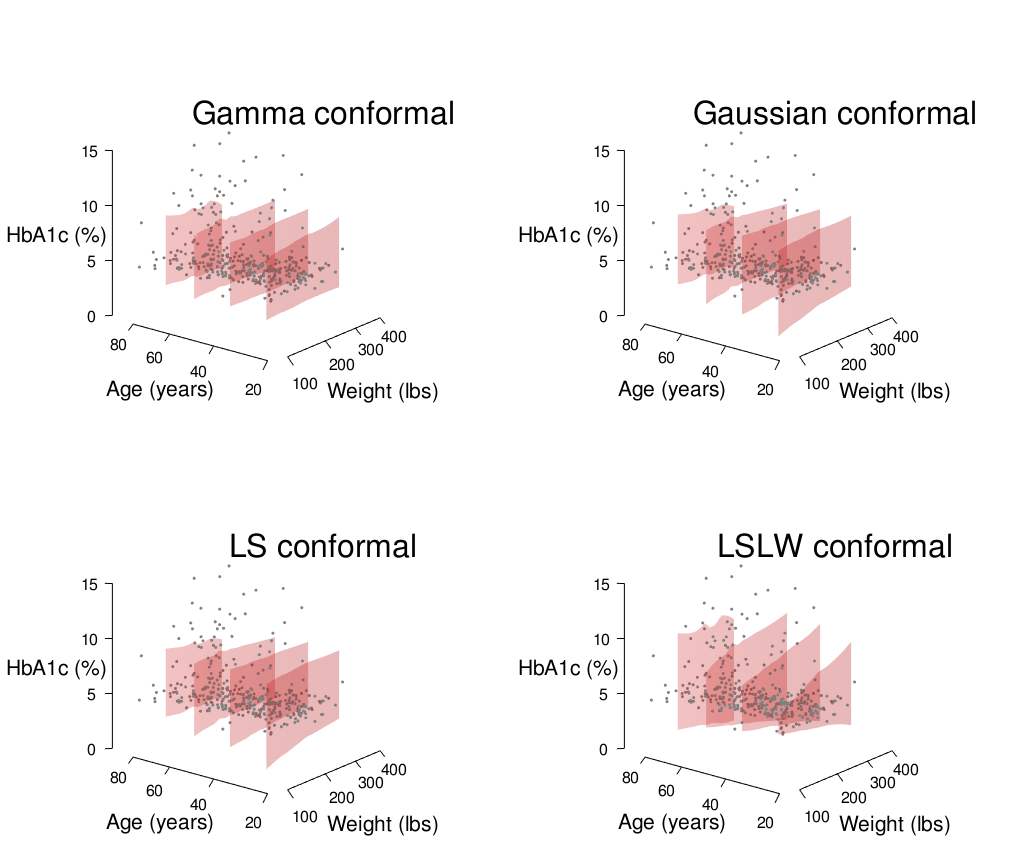
\includegraphics[width=0.9\textwidth]{conformal3ddiabetes.png}
\end{center}
\caption{ 
  Figure 4 in \citet{eck2019conformal}.
  Conformal prediction regions for glycosylated hemoglobin projected onto the 
  age and weight predictor axes.
  %People with similar ages are grouped. \comment{what do you mean that people with similar ages are grouped?  Why? } 
  Upper and lower bounds of the conformal prediction region are loess smoothed for visual appearance.
  %\comment{Why?  What do they look like if you do not smooth? }
  The code that constructed this figure is displayed in the accompanying .Rnw file.
}
\label{Fig:3d-conformal-regions}
\end{figure}





\newpage
\section{Additional Gamma simulations}
\label{sec:Gamma}

For the simulations in this section we generate responses using a gamma 
regression model with one variable.  We specify the inverse link function 
(the defualt in the \texttt{glm} function) and we set 
$\beta = (1.25, -1)^T$.  This value of $\beta$ is chosen so that the generated 
Gamma data is increasing, on average, in $x$ and exhibits increasing 
variability in $x$.  We investigate the performance of the prediction 
regions across different sample size and shape parameter combinations.  We 
consider sample sizes of $n \in \{150, 250, 500\}$ and shape parameter values 
of $\{0.5, 0.75, 1, 1.5, 2, 5, 7, 10, 12, 15, 20, 25, 30, 40, 50, 60, 70, 80, 90, 100\}$.  
The LS and LSLW conformal prediction regions are fit using a cubic regression 
model.  This model is simple and it fits this type of Gamma data better than a 
simple linear or quadratic regression model.  Note that as the shape parameter 
increases the cubic regression model fits the data better.  When $n = 150$ we 
build the parametric and nonparametric conformal prediction regions using 2 
bins.  When $n = 250, 500$ we build the parametric and nonparametric conformal 
prediction regions using 3 bins.  These number of bin choices correspond to 
the bin width asymptotics of \citet{lei2014distribution}.

The next subsection contains all the code necessary to reproduce our results 
in Section~\ref{sec:Gamma-Results}.



\subsection{Simulations}

We perform Monte Carlo simulations to investigate the coverage properties, 
size, and prediction error of the binned parametric and nonparametric 
conformal, transform under the true data generating Gamma model conformal, 
LSLW conformal, LS conformal, and HD prediction regions.  

\begin{knitrout}
\definecolor{shadecolor}{rgb}{0.969, 0.969, 0.969}\color{fgcolor}\begin{kframe}
\begin{alltt}
\hlstd{beta} \hlkwb{<-} \hlkwd{c}\hlstd{(}\hlnum{1.25}\hlstd{,} \hlopt{-}\hlnum{1}\hlstd{)}
\hlstd{gamma_simulator} \hlkwb{<-} \hlkwa{function}\hlstd{(}\hlkwc{beta}\hlstd{,} \hlkwc{n} \hlstd{=} \hlnum{150}\hlstd{,} \hlkwc{shape} \hlstd{=} \hlnum{0.5}\hlstd{,}
  \hlkwc{bins} \hlstd{=} \hlnum{2}\hlstd{,} \hlkwc{alpha} \hlstd{=} \hlnum{0.10}\hlstd{,} \hlkwc{B} \hlstd{=} \hlnum{2}\hlstd{)\{}

  \hlstd{p} \hlkwb{<-} \hlstd{d} \hlkwb{<-} \hlkwd{length}\hlstd{(beta)} \hlopt{-} \hlnum{1}

  \hlstd{models} \hlkwb{<-} \hlkwd{lapply}\hlstd{(}\hlnum{1}\hlopt{:}\hlstd{B,} \hlkwc{FUN} \hlstd{=} \hlkwa{function}\hlstd{(}\hlkwc{j}\hlstd{)\{}
    \hlstd{x} \hlkwb{<-} \hlkwd{matrix}\hlstd{(}\hlkwd{runif}\hlstd{(n}\hlopt{*}\hlstd{p),} \hlkwc{ncol} \hlstd{= p)}
    \hlstd{rate} \hlkwb{<-} \hlstd{(}\hlkwd{cbind}\hlstd{(}\hlnum{1}\hlstd{, x)} \hlopt \hlstd{beta)} \hlopt{*} \hlstd{shape}
    \hlstd{y} \hlkwb{<-} \hlkwd{rgamma}\hlstd{(}\hlkwc{n} \hlstd{= n,} \hlkwc{shape} \hlstd{= shape,} \hlkwc{rate} \hlstd{= rate)}
    \hlstd{y} \hlkwb{<-} \hlstd{y} \hlopt{/} \hlkwd{sd}\hlstd{(y)}
    \hlstd{dat} \hlkwb{<-} \hlkwd{data.frame}\hlstd{(}\hlkwc{y} \hlstd{= y,} \hlkwc{x} \hlstd{= x)}
    \hlkwd{colnames}\hlstd{(dat)[}\hlnum{2}\hlopt{:}\hlstd{(p}\hlopt{+}\hlnum{1}\hlstd{)]} \hlkwb{<-} \hlkwd{paste}\hlstd{(}\hlstr{"x"}\hlstd{,} \hlnum{1}\hlopt{:}\hlstd{p,} \hlkwc{sep} \hlstd{=} \hlstr{""}\hlstd{)}
    \hlstd{fit} \hlkwb{<-} \hlkwd{glm}\hlstd{(y} \hlopt{~} \hlstd{x1,} \hlkwc{family} \hlstd{=} \hlstr{"Gamma"}\hlstd{,} \hlkwc{data} \hlstd{= dat,}
      \hlkwc{x} \hlstd{=} \hlnum{TRUE}\hlstd{,} \hlkwc{y} \hlstd{=} \hlnum{TRUE}\hlstd{)}
    \hlstd{output} \hlkwb{=} \hlkwd{list}\hlstd{(}\hlkwc{model} \hlstd{= fit,} \hlkwc{dat} \hlstd{= dat)}
    \hlstd{output}
  \hlstd{\})}

  \hlstd{funs} \hlkwb{<-} \hlkwd{lm.funs}\hlstd{(}\hlkwc{intercept} \hlstd{=} \hlnum{TRUE}\hlstd{)}
  \hlstd{train.fun} \hlkwb{<-} \hlstd{funs}\hlopt{$}\hlstd{train.fun}
  \hlstd{predict.fun} \hlkwb{<-} \hlstd{funs}\hlopt{$}\hlstd{predict.fun}
  \hlstd{conformal_regions} \hlkwb{<-} \hlkwd{lapply}\hlstd{(models,} \hlkwc{FUN} \hlstd{=} \hlkwa{function}\hlstd{(}\hlkwc{obj}\hlstd{)\{}

    \hlstd{model} \hlkwb{<-} \hlstd{obj}\hlopt{$}\hlstd{model}
    \hlstd{dat} \hlkwb{<-} \hlstd{obj}\hlopt{$}\hlstd{dat}
    \hlstd{model}\hlopt{$}\hlstd{data} \hlkwb{<-} \hlstd{dat}
    \hlstd{x} \hlkwb{<-} \hlstd{model}\hlopt{$}\hlstd{x[,} \hlopt{-}\hlnum{1}\hlstd{]}
    \hlstd{y} \hlkwb{<-} \hlstd{model}\hlopt{$}\hlstd{y}
    \hlstd{p1.tibs} \hlkwb{<-} \hlkwd{conformal.pred}\hlstd{(}\hlkwc{x} \hlstd{=} \hlkwd{cbind}\hlstd{(x,x}\hlopt{^}\hlnum{2}\hlstd{,x}\hlopt{^}\hlnum{3}\hlstd{),} \hlkwc{y} \hlstd{= y,}
      \hlkwc{x0} \hlstd{=} \hlkwd{cbind}\hlstd{(x,x}\hlopt{^}\hlnum{2}\hlstd{,x}\hlopt{^}\hlnum{3}\hlstd{),}
      \hlkwc{train.fun} \hlstd{= train.fun,} \hlkwc{predict.fun} \hlstd{= predict.fun,}
      \hlkwc{alpha} \hlstd{= alpha)}
    \hlstd{LSCI} \hlkwb{<-} \hlkwd{cbind}\hlstd{(p1.tibs}\hlopt{$}\hlstd{lo, p1.tibs}\hlopt{$}\hlstd{up)}

    \hlstd{cubic.model} \hlkwb{<-} \hlkwd{lm}\hlstd{(y} \hlopt{~} \hlstd{x} \hlopt{+} \hlkwd{I}\hlstd{(x}\hlopt{^}\hlnum{2}\hlstd{)} \hlopt{+} \hlkwd{I}\hlstd{(x}\hlopt{^}\hlnum{3}\hlstd{))}
    \hlstd{abs.resid} \hlkwb{<-} \hlkwd{abs}\hlstd{(cubic.model}\hlopt{$}\hlstd{resid)}
    \hlstd{smooth.call} \hlkwb{<-} \hlkwd{smooth.spline}\hlstd{(x, abs.resid,}
      \hlkwc{nknots} \hlstd{=} \hlnum{10}\hlstd{)}
    \hlstd{lambda} \hlkwb{<-} \hlstd{smooth.call}\hlopt{$}\hlstd{lambda}
    \hlstd{df} \hlkwb{<-} \hlstd{smooth.call}\hlopt{$}\hlstd{df}
    \hlstd{mad.train.fun} \hlkwb{<-} \hlkwa{function}\hlstd{(}\hlkwc{x}\hlstd{,} \hlkwc{y}\hlstd{,} \hlkwc{out} \hlstd{=} \hlkwa{NULL}\hlstd{)\{}
      \hlkwd{smooth.spline}\hlstd{(x[,} \hlnum{1}\hlstd{], y,} \hlkwc{lambda} \hlstd{= lambda,}
      \hlkwc{df} \hlstd{= df,} \hlkwc{nknots} \hlstd{=} \hlnum{10}\hlstd{)}
    \hlstd{\}}
    \hlstd{mad.predict.fun} \hlkwb{<-} \hlkwa{function}\hlstd{(}\hlkwc{out}\hlstd{,} \hlkwc{newx}\hlstd{)\{}
      \hlkwd{predict}\hlstd{(out,} \hlkwd{as.data.frame}\hlstd{(newx))}\hlopt{$}\hlstd{y[,} \hlnum{1}\hlstd{]}
    \hlstd{\}}
    \hlstd{p2.tibs} \hlkwb{<-} \hlkwd{conformal.pred}\hlstd{(}\hlkwc{x} \hlstd{=} \hlkwd{cbind}\hlstd{(x,x}\hlopt{^}\hlnum{2}\hlstd{,x}\hlopt{^}\hlnum{3}\hlstd{),} \hlkwc{y} \hlstd{= y,}
      \hlkwc{x0} \hlstd{=} \hlkwd{cbind}\hlstd{(x,x}\hlopt{^}\hlnum{2}\hlstd{,x}\hlopt{^}\hlnum{3}\hlstd{),}
      \hlkwc{train.fun} \hlstd{= train.fun,} \hlkwc{predict.fun} \hlstd{= predict.fun,}
      \hlkwc{mad.train.fun} \hlstd{= mad.train.fun,}
      \hlkwc{mad.predict.fun} \hlstd{= mad.predict.fun,}
      \hlkwc{alpha} \hlstd{= alpha)}
    \hlstd{LSLWCI} \hlkwb{<-} \hlkwd{cbind}\hlstd{(p2.tibs}\hlopt{$}\hlstd{lo, p2.tibs}\hlopt{$}\hlstd{up)}

    \hlstd{betaMLE} \hlkwb{<-} \hlkwd{coefficients}\hlstd{(model)}
    \hlstd{shapeMLE} \hlkwb{<-} \hlkwd{as.numeric}\hlstd{(}\hlkwd{gamma.shape}\hlstd{(model)[}\hlnum{1}\hlstd{])}
    \hlstd{rateMLE} \hlkwb{<-} \hlkwd{cbind}\hlstd{(}\hlnum{1}\hlstd{, x)} \hlopt \hlstd{betaMLE} \hlopt{*} \hlstd{shapeMLE}
    \hlstd{HDCI} \hlkwb{<-} \hlkwd{do.call}\hlstd{(rbind,} \hlkwd{lapply}\hlstd{(}\hlnum{1}\hlopt{:}\hlstd{n,} \hlkwa{function}\hlstd{(}\hlkwc{j}\hlstd{)\{}
      \hlkwd{hdi}\hlstd{(qgamma,} \hlnum{1} \hlopt{-} \hlstd{alpha,} \hlkwc{shape} \hlstd{= shapeMLE,} \hlkwc{rate} \hlstd{= rateMLE[j,} \hlnum{1}\hlstd{])}
    \hlstd{\}))}

    \hlstd{conf} \hlkwb{<-} \hlkwd{conformal.glm}\hlstd{(model,} \hlkwc{nonparametric} \hlstd{=} \hlnum{TRUE}\hlstd{,} \hlkwc{method} \hlstd{=} \hlstr{"both"}\hlstd{,}
      \hlkwc{bins} \hlstd{= bins,} \hlkwc{cores} \hlstd{=} \hlnum{7}\hlstd{)}
    \hlstd{parabinCI} \hlkwb{<-} \hlstd{conf}\hlopt{$}\hlstd{paraconfbin}
    \hlstd{transformCI} \hlkwb{<-} \hlstd{conf}\hlopt{$}\hlstd{transformconf}
    \hlstd{nonparabinCI} \hlkwb{<-} \hlstd{conf}\hlopt{$}\hlstd{nonparaconfbin}

    \hlstd{out} \hlkwb{=} \hlkwd{list}\hlstd{(}\hlkwc{parabinCI} \hlstd{= parabinCI,} \hlkwc{transformCI} \hlstd{= transformCI,}
      \hlkwc{nonparabinCI} \hlstd{= nonparabinCI,} \hlkwc{LSLWCI} \hlstd{= LSLWCI,} \hlkwc{LSCI} \hlstd{= LSCI,}
      \hlkwc{HDCI} \hlstd{= HDCI)}
    \hlstd{out}
  \hlstd{\})}

  \hlstd{diagnostics_regions} \hlkwb{<-} \hlkwd{lapply}\hlstd{(}\hlnum{1}\hlopt{:}\hlstd{B,} \hlkwc{FUN} \hlstd{=} \hlkwa{function}\hlstd{(}\hlkwc{j}\hlstd{)\{}

    \hlstd{obj} \hlkwb{<-} \hlstd{conformal_regions[[j]]}
    \hlstd{dat} \hlkwb{<-} \hlkwd{as.data.frame}\hlstd{(models[[j]]}\hlopt{$}\hlstd{dat)}
    \hlstd{y} \hlkwb{<-} \hlkwd{as.numeric}\hlstd{(dat[,} \hlnum{1}\hlstd{])}

    \hlstd{diagnostics} \hlkwb{<-} \hlkwd{lapply}\hlstd{(obj,} \hlkwc{FUN} \hlstd{=} \hlkwa{function}\hlstd{(}\hlkwc{region}\hlstd{)\{}

      \hlstd{output} \hlkwb{<-} \hlkwa{NULL}
      \hlkwa{if}\hlstd{(}\hlkwd{class}\hlstd{(region)} \hlopt{==} \hlstr{"matrix"}\hlstd{)\{}
        \hlstd{marginal.coverage} \hlkwb{<-} \hlkwd{local.coverage}\hlstd{(}\hlkwc{region} \hlstd{= region,}
          \hlkwc{data} \hlstd{= dat,} \hlkwc{d} \hlstd{= p,} \hlkwc{bins} \hlstd{=} \hlnum{1}\hlstd{,} \hlkwc{at.data} \hlstd{=} \hlstr{"TRUE"}\hlstd{)}
        \hlstd{local.coverage} \hlkwb{<-} \hlkwd{local.coverage}\hlstd{(}\hlkwc{region} \hlstd{= region,}
          \hlkwc{data} \hlstd{= dat,} \hlkwc{d} \hlstd{= p,} \hlkwc{bins} \hlstd{= bins,} \hlkwc{at.data} \hlstd{=} \hlstr{"TRUE"}\hlstd{)}
        \hlstd{local.inx.coverage} \hlkwb{<-} \hlkwd{local.coverage}\hlstd{(}\hlkwc{region} \hlstd{= region,}
          \hlkwc{data} \hlstd{= dat,} \hlkwc{d} \hlstd{= p,} \hlkwc{bins} \hlstd{=} \hlnum{25}\hlstd{,} \hlkwc{at.data} \hlstd{=} \hlstr{"TRUE"}\hlstd{)}
        \hlstd{output} \hlkwb{<-} \hlkwd{c}\hlstd{(marginal.coverage, local.coverage,}
          \hlstd{local.inx.coverage,} \hlkwd{mean}\hlstd{(}\hlkwd{apply}\hlstd{(region,} \hlnum{1}\hlstd{, diff)),}
          \hlkwd{absolute.error}\hlstd{(}\hlkwc{y} \hlstd{= y,} \hlkwc{region} \hlstd{= region))}
      \hlstd{\}}
      \hlkwa{else}\hlstd{\{}
        \hlstd{marginal.coverage} \hlkwb{<-} \hlkwd{local.coverage}\hlstd{(}\hlkwc{region} \hlstd{= region,}
          \hlkwc{nonparametric} \hlstd{=} \hlstr{"TRUE"}\hlstd{,} \hlkwc{data} \hlstd{= dat,} \hlkwc{d} \hlstd{= p,} \hlkwc{bins} \hlstd{=} \hlnum{1}\hlstd{,}
          \hlkwc{at.data} \hlstd{=} \hlstr{"TRUE"}\hlstd{)}
        \hlstd{local.coverage} \hlkwb{<-} \hlkwd{local.coverage}\hlstd{(}\hlkwc{region} \hlstd{= region,}
          \hlkwc{nonparametric} \hlstd{=} \hlstr{"TRUE"}\hlstd{,} \hlkwc{data} \hlstd{= dat,} \hlkwc{d} \hlstd{= p,} \hlkwc{bins} \hlstd{= bins,}
          \hlkwc{at.data} \hlstd{=} \hlstr{"TRUE"}\hlstd{)}
        \hlstd{local.inx.coverage} \hlkwb{<-} \hlkwd{local.coverage}\hlstd{(}\hlkwc{region} \hlstd{= region,}
          \hlkwc{nonparametric} \hlstd{=} \hlstr{"TRUE"}\hlstd{,} \hlkwc{data} \hlstd{= dat,} \hlkwc{d} \hlstd{= p,} \hlkwc{bins} \hlstd{=} \hlnum{25}\hlstd{,}
          \hlkwc{at.data} \hlstd{=} \hlstr{"TRUE"}\hlstd{)}
        \hlstd{output} \hlkwb{<-} \hlkwd{c}\hlstd{(marginal.coverage, local.coverage,}
          \hlstd{local.inx.coverage,} \hlkwd{area.nonparametric}\hlstd{(region),}
          \hlkwd{absolute.error.nonparametric}\hlstd{(}\hlkwc{data} \hlstd{= dat,}
            \hlkwc{region} \hlstd{= region))}
      \hlstd{\}}
      \hlstd{output}
    \hlstd{\})}
    \hlkwd{do.call}\hlstd{(rbind, diagnostics)}

  \hlstd{\})}

  \hlstd{diagnostics_regions}
\hlstd{\}}
\end{alltt}
\end{kframe}
\end{knitrout}



The following performs our Monte Carlo simulation of $B = 200$ iterations 
when $n = 150$ and shape = $0.5$.

\begin{knitrout}
\definecolor{shadecolor}{rgb}{0.969, 0.969, 0.969}\color{fgcolor}\begin{kframe}
\begin{alltt}
\hlkwd{set.seed}\hlstd{(}\hlnum{13}\hlstd{)}
\hlstd{beta} \hlkwb{<-} \hlkwd{c}\hlstd{(}\hlnum{1.25}\hlstd{,} \hlopt{-}\hlnum{1}\hlstd{)}
\hlstd{bins} \hlkwb{<-} \hlnum{2}
\hlstd{B} \hlkwb{<-} \hlnum{200}
\hlstd{n} \hlkwb{<-} \hlnum{150}
\hlkwd{system.time}\hlstd{(out.gamma.150.2.0.5} \hlkwb{<-} \hlkwd{do.call}\hlstd{(rbind,}
  \hlkwd{gamma_simulator}\hlstd{(}\hlkwc{beta} \hlstd{= beta,} \hlkwc{n} \hlstd{= n,} \hlkwc{shape} \hlstd{=} \hlnum{0.5}\hlstd{,} \hlkwc{bins} \hlstd{= bins,} \hlkwc{B} \hlstd{= B)))}
\end{alltt}
\begin{verbatim}
##      user    system   elapsed 
## 16345.387   204.330  7011.362
\end{verbatim}
\begin{alltt}
\hlstd{diagnostics.150.2.0.5} \hlkwb{<-} \hlkwd{do.call}\hlstd{(rbind,} \hlkwd{lapply}\hlstd{(}\hlkwd{split}\hlstd{(out.gamma.150.2.0.5,}
  \hlkwc{f} \hlstd{=} \hlkwd{as.factor}\hlstd{(}\hlkwd{rownames}\hlstd{(out.gamma.150.2.0.5))),}
  \hlkwc{FUN} \hlstd{=} \hlkwa{function}\hlstd{(}\hlkwc{xx}\hlstd{)} \hlkwd{colMeans}\hlstd{(}\hlkwd{matrix}\hlstd{(xx,} \hlkwc{nrow} \hlstd{= B))))}
\end{alltt}
\end{kframe}
\end{knitrout}




The following performs our Monte Carlo simulation of $B = 200$ iterations 
when $n = 150$ and shape = $0.75$.

\begin{knitrout}
\definecolor{shadecolor}{rgb}{0.969, 0.969, 0.969}\color{fgcolor}\begin{kframe}
\begin{alltt}
\hlkwd{set.seed}\hlstd{(}\hlnum{13}\hlstd{)}
\hlkwd{system.time}\hlstd{(out.gamma.150.2.0.75} \hlkwb{<-} \hlkwd{do.call}\hlstd{(rbind,}
  \hlkwd{gamma_simulator}\hlstd{(}\hlkwc{beta} \hlstd{= beta,} \hlkwc{n} \hlstd{= n,} \hlkwc{shape} \hlstd{=} \hlnum{0.75}\hlstd{,} \hlkwc{bins} \hlstd{= bins,} \hlkwc{B} \hlstd{= B)))}
\end{alltt}


{\ttfamily\noindent\color{warningcolor}{\#\# Warning in log(ifelse(y == 0, 1, y/mu)): NaNs produced}}

{\ttfamily\noindent\bfseries\color{errorcolor}{\#\# Error: no valid set of coefficients has been found: please supply starting values}}

{\ttfamily\noindent\itshape\color{messagecolor}{\#\# Timing stopped at: 0.239 0 0.24}}\begin{alltt}
\hlstd{diagnostics.150.2.0.75} \hlkwb{<-} \hlkwd{do.call}\hlstd{(rbind,} \hlkwd{lapply}\hlstd{(}\hlkwd{split}\hlstd{(out.gamma.150.2.0.75,}
  \hlkwc{f} \hlstd{=} \hlkwd{as.factor}\hlstd{(}\hlkwd{rownames}\hlstd{(out.gamma.150.2.0.75))),}
  \hlkwc{FUN} \hlstd{=} \hlkwa{function}\hlstd{(}\hlkwc{xx}\hlstd{)} \hlkwd{colMeans}\hlstd{(}\hlkwd{matrix}\hlstd{(xx,} \hlkwc{nrow} \hlstd{= B))))}
\end{alltt}


{\ttfamily\noindent\bfseries\color{errorcolor}{\#\# Error in split(out.gamma.150.2.0.75, f = as.factor(rownames(out.gamma.150.2.0.75))): object 'out.gamma.150.2.0.75' not found}}\end{kframe}
\end{knitrout}




The following performs our Monte Carlo simulation of $B = 200$ iterations 
when $n = 150$ and shape = $1$.

\begin{knitrout}
\definecolor{shadecolor}{rgb}{0.969, 0.969, 0.969}\color{fgcolor}\begin{kframe}
\begin{alltt}
\hlkwd{set.seed}\hlstd{(}\hlnum{13}\hlstd{)}
\hlkwd{system.time}\hlstd{(out.gamma.150.2.1} \hlkwb{<-} \hlkwd{do.call}\hlstd{(rbind,}
  \hlkwd{gamma_simulator}\hlstd{(}\hlkwc{beta} \hlstd{= beta,} \hlkwc{n} \hlstd{= n,} \hlkwc{shape} \hlstd{=} \hlnum{1}\hlstd{,} \hlkwc{bins} \hlstd{= bins,} \hlkwc{B} \hlstd{= B)))}
\end{alltt}
\begin{verbatim}
##      user    system   elapsed 
## 16618.992   207.724  7035.463
\end{verbatim}
\begin{alltt}
\hlstd{diagnostics.150.2.1} \hlkwb{<-} \hlkwd{do.call}\hlstd{(rbind,} \hlkwd{lapply}\hlstd{(}\hlkwd{split}\hlstd{(out.gamma.150.2.1,}
  \hlkwc{f} \hlstd{=} \hlkwd{as.factor}\hlstd{(}\hlkwd{rownames}\hlstd{(out.gamma.150.2.1))),}
  \hlkwc{FUN} \hlstd{=} \hlkwa{function}\hlstd{(}\hlkwc{xx}\hlstd{)} \hlkwd{colMeans}\hlstd{(}\hlkwd{matrix}\hlstd{(xx,} \hlkwc{nrow} \hlstd{= B))))}
\end{alltt}
\end{kframe}
\end{knitrout}




The following performs our Monte Carlo simulation of $B = 200$ iterations 
when $n = 150$ and shape = $1.5$.

\begin{knitrout}
\definecolor{shadecolor}{rgb}{0.969, 0.969, 0.969}\color{fgcolor}\begin{kframe}
\begin{alltt}
\hlkwd{set.seed}\hlstd{(}\hlnum{13}\hlstd{)}
\hlkwd{system.time}\hlstd{(out.gamma.150.2.1.5} \hlkwb{<-} \hlkwd{do.call}\hlstd{(rbind,}
  \hlkwd{gamma_simulator}\hlstd{(}\hlkwc{beta} \hlstd{= beta,} \hlkwc{n} \hlstd{= n,} \hlkwc{shape} \hlstd{=} \hlnum{1.5}\hlstd{,} \hlkwc{bins} \hlstd{= bins,} \hlkwc{B} \hlstd{= B)))}
\end{alltt}
\begin{verbatim}
##      user    system   elapsed 
## 17682.956   214.156  7197.812
\end{verbatim}
\begin{alltt}
\hlstd{diagnostics.150.2.1.5} \hlkwb{<-} \hlkwd{do.call}\hlstd{(rbind,} \hlkwd{lapply}\hlstd{(}\hlkwd{split}\hlstd{(out.gamma.150.2.1.5,}
  \hlkwc{f} \hlstd{=} \hlkwd{as.factor}\hlstd{(}\hlkwd{rownames}\hlstd{(out.gamma.150.2.1.5))),}
  \hlkwc{FUN} \hlstd{=} \hlkwa{function}\hlstd{(}\hlkwc{xx}\hlstd{)} \hlkwd{colMeans}\hlstd{(}\hlkwd{matrix}\hlstd{(xx,} \hlkwc{nrow} \hlstd{= B))))}
\end{alltt}
\end{kframe}
\end{knitrout}




The following performs our Monte Carlo simulation of $B = 200$ iterations 
when $n = 150$ and shape = $2$.

\begin{knitrout}
\definecolor{shadecolor}{rgb}{0.969, 0.969, 0.969}\color{fgcolor}\begin{kframe}
\begin{alltt}
\hlkwd{set.seed}\hlstd{(}\hlnum{13}\hlstd{)}
\hlkwd{system.time}\hlstd{(out.gamma.150.2.2} \hlkwb{<-} \hlkwd{do.call}\hlstd{(rbind,}
  \hlkwd{gamma_simulator}\hlstd{(}\hlkwc{beta} \hlstd{= beta,} \hlkwc{n} \hlstd{= n,} \hlkwc{shape} \hlstd{=} \hlnum{2}\hlstd{,} \hlkwc{bins} \hlstd{= bins,} \hlkwc{B} \hlstd{= B)))}
\end{alltt}
\begin{verbatim}
##      user    system   elapsed 
## 19198.965   220.455  7458.240
\end{verbatim}
\begin{alltt}
\hlstd{diagnostics.150.2.2} \hlkwb{<-} \hlkwd{do.call}\hlstd{(rbind,} \hlkwd{lapply}\hlstd{(}\hlkwd{split}\hlstd{(out.gamma.150.2.2,}
  \hlkwc{f} \hlstd{=} \hlkwd{as.factor}\hlstd{(}\hlkwd{rownames}\hlstd{(out.gamma.150.2.2))),}
  \hlkwc{FUN} \hlstd{=} \hlkwa{function}\hlstd{(}\hlkwc{xx}\hlstd{)} \hlkwd{colMeans}\hlstd{(}\hlkwd{matrix}\hlstd{(xx,} \hlkwc{nrow} \hlstd{= B))))}
\end{alltt}
\end{kframe}
\end{knitrout}




The following performs our Monte Carlo simulation of $B = 200$ iterations 
when $n = 150$ and shape = $5$.

\begin{knitrout}
\definecolor{shadecolor}{rgb}{0.969, 0.969, 0.969}\color{fgcolor}\begin{kframe}
\begin{alltt}
\hlkwd{set.seed}\hlstd{(}\hlnum{13}\hlstd{)}
\hlkwd{system.time}\hlstd{(out.gamma.150.2.5} \hlkwb{<-} \hlkwd{do.call}\hlstd{(rbind,}
  \hlkwd{gamma_simulator}\hlstd{(}\hlkwc{beta} \hlstd{= beta,} \hlkwc{n} \hlstd{= n,} \hlkwc{shape} \hlstd{=} \hlnum{5}\hlstd{,} \hlkwc{bins} \hlstd{= bins,} \hlkwc{B} \hlstd{= B)))}
\end{alltt}
\begin{verbatim}
##      user    system   elapsed 
## 20250.447   223.468  7670.782
\end{verbatim}
\begin{alltt}
\hlstd{diagnostics.150.2.5} \hlkwb{<-} \hlkwd{do.call}\hlstd{(rbind,} \hlkwd{lapply}\hlstd{(}\hlkwd{split}\hlstd{(out.gamma.150.2.5,}
  \hlkwc{f} \hlstd{=} \hlkwd{as.factor}\hlstd{(}\hlkwd{rownames}\hlstd{(out.gamma.150.2.5))),}
  \hlkwc{FUN} \hlstd{=} \hlkwa{function}\hlstd{(}\hlkwc{xx}\hlstd{)} \hlkwd{colMeans}\hlstd{(}\hlkwd{matrix}\hlstd{(xx,} \hlkwc{nrow} \hlstd{= B))))}
\end{alltt}
\end{kframe}
\end{knitrout}




The following performs our Monte Carlo simulation of $B = 200$ iterations 
when $n = 150$ and shape = $7$.

\begin{knitrout}
\definecolor{shadecolor}{rgb}{0.969, 0.969, 0.969}\color{fgcolor}\begin{kframe}
\begin{alltt}
\hlkwd{set.seed}\hlstd{(}\hlnum{13}\hlstd{)}
\hlkwd{system.time}\hlstd{(out.gamma.150.2.7} \hlkwb{<-} \hlkwd{do.call}\hlstd{(rbind,}
  \hlkwd{gamma_simulator}\hlstd{(}\hlkwc{beta} \hlstd{= beta,} \hlkwc{n} \hlstd{= n,} \hlkwc{shape} \hlstd{=} \hlnum{7}\hlstd{,} \hlkwc{bins} \hlstd{= bins,} \hlkwc{B} \hlstd{= B)))}
\end{alltt}
\begin{verbatim}
##      user    system   elapsed 
## 19494.677   224.071  7521.206
\end{verbatim}
\begin{alltt}
\hlstd{diagnostics.150.2.7} \hlkwb{<-} \hlkwd{do.call}\hlstd{(rbind,} \hlkwd{lapply}\hlstd{(}\hlkwd{split}\hlstd{(out.gamma.150.2.7,}
  \hlkwc{f} \hlstd{=} \hlkwd{as.factor}\hlstd{(}\hlkwd{rownames}\hlstd{(out.gamma.150.2.7))),}
  \hlkwc{FUN} \hlstd{=} \hlkwa{function}\hlstd{(}\hlkwc{xx}\hlstd{)} \hlkwd{colMeans}\hlstd{(}\hlkwd{matrix}\hlstd{(xx,} \hlkwc{nrow} \hlstd{= B))))}
\end{alltt}
\end{kframe}
\end{knitrout}




The following performs our Monte Carlo simulation of $B = 200$ iterations 
when $n = 150$ and shape = $10$.

\begin{knitrout}
\definecolor{shadecolor}{rgb}{0.969, 0.969, 0.969}\color{fgcolor}\begin{kframe}
\begin{alltt}
\hlkwd{set.seed}\hlstd{(}\hlnum{13}\hlstd{)}
\hlkwd{system.time}\hlstd{(out.gamma.150.2.10} \hlkwb{<-} \hlkwd{do.call}\hlstd{(rbind,}
  \hlkwd{gamma_simulator}\hlstd{(}\hlkwc{beta} \hlstd{= beta,} \hlkwc{n} \hlstd{= n,} \hlkwc{shape} \hlstd{=} \hlnum{10}\hlstd{,} \hlkwc{bins} \hlstd{= bins,} \hlkwc{B} \hlstd{= B)))}
\end{alltt}
\begin{verbatim}
##      user    system   elapsed 
## 18152.953   217.606  7289.143
\end{verbatim}
\begin{alltt}
\hlstd{diagnostics.150.2.10} \hlkwb{<-} \hlkwd{do.call}\hlstd{(rbind,} \hlkwd{lapply}\hlstd{(}\hlkwd{split}\hlstd{(out.gamma.150.2.10,}
  \hlkwc{f} \hlstd{=} \hlkwd{as.factor}\hlstd{(}\hlkwd{rownames}\hlstd{(out.gamma.150.2.10))),}
  \hlkwc{FUN} \hlstd{=} \hlkwa{function}\hlstd{(}\hlkwc{xx}\hlstd{)} \hlkwd{colMeans}\hlstd{(}\hlkwd{matrix}\hlstd{(xx,} \hlkwc{nrow} \hlstd{= B))))}
\end{alltt}
\end{kframe}
\end{knitrout}




The following performs our Monte Carlo simulation of $B = 200$ iterations 
when $n = 150$ and shape = $12$.

\begin{knitrout}
\definecolor{shadecolor}{rgb}{0.969, 0.969, 0.969}\color{fgcolor}\begin{kframe}
\begin{alltt}
\hlkwd{set.seed}\hlstd{(}\hlnum{13}\hlstd{)}
\hlkwd{system.time}\hlstd{(out.gamma.150.2.12} \hlkwb{<-} \hlkwd{do.call}\hlstd{(rbind,}
  \hlkwd{gamma_simulator}\hlstd{(}\hlkwc{beta} \hlstd{= beta,} \hlkwc{n} \hlstd{= n,} \hlkwc{shape} \hlstd{=} \hlnum{12}\hlstd{,} \hlkwc{bins} \hlstd{= bins,} \hlkwc{B} \hlstd{= B)))}
\end{alltt}
\begin{verbatim}
##      user    system   elapsed 
## 17510.891   215.420  7175.219
\end{verbatim}
\begin{alltt}
\hlstd{diagnostics.150.2.12} \hlkwb{<-} \hlkwd{do.call}\hlstd{(rbind,} \hlkwd{lapply}\hlstd{(}\hlkwd{split}\hlstd{(out.gamma.150.2.12,}
  \hlkwc{f} \hlstd{=} \hlkwd{as.factor}\hlstd{(}\hlkwd{rownames}\hlstd{(out.gamma.150.2.12))),}
  \hlkwc{FUN} \hlstd{=} \hlkwa{function}\hlstd{(}\hlkwc{xx}\hlstd{)} \hlkwd{colMeans}\hlstd{(}\hlkwd{matrix}\hlstd{(xx,} \hlkwc{nrow} \hlstd{= B))))}
\end{alltt}
\end{kframe}
\end{knitrout}




The following performs our Monte Carlo simulation of $B = 200$ iterations 
when $n = 150$ and shape = $15$.

\begin{knitrout}
\definecolor{shadecolor}{rgb}{0.969, 0.969, 0.969}\color{fgcolor}\begin{kframe}
\begin{alltt}
\hlkwd{set.seed}\hlstd{(}\hlnum{13}\hlstd{)}
\hlkwd{system.time}\hlstd{(out.gamma.150.2.15} \hlkwb{<-} \hlkwd{do.call}\hlstd{(rbind,}
  \hlkwd{gamma_simulator}\hlstd{(}\hlkwc{beta} \hlstd{= beta,} \hlkwc{n} \hlstd{= n,} \hlkwc{shape} \hlstd{=} \hlnum{15}\hlstd{,} \hlkwc{bins} \hlstd{= bins,} \hlkwc{B} \hlstd{= B)))}
\end{alltt}
\begin{verbatim}
##      user    system   elapsed 
## 16722.807   211.209  7049.776
\end{verbatim}
\begin{alltt}
\hlstd{diagnostics.150.2.15} \hlkwb{<-} \hlkwd{do.call}\hlstd{(rbind,} \hlkwd{lapply}\hlstd{(}\hlkwd{split}\hlstd{(out.gamma.150.2.15,}
  \hlkwc{f} \hlstd{=} \hlkwd{as.factor}\hlstd{(}\hlkwd{rownames}\hlstd{(out.gamma.150.2.15))),}
  \hlkwc{FUN} \hlstd{=} \hlkwa{function}\hlstd{(}\hlkwc{xx}\hlstd{)} \hlkwd{colMeans}\hlstd{(}\hlkwd{matrix}\hlstd{(xx,} \hlkwc{nrow} \hlstd{= B))))}
\end{alltt}
\end{kframe}
\end{knitrout}




The following performs our Monte Carlo simulation of $B = 200$ iterations 
when $n = 150$ and shape = $20$.

\begin{knitrout}
\definecolor{shadecolor}{rgb}{0.969, 0.969, 0.969}\color{fgcolor}\begin{kframe}
\begin{alltt}
\hlkwd{set.seed}\hlstd{(}\hlnum{13}\hlstd{)}
\hlkwd{system.time}\hlstd{(out.gamma.150.2.20} \hlkwb{<-} \hlkwd{do.call}\hlstd{(rbind,}
  \hlkwd{gamma_simulator}\hlstd{(}\hlkwc{beta} \hlstd{= beta,} \hlkwc{n} \hlstd{= n,} \hlkwc{shape} \hlstd{=} \hlnum{20}\hlstd{,} \hlkwc{bins} \hlstd{= bins,} \hlkwc{B} \hlstd{= B)))}
\end{alltt}
\begin{verbatim}
##      user    system   elapsed 
## 16014.976   209.719  6938.588
\end{verbatim}
\begin{alltt}
\hlstd{diagnostics.150.2.20} \hlkwb{<-} \hlkwd{do.call}\hlstd{(rbind,} \hlkwd{lapply}\hlstd{(}\hlkwd{split}\hlstd{(out.gamma.150.2.20,}
  \hlkwc{f} \hlstd{=} \hlkwd{as.factor}\hlstd{(}\hlkwd{rownames}\hlstd{(out.gamma.150.2.20))),}
  \hlkwc{FUN} \hlstd{=} \hlkwa{function}\hlstd{(}\hlkwc{xx}\hlstd{)} \hlkwd{colMeans}\hlstd{(}\hlkwd{matrix}\hlstd{(xx,} \hlkwc{nrow} \hlstd{= B))))}
\end{alltt}
\end{kframe}
\end{knitrout}




The following performs our Monte Carlo simulation of $B = 200$ iterations 
when $n = 150$ and shape = $25$.

\begin{knitrout}
\definecolor{shadecolor}{rgb}{0.969, 0.969, 0.969}\color{fgcolor}\begin{kframe}
\begin{alltt}
\hlkwd{set.seed}\hlstd{(}\hlnum{13}\hlstd{)}
\hlkwd{system.time}\hlstd{(out.gamma.150.2.25} \hlkwb{<-} \hlkwd{do.call}\hlstd{(rbind,}
  \hlkwd{gamma_simulator}\hlstd{(}\hlkwc{beta} \hlstd{= beta,} \hlkwc{n} \hlstd{= n,} \hlkwc{shape} \hlstd{=} \hlnum{25}\hlstd{,} \hlkwc{bins} \hlstd{= bins,} \hlkwc{B} \hlstd{= B)))}
\end{alltt}
\begin{verbatim}
##      user    system   elapsed 
## 15321.230   228.135  6826.116
\end{verbatim}
\begin{alltt}
\hlstd{diagnostics.150.2.25} \hlkwb{<-} \hlkwd{do.call}\hlstd{(rbind,} \hlkwd{lapply}\hlstd{(}\hlkwd{split}\hlstd{(out.gamma.150.2.25,}
  \hlkwc{f} \hlstd{=} \hlkwd{as.factor}\hlstd{(}\hlkwd{rownames}\hlstd{(out.gamma.150.2.25))),}
  \hlkwc{FUN} \hlstd{=} \hlkwa{function}\hlstd{(}\hlkwc{xx}\hlstd{)} \hlkwd{colMeans}\hlstd{(}\hlkwd{matrix}\hlstd{(xx,} \hlkwc{nrow} \hlstd{= B))))}
\end{alltt}
\end{kframe}
\end{knitrout}




The following performs our Monte Carlo simulation of $B = 200$ iterations 
when $n = 150$ and shape = $30$.

\begin{knitrout}
\definecolor{shadecolor}{rgb}{0.969, 0.969, 0.969}\color{fgcolor}\begin{kframe}
\begin{alltt}
\hlkwd{set.seed}\hlstd{(}\hlnum{13}\hlstd{)}
\hlkwd{system.time}\hlstd{(out.gamma.150.2.30} \hlkwb{<-} \hlkwd{do.call}\hlstd{(rbind,}
  \hlkwd{gamma_simulator}\hlstd{(}\hlkwc{beta} \hlstd{= beta,} \hlkwc{n} \hlstd{= n,} \hlkwc{shape} \hlstd{=} \hlnum{30}\hlstd{,} \hlkwc{bins} \hlstd{= bins,} \hlkwc{B} \hlstd{= B)))}
\end{alltt}
\begin{verbatim}
##      user    system   elapsed 
## 18924.091   283.772  8870.716
\end{verbatim}
\begin{alltt}
\hlstd{diagnostics.150.2.30} \hlkwb{<-} \hlkwd{do.call}\hlstd{(rbind,} \hlkwd{lapply}\hlstd{(}\hlkwd{split}\hlstd{(out.gamma.150.2.30,}
  \hlkwc{f} \hlstd{=} \hlkwd{as.factor}\hlstd{(}\hlkwd{rownames}\hlstd{(out.gamma.150.2.30))),}
  \hlkwc{FUN} \hlstd{=} \hlkwa{function}\hlstd{(}\hlkwc{xx}\hlstd{)} \hlkwd{colMeans}\hlstd{(}\hlkwd{matrix}\hlstd{(xx,} \hlkwc{nrow} \hlstd{= B))))}
\end{alltt}
\end{kframe}
\end{knitrout}




The following performs our Monte Carlo simulation of $B = 200$ iterations 
when $n = 150$ and shape = $40$.

\begin{knitrout}
\definecolor{shadecolor}{rgb}{0.969, 0.969, 0.969}\color{fgcolor}\begin{kframe}
\begin{alltt}
\hlkwd{set.seed}\hlstd{(}\hlnum{13}\hlstd{)}
\hlkwd{system.time}\hlstd{(out.gamma.150.2.40} \hlkwb{<-} \hlkwd{do.call}\hlstd{(rbind,}
  \hlkwd{gamma_simulator}\hlstd{(}\hlkwc{beta} \hlstd{= beta,} \hlkwc{n} \hlstd{= n,} \hlkwc{shape} \hlstd{=} \hlnum{40}\hlstd{,} \hlkwc{bins} \hlstd{= bins,} \hlkwc{B} \hlstd{= B)))}
\end{alltt}
\begin{verbatim}
##      user    system   elapsed 
## 15480.968   239.581  7165.747
\end{verbatim}
\begin{alltt}
\hlstd{diagnostics.150.2.40} \hlkwb{<-} \hlkwd{do.call}\hlstd{(rbind,} \hlkwd{lapply}\hlstd{(}\hlkwd{split}\hlstd{(out.gamma.150.2.40,}
  \hlkwc{f} \hlstd{=} \hlkwd{as.factor}\hlstd{(}\hlkwd{rownames}\hlstd{(out.gamma.150.2.40))),}
  \hlkwc{FUN} \hlstd{=} \hlkwa{function}\hlstd{(}\hlkwc{xx}\hlstd{)} \hlkwd{colMeans}\hlstd{(}\hlkwd{matrix}\hlstd{(xx,} \hlkwc{nrow} \hlstd{= B))))}
\end{alltt}
\end{kframe}
\end{knitrout}




The following performs our Monte Carlo simulation of $B = 200$ iterations 
when $n = 150$ and shape = $50$.

\begin{knitrout}
\definecolor{shadecolor}{rgb}{0.969, 0.969, 0.969}\color{fgcolor}\begin{kframe}
\begin{alltt}
\hlkwd{set.seed}\hlstd{(}\hlnum{13}\hlstd{)}
\hlkwd{system.time}\hlstd{(out.gamma.150.2.50} \hlkwb{<-} \hlkwd{do.call}\hlstd{(rbind,}
  \hlkwd{gamma_simulator}\hlstd{(}\hlkwc{beta} \hlstd{= beta,} \hlkwc{n} \hlstd{= n,} \hlkwc{shape} \hlstd{=} \hlnum{50}\hlstd{,} \hlkwc{bins} \hlstd{= bins,} \hlkwc{B} \hlstd{= B)))}
\end{alltt}
\begin{verbatim}
##      user    system   elapsed 
## 14341.742   221.524  6656.901
\end{verbatim}
\begin{alltt}
\hlstd{diagnostics.150.2.50} \hlkwb{<-} \hlkwd{do.call}\hlstd{(rbind,} \hlkwd{lapply}\hlstd{(}\hlkwd{split}\hlstd{(out.gamma.150.2.50,}
  \hlkwc{f} \hlstd{=} \hlkwd{as.factor}\hlstd{(}\hlkwd{rownames}\hlstd{(out.gamma.150.2.50))),}
  \hlkwc{FUN} \hlstd{=} \hlkwa{function}\hlstd{(}\hlkwc{xx}\hlstd{)} \hlkwd{colMeans}\hlstd{(}\hlkwd{matrix}\hlstd{(xx,} \hlkwc{nrow} \hlstd{= B))))}
\end{alltt}
\end{kframe}
\end{knitrout}




The following performs our Monte Carlo simulation of $B = 200$ iterations 
when $n = 150$ and shape = $60$.

\begin{knitrout}
\definecolor{shadecolor}{rgb}{0.969, 0.969, 0.969}\color{fgcolor}\begin{kframe}
\begin{alltt}
\hlkwd{set.seed}\hlstd{(}\hlnum{13}\hlstd{)}
\hlkwd{system.time}\hlstd{(out.gamma.150.2.60} \hlkwb{<-} \hlkwd{do.call}\hlstd{(rbind,}
  \hlkwd{gamma_simulator}\hlstd{(}\hlkwc{beta} \hlstd{= beta,} \hlkwc{n} \hlstd{= n,} \hlkwc{shape} \hlstd{=} \hlnum{60}\hlstd{,} \hlkwc{bins} \hlstd{= bins,} \hlkwc{B} \hlstd{= B)))}
\end{alltt}
\begin{verbatim}
##      user    system   elapsed 
## 14248.439   221.815  6637.738
\end{verbatim}
\begin{alltt}
\hlstd{diagnostics.150.2.60} \hlkwb{<-} \hlkwd{do.call}\hlstd{(rbind,} \hlkwd{lapply}\hlstd{(}\hlkwd{split}\hlstd{(out.gamma.150.2.60,}
  \hlkwc{f} \hlstd{=} \hlkwd{as.factor}\hlstd{(}\hlkwd{rownames}\hlstd{(out.gamma.150.2.60))),}
  \hlkwc{FUN} \hlstd{=} \hlkwa{function}\hlstd{(}\hlkwc{xx}\hlstd{)} \hlkwd{colMeans}\hlstd{(}\hlkwd{matrix}\hlstd{(xx,} \hlkwc{nrow} \hlstd{= B))))}
\end{alltt}
\end{kframe}
\end{knitrout}




The following performs our Monte Carlo simulation of $B = 200$ iterations 
when $n = 150$ and shape = $70$.

\begin{knitrout}
\definecolor{shadecolor}{rgb}{0.969, 0.969, 0.969}\color{fgcolor}\begin{kframe}
\begin{alltt}
\hlkwd{set.seed}\hlstd{(}\hlnum{13}\hlstd{)}
\hlkwd{system.time}\hlstd{(out.gamma.150.2.70} \hlkwb{<-} \hlkwd{do.call}\hlstd{(rbind,}
  \hlkwd{gamma_simulator}\hlstd{(}\hlkwc{beta} \hlstd{= beta,} \hlkwc{n} \hlstd{= n,} \hlkwc{shape} \hlstd{=} \hlnum{70}\hlstd{,} \hlkwc{bins} \hlstd{= bins,} \hlkwc{B} \hlstd{= B)))}
\end{alltt}
\begin{verbatim}
##      user    system   elapsed 
## 14017.465   216.953  6649.866
\end{verbatim}
\begin{alltt}
\hlstd{diagnostics.150.2.70} \hlkwb{<-} \hlkwd{do.call}\hlstd{(rbind,} \hlkwd{lapply}\hlstd{(}\hlkwd{split}\hlstd{(out.gamma.150.2.70,}
  \hlkwc{f} \hlstd{=} \hlkwd{as.factor}\hlstd{(}\hlkwd{rownames}\hlstd{(out.gamma.150.2.70))),}
  \hlkwc{FUN} \hlstd{=} \hlkwa{function}\hlstd{(}\hlkwc{xx}\hlstd{)} \hlkwd{colMeans}\hlstd{(}\hlkwd{matrix}\hlstd{(xx,} \hlkwc{nrow} \hlstd{= B))))}
\end{alltt}
\end{kframe}
\end{knitrout}




The following performs our Monte Carlo simulation of $B = 200$ iterations 
when $n = 150$ and shape = $80$.

\begin{knitrout}
\definecolor{shadecolor}{rgb}{0.969, 0.969, 0.969}\color{fgcolor}\begin{kframe}
\begin{alltt}
\hlkwd{set.seed}\hlstd{(}\hlnum{13}\hlstd{)}
\hlkwd{system.time}\hlstd{(out.gamma.150.2.80} \hlkwb{<-} \hlkwd{do.call}\hlstd{(rbind,}
  \hlkwd{gamma_simulator}\hlstd{(}\hlkwc{beta} \hlstd{= beta,} \hlkwc{n} \hlstd{= n,} \hlkwc{shape} \hlstd{=} \hlnum{80}\hlstd{,} \hlkwc{bins} \hlstd{= bins,} \hlkwc{B} \hlstd{= B)))}
\end{alltt}
\begin{verbatim}
##      user    system   elapsed 
## 14773.413   229.631  6915.396
\end{verbatim}
\begin{alltt}
\hlstd{diagnostics.150.2.80} \hlkwb{<-} \hlkwd{do.call}\hlstd{(rbind,} \hlkwd{lapply}\hlstd{(}\hlkwd{split}\hlstd{(out.gamma.150.2.80,}
  \hlkwc{f} \hlstd{=} \hlkwd{as.factor}\hlstd{(}\hlkwd{rownames}\hlstd{(out.gamma.150.2.80))),}
  \hlkwc{FUN} \hlstd{=} \hlkwa{function}\hlstd{(}\hlkwc{xx}\hlstd{)} \hlkwd{colMeans}\hlstd{(}\hlkwd{matrix}\hlstd{(xx,} \hlkwc{nrow} \hlstd{= B))))}
\end{alltt}
\end{kframe}
\end{knitrout}




The following performs our Monte Carlo simulation of $B = 200$ iterations 
when $n = 150$ and shape = $90$.

\begin{knitrout}
\definecolor{shadecolor}{rgb}{0.969, 0.969, 0.969}\color{fgcolor}\begin{kframe}
\begin{alltt}
\hlkwd{set.seed}\hlstd{(}\hlnum{13}\hlstd{)}
\hlkwd{system.time}\hlstd{(out.gamma.150.2.90} \hlkwb{<-} \hlkwd{do.call}\hlstd{(rbind,}
  \hlkwd{gamma_simulator}\hlstd{(}\hlkwc{beta} \hlstd{= beta,} \hlkwc{n} \hlstd{= n,} \hlkwc{shape} \hlstd{=} \hlnum{90}\hlstd{,} \hlkwc{bins} \hlstd{= bins,} \hlkwc{B} \hlstd{= B)))}
\end{alltt}
\begin{verbatim}
##      user    system   elapsed 
## 14279.957   227.990  6826.982
\end{verbatim}
\begin{alltt}
\hlstd{diagnostics.150.2.90} \hlkwb{<-} \hlkwd{do.call}\hlstd{(rbind,} \hlkwd{lapply}\hlstd{(}\hlkwd{split}\hlstd{(out.gamma.150.2.90,}
  \hlkwc{f} \hlstd{=} \hlkwd{as.factor}\hlstd{(}\hlkwd{rownames}\hlstd{(out.gamma.150.2.90))),}
  \hlkwc{FUN} \hlstd{=} \hlkwa{function}\hlstd{(}\hlkwc{xx}\hlstd{)} \hlkwd{colMeans}\hlstd{(}\hlkwd{matrix}\hlstd{(xx,} \hlkwc{nrow} \hlstd{= B))))}
\end{alltt}
\end{kframe}
\end{knitrout}




The following performs our Monte Carlo simulation of $B = 200$ iterations 
when $n = 150$ and shape = $100$.

\begin{knitrout}
\definecolor{shadecolor}{rgb}{0.969, 0.969, 0.969}\color{fgcolor}\begin{kframe}
\begin{alltt}
\hlkwd{set.seed}\hlstd{(}\hlnum{13}\hlstd{)}
\hlkwd{system.time}\hlstd{(out.gamma.150.2.100} \hlkwb{<-} \hlkwd{do.call}\hlstd{(rbind,}
  \hlkwd{gamma_simulator}\hlstd{(}\hlkwc{beta} \hlstd{= beta,} \hlkwc{n} \hlstd{= n,} \hlkwc{shape} \hlstd{=} \hlnum{100}\hlstd{,} \hlkwc{bins} \hlstd{= bins,} \hlkwc{B} \hlstd{= B)))}
\end{alltt}
\begin{verbatim}
##      user    system   elapsed 
## 14015.261   216.283  6778.074
\end{verbatim}
\begin{alltt}
\hlstd{diagnostics.150.2.100} \hlkwb{<-} \hlkwd{do.call}\hlstd{(rbind,} \hlkwd{lapply}\hlstd{(}\hlkwd{split}\hlstd{(out.gamma.150.2.100,}
  \hlkwc{f} \hlstd{=} \hlkwd{as.factor}\hlstd{(}\hlkwd{rownames}\hlstd{(out.gamma.150.2.100))),}
  \hlkwc{FUN} \hlstd{=} \hlkwa{function}\hlstd{(}\hlkwc{xx}\hlstd{)} \hlkwd{colMeans}\hlstd{(}\hlkwd{matrix}\hlstd{(xx,} \hlkwc{nrow} \hlstd{= B))))}
\end{alltt}
\end{kframe}
\end{knitrout}








%% n = 250
The following performs our Monte Carlo simulation of $B = 50$ iterations 
when $n = 250$ and shape = $0.5$.

\begin{knitrout}
\definecolor{shadecolor}{rgb}{0.969, 0.969, 0.969}\color{fgcolor}\begin{kframe}
\begin{alltt}
\hlkwd{set.seed}\hlstd{(}\hlnum{13}\hlstd{)}
\hlstd{beta} \hlkwb{<-} \hlkwd{c}\hlstd{(}\hlnum{1.25}\hlstd{,} \hlopt{-}\hlnum{1}\hlstd{)}
\hlstd{bins} \hlkwb{<-} \hlnum{3}
\hlstd{B} \hlkwb{<-} \hlnum{50}
\hlstd{n} \hlkwb{<-} \hlnum{150}
\hlkwd{system.time}\hlstd{(out.gamma.250.3.0.5} \hlkwb{<-} \hlkwd{do.call}\hlstd{(rbind,}
  \hlkwd{gamma_simulator}\hlstd{(}\hlkwc{beta} \hlstd{= beta,} \hlkwc{n} \hlstd{= n,} \hlkwc{shape} \hlstd{=} \hlnum{0.5}\hlstd{,} \hlkwc{bins} \hlstd{= bins,} \hlkwc{B} \hlstd{= B)))}
\end{alltt}
\begin{verbatim}
##     user   system  elapsed 
## 4333.197   56.968 1827.720
\end{verbatim}
\begin{alltt}
\hlstd{diagnostics.250.3.0.5} \hlkwb{<-} \hlkwd{do.call}\hlstd{(rbind,} \hlkwd{lapply}\hlstd{(}\hlkwd{split}\hlstd{(out.gamma.250.3.0.5,}
  \hlkwc{f} \hlstd{=} \hlkwd{as.factor}\hlstd{(}\hlkwd{rownames}\hlstd{(out.gamma.250.3.0.5))),}
  \hlkwc{FUN} \hlstd{=} \hlkwa{function}\hlstd{(}\hlkwc{xx}\hlstd{)} \hlkwd{colMeans}\hlstd{(}\hlkwd{matrix}\hlstd{(xx,} \hlkwc{nrow} \hlstd{= B))))}
\end{alltt}
\end{kframe}
\end{knitrout}


The following performs our Monte Carlo simulation of $B = 50$ iterations 
when $n = 250$ and shape = $0.75$.

\begin{knitrout}
\definecolor{shadecolor}{rgb}{0.969, 0.969, 0.969}\color{fgcolor}\begin{kframe}
\begin{alltt}
\hlkwd{set.seed}\hlstd{(}\hlnum{13}\hlstd{)}
\hlkwd{system.time}\hlstd{(out.gamma.250.3.0.75} \hlkwb{<-} \hlkwd{do.call}\hlstd{(rbind,}
  \hlkwd{gamma_simulator}\hlstd{(}\hlkwc{beta} \hlstd{= beta,} \hlkwc{n} \hlstd{= n,} \hlkwc{shape} \hlstd{=} \hlnum{0.75}\hlstd{,} \hlkwc{bins} \hlstd{= bins,} \hlkwc{B} \hlstd{= B)))}
\end{alltt}
\begin{verbatim}
##     user   system  elapsed 
## 4347.287   58.482 1832.657
\end{verbatim}
\begin{alltt}
\hlstd{diagnostics.250.3.0.75} \hlkwb{<-} \hlkwd{do.call}\hlstd{(rbind,} \hlkwd{lapply}\hlstd{(}\hlkwd{split}\hlstd{(out.gamma.250.3.0.75,}
  \hlkwc{f} \hlstd{=} \hlkwd{as.factor}\hlstd{(}\hlkwd{rownames}\hlstd{(out.gamma.250.3.0.75))),}
  \hlkwc{FUN} \hlstd{=} \hlkwa{function}\hlstd{(}\hlkwc{xx}\hlstd{)} \hlkwd{colMeans}\hlstd{(}\hlkwd{matrix}\hlstd{(xx,} \hlkwc{nrow} \hlstd{= B))))}
\end{alltt}
\end{kframe}
\end{knitrout}




The following performs our Monte Carlo simulation of $B = 50$ iterations 
when $n = 250$ and shape = $1$.

\begin{knitrout}
\definecolor{shadecolor}{rgb}{0.969, 0.969, 0.969}\color{fgcolor}\begin{kframe}
\begin{alltt}
\hlkwd{set.seed}\hlstd{(}\hlnum{13}\hlstd{)}
\hlkwd{system.time}\hlstd{(out.gamma.250.3.1} \hlkwb{<-} \hlkwd{do.call}\hlstd{(rbind,}
  \hlkwd{gamma_simulator}\hlstd{(}\hlkwc{beta} \hlstd{= beta,} \hlkwc{n} \hlstd{= n,} \hlkwc{shape} \hlstd{=} \hlnum{1}\hlstd{,} \hlkwc{bins} \hlstd{= bins,} \hlkwc{B} \hlstd{= B)))}
\end{alltt}
\begin{verbatim}
##     user   system  elapsed 
## 4236.173   58.476 1809.167
\end{verbatim}
\begin{alltt}
\hlstd{diagnostics.250.3.1} \hlkwb{<-} \hlkwd{do.call}\hlstd{(rbind,} \hlkwd{lapply}\hlstd{(}\hlkwd{split}\hlstd{(out.gamma.250.3.1,}
  \hlkwc{f} \hlstd{=} \hlkwd{as.factor}\hlstd{(}\hlkwd{rownames}\hlstd{(out.gamma.250.3.1))),}
  \hlkwc{FUN} \hlstd{=} \hlkwa{function}\hlstd{(}\hlkwc{xx}\hlstd{)} \hlkwd{colMeans}\hlstd{(}\hlkwd{matrix}\hlstd{(xx,} \hlkwc{nrow} \hlstd{= B))))}
\end{alltt}
\end{kframe}
\end{knitrout}




The following performs our Monte Carlo simulation of $B = 50$ iterations 
when $n = 250$ and shape = $1.5$.

\begin{knitrout}
\definecolor{shadecolor}{rgb}{0.969, 0.969, 0.969}\color{fgcolor}\begin{kframe}
\begin{alltt}
\hlkwd{set.seed}\hlstd{(}\hlnum{13}\hlstd{)}
\hlkwd{system.time}\hlstd{(out.gamma.250.3.1.5} \hlkwb{<-} \hlkwd{do.call}\hlstd{(rbind,}
  \hlkwd{gamma_simulator}\hlstd{(}\hlkwc{beta} \hlstd{= beta,} \hlkwc{n} \hlstd{= n,} \hlkwc{shape} \hlstd{=} \hlnum{1.5}\hlstd{,} \hlkwc{bins} \hlstd{= bins,} \hlkwc{B} \hlstd{= B)))}
\end{alltt}
\begin{verbatim}
##     user   system  elapsed 
## 4568.366   60.385 1858.704
\end{verbatim}
\begin{alltt}
\hlstd{diagnostics.250.3.1.5} \hlkwb{<-} \hlkwd{do.call}\hlstd{(rbind,} \hlkwd{lapply}\hlstd{(}\hlkwd{split}\hlstd{(out.gamma.250.3.1.5,}
  \hlkwc{f} \hlstd{=} \hlkwd{as.factor}\hlstd{(}\hlkwd{rownames}\hlstd{(out.gamma.250.3.1.5))),}
  \hlkwc{FUN} \hlstd{=} \hlkwa{function}\hlstd{(}\hlkwc{xx}\hlstd{)} \hlkwd{colMeans}\hlstd{(}\hlkwd{matrix}\hlstd{(xx,} \hlkwc{nrow} \hlstd{= B))))}
\end{alltt}
\end{kframe}
\end{knitrout}




The following performs our Monte Carlo simulation of $B = 50$ iterations 
when $n = 250$ and shape = $2$.

\begin{knitrout}
\definecolor{shadecolor}{rgb}{0.969, 0.969, 0.969}\color{fgcolor}\begin{kframe}
\begin{alltt}
\hlkwd{set.seed}\hlstd{(}\hlnum{13}\hlstd{)}
\hlkwd{system.time}\hlstd{(out.gamma.250.3.2} \hlkwb{<-} \hlkwd{do.call}\hlstd{(rbind,}
  \hlkwd{gamma_simulator}\hlstd{(}\hlkwc{beta} \hlstd{= beta,} \hlkwc{n} \hlstd{= n,} \hlkwc{shape} \hlstd{=} \hlnum{2}\hlstd{,} \hlkwc{bins} \hlstd{= bins,} \hlkwc{B} \hlstd{= B)))}
\end{alltt}
\begin{verbatim}
##     user   system  elapsed 
## 4761.727   61.526 1891.619
\end{verbatim}
\begin{alltt}
\hlstd{diagnostics.250.3.2} \hlkwb{<-} \hlkwd{do.call}\hlstd{(rbind,} \hlkwd{lapply}\hlstd{(}\hlkwd{split}\hlstd{(out.gamma.250.3.2,}
  \hlkwc{f} \hlstd{=} \hlkwd{as.factor}\hlstd{(}\hlkwd{rownames}\hlstd{(out.gamma.250.3.2))),}
  \hlkwc{FUN} \hlstd{=} \hlkwa{function}\hlstd{(}\hlkwc{xx}\hlstd{)} \hlkwd{colMeans}\hlstd{(}\hlkwd{matrix}\hlstd{(xx,} \hlkwc{nrow} \hlstd{= B))))}
\end{alltt}
\end{kframe}
\end{knitrout}




The following performs our Monte Carlo simulation of $B = 50$ iterations 
when $n = 250$ and shape = $5$.

\begin{knitrout}
\definecolor{shadecolor}{rgb}{0.969, 0.969, 0.969}\color{fgcolor}\begin{kframe}
\begin{alltt}
\hlkwd{set.seed}\hlstd{(}\hlnum{13}\hlstd{)}
\hlkwd{system.time}\hlstd{(out.gamma.250.3.5} \hlkwb{<-} \hlkwd{do.call}\hlstd{(rbind,}
  \hlkwd{gamma_simulator}\hlstd{(}\hlkwc{beta} \hlstd{= beta,} \hlkwc{n} \hlstd{= n,} \hlkwc{shape} \hlstd{=} \hlnum{5}\hlstd{,} \hlkwc{bins} \hlstd{= bins,} \hlkwc{B} \hlstd{= B)))}
\end{alltt}
\begin{verbatim}
##     user   system  elapsed 
## 4950.414   61.890 1912.842
\end{verbatim}
\begin{alltt}
\hlstd{diagnostics.250.3.5} \hlkwb{<-} \hlkwd{do.call}\hlstd{(rbind,} \hlkwd{lapply}\hlstd{(}\hlkwd{split}\hlstd{(out.gamma.250.3.5,}
  \hlkwc{f} \hlstd{=} \hlkwd{as.factor}\hlstd{(}\hlkwd{rownames}\hlstd{(out.gamma.250.3.5))),}
  \hlkwc{FUN} \hlstd{=} \hlkwa{function}\hlstd{(}\hlkwc{xx}\hlstd{)} \hlkwd{colMeans}\hlstd{(}\hlkwd{matrix}\hlstd{(xx,} \hlkwc{nrow} \hlstd{= B))))}
\end{alltt}
\end{kframe}
\end{knitrout}




The following performs our Monte Carlo simulation of $B = 50$ iterations 
when $n = 250$ and shape = $7$.

\begin{knitrout}
\definecolor{shadecolor}{rgb}{0.969, 0.969, 0.969}\color{fgcolor}\begin{kframe}
\begin{alltt}
\hlkwd{set.seed}\hlstd{(}\hlnum{13}\hlstd{)}
\hlkwd{system.time}\hlstd{(out.gamma.250.3.7} \hlkwb{<-} \hlkwd{do.call}\hlstd{(rbind,}
  \hlkwd{gamma_simulator}\hlstd{(}\hlkwc{beta} \hlstd{= beta,} \hlkwc{n} \hlstd{= n,} \hlkwc{shape} \hlstd{=} \hlnum{7}\hlstd{,} \hlkwc{bins} \hlstd{= bins,} \hlkwc{B} \hlstd{= B)))}
\end{alltt}
\begin{verbatim}
##     user   system  elapsed 
## 4664.964   59.634 1875.774
\end{verbatim}
\begin{alltt}
\hlstd{diagnostics.250.3.7} \hlkwb{<-} \hlkwd{do.call}\hlstd{(rbind,} \hlkwd{lapply}\hlstd{(}\hlkwd{split}\hlstd{(out.gamma.250.3.7,}
  \hlkwc{f} \hlstd{=} \hlkwd{as.factor}\hlstd{(}\hlkwd{rownames}\hlstd{(out.gamma.250.3.7))),}
  \hlkwc{FUN} \hlstd{=} \hlkwa{function}\hlstd{(}\hlkwc{xx}\hlstd{)} \hlkwd{colMeans}\hlstd{(}\hlkwd{matrix}\hlstd{(xx,} \hlkwc{nrow} \hlstd{= B))))}
\end{alltt}
\end{kframe}
\end{knitrout}




The following performs our Monte Carlo simulation of $B = 50$ iterations 
when $n = 250$ and shape = $10$.

\begin{knitrout}
\definecolor{shadecolor}{rgb}{0.969, 0.969, 0.969}\color{fgcolor}\begin{kframe}
\begin{alltt}
\hlkwd{set.seed}\hlstd{(}\hlnum{13}\hlstd{)}
\hlkwd{system.time}\hlstd{(out.gamma.250.3.10} \hlkwb{<-} \hlkwd{do.call}\hlstd{(rbind,}
  \hlkwd{gamma_simulator}\hlstd{(}\hlkwc{beta} \hlstd{= beta,} \hlkwc{n} \hlstd{= n,} \hlkwc{shape} \hlstd{=} \hlnum{10}\hlstd{,} \hlkwc{bins} \hlstd{= bins,} \hlkwc{B} \hlstd{= B)))}
\end{alltt}
\begin{verbatim}
##     user   system  elapsed 
## 4380.695   61.199 1823.847
\end{verbatim}
\begin{alltt}
\hlstd{diagnostics.250.3.10} \hlkwb{<-} \hlkwd{do.call}\hlstd{(rbind,} \hlkwd{lapply}\hlstd{(}\hlkwd{split}\hlstd{(out.gamma.250.3.10,}
  \hlkwc{f} \hlstd{=} \hlkwd{as.factor}\hlstd{(}\hlkwd{rownames}\hlstd{(out.gamma.250.3.10))),}
  \hlkwc{FUN} \hlstd{=} \hlkwa{function}\hlstd{(}\hlkwc{xx}\hlstd{)} \hlkwd{colMeans}\hlstd{(}\hlkwd{matrix}\hlstd{(xx,} \hlkwc{nrow} \hlstd{= B))))}
\end{alltt}
\end{kframe}
\end{knitrout}




The following performs our Monte Carlo simulation of $B = 50$ iterations 
when $n = 250$ and shape = $12$.

\begin{knitrout}
\definecolor{shadecolor}{rgb}{0.969, 0.969, 0.969}\color{fgcolor}\begin{kframe}
\begin{alltt}
\hlkwd{set.seed}\hlstd{(}\hlnum{13}\hlstd{)}
\hlkwd{system.time}\hlstd{(out.gamma.250.3.12} \hlkwb{<-} \hlkwd{do.call}\hlstd{(rbind,}
  \hlkwd{gamma_simulator}\hlstd{(}\hlkwc{beta} \hlstd{= beta,} \hlkwc{n} \hlstd{= n,} \hlkwc{shape} \hlstd{=} \hlnum{12}\hlstd{,} \hlkwc{bins} \hlstd{= bins,} \hlkwc{B} \hlstd{= B)))}
\end{alltt}
\begin{verbatim}
##     user   system  elapsed 
## 4256.742   60.729 1800.828
\end{verbatim}
\begin{alltt}
\hlstd{diagnostics.250.3.12} \hlkwb{<-} \hlkwd{do.call}\hlstd{(rbind,} \hlkwd{lapply}\hlstd{(}\hlkwd{split}\hlstd{(out.gamma.250.3.12,}
  \hlkwc{f} \hlstd{=} \hlkwd{as.factor}\hlstd{(}\hlkwd{rownames}\hlstd{(out.gamma.250.3.12))),}
  \hlkwc{FUN} \hlstd{=} \hlkwa{function}\hlstd{(}\hlkwc{xx}\hlstd{)} \hlkwd{colMeans}\hlstd{(}\hlkwd{matrix}\hlstd{(xx,} \hlkwc{nrow} \hlstd{= B))))}
\end{alltt}
\end{kframe}
\end{knitrout}




The following performs our Monte Carlo simulation of $B = 50$ iterations 
when $n = 250$ and shape = $15$.

\begin{knitrout}
\definecolor{shadecolor}{rgb}{0.969, 0.969, 0.969}\color{fgcolor}\begin{kframe}
\begin{alltt}
\hlkwd{set.seed}\hlstd{(}\hlnum{13}\hlstd{)}
\hlkwd{system.time}\hlstd{(out.gamma.250.3.15} \hlkwb{<-} \hlkwd{do.call}\hlstd{(rbind,}
  \hlkwd{gamma_simulator}\hlstd{(}\hlkwc{beta} \hlstd{= beta,} \hlkwc{n} \hlstd{= n,} \hlkwc{shape} \hlstd{=} \hlnum{15}\hlstd{,} \hlkwc{bins} \hlstd{= bins,} \hlkwc{B} \hlstd{= B)))}
\end{alltt}
\begin{verbatim}
##     user   system  elapsed 
## 3979.282   59.681 1755.243
\end{verbatim}
\begin{alltt}
\hlstd{diagnostics.250.3.15} \hlkwb{<-} \hlkwd{do.call}\hlstd{(rbind,} \hlkwd{lapply}\hlstd{(}\hlkwd{split}\hlstd{(out.gamma.250.3.15,}
  \hlkwc{f} \hlstd{=} \hlkwd{as.factor}\hlstd{(}\hlkwd{rownames}\hlstd{(out.gamma.250.3.15))),}
  \hlkwc{FUN} \hlstd{=} \hlkwa{function}\hlstd{(}\hlkwc{xx}\hlstd{)} \hlkwd{colMeans}\hlstd{(}\hlkwd{matrix}\hlstd{(xx,} \hlkwc{nrow} \hlstd{= B))))}
\end{alltt}
\end{kframe}
\end{knitrout}




The following performs our Monte Carlo simulation of $B = 50$ iterations 
when $n = 250$ and shape = $20$.

\begin{knitrout}
\definecolor{shadecolor}{rgb}{0.969, 0.969, 0.969}\color{fgcolor}\begin{kframe}
\begin{alltt}
\hlkwd{set.seed}\hlstd{(}\hlnum{13}\hlstd{)}
\hlkwd{system.time}\hlstd{(out.gamma.250.3.20} \hlkwb{<-} \hlkwd{do.call}\hlstd{(rbind,}
  \hlkwd{gamma_simulator}\hlstd{(}\hlkwc{beta} \hlstd{= beta,} \hlkwc{n} \hlstd{= n,} \hlkwc{shape} \hlstd{=} \hlnum{20}\hlstd{,} \hlkwc{bins} \hlstd{= bins,} \hlkwc{B} \hlstd{= B)))}
\end{alltt}
\begin{verbatim}
##     user   system  elapsed 
## 3752.405   59.992 1722.503
\end{verbatim}
\begin{alltt}
\hlstd{diagnostics.250.3.20} \hlkwb{<-} \hlkwd{do.call}\hlstd{(rbind,} \hlkwd{lapply}\hlstd{(}\hlkwd{split}\hlstd{(out.gamma.250.3.20,}
  \hlkwc{f} \hlstd{=} \hlkwd{as.factor}\hlstd{(}\hlkwd{rownames}\hlstd{(out.gamma.250.3.20))),}
  \hlkwc{FUN} \hlstd{=} \hlkwa{function}\hlstd{(}\hlkwc{xx}\hlstd{)} \hlkwd{colMeans}\hlstd{(}\hlkwd{matrix}\hlstd{(xx,} \hlkwc{nrow} \hlstd{= B))))}
\end{alltt}
\end{kframe}
\end{knitrout}




The following performs our Monte Carlo simulation of $B = 50$ iterations 
when $n = 250$ and shape = $25$.

\begin{knitrout}
\definecolor{shadecolor}{rgb}{0.969, 0.969, 0.969}\color{fgcolor}\begin{kframe}
\begin{alltt}
\hlkwd{set.seed}\hlstd{(}\hlnum{13}\hlstd{)}
\hlkwd{system.time}\hlstd{(out.gamma.250.3.25} \hlkwb{<-} \hlkwd{do.call}\hlstd{(rbind,}
  \hlkwd{gamma_simulator}\hlstd{(}\hlkwc{beta} \hlstd{= beta,} \hlkwc{n} \hlstd{= n,} \hlkwc{shape} \hlstd{=} \hlnum{25}\hlstd{,} \hlkwc{bins} \hlstd{= bins,} \hlkwc{B} \hlstd{= B)))}
\end{alltt}
\begin{verbatim}
##     user   system  elapsed 
## 3653.899   58.167 1709.166
\end{verbatim}
\begin{alltt}
\hlstd{diagnostics.250.3.25} \hlkwb{<-} \hlkwd{do.call}\hlstd{(rbind,} \hlkwd{lapply}\hlstd{(}\hlkwd{split}\hlstd{(out.gamma.250.3.25,}
  \hlkwc{f} \hlstd{=} \hlkwd{as.factor}\hlstd{(}\hlkwd{rownames}\hlstd{(out.gamma.250.3.25))),}
  \hlkwc{FUN} \hlstd{=} \hlkwa{function}\hlstd{(}\hlkwc{xx}\hlstd{)} \hlkwd{colMeans}\hlstd{(}\hlkwd{matrix}\hlstd{(xx,} \hlkwc{nrow} \hlstd{= B))))}
\end{alltt}
\end{kframe}
\end{knitrout}









%% n = 500
The following performs our Monte Carlo simulation of $B = 50$ iterations 
when $n = 500$ and shape = $0.5$. 

\begin{knitrout}
\definecolor{shadecolor}{rgb}{0.969, 0.969, 0.969}\color{fgcolor}\begin{kframe}
\begin{alltt}
\hlkwd{set.seed}\hlstd{(}\hlnum{13}\hlstd{)}
\hlstd{beta} \hlkwb{<-} \hlkwd{c}\hlstd{(}\hlnum{1.25}\hlstd{,} \hlopt{-}\hlnum{1}\hlstd{)}
\hlstd{bins} \hlkwb{<-} \hlnum{3}
\hlstd{n} \hlkwb{<-} \hlnum{500}
\hlstd{B} \hlkwb{<-} \hlnum{50}
\hlkwd{set.seed}\hlstd{(}\hlnum{13}\hlstd{)}
\hlkwd{system.time}\hlstd{(out.gamma.500.3.0.5} \hlkwb{<-} \hlkwd{do.call}\hlstd{(rbind,}
  \hlkwd{gamma_simulator}\hlstd{(}\hlkwc{beta} \hlstd{= beta,} \hlkwc{n} \hlstd{= n,} \hlkwc{shape} \hlstd{=} \hlnum{0.5}\hlstd{,} \hlkwc{bins} \hlstd{= bins,} \hlkwc{B} \hlstd{= B)))}
\end{alltt}
\begin{verbatim}
##      user    system   elapsed 
## 25396.226    87.914  9592.865
\end{verbatim}
\begin{alltt}
\hlstd{diagnostics.500.3.0.5} \hlkwb{<-} \hlkwd{do.call}\hlstd{(rbind,} \hlkwd{lapply}\hlstd{(}\hlkwd{split}\hlstd{(out.gamma.500.3.0.5,}
  \hlkwc{f} \hlstd{=} \hlkwd{as.factor}\hlstd{(}\hlkwd{rownames}\hlstd{(out.gamma.500.3.0.5))),}
  \hlkwc{FUN} \hlstd{=} \hlkwa{function}\hlstd{(}\hlkwc{xx}\hlstd{)} \hlkwd{colMeans}\hlstd{(}\hlkwd{matrix}\hlstd{(xx,} \hlkwc{nrow} \hlstd{= B))))}
\end{alltt}
\end{kframe}
\end{knitrout}


The following performs our Monte Carlo simulation of $B = 50$ iterations 
when $n = 500$ and shape = $0.75$.

\begin{knitrout}
\definecolor{shadecolor}{rgb}{0.969, 0.969, 0.969}\color{fgcolor}\begin{kframe}
\begin{alltt}
\hlkwd{set.seed}\hlstd{(}\hlnum{13}\hlstd{)}
\hlkwd{system.time}\hlstd{(out.gamma.500.3.0.75} \hlkwb{<-} \hlkwd{do.call}\hlstd{(rbind,}
  \hlkwd{gamma_simulator}\hlstd{(}\hlkwc{beta} \hlstd{= beta,} \hlkwc{n} \hlstd{= n,} \hlkwc{shape} \hlstd{=} \hlnum{0.75}\hlstd{,} \hlkwc{bins} \hlstd{= bins,} \hlkwc{B} \hlstd{= B)))}
\end{alltt}
\begin{verbatim}
##      user    system   elapsed 
## 24360.489    86.915  9359.060
\end{verbatim}
\begin{alltt}
\hlstd{diagnostics.500.3.0.75} \hlkwb{<-} \hlkwd{do.call}\hlstd{(rbind,} \hlkwd{lapply}\hlstd{(}\hlkwd{split}\hlstd{(out.gamma.500.3.0.75,}
  \hlkwc{f} \hlstd{=} \hlkwd{as.factor}\hlstd{(}\hlkwd{rownames}\hlstd{(out.gamma.500.3.0.75))),}
  \hlkwc{FUN} \hlstd{=} \hlkwa{function}\hlstd{(}\hlkwc{xx}\hlstd{)} \hlkwd{colMeans}\hlstd{(}\hlkwd{matrix}\hlstd{(xx,} \hlkwc{nrow} \hlstd{= B))))}
\end{alltt}
\end{kframe}
\end{knitrout}


The following performs our Monte Carlo simulation of $B = 50$ iterations 
when $n = 500$ and shape = $1$.

\begin{knitrout}
\definecolor{shadecolor}{rgb}{0.969, 0.969, 0.969}\color{fgcolor}\begin{kframe}
\begin{alltt}
\hlkwd{set.seed}\hlstd{(}\hlnum{13}\hlstd{)}
\hlkwd{system.time}\hlstd{(out.gamma.500.3.1} \hlkwb{<-} \hlkwd{do.call}\hlstd{(rbind,}
  \hlkwd{gamma_simulator}\hlstd{(}\hlkwc{beta} \hlstd{= beta,} \hlkwc{n} \hlstd{= n,} \hlkwc{shape} \hlstd{=} \hlnum{1}\hlstd{,} \hlkwc{bins} \hlstd{= bins,} \hlkwc{B} \hlstd{= B)))}
\end{alltt}
\begin{verbatim}
##      user    system   elapsed 
## 25001.896    86.408  9495.724
\end{verbatim}
\begin{alltt}
\hlstd{diagnostics.500.3.1} \hlkwb{<-} \hlkwd{do.call}\hlstd{(rbind,} \hlkwd{lapply}\hlstd{(}\hlkwd{split}\hlstd{(out.gamma.500.3.1,}
  \hlkwc{f} \hlstd{=} \hlkwd{as.factor}\hlstd{(}\hlkwd{rownames}\hlstd{(out.gamma.500.3.1))),}
  \hlkwc{FUN} \hlstd{=} \hlkwa{function}\hlstd{(}\hlkwc{xx}\hlstd{)} \hlkwd{colMeans}\hlstd{(}\hlkwd{matrix}\hlstd{(xx,} \hlkwc{nrow} \hlstd{= B))))}
\end{alltt}
\end{kframe}
\end{knitrout}


The following performs our Monte Carlo simulation of $B = 50$ iterations 
when $n = 500$ and shape = $1.5$.

\begin{knitrout}
\definecolor{shadecolor}{rgb}{0.969, 0.969, 0.969}\color{fgcolor}\begin{kframe}
\begin{alltt}
\hlkwd{set.seed}\hlstd{(}\hlnum{13}\hlstd{)}
\hlkwd{system.time}\hlstd{(out.gamma.500.3.1.5} \hlkwb{<-} \hlkwd{do.call}\hlstd{(rbind,}
  \hlkwd{gamma_simulator}\hlstd{(}\hlkwc{beta} \hlstd{= beta,} \hlkwc{n} \hlstd{= n,} \hlkwc{shape} \hlstd{=} \hlnum{1.5}\hlstd{,} \hlkwc{bins} \hlstd{= bins,} \hlkwc{B} \hlstd{= B)))}
\end{alltt}
\begin{verbatim}
##      user    system   elapsed 
## 26471.771    88.401  9697.074
\end{verbatim}
\begin{alltt}
\hlstd{diagnostics.500.3.1.5} \hlkwb{<-} \hlkwd{do.call}\hlstd{(rbind,} \hlkwd{lapply}\hlstd{(}\hlkwd{split}\hlstd{(out.gamma.500.3.1.5,}
  \hlkwc{f} \hlstd{=} \hlkwd{as.factor}\hlstd{(}\hlkwd{rownames}\hlstd{(out.gamma.500.3.1.5))),}
  \hlkwc{FUN} \hlstd{=} \hlkwa{function}\hlstd{(}\hlkwc{xx}\hlstd{)} \hlkwd{colMeans}\hlstd{(}\hlkwd{matrix}\hlstd{(xx,} \hlkwc{nrow} \hlstd{= B))))}
\end{alltt}
\end{kframe}
\end{knitrout}


The following performs our Monte Carlo simulation of $B = 50$ iterations 
when $n = 500$ and shape = $2$.

\begin{knitrout}
\definecolor{shadecolor}{rgb}{0.969, 0.969, 0.969}\color{fgcolor}\begin{kframe}
\begin{alltt}
\hlkwd{set.seed}\hlstd{(}\hlnum{13}\hlstd{)}
\hlkwd{system.time}\hlstd{(out.gamma.500.3.2} \hlkwb{<-} \hlkwd{do.call}\hlstd{(rbind,}
  \hlkwd{gamma_simulator}\hlstd{(}\hlkwc{beta} \hlstd{= beta,} \hlkwc{n} \hlstd{= n,} \hlkwc{shape} \hlstd{=} \hlnum{2}\hlstd{,} \hlkwc{bins} \hlstd{= bins,} \hlkwc{B} \hlstd{= B)))}
\end{alltt}
\begin{verbatim}
##      user    system   elapsed 
## 29889.860    87.406 10213.192
\end{verbatim}
\begin{alltt}
\hlstd{diagnostics.500.3.2} \hlkwb{<-} \hlkwd{do.call}\hlstd{(rbind,} \hlkwd{lapply}\hlstd{(}\hlkwd{split}\hlstd{(out.gamma.500.3.2,}
  \hlkwc{f} \hlstd{=} \hlkwd{as.factor}\hlstd{(}\hlkwd{rownames}\hlstd{(out.gamma.500.3.2))),}
  \hlkwc{FUN} \hlstd{=} \hlkwa{function}\hlstd{(}\hlkwc{xx}\hlstd{)} \hlkwd{colMeans}\hlstd{(}\hlkwd{matrix}\hlstd{(xx,} \hlkwc{nrow} \hlstd{= B))))}
\end{alltt}
\end{kframe}
\end{knitrout}


The following performs our Monte Carlo simulation of $B = 50$ iterations 
when $n = 500$ and shape = $5$.

\begin{knitrout}
\definecolor{shadecolor}{rgb}{0.969, 0.969, 0.969}\color{fgcolor}\begin{kframe}
\begin{alltt}
\hlkwd{set.seed}\hlstd{(}\hlnum{13}\hlstd{)}
\hlkwd{system.time}\hlstd{(out.gamma.500.3.5} \hlkwb{<-} \hlkwd{do.call}\hlstd{(rbind,}
  \hlkwd{gamma_simulator}\hlstd{(}\hlkwc{beta} \hlstd{= beta,} \hlkwc{n} \hlstd{= n,} \hlkwc{shape} \hlstd{=} \hlnum{5}\hlstd{,} \hlkwc{bins} \hlstd{= bins,} \hlkwc{B} \hlstd{= B)))}
\end{alltt}
\begin{verbatim}
##      user    system   elapsed 
## 29549.683    85.437 10150.362
\end{verbatim}
\begin{alltt}
\hlstd{diagnostics.500.3.5} \hlkwb{<-} \hlkwd{do.call}\hlstd{(rbind,} \hlkwd{lapply}\hlstd{(}\hlkwd{split}\hlstd{(out.gamma.500.3.5,}
  \hlkwc{f} \hlstd{=} \hlkwd{as.factor}\hlstd{(}\hlkwd{rownames}\hlstd{(out.gamma.500.3.5))),}
  \hlkwc{FUN} \hlstd{=} \hlkwa{function}\hlstd{(}\hlkwc{xx}\hlstd{)} \hlkwd{colMeans}\hlstd{(}\hlkwd{matrix}\hlstd{(xx,} \hlkwc{nrow} \hlstd{= B))))}
\end{alltt}
\end{kframe}
\end{knitrout}


The following performs our Monte Carlo simulation of $B = 50$ iterations 
when $n = 500$ and shape = $7$.

\begin{knitrout}
\definecolor{shadecolor}{rgb}{0.969, 0.969, 0.969}\color{fgcolor}\begin{kframe}
\begin{alltt}
\hlkwd{set.seed}\hlstd{(}\hlnum{13}\hlstd{)}
\hlkwd{system.time}\hlstd{(out.gamma.500.3.7} \hlkwb{<-} \hlkwd{do.call}\hlstd{(rbind,}
  \hlkwd{gamma_simulator}\hlstd{(}\hlkwc{beta} \hlstd{= beta,} \hlkwc{n} \hlstd{= n,} \hlkwc{shape} \hlstd{=} \hlnum{7}\hlstd{,} \hlkwc{bins} \hlstd{= bins,} \hlkwc{B} \hlstd{= B)))}
\end{alltt}
\begin{verbatim}
##      user    system   elapsed 
## 28462.132    85.665  9986.717
\end{verbatim}
\begin{alltt}
\hlstd{diagnostics.500.3.7} \hlkwb{<-} \hlkwd{do.call}\hlstd{(rbind,} \hlkwd{lapply}\hlstd{(}\hlkwd{split}\hlstd{(out.gamma.500.3.7,}
  \hlkwc{f} \hlstd{=} \hlkwd{as.factor}\hlstd{(}\hlkwd{rownames}\hlstd{(out.gamma.500.3.7))),}
  \hlkwc{FUN} \hlstd{=} \hlkwa{function}\hlstd{(}\hlkwc{xx}\hlstd{)} \hlkwd{colMeans}\hlstd{(}\hlkwd{matrix}\hlstd{(xx,} \hlkwc{nrow} \hlstd{= B))))}
\end{alltt}
\end{kframe}
\end{knitrout}


The following performs our Monte Carlo simulation of $B = 50$ iterations 
when $n = 500$ and shape = $10$.

\begin{knitrout}
\definecolor{shadecolor}{rgb}{0.969, 0.969, 0.969}\color{fgcolor}\begin{kframe}
\begin{alltt}
\hlkwd{set.seed}\hlstd{(}\hlnum{13}\hlstd{)}
\hlkwd{system.time}\hlstd{(out.gamma.500.3.10} \hlkwb{<-} \hlkwd{do.call}\hlstd{(rbind,}
  \hlkwd{gamma_simulator}\hlstd{(}\hlkwc{beta} \hlstd{= beta,} \hlkwc{n} \hlstd{= n,} \hlkwc{shape} \hlstd{=} \hlnum{10}\hlstd{,} \hlkwc{bins} \hlstd{= bins,} \hlkwc{B} \hlstd{= B)))}
\end{alltt}
\begin{verbatim}
##      user    system   elapsed 
## 27569.663    84.856  9847.450
\end{verbatim}
\begin{alltt}
\hlstd{diagnostics.500.3.10} \hlkwb{<-} \hlkwd{do.call}\hlstd{(rbind,} \hlkwd{lapply}\hlstd{(}\hlkwd{split}\hlstd{(out.gamma.500.3.10,}
  \hlkwc{f} \hlstd{=} \hlkwd{as.factor}\hlstd{(}\hlkwd{rownames}\hlstd{(out.gamma.500.3.10))),}
  \hlkwc{FUN} \hlstd{=} \hlkwa{function}\hlstd{(}\hlkwc{xx}\hlstd{)} \hlkwd{colMeans}\hlstd{(}\hlkwd{matrix}\hlstd{(xx,} \hlkwc{nrow} \hlstd{= B))))}
\end{alltt}
\end{kframe}
\end{knitrout}


The following performs our Monte Carlo simulation of $B = 50$ iterations 
when $n = 500$ and shape = $12$.

\begin{knitrout}
\definecolor{shadecolor}{rgb}{0.969, 0.969, 0.969}\color{fgcolor}\begin{kframe}
\begin{alltt}
\hlkwd{set.seed}\hlstd{(}\hlnum{13}\hlstd{)}
\hlkwd{system.time}\hlstd{(out.gamma.500.3.12} \hlkwb{<-} \hlkwd{do.call}\hlstd{(rbind,}
  \hlkwd{gamma_simulator}\hlstd{(}\hlkwc{beta} \hlstd{= beta,} \hlkwc{n} \hlstd{= n,} \hlkwc{shape} \hlstd{=} \hlnum{12}\hlstd{,} \hlkwc{bins} \hlstd{= bins,} \hlkwc{B} \hlstd{= B)))}
\end{alltt}
\begin{verbatim}
##      user    system   elapsed 
## 26384.662    83.713  9678.140
\end{verbatim}
\begin{alltt}
\hlstd{diagnostics.500.3.12} \hlkwb{<-} \hlkwd{do.call}\hlstd{(rbind,} \hlkwd{lapply}\hlstd{(}\hlkwd{split}\hlstd{(out.gamma.500.3.12,}
  \hlkwc{f} \hlstd{=} \hlkwd{as.factor}\hlstd{(}\hlkwd{rownames}\hlstd{(out.gamma.500.3.12))),}
  \hlkwc{FUN} \hlstd{=} \hlkwa{function}\hlstd{(}\hlkwc{xx}\hlstd{)} \hlkwd{colMeans}\hlstd{(}\hlkwd{matrix}\hlstd{(xx,} \hlkwc{nrow} \hlstd{= B))))}
\end{alltt}
\end{kframe}
\end{knitrout}


The following performs our Monte Carlo simulation of $B = 50$ iterations 
when $n = 500$ and shape = $15$.

\begin{knitrout}
\definecolor{shadecolor}{rgb}{0.969, 0.969, 0.969}\color{fgcolor}\begin{kframe}
\begin{alltt}
\hlkwd{set.seed}\hlstd{(}\hlnum{13}\hlstd{)}
\hlkwd{system.time}\hlstd{(out.gamma.500.3.15} \hlkwb{<-} \hlkwd{do.call}\hlstd{(rbind,}
  \hlkwd{gamma_simulator}\hlstd{(}\hlkwc{beta} \hlstd{= beta,} \hlkwc{n} \hlstd{= n,} \hlkwc{shape} \hlstd{=} \hlnum{15}\hlstd{,} \hlkwc{bins} \hlstd{= bins,} \hlkwc{B} \hlstd{= B)))}
\end{alltt}
\begin{verbatim}
##      user    system   elapsed 
## 28110.812    84.563  9991.120
\end{verbatim}
\begin{alltt}
\hlstd{diagnostics.500.3.15} \hlkwb{<-} \hlkwd{do.call}\hlstd{(rbind,} \hlkwd{lapply}\hlstd{(}\hlkwd{split}\hlstd{(out.gamma.500.3.15,}
  \hlkwc{f} \hlstd{=} \hlkwd{as.factor}\hlstd{(}\hlkwd{rownames}\hlstd{(out.gamma.500.3.15))),}
  \hlkwc{FUN} \hlstd{=} \hlkwa{function}\hlstd{(}\hlkwc{xx}\hlstd{)} \hlkwd{colMeans}\hlstd{(}\hlkwd{matrix}\hlstd{(xx,} \hlkwc{nrow} \hlstd{= B))))}
\end{alltt}
\end{kframe}
\end{knitrout}


The following performs our Monte Carlo simulation of $B = 50$ iterations 
when $n = 500$ and shape = $20$.

\begin{knitrout}
\definecolor{shadecolor}{rgb}{0.969, 0.969, 0.969}\color{fgcolor}\begin{kframe}
\begin{alltt}
\hlkwd{set.seed}\hlstd{(}\hlnum{13}\hlstd{)}
\hlkwd{system.time}\hlstd{(out.gamma.500.3.20} \hlkwb{<-} \hlkwd{do.call}\hlstd{(rbind,}
  \hlkwd{gamma_simulator}\hlstd{(}\hlkwc{beta} \hlstd{= beta,} \hlkwc{n} \hlstd{= n,} \hlkwc{shape} \hlstd{=} \hlnum{20}\hlstd{,} \hlkwc{bins} \hlstd{= bins,} \hlkwc{B} \hlstd{= B)))}
\end{alltt}
\begin{verbatim}
##      user    system   elapsed 
## 24238.182    84.149  9356.842
\end{verbatim}
\begin{alltt}
\hlstd{diagnostics.500.3.20} \hlkwb{<-} \hlkwd{do.call}\hlstd{(rbind,} \hlkwd{lapply}\hlstd{(}\hlkwd{split}\hlstd{(out.gamma.500.3.20,}
  \hlkwc{f} \hlstd{=} \hlkwd{as.factor}\hlstd{(}\hlkwd{rownames}\hlstd{(out.gamma.500.3.20))),}
  \hlkwc{FUN} \hlstd{=} \hlkwa{function}\hlstd{(}\hlkwc{xx}\hlstd{)} \hlkwd{colMeans}\hlstd{(}\hlkwd{matrix}\hlstd{(xx,} \hlkwc{nrow} \hlstd{= B))))}
\end{alltt}
\end{kframe}
\end{knitrout}

The following performs our Monte Carlo simulation of $B = 50$ iterations 
when $n = 500$ and shape = $25$.

\begin{knitrout}
\definecolor{shadecolor}{rgb}{0.969, 0.969, 0.969}\color{fgcolor}\begin{kframe}
\begin{alltt}
\hlkwd{set.seed}\hlstd{(}\hlnum{13}\hlstd{)}
\hlkwd{system.time}\hlstd{(out.gamma.500.3.25} \hlkwb{<-} \hlkwd{do.call}\hlstd{(rbind,}
  \hlkwd{gamma_simulator}\hlstd{(}\hlkwc{beta} \hlstd{= beta,} \hlkwc{n} \hlstd{= n,} \hlkwc{shape} \hlstd{=} \hlnum{25}\hlstd{,} \hlkwc{bins} \hlstd{= bins,} \hlkwc{B} \hlstd{= B)))}
\end{alltt}
\begin{verbatim}
##      user    system   elapsed 
## 23086.432    83.901  9206.594
\end{verbatim}
\begin{alltt}
\hlstd{diagnostics.500.3.25} \hlkwb{<-} \hlkwd{do.call}\hlstd{(rbind,} \hlkwd{lapply}\hlstd{(}\hlkwd{split}\hlstd{(out.gamma.500.3.25,}
  \hlkwc{f} \hlstd{=} \hlkwd{as.factor}\hlstd{(}\hlkwd{rownames}\hlstd{(out.gamma.500.3.25))),}
  \hlkwc{FUN} \hlstd{=} \hlkwa{function}\hlstd{(}\hlkwc{xx}\hlstd{)} \hlkwd{colMeans}\hlstd{(}\hlkwd{matrix}\hlstd{(xx,} \hlkwc{nrow} \hlstd{= B))))}
\end{alltt}
\end{kframe}
\end{knitrout}





\newpage
\subsection{Results}
\label{sec:Gamma-Results}

Results from our simulations are depicted in 
Figures~\ref{Fig:gamma.150}-\ref{Fig:gamma.inx.500}.  
We depict the estimatated area, prediction error, marginal coverage, and 
local coverage probabilities with respect to binning in 
Figures~\ref{Fig:gamma.150}, \ref{Fig:gamma.250}, and \ref{Fig:gamma.500} 
for $n = 150$, $250$, and $500$ respectively.  For all prediction 
regions we depict the local coverage probabilities across $x$ in
Figures~\ref{Fig:gamma.inx.150}, \ref{Fig:gamma.inx.250}, and 
\ref{Fig:gamma.inx.500} for $n = 150$, $250$, and $500$ respectively.

From these simulations we see that both parametric conformal prediction 
regions are similar to the HD prediction region in area, prediction error, and 
appearance (as seen in Section~\ref{sec:gammaplots}), where the transformation 
based conformal prediction region is slightly preferrable to its binned counterpart.  
Moreover, the parametric conformal prediction regions possess finite-sample, 
albeit slightly conservative, local validity with respect to binning and 
possess nominal finite-sample conditional coverage over most of the support. 
The LSLW conformal prediction region provides lower prediction error than the 
parametric conformal prediction regions.  However, the LSLW conformal 
prediction possesses some erratic coverage properties.  
It also does not fit the data well when the deviations about the 
estimated mean function are clearly not symmetric as evidenced by 
in Section~\ref{sec:gammaplots}.  These figures correspond to data generated 
from a Gamma distribution with small shape parameter values.  
The binned nonparametric conformal prediction region gives closer to nominal 
coverage and it possesses finite-sample local validity with respect to 
binning.  However, this prediction region is larger and gives higher 
prediction error than the parametric and LSLW conformal prediction 
regions and HD prediction region.  The LS conformal prediction region 
provides extreme overcoverage at small values of $x$ and extreme 
undercoverage at large values of $x$.  This prediction region is also larger 
and gives higher prediction error than the parametric and LSLW conformal 
prediction regions and HD prediction region.


% Diagnostics, n = 150
\newpage
\begin{figure}[h!]
\begin{center}
\begin{knitrout}
\definecolor{shadecolor}{rgb}{0.969, 0.969, 0.969}\color{fgcolor}
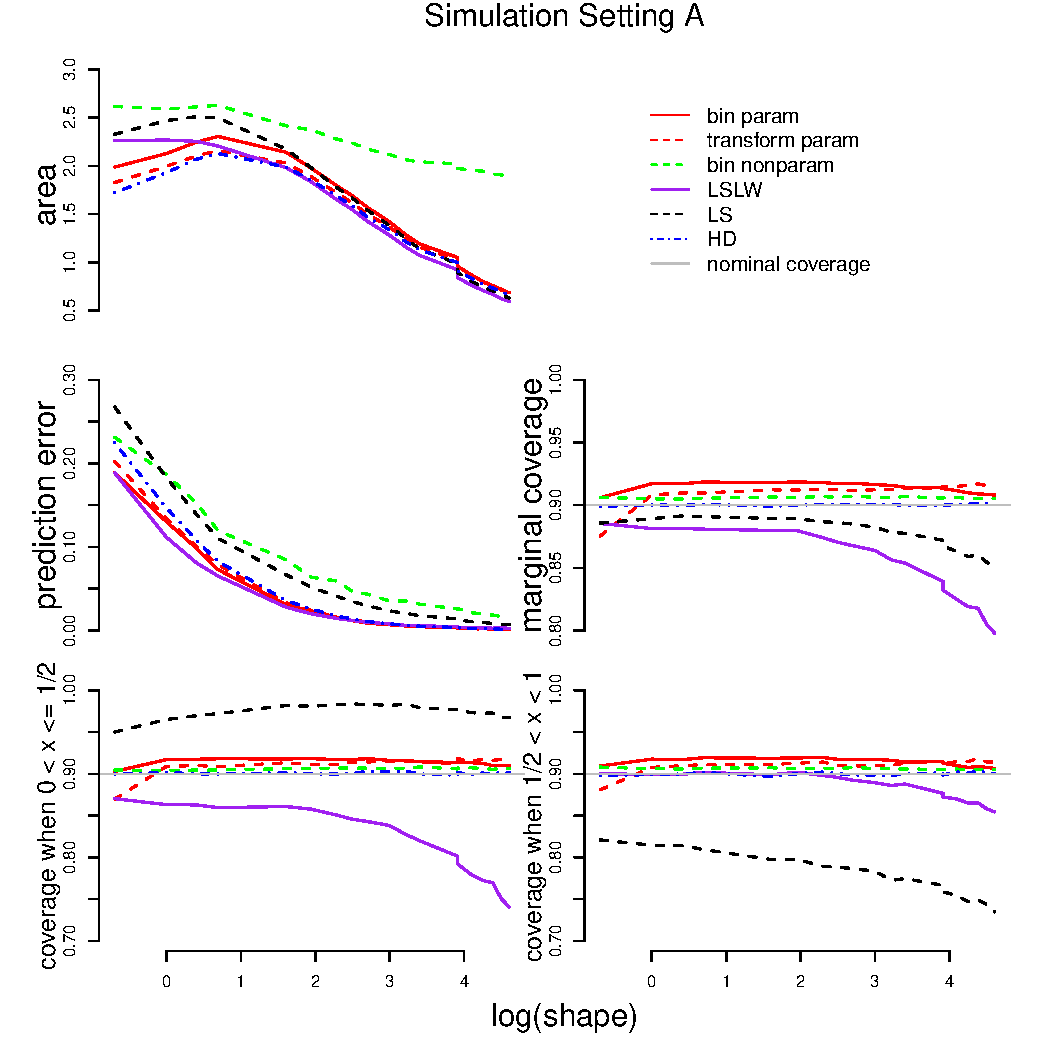
\includegraphics[width=\maxwidth]{figure/Fig-gamma-150-1} 

\end{knitrout}
\end{center}
\caption{This figure compares the performance of the 
  binned parametric,
  transformation, 
  binned nonparametric,
  least squares, and 
  least squares locally weighted conformal prediction region and the 
  highest density predcition region when $n = 150$ and the number of bins 
  equals 2.  
  The specific diagnostics used to compare these prediction regions are the 
    area,
    prediction error, 
    marginal coverage probability,
    and the coverage probability with respect to binning  
    across shape parameter values.
  The average of 200 Monte Carlo samples at each shape parameter value in 
  these simulation settings form the lines that are depicted in this figure.}
\label{Fig:gamma.150}
\end{figure}


% local coverage, n = 150
\newpage
\begin{figure}[h!]
\begin{center}
\begin{knitrout}
\definecolor{shadecolor}{rgb}{0.969, 0.969, 0.969}\color{fgcolor}
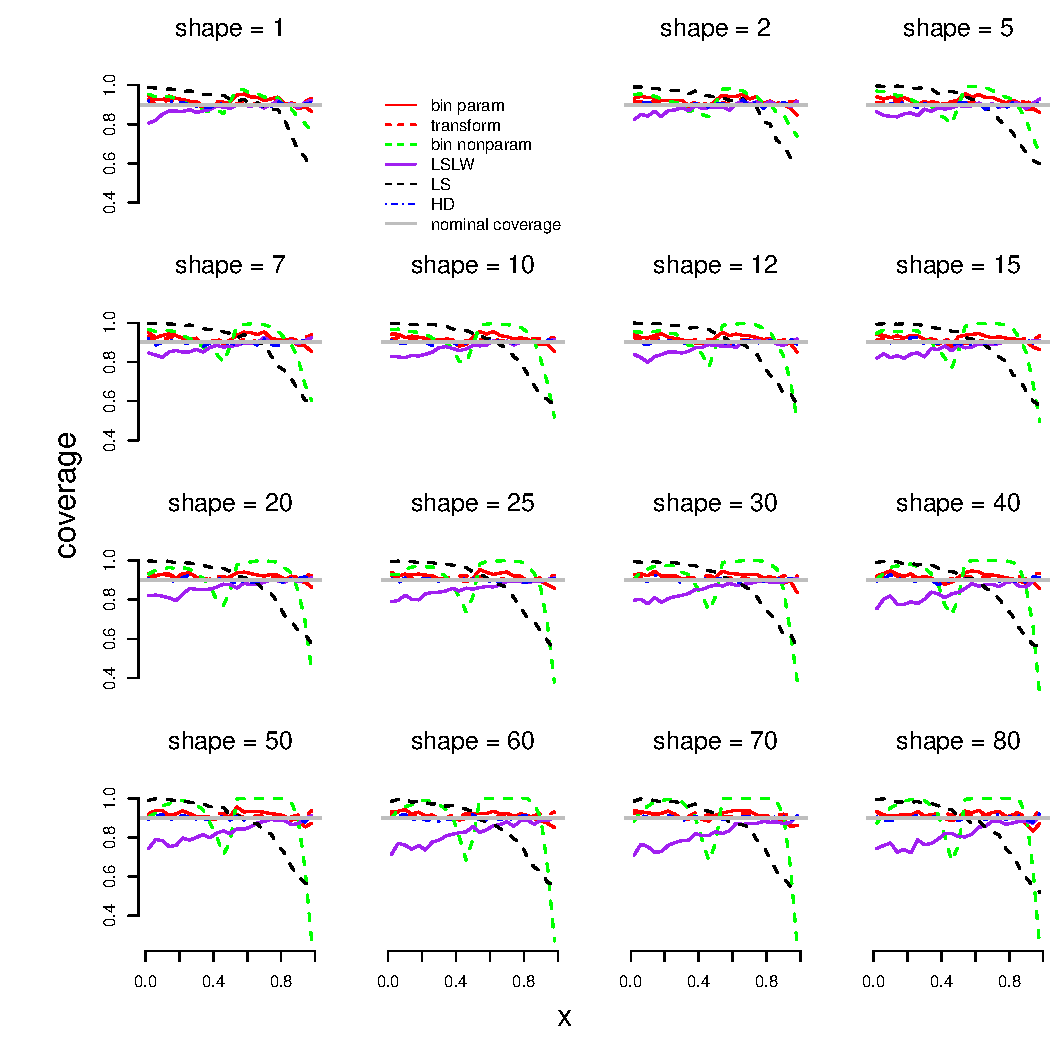
\includegraphics[width=\maxwidth]{figure/Fig-gamma-inx-150-1} 

\end{knitrout}
\end{center}
\caption{Plot of the estimated coverage probabilities of prediction regions 
  across $x$ and shape parameter values when the model is correctly 
  specified, $n = 150$, and the number of bins is equal to $2$.}
\label{Fig:gamma.inx.150}
\end{figure}


% Diagnostics, n = 250
\newpage
\begin{figure}[h!]
\begin{center}
\begin{knitrout}
\definecolor{shadecolor}{rgb}{0.969, 0.969, 0.969}\color{fgcolor}
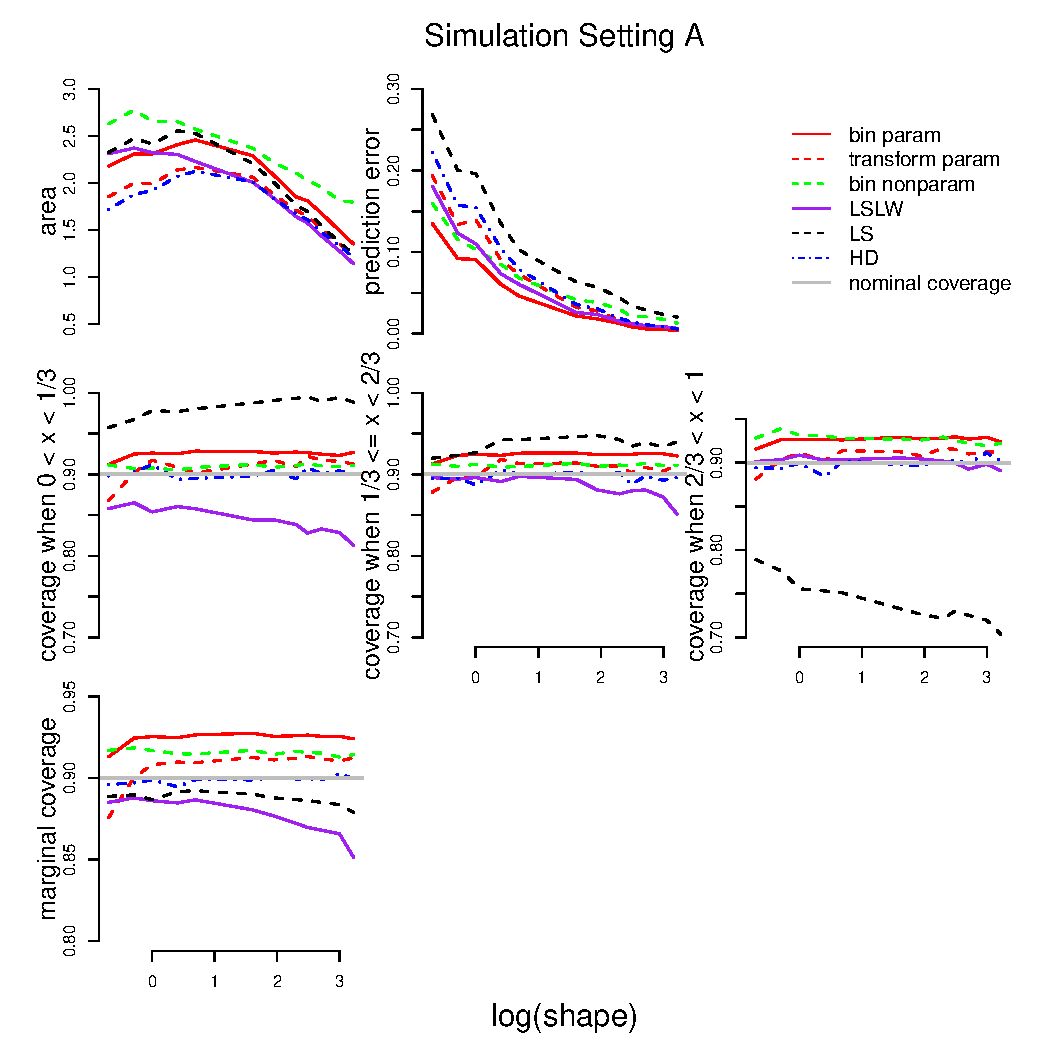
\includegraphics[width=\maxwidth]{figure/Fig-gamma-250-1} 

\end{knitrout}
\end{center}
\caption{This figure compares the performance of the 
  binned parametric,
  transformation,
  binned nonparametric,
  least squares, and 
  least squares locally weighted conformal prediction region and the 
  highest density prediction region when $n = 250$ and the number of bins 
  equals 3.  
  The specific diagnostics used to compare these prediction regions is the 
    area,
    prediction error, 
    marginal coverage probability,
    and the coverage probability with respect to binning 
    across shape parameter values.
  The average of 50 Monte Carlo samples at each shape parameter value in 
  these simulation settings form the lines that are depicted in this figure.}
\label{Fig:gamma.250}
\end{figure}



% local coverage, n = 250
\newpage
\begin{figure}[h!]
\begin{center}
\begin{knitrout}
\definecolor{shadecolor}{rgb}{0.969, 0.969, 0.969}\color{fgcolor}
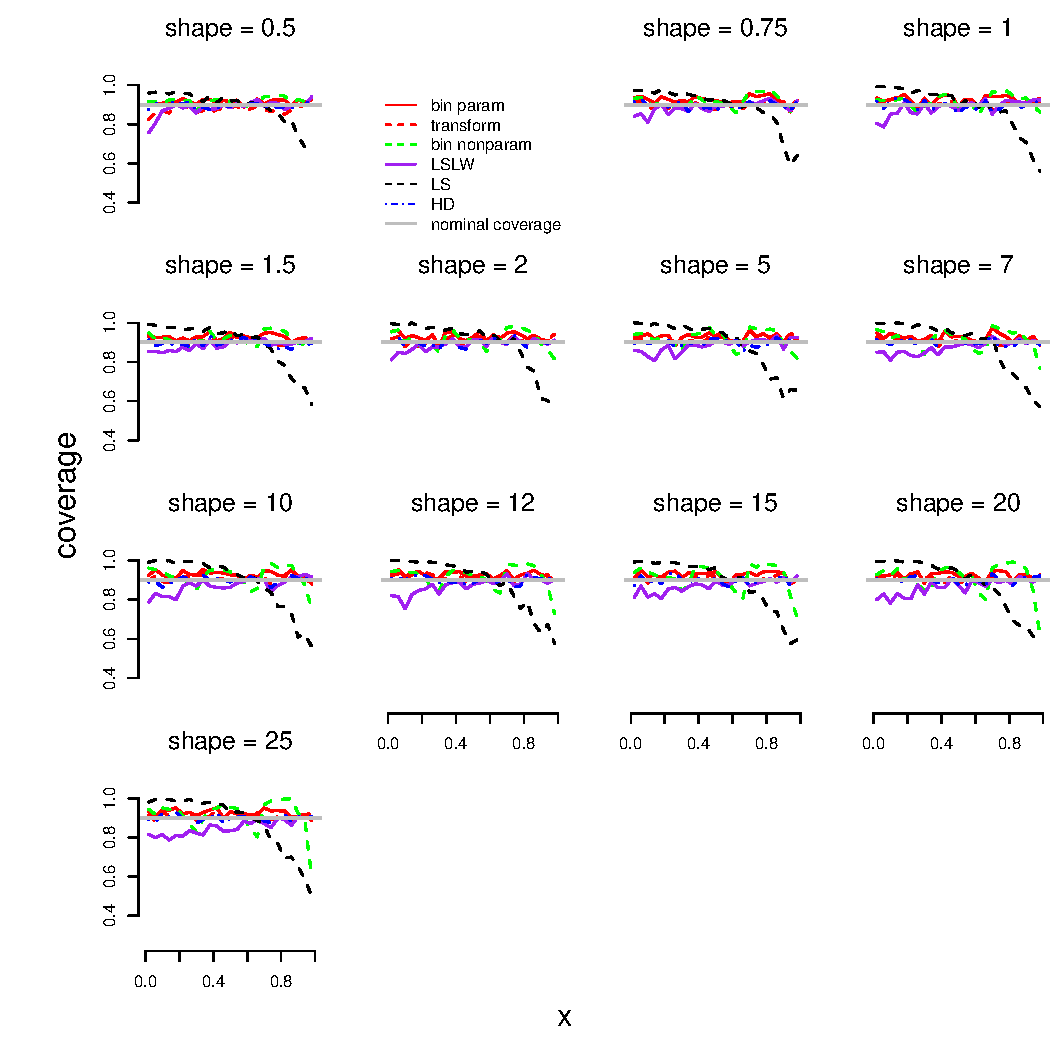
\includegraphics[width=\maxwidth]{figure/Fig-gamma-inx-250-1} 

\end{knitrout}
\end{center}
\caption{Plot of the estimated coverage probabilities of prediction regions 
  across $x$ and shape parameter values when the model is correctly 
  specified, $n = 250$, and the number of bins is equal to $3$.}
\label{Fig:gamma.inx.250}
\end{figure}



% Diagnostics, n = 500
\newpage
\begin{figure}[h!]
\begin{center}
\begin{knitrout}
\definecolor{shadecolor}{rgb}{0.969, 0.969, 0.969}\color{fgcolor}
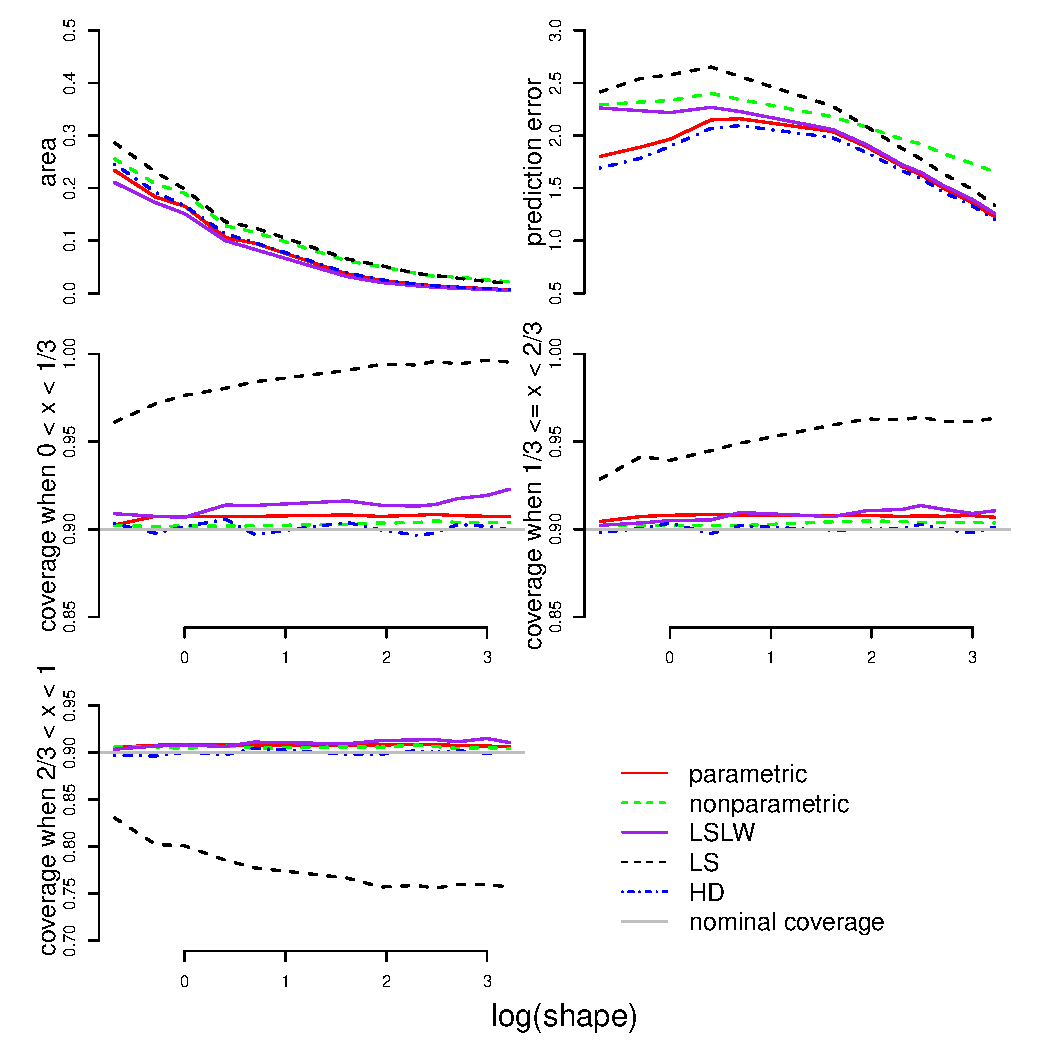
\includegraphics[width=\maxwidth]{figure/Fig-gamma-500-1} 

\end{knitrout}
\end{center}
\caption{This figure compares the performance of the 
  binned parametric,
  transformation,
  binned nonparametric,
  least squares, and 
  least squares locally weighted conformal prediction region and the 
  highest density prediction region when $n = 500$ and the number of bins 
  equals 3.  
  The specific diagnostics used to compare these prediction regions is the 
    area,
    prediction error, 
    marginal coverage probability,
    and the coverage probability with respect to binning 
    across shape parameter values.
  The average of 50 Monte Carlo samples at each shape parameter value in 
  these simulation settings form the lines that are depicted in this figure.}
\label{Fig:gamma.500}
\end{figure}



% local coverage, n = 500
\newpage
\begin{figure}[h!]
\begin{center}
\begin{knitrout}
\definecolor{shadecolor}{rgb}{0.969, 0.969, 0.969}\color{fgcolor}
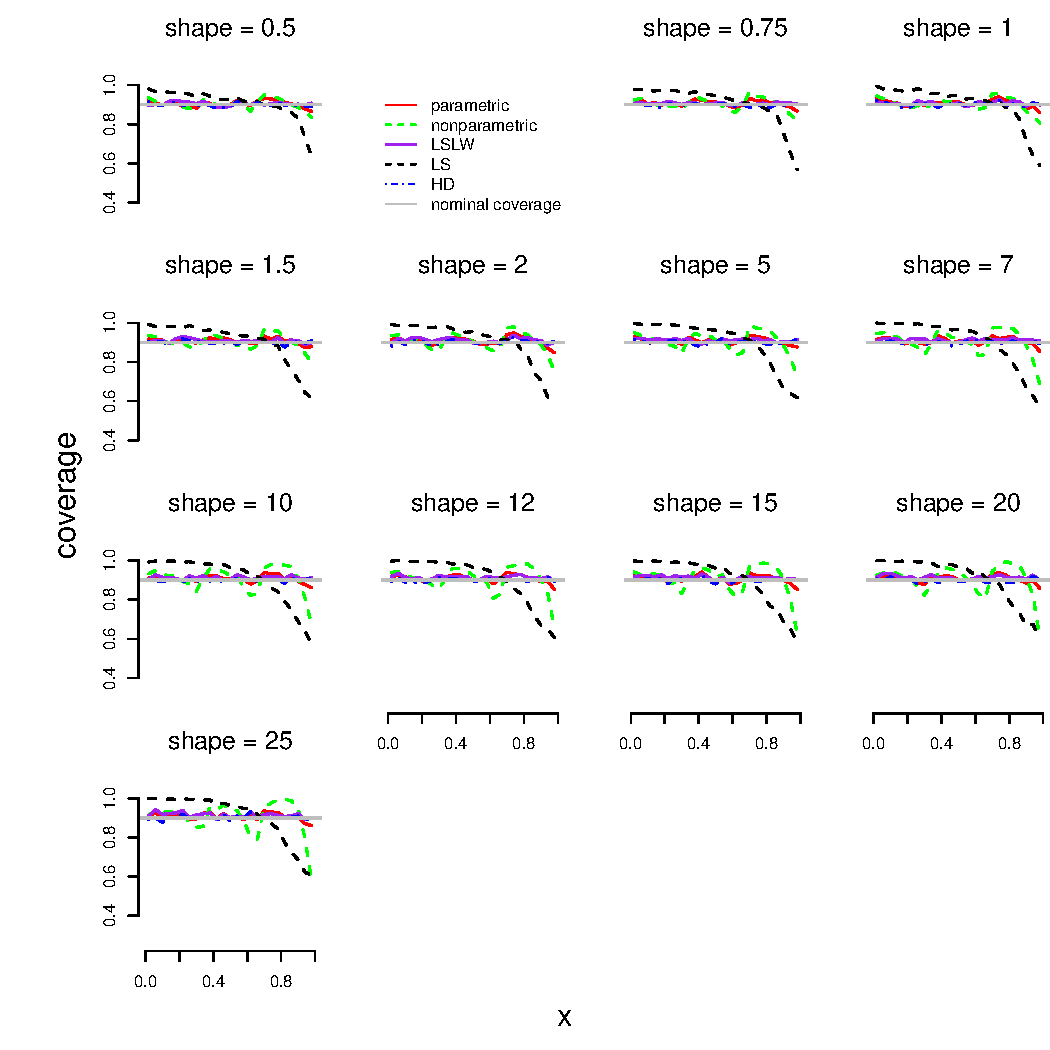
\includegraphics[width=\maxwidth]{figure/Fig-gamma-inx-500-1} 

\end{knitrout}
\end{center}
\caption{Plot of the estimated coverage probabilities of prediction regions 
  across $x$ and shape parameter values when the model is correctly 
  specified, $n = 500$, and the number of bins is equal to $3$.}
\label{Fig:gamma.inx.500}
\end{figure}







\newpage
\section{Gamma-Gaussian model misspecification}
\label{sec:misspec}

In this Section, we compare the binned parametric and nonparametric conformal 
prediction regions, the transformation based conformal prediction region, 
the LSLW conformal prediction region, the LS conformal prediction region, 
and the HD prediction region under model misspecification.  The data 
generating process is Gamma with an inverse link function and we set 
$\beta = (0.5, 1)^T$.   We consider sample sizes of $n \in \{150, 250, 500\}$ 
and shape parameter values of $\{5, 10, 20, 30, 40, 50, 60, 70, 80, 90, 100\}$ 
when $n = 150$ and shape parameter values of $\{5, 20, 40, 60, 80, 100\}$ 
when $n = 250, 500$.  This value of $\beta$ and these shape parameter values 
are chosen so that errors about a cubic regression model appear to be almost 
symmetric.  In this analysis the binned and transformation based parametric, 
LSLW, and LS conformal prediction regions are fit assuming this misspecified 
cubic regression model with homoscedastic normal errors, and the HD prediction 
region is fit to the true data generating Gamma model.  When $n = 150$ we 
build the binned parametric and nonparametric conformal prediction regions 
using 2 bins.  When $n = 250, 500$ we build the parametric and nonparametric 
conformal prediction regions using 3 bins.  These number of bin choices 
correspond to the bin width asymptotics of \citet{lei2014distribution}. 

We also compare the HD prediction region fit to the misspecified cubic 
regression model with homoscedastic normal errors when $n = 150$.  


\subsection{Simulations}

The following function computes our diagnostic measures for the six 
prediction regions under investigation in the univariate case where data 
is assumed to be Gamma with inverse link function and the fitted model is 
Gaussian with a cubic fit.  

\begin{knitrout}
\definecolor{shadecolor}{rgb}{0.969, 0.969, 0.969}\color{fgcolor}\begin{kframe}
\begin{alltt}
\hlstd{beta} \hlkwb{<-} \hlkwd{c}\hlstd{(}\hlnum{0.5}\hlstd{,} \hlnum{1}\hlstd{)}
\hlstd{misspec_simulator} \hlkwb{<-} \hlkwa{function}\hlstd{(}\hlkwc{beta}\hlstd{,} \hlkwc{n} \hlstd{=} \hlnum{150}\hlstd{,} \hlkwc{shape} \hlstd{=} \hlnum{0.5}\hlstd{,}
  \hlkwc{bins} \hlstd{=} \hlnum{2}\hlstd{,} \hlkwc{alpha} \hlstd{=} \hlnum{0.10}\hlstd{,} \hlkwc{B} \hlstd{=} \hlnum{2}\hlstd{)\{}

  \hlstd{p} \hlkwb{<-} \hlstd{d} \hlkwb{<-} \hlkwd{length}\hlstd{(beta)} \hlopt{-} \hlnum{1}

  \hlstd{models} \hlkwb{<-} \hlkwd{lapply}\hlstd{(}\hlnum{1}\hlopt{:}\hlstd{B,} \hlkwc{FUN} \hlstd{=} \hlkwa{function}\hlstd{(}\hlkwc{j}\hlstd{)\{}
    \hlstd{x} \hlkwb{<-} \hlkwd{matrix}\hlstd{(}\hlkwd{runif}\hlstd{(n}\hlopt{*}\hlstd{p),} \hlkwc{ncol} \hlstd{= p)}
    \hlstd{rate} \hlkwb{<-} \hlstd{(}\hlkwd{cbind}\hlstd{(}\hlnum{1}\hlstd{, x)} \hlopt \hlstd{beta)} \hlopt{*} \hlstd{shape}
    \hlstd{y} \hlkwb{<-} \hlkwd{rgamma}\hlstd{(}\hlkwc{n} \hlstd{= n,} \hlkwc{shape} \hlstd{= shape,} \hlkwc{rate} \hlstd{= rate)}
    \hlstd{y} \hlkwb{<-} \hlstd{y} \hlopt{/} \hlkwd{sd}\hlstd{(y)}
    \hlstd{dat} \hlkwb{<-} \hlkwd{data.frame}\hlstd{(}\hlkwc{y} \hlstd{= y,} \hlkwc{x} \hlstd{= x)}
    \hlkwd{colnames}\hlstd{(dat)[}\hlnum{2}\hlopt{:}\hlstd{(p}\hlopt{+}\hlnum{1}\hlstd{)]} \hlkwb{<-} \hlkwd{paste}\hlstd{(}\hlstr{"x"}\hlstd{,} \hlnum{1}\hlopt{:}\hlstd{p,} \hlkwc{sep} \hlstd{=} \hlstr{""}\hlstd{)}
    \hlstd{fit} \hlkwb{<-} \hlkwd{glm}\hlstd{(y} \hlopt{~} \hlstd{x1} \hlopt{+} \hlkwd{I}\hlstd{(x1}\hlopt{^}\hlnum{2}\hlstd{)} \hlopt{+} \hlkwd{I}\hlstd{(x1}\hlopt{^}\hlnum{3}\hlstd{),} \hlkwc{family} \hlstd{=} \hlstr{"gaussian"}\hlstd{,}
      \hlkwc{data} \hlstd{= dat,} \hlkwc{x} \hlstd{=} \hlnum{TRUE}\hlstd{,} \hlkwc{y} \hlstd{=} \hlnum{TRUE}\hlstd{)}
    \hlstd{fit.true} \hlkwb{<-} \hlkwd{glm}\hlstd{(y} \hlopt{~} \hlstd{x1,} \hlkwc{family} \hlstd{=} \hlstr{"Gamma"}\hlstd{,}
      \hlkwc{data} \hlstd{= dat,} \hlkwc{x} \hlstd{=} \hlnum{TRUE}\hlstd{,} \hlkwc{y} \hlstd{=} \hlnum{TRUE}\hlstd{)}
    \hlstd{output} \hlkwb{=} \hlkwd{list}\hlstd{(}\hlkwc{model} \hlstd{= fit,} \hlkwc{model.true} \hlstd{= fit.true,} \hlkwc{dat} \hlstd{= dat)}
    \hlstd{output}
  \hlstd{\})}

  \hlstd{funs} \hlkwb{<-} \hlkwd{lm.funs}\hlstd{(}\hlkwc{intercept} \hlstd{=} \hlnum{TRUE}\hlstd{)}
  \hlstd{train.fun} \hlkwb{<-} \hlstd{funs}\hlopt{$}\hlstd{train.fun}
  \hlstd{predict.fun} \hlkwb{<-} \hlstd{funs}\hlopt{$}\hlstd{predict.fun}
  \hlstd{conformal_regions} \hlkwb{<-} \hlkwd{lapply}\hlstd{(models,} \hlkwc{FUN} \hlstd{=} \hlkwa{function}\hlstd{(}\hlkwc{obj}\hlstd{)\{}

    \hlstd{model} \hlkwb{<-} \hlstd{obj}\hlopt{$}\hlstd{model}
    \hlstd{dat} \hlkwb{<-} \hlstd{obj}\hlopt{$}\hlstd{dat}
    \hlstd{model}\hlopt{$}\hlstd{data} \hlkwb{<-} \hlstd{dat}
    \hlstd{x} \hlkwb{<-} \hlstd{model}\hlopt{$}\hlstd{x[,} \hlnum{2}\hlstd{]}
    \hlstd{y} \hlkwb{<-} \hlstd{model}\hlopt{$}\hlstd{y}
    \hlstd{p1.tibs} \hlkwb{<-} \hlkwd{conformal.pred}\hlstd{(}\hlkwc{x} \hlstd{=} \hlkwd{cbind}\hlstd{(x,x}\hlopt{^}\hlnum{2}\hlstd{,x}\hlopt{^}\hlnum{3}\hlstd{),} \hlkwc{y} \hlstd{= y,}
      \hlkwc{x0} \hlstd{=} \hlkwd{cbind}\hlstd{(x,x}\hlopt{^}\hlnum{2}\hlstd{,x}\hlopt{^}\hlnum{3}\hlstd{),}
      \hlkwc{train.fun} \hlstd{= train.fun,} \hlkwc{predict.fun} \hlstd{= predict.fun,}
      \hlkwc{alpha} \hlstd{= alpha)}
    \hlstd{LSCI} \hlkwb{<-} \hlkwd{cbind}\hlstd{(p1.tibs}\hlopt{$}\hlstd{lo, p1.tibs}\hlopt{$}\hlstd{up)}

    \hlstd{cubic.model} \hlkwb{<-} \hlkwd{lm}\hlstd{(y} \hlopt{~} \hlstd{x} \hlopt{+} \hlkwd{I}\hlstd{(x}\hlopt{^}\hlnum{2}\hlstd{)} \hlopt{+} \hlkwd{I}\hlstd{(x}\hlopt{^}\hlnum{3}\hlstd{))}
    \hlstd{abs.resid} \hlkwb{<-} \hlkwd{abs}\hlstd{(cubic.model}\hlopt{$}\hlstd{resid)}
    \hlstd{smooth.call} \hlkwb{<-} \hlkwd{smooth.spline}\hlstd{(x, abs.resid,}
      \hlkwc{nknots} \hlstd{=} \hlnum{10}\hlstd{)}
    \hlstd{lambda} \hlkwb{<-} \hlstd{smooth.call}\hlopt{$}\hlstd{lambda}
    \hlstd{df} \hlkwb{<-} \hlstd{smooth.call}\hlopt{$}\hlstd{df}
    \hlstd{mad.train.fun} \hlkwb{<-} \hlkwa{function}\hlstd{(}\hlkwc{x}\hlstd{,} \hlkwc{y}\hlstd{,} \hlkwc{out} \hlstd{=} \hlkwa{NULL}\hlstd{)\{}
      \hlkwd{smooth.spline}\hlstd{(x[,} \hlnum{1}\hlstd{], y,} \hlkwc{lambda} \hlstd{= lambda,}
      \hlkwc{df} \hlstd{= df,} \hlkwc{nknots} \hlstd{=} \hlnum{10}\hlstd{)}
    \hlstd{\}}
    \hlstd{mad.predict.fun} \hlkwb{<-} \hlkwa{function}\hlstd{(}\hlkwc{out}\hlstd{,} \hlkwc{newx}\hlstd{)\{}
      \hlkwd{predict}\hlstd{(out,} \hlkwd{as.data.frame}\hlstd{(newx))}\hlopt{$}\hlstd{y[,} \hlnum{1}\hlstd{]}
    \hlstd{\}}
    \hlstd{p2.tibs} \hlkwb{<-} \hlkwd{conformal.pred}\hlstd{(}\hlkwc{x} \hlstd{=} \hlkwd{cbind}\hlstd{(x,x}\hlopt{^}\hlnum{2}\hlstd{,x}\hlopt{^}\hlnum{3}\hlstd{),} \hlkwc{y} \hlstd{= y,}
      \hlkwc{x0} \hlstd{=} \hlkwd{cbind}\hlstd{(x,x}\hlopt{^}\hlnum{2}\hlstd{,x}\hlopt{^}\hlnum{3}\hlstd{),}
      \hlkwc{train.fun} \hlstd{= train.fun,} \hlkwc{predict.fun} \hlstd{= predict.fun,}
      \hlkwc{mad.train.fun} \hlstd{= mad.train.fun,}
      \hlkwc{mad.predict.fun} \hlstd{= mad.predict.fun,}
      \hlkwc{alpha} \hlstd{= alpha)}
    \hlstd{LSLWCI} \hlkwb{<-} \hlkwd{cbind}\hlstd{(p2.tibs}\hlopt{$}\hlstd{lo, p2.tibs}\hlopt{$}\hlstd{up)}

    \hlstd{fit.int} \hlkwb{=} \hlkwd{lm}\hlstd{(y} \hlopt{~} \hlstd{x1} \hlopt{+} \hlkwd{I}\hlstd{(x1}\hlopt{^}\hlnum{2}\hlstd{)} \hlopt{+} \hlkwd{I}\hlstd{(x1}\hlopt{^}\hlnum{3}\hlstd{),} \hlkwc{data} \hlstd{= dat)}
    \hlstd{betaMLE} \hlkwb{<-} \hlkwd{coefficients}\hlstd{(fit.int)}
    \hlstd{sdMLE} \hlkwb{<-} \hlkwd{summary}\hlstd{(fit.int)}\hlopt{$}\hlstd{sigma}
    \hlstd{meanMLE} \hlkwb{<-} \hlkwd{as.numeric}\hlstd{(}\hlkwd{cbind}\hlstd{(}\hlnum{1}\hlstd{, x, x}\hlopt{^}\hlnum{2}\hlstd{, x}\hlopt{^}\hlnum{3}\hlstd{)} \hlopt \hlstd{betaMLE)}
    \hlstd{HDCI} \hlkwb{<-} \hlkwd{do.call}\hlstd{(rbind,} \hlkwd{lapply}\hlstd{(}\hlnum{1}\hlopt{:}\hlstd{n,} \hlkwa{function}\hlstd{(}\hlkwc{j}\hlstd{)\{}
      \hlkwd{hdi}\hlstd{(qnorm,} \hlnum{1} \hlopt{-} \hlstd{alpha,} \hlkwc{mean} \hlstd{= meanMLE[j],} \hlkwc{sd} \hlstd{= sdMLE)}
    \hlstd{\}))}

    \hlstd{model.true} \hlkwb{<-} \hlstd{obj}\hlopt{$}\hlstd{model.true}
    \hlstd{betaMLE.true} \hlkwb{<-} \hlkwd{coefficients}\hlstd{(model.true)}
    \hlstd{shapeMLE.true} \hlkwb{<-} \hlkwd{as.numeric}\hlstd{(}\hlkwd{gamma.shape}\hlstd{(model.true)[}\hlnum{1}\hlstd{])}
    \hlstd{rateMLE.true} \hlkwb{<-} \hlkwd{cbind}\hlstd{(}\hlnum{1}\hlstd{, x)} \hlopt \hlstd{betaMLE.true} \hlopt{*} \hlstd{shapeMLE.true}
    \hlstd{HDCI.true} \hlkwb{<-} \hlkwd{do.call}\hlstd{(rbind,} \hlkwd{lapply}\hlstd{(}\hlnum{1}\hlopt{:}\hlstd{n,} \hlkwa{function}\hlstd{(}\hlkwc{j}\hlstd{)\{}
      \hlkwd{hdi}\hlstd{(qgamma,} \hlnum{1} \hlopt{-} \hlstd{alpha,} \hlkwc{shape} \hlstd{= shapeMLE.true,} \hlkwc{rate} \hlstd{= rateMLE.true[j,} \hlnum{1}\hlstd{])}
    \hlstd{\}))}

    \hlstd{conf} \hlkwb{<-} \hlkwd{conformal.glm}\hlstd{(model,} \hlkwc{nonparametric} \hlstd{=} \hlnum{TRUE}\hlstd{,} \hlkwc{method} \hlstd{=} \hlstr{"both"}\hlstd{,}
      \hlkwc{bins} \hlstd{= bins,} \hlkwc{cores} \hlstd{=} \hlnum{7}\hlstd{)}
    \hlstd{parabinCI} \hlkwb{<-} \hlstd{conf}\hlopt{$}\hlstd{paraconfbin}
    \hlstd{transformCI} \hlkwb{<-} \hlstd{conf}\hlopt{$}\hlstd{transformconf}
    \hlstd{nonparabinCI} \hlkwb{<-} \hlstd{conf}\hlopt{$}\hlstd{nonparaconfbin}

    \hlstd{out} \hlkwb{=} \hlkwd{list}\hlstd{(}\hlkwc{parabinCI} \hlstd{= parabinCI,} \hlkwc{transformCI} \hlstd{= transformCI,}
      \hlkwc{nonparabinCI} \hlstd{= nonparabinCI,} \hlkwc{LSLWCI} \hlstd{= LSLWCI,} \hlkwc{LSCI} \hlstd{= LSCI,}
      \hlkwc{HDCI} \hlstd{= HDCI,} \hlkwc{HDCI.true} \hlstd{= HDCI.true)}
    \hlstd{out}
  \hlstd{\})}

  \hlstd{diagnostics_regions} \hlkwb{<-} \hlkwd{lapply}\hlstd{(}\hlnum{1}\hlopt{:}\hlstd{B,} \hlkwc{FUN} \hlstd{=} \hlkwa{function}\hlstd{(}\hlkwc{j}\hlstd{)\{}

    \hlstd{obj} \hlkwb{<-} \hlstd{conformal_regions[[j]]}
    \hlstd{dat} \hlkwb{<-} \hlkwd{as.data.frame}\hlstd{(models[[j]]}\hlopt{$}\hlstd{dat)}
    \hlstd{y} \hlkwb{<-} \hlkwd{as.numeric}\hlstd{(dat[,} \hlnum{1}\hlstd{])}

    \hlstd{diagnostics} \hlkwb{<-} \hlkwd{lapply}\hlstd{(obj,} \hlkwc{FUN} \hlstd{=} \hlkwa{function}\hlstd{(}\hlkwc{region}\hlstd{)\{}

      \hlstd{output} \hlkwb{<-} \hlkwa{NULL}
      \hlkwa{if}\hlstd{(}\hlkwd{class}\hlstd{(region)} \hlopt{==} \hlstr{"matrix"}\hlstd{)\{}
        \hlstd{marginal.coverage} \hlkwb{<-} \hlkwd{local.coverage}\hlstd{(}\hlkwc{region} \hlstd{= region,}
          \hlkwc{data} \hlstd{= dat,} \hlkwc{d} \hlstd{= p,} \hlkwc{bins} \hlstd{=} \hlnum{1}\hlstd{,} \hlkwc{at.data} \hlstd{=} \hlstr{"TRUE"}\hlstd{)}
        \hlstd{local.coverage} \hlkwb{<-} \hlkwd{local.coverage}\hlstd{(}\hlkwc{region} \hlstd{= region,}
          \hlkwc{data} \hlstd{= dat,} \hlkwc{d} \hlstd{= p,} \hlkwc{bins} \hlstd{= bins,} \hlkwc{at.data} \hlstd{=} \hlstr{"TRUE"}\hlstd{)}
        \hlstd{local.inx.coverage} \hlkwb{<-} \hlkwd{local.coverage}\hlstd{(}\hlkwc{region} \hlstd{= region,}
          \hlkwc{data} \hlstd{= dat,} \hlkwc{d} \hlstd{= p,} \hlkwc{bins} \hlstd{=} \hlnum{25}\hlstd{,} \hlkwc{at.data} \hlstd{=} \hlstr{"TRUE"}\hlstd{)}
        \hlstd{output} \hlkwb{<-} \hlkwd{c}\hlstd{(marginal.coverage, local.coverage,}
          \hlstd{local.inx.coverage,} \hlkwd{mean}\hlstd{(}\hlkwd{apply}\hlstd{(region,} \hlnum{1}\hlstd{, diff)),}
          \hlkwd{absolute.error}\hlstd{(}\hlkwc{y} \hlstd{= y,} \hlkwc{region} \hlstd{= region))}
      \hlstd{\}}
      \hlkwa{else}\hlstd{\{}
        \hlstd{marginal.coverage} \hlkwb{<-} \hlkwd{local.coverage}\hlstd{(}\hlkwc{region} \hlstd{= region,}
          \hlkwc{nonparametric} \hlstd{=} \hlstr{"TRUE"}\hlstd{,} \hlkwc{data} \hlstd{= dat,} \hlkwc{d} \hlstd{= p,} \hlkwc{bins} \hlstd{=} \hlnum{1}\hlstd{,}
          \hlkwc{at.data} \hlstd{=} \hlstr{"TRUE"}\hlstd{)}
        \hlstd{local.coverage} \hlkwb{<-} \hlkwd{local.coverage}\hlstd{(}\hlkwc{region} \hlstd{= region,}
          \hlkwc{nonparametric} \hlstd{=} \hlstr{"TRUE"}\hlstd{,} \hlkwc{data} \hlstd{= dat,} \hlkwc{d} \hlstd{= p,} \hlkwc{bins} \hlstd{= bins,}
          \hlkwc{at.data} \hlstd{=} \hlstr{"TRUE"}\hlstd{)}
        \hlstd{local.inx.coverage} \hlkwb{<-} \hlkwd{local.coverage}\hlstd{(}\hlkwc{region} \hlstd{= region,}
          \hlkwc{nonparametric} \hlstd{=} \hlstr{"TRUE"}\hlstd{,} \hlkwc{data} \hlstd{= dat,} \hlkwc{d} \hlstd{= p,} \hlkwc{bins} \hlstd{=} \hlnum{25}\hlstd{,}
          \hlkwc{at.data} \hlstd{=} \hlstr{"TRUE"}\hlstd{)}
        \hlstd{output} \hlkwb{<-} \hlkwd{c}\hlstd{(marginal.coverage, local.coverage,}
          \hlstd{local.inx.coverage,} \hlkwd{area.nonparametric}\hlstd{(region),}
          \hlkwd{absolute.error.nonparametric}\hlstd{(}\hlkwc{data} \hlstd{= dat,}
            \hlkwc{region} \hlstd{= region))}
      \hlstd{\}}
      \hlstd{output}
    \hlstd{\})}
    \hlkwd{do.call}\hlstd{(rbind, diagnostics)}

  \hlstd{\})}

  \hlstd{diagnostics_regions}
\hlstd{\}}
\end{alltt}
\end{kframe}
\end{knitrout}



The following performs our Monte Carlo simulation of $B = 200$ iterations 
when $n = 150$ and shape = $0.75$.

\begin{knitrout}
\definecolor{shadecolor}{rgb}{0.969, 0.969, 0.969}\color{fgcolor}\begin{kframe}
\begin{alltt}
\hlkwd{set.seed}\hlstd{(}\hlnum{13}\hlstd{)}
\hlstd{n} \hlkwb{<-} \hlnum{150}
\hlstd{bins} \hlkwb{<-} \hlnum{2}
\hlstd{B} \hlkwb{<-} \hlnum{200}
\hlkwd{system.time}\hlstd{(out.misspec.150.2.0.75} \hlkwb{<-} \hlkwd{do.call}\hlstd{(rbind,}
  \hlkwd{misspec_simulator}\hlstd{(}\hlkwc{beta} \hlstd{= beta,} \hlkwc{n} \hlstd{= n,} \hlkwc{shape} \hlstd{=} \hlnum{0.75}\hlstd{,} \hlkwc{bins} \hlstd{= bins,} \hlkwc{B} \hlstd{= B)))}
\end{alltt}
\begin{verbatim}
##      user    system   elapsed 
## 18259.601   226.217  7293.052
\end{verbatim}
\begin{alltt}
\hlstd{diagnostics.misspec.150.2.0.75} \hlkwb{<-} \hlkwd{do.call}\hlstd{(rbind,} \hlkwd{lapply}\hlstd{(}\hlkwd{split}\hlstd{(out.misspec.150.2.0.75,}
  \hlkwc{f} \hlstd{=} \hlkwd{as.factor}\hlstd{(}\hlkwd{rownames}\hlstd{(out.misspec.150.2.0.75))),}
  \hlkwc{FUN} \hlstd{=} \hlkwa{function}\hlstd{(}\hlkwc{xx}\hlstd{)} \hlkwd{colMeans}\hlstd{(}\hlkwd{matrix}\hlstd{(xx,} \hlkwc{nrow} \hlstd{= B),} \hlkwc{na.rm} \hlstd{=} \hlnum{TRUE}\hlstd{)))}
\end{alltt}
\end{kframe}
\end{knitrout}


The following performs our Monte Carlo simulation of $B = 200$ iterations 
when $n = 150$ and shape = $1$.

\begin{knitrout}
\definecolor{shadecolor}{rgb}{0.969, 0.969, 0.969}\color{fgcolor}\begin{kframe}
\begin{alltt}
\hlkwd{set.seed}\hlstd{(}\hlnum{13}\hlstd{)}
\hlkwd{system.time}\hlstd{(out.misspec.150.2.1} \hlkwb{<-} \hlkwd{do.call}\hlstd{(rbind,}
  \hlkwd{misspec_simulator}\hlstd{(}\hlkwc{beta} \hlstd{= beta,} \hlkwc{n} \hlstd{= n,} \hlkwc{shape} \hlstd{=} \hlnum{1}\hlstd{,} \hlkwc{bins} \hlstd{= bins,} \hlkwc{B} \hlstd{= B)))}
\end{alltt}
\begin{verbatim}
##      user    system   elapsed 
## 17689.076   216.942  7207.307
\end{verbatim}
\begin{alltt}
\hlstd{diagnostics.misspec.150.2.1} \hlkwb{<-} \hlkwd{do.call}\hlstd{(rbind,} \hlkwd{lapply}\hlstd{(}\hlkwd{split}\hlstd{(out.misspec.150.2.1,}
  \hlkwc{f} \hlstd{=} \hlkwd{as.factor}\hlstd{(}\hlkwd{rownames}\hlstd{(out.misspec.150.2.1))),}
  \hlkwc{FUN} \hlstd{=} \hlkwa{function}\hlstd{(}\hlkwc{xx}\hlstd{)} \hlkwd{colMeans}\hlstd{(}\hlkwd{matrix}\hlstd{(xx,} \hlkwc{nrow} \hlstd{= B),} \hlkwc{na.rm} \hlstd{=} \hlnum{TRUE}\hlstd{)))}
\end{alltt}
\end{kframe}
\end{knitrout}


The following performs our Monte Carlo simulation of $B = 200$ iterations 
when $n = 150$ and shape = $2$.

\begin{knitrout}
\definecolor{shadecolor}{rgb}{0.969, 0.969, 0.969}\color{fgcolor}\begin{kframe}
\begin{alltt}
\hlkwd{set.seed}\hlstd{(}\hlnum{13}\hlstd{)}
\hlkwd{system.time}\hlstd{(out.misspec.150.2.2} \hlkwb{<-} \hlkwd{do.call}\hlstd{(rbind,}
  \hlkwd{misspec_simulator}\hlstd{(}\hlkwc{beta} \hlstd{= beta,} \hlkwc{n} \hlstd{= n,} \hlkwc{shape} \hlstd{=} \hlnum{2}\hlstd{,} \hlkwc{bins} \hlstd{= bins,} \hlkwc{B} \hlstd{= B)))}
\end{alltt}
\begin{verbatim}
##      user    system   elapsed 
## 17933.057   248.811  7260.141
\end{verbatim}
\begin{alltt}
\hlstd{diagnostics.misspec.150.2.2} \hlkwb{<-} \hlkwd{do.call}\hlstd{(rbind,} \hlkwd{lapply}\hlstd{(}\hlkwd{split}\hlstd{(out.misspec.150.2.2,}
  \hlkwc{f} \hlstd{=} \hlkwd{as.factor}\hlstd{(}\hlkwd{rownames}\hlstd{(out.misspec.150.2.2))),}
  \hlkwc{FUN} \hlstd{=} \hlkwa{function}\hlstd{(}\hlkwc{xx}\hlstd{)} \hlkwd{colMeans}\hlstd{(}\hlkwd{matrix}\hlstd{(xx,} \hlkwc{nrow} \hlstd{= B),} \hlkwc{na.rm} \hlstd{=} \hlnum{TRUE}\hlstd{)))}
\end{alltt}
\end{kframe}
\end{knitrout}


The following performs our Monte Carlo simulation of $B = 200$ iterations 
when $n = 150$ and shape = $5$.

\begin{knitrout}
\definecolor{shadecolor}{rgb}{0.969, 0.969, 0.969}\color{fgcolor}\begin{kframe}
\begin{alltt}
\hlkwd{set.seed}\hlstd{(}\hlnum{13}\hlstd{)}
\hlkwd{system.time}\hlstd{(out.misspec.150.2.5} \hlkwb{<-} \hlkwd{do.call}\hlstd{(rbind,}
  \hlkwd{misspec_simulator}\hlstd{(}\hlkwc{beta} \hlstd{= beta,} \hlkwc{n} \hlstd{= n,} \hlkwc{shape} \hlstd{=} \hlnum{5}\hlstd{,} \hlkwc{bins} \hlstd{= bins,} \hlkwc{B} \hlstd{= B)))}
\end{alltt}
\begin{verbatim}
##      user    system   elapsed 
## 17262.546   226.816  7170.114
\end{verbatim}
\begin{alltt}
\hlstd{diagnostics.misspec.150.2.5} \hlkwb{<-} \hlkwd{do.call}\hlstd{(rbind,} \hlkwd{lapply}\hlstd{(}\hlkwd{split}\hlstd{(out.misspec.150.2.5,}
  \hlkwc{f} \hlstd{=} \hlkwd{as.factor}\hlstd{(}\hlkwd{rownames}\hlstd{(out.misspec.150.2.5))),}
  \hlkwc{FUN} \hlstd{=} \hlkwa{function}\hlstd{(}\hlkwc{xx}\hlstd{)} \hlkwd{colMeans}\hlstd{(}\hlkwd{matrix}\hlstd{(xx,} \hlkwc{nrow} \hlstd{= B),} \hlkwc{na.rm} \hlstd{=} \hlnum{TRUE}\hlstd{)))}
\end{alltt}
\end{kframe}
\end{knitrout}


The following performs our Monte Carlo simulation of $B = 200$ iterations 
when $n = 150$ and shape = $7$.

\begin{knitrout}
\definecolor{shadecolor}{rgb}{0.969, 0.969, 0.969}\color{fgcolor}\begin{kframe}
\begin{alltt}
\hlkwd{set.seed}\hlstd{(}\hlnum{13}\hlstd{)}
\hlkwd{system.time}\hlstd{(out.misspec.150.2.7} \hlkwb{<-} \hlkwd{do.call}\hlstd{(rbind,}
  \hlkwd{misspec_simulator}\hlstd{(}\hlkwc{beta} \hlstd{= beta,} \hlkwc{n} \hlstd{= n,} \hlkwc{shape} \hlstd{=} \hlnum{7}\hlstd{,} \hlkwc{bins} \hlstd{= bins,} \hlkwc{B} \hlstd{= B)))}
\end{alltt}
\begin{verbatim}
##      user    system   elapsed 
## 16908.723   228.178  7103.159
\end{verbatim}
\begin{alltt}
\hlstd{diagnostics.misspec.150.2.7} \hlkwb{<-} \hlkwd{do.call}\hlstd{(rbind,} \hlkwd{lapply}\hlstd{(}\hlkwd{split}\hlstd{(out.misspec.150.2.7,}
  \hlkwc{f} \hlstd{=} \hlkwd{as.factor}\hlstd{(}\hlkwd{rownames}\hlstd{(out.misspec.150.2.7))),}
  \hlkwc{FUN} \hlstd{=} \hlkwa{function}\hlstd{(}\hlkwc{xx}\hlstd{)} \hlkwd{colMeans}\hlstd{(}\hlkwd{matrix}\hlstd{(xx,} \hlkwc{nrow} \hlstd{= B),} \hlkwc{na.rm} \hlstd{=} \hlnum{TRUE}\hlstd{)))}
\end{alltt}
\end{kframe}
\end{knitrout}


The following performs our Monte Carlo simulation of $B = 200$ iterations 
when $n = 150$ and shape = $10$.

\begin{knitrout}
\definecolor{shadecolor}{rgb}{0.969, 0.969, 0.969}\color{fgcolor}\begin{kframe}
\begin{alltt}
\hlkwd{set.seed}\hlstd{(}\hlnum{13}\hlstd{)}
\hlkwd{system.time}\hlstd{(out.misspec.150.2.10} \hlkwb{<-} \hlkwd{do.call}\hlstd{(rbind,}
  \hlkwd{misspec_simulator}\hlstd{(}\hlkwc{beta} \hlstd{= beta,} \hlkwc{n} \hlstd{= n,} \hlkwc{shape} \hlstd{=} \hlnum{10}\hlstd{,} \hlkwc{bins} \hlstd{= bins,} \hlkwc{B} \hlstd{= B)))}
\end{alltt}
\begin{verbatim}
##      user    system   elapsed 
## 16080.013   234.080  6976.448
\end{verbatim}
\begin{alltt}
\hlstd{diagnostics.misspec.150.2.10} \hlkwb{<-} \hlkwd{do.call}\hlstd{(rbind,} \hlkwd{lapply}\hlstd{(}\hlkwd{split}\hlstd{(out.misspec.150.2.10,}
  \hlkwc{f} \hlstd{=} \hlkwd{as.factor}\hlstd{(}\hlkwd{rownames}\hlstd{(out.misspec.150.2.10))),}
  \hlkwc{FUN} \hlstd{=} \hlkwa{function}\hlstd{(}\hlkwc{xx}\hlstd{)} \hlkwd{colMeans}\hlstd{(}\hlkwd{matrix}\hlstd{(xx,} \hlkwc{nrow} \hlstd{= B),} \hlkwc{na.rm} \hlstd{=} \hlnum{TRUE}\hlstd{)))}
\end{alltt}
\end{kframe}
\end{knitrout}


The following performs our Monte Carlo simulation of $B = 200$ iterations 
when $n = 150$ and shape = $12$.

\begin{knitrout}
\definecolor{shadecolor}{rgb}{0.969, 0.969, 0.969}\color{fgcolor}\begin{kframe}
\begin{alltt}
\hlkwd{set.seed}\hlstd{(}\hlnum{13}\hlstd{)}
\hlkwd{system.time}\hlstd{(out.misspec.150.2.12} \hlkwb{<-} \hlkwd{do.call}\hlstd{(rbind,}
  \hlkwd{misspec_simulator}\hlstd{(}\hlkwc{beta} \hlstd{= beta,} \hlkwc{n} \hlstd{= n,} \hlkwc{shape} \hlstd{=} \hlnum{12}\hlstd{,} \hlkwc{bins} \hlstd{= bins,} \hlkwc{B} \hlstd{= B)))}
\end{alltt}
\begin{verbatim}
##      user    system   elapsed 
## 15762.621   228.348  6916.090
\end{verbatim}
\begin{alltt}
\hlstd{diagnostics.misspec.150.2.12} \hlkwb{<-} \hlkwd{do.call}\hlstd{(rbind,} \hlkwd{lapply}\hlstd{(}\hlkwd{split}\hlstd{(out.misspec.150.2.12,}
  \hlkwc{f} \hlstd{=} \hlkwd{as.factor}\hlstd{(}\hlkwd{rownames}\hlstd{(out.misspec.150.2.12))),}
  \hlkwc{FUN} \hlstd{=} \hlkwa{function}\hlstd{(}\hlkwc{xx}\hlstd{)} \hlkwd{colMeans}\hlstd{(}\hlkwd{matrix}\hlstd{(xx,} \hlkwc{nrow} \hlstd{= B),} \hlkwc{na.rm} \hlstd{=} \hlnum{TRUE}\hlstd{)))}
\end{alltt}
\end{kframe}
\end{knitrout}


The following performs our Monte Carlo simulation of $B = 200$ iterations 
when $n = 150$ and shape = $15$.

\begin{knitrout}
\definecolor{shadecolor}{rgb}{0.969, 0.969, 0.969}\color{fgcolor}\begin{kframe}
\begin{alltt}
\hlkwd{set.seed}\hlstd{(}\hlnum{13}\hlstd{)}
\hlkwd{system.time}\hlstd{(out.misspec.150.2.15} \hlkwb{<-} \hlkwd{do.call}\hlstd{(rbind,}
  \hlkwd{misspec_simulator}\hlstd{(}\hlkwc{beta} \hlstd{= beta,} \hlkwc{n} \hlstd{= n,} \hlkwc{shape} \hlstd{=} \hlnum{15}\hlstd{,} \hlkwc{bins} \hlstd{= bins,} \hlkwc{B} \hlstd{= B)))}
\end{alltt}
\begin{verbatim}
##      user    system   elapsed 
## 15217.193   228.904  6822.536
\end{verbatim}
\begin{alltt}
\hlstd{diagnostics.misspec.150.2.15} \hlkwb{<-} \hlkwd{do.call}\hlstd{(rbind,} \hlkwd{lapply}\hlstd{(}\hlkwd{split}\hlstd{(out.misspec.150.2.15,}
  \hlkwc{f} \hlstd{=} \hlkwd{as.factor}\hlstd{(}\hlkwd{rownames}\hlstd{(out.misspec.150.2.15))),}
  \hlkwc{FUN} \hlstd{=} \hlkwa{function}\hlstd{(}\hlkwc{xx}\hlstd{)} \hlkwd{colMeans}\hlstd{(}\hlkwd{matrix}\hlstd{(xx,} \hlkwc{nrow} \hlstd{= B),} \hlkwc{na.rm} \hlstd{=} \hlnum{TRUE}\hlstd{)))}
\end{alltt}
\end{kframe}
\end{knitrout}


The following performs our Monte Carlo simulation of $B = 200$ iterations 
when $n = 150$ and shape = $20$.

\begin{knitrout}
\definecolor{shadecolor}{rgb}{0.969, 0.969, 0.969}\color{fgcolor}\begin{kframe}
\begin{alltt}
\hlkwd{set.seed}\hlstd{(}\hlnum{13}\hlstd{)}
\hlkwd{system.time}\hlstd{(out.misspec.150.2.20} \hlkwb{<-} \hlkwd{do.call}\hlstd{(rbind,}
  \hlkwd{misspec_simulator}\hlstd{(}\hlkwc{beta} \hlstd{= beta,} \hlkwc{n} \hlstd{= n,} \hlkwc{shape} \hlstd{=} \hlnum{20}\hlstd{,} \hlkwc{bins} \hlstd{= bins,} \hlkwc{B} \hlstd{= B)))}
\end{alltt}
\begin{verbatim}
##      user    system   elapsed 
## 14663.431   237.032  6714.321
\end{verbatim}
\begin{alltt}
\hlstd{diagnostics.misspec.150.2.20} \hlkwb{<-} \hlkwd{do.call}\hlstd{(rbind,} \hlkwd{lapply}\hlstd{(}\hlkwd{split}\hlstd{(out.misspec.150.2.20,}
  \hlkwc{f} \hlstd{=} \hlkwd{as.factor}\hlstd{(}\hlkwd{rownames}\hlstd{(out.misspec.150.2.20))),}
  \hlkwc{FUN} \hlstd{=} \hlkwa{function}\hlstd{(}\hlkwc{xx}\hlstd{)} \hlkwd{colMeans}\hlstd{(}\hlkwd{matrix}\hlstd{(xx,} \hlkwc{nrow} \hlstd{= B),} \hlkwc{na.rm} \hlstd{=} \hlnum{TRUE}\hlstd{)))}
\end{alltt}
\end{kframe}
\end{knitrout}


The following performs our Monte Carlo simulation of $B = 200$ iterations 
when $n = 150$ and shape = $25$.

\begin{knitrout}
\definecolor{shadecolor}{rgb}{0.969, 0.969, 0.969}\color{fgcolor}\begin{kframe}
\begin{alltt}
\hlkwd{set.seed}\hlstd{(}\hlnum{13}\hlstd{)}
\hlkwd{system.time}\hlstd{(out.misspec.150.2.25} \hlkwb{<-} \hlkwd{do.call}\hlstd{(rbind,}
  \hlkwd{misspec_simulator}\hlstd{(}\hlkwc{beta} \hlstd{= beta,} \hlkwc{n} \hlstd{= n,} \hlkwc{shape} \hlstd{=} \hlnum{25}\hlstd{,} \hlkwc{bins} \hlstd{= bins,} \hlkwc{B} \hlstd{= B)))}
\end{alltt}
\begin{verbatim}
##      user    system   elapsed 
## 14312.506   235.725  6677.914
\end{verbatim}
\begin{alltt}
\hlstd{diagnostics.misspec.150.2.25} \hlkwb{<-} \hlkwd{do.call}\hlstd{(rbind,} \hlkwd{lapply}\hlstd{(}\hlkwd{split}\hlstd{(out.misspec.150.2.25,}
  \hlkwc{f} \hlstd{=} \hlkwd{as.factor}\hlstd{(}\hlkwd{rownames}\hlstd{(out.misspec.150.2.25))),}
  \hlkwc{FUN} \hlstd{=} \hlkwa{function}\hlstd{(}\hlkwc{xx}\hlstd{)} \hlkwd{colMeans}\hlstd{(}\hlkwd{matrix}\hlstd{(xx,} \hlkwc{nrow} \hlstd{= B),} \hlkwc{na.rm} \hlstd{=} \hlnum{TRUE}\hlstd{)))}
\end{alltt}
\end{kframe}
\end{knitrout}


The following performs our Monte Carlo simulation of $B = 200$ iterations 
when $n = 150$ and shape = $30$.

\begin{knitrout}
\definecolor{shadecolor}{rgb}{0.969, 0.969, 0.969}\color{fgcolor}\begin{kframe}
\begin{alltt}
\hlkwd{set.seed}\hlstd{(}\hlnum{13}\hlstd{)}
\hlkwd{system.time}\hlstd{(out.misspec.150.2.30} \hlkwb{<-} \hlkwd{do.call}\hlstd{(rbind,}
  \hlkwd{misspec_simulator}\hlstd{(}\hlkwc{beta} \hlstd{= beta,} \hlkwc{n} \hlstd{= n,} \hlkwc{shape} \hlstd{=} \hlnum{30}\hlstd{,} \hlkwc{bins} \hlstd{= bins,} \hlkwc{B} \hlstd{= B)))}
\end{alltt}
\begin{verbatim}
##      user    system   elapsed 
## 13891.022   235.349  6594.836
\end{verbatim}
\begin{alltt}
\hlstd{diagnostics.misspec.150.2.30} \hlkwb{<-} \hlkwd{do.call}\hlstd{(rbind,} \hlkwd{lapply}\hlstd{(}\hlkwd{split}\hlstd{(out.misspec.150.2.30,}
  \hlkwc{f} \hlstd{=} \hlkwd{as.factor}\hlstd{(}\hlkwd{rownames}\hlstd{(out.misspec.150.2.30))),}
  \hlkwc{FUN} \hlstd{=} \hlkwa{function}\hlstd{(}\hlkwc{xx}\hlstd{)} \hlkwd{colMeans}\hlstd{(}\hlkwd{matrix}\hlstd{(xx,} \hlkwc{nrow} \hlstd{= B),} \hlkwc{na.rm} \hlstd{=} \hlnum{TRUE}\hlstd{)))}
\end{alltt}
\end{kframe}
\end{knitrout}


The following performs our Monte Carlo simulation of $B = 200$ iterations 
when $n = 150$ and shape = $40$.

\begin{knitrout}
\definecolor{shadecolor}{rgb}{0.969, 0.969, 0.969}\color{fgcolor}\begin{kframe}
\begin{alltt}
\hlkwd{set.seed}\hlstd{(}\hlnum{13}\hlstd{)}
\hlkwd{system.time}\hlstd{(out.misspec.150.2.40} \hlkwb{<-} \hlkwd{do.call}\hlstd{(rbind,}
  \hlkwd{misspec_simulator}\hlstd{(}\hlkwc{beta} \hlstd{= beta,} \hlkwc{n} \hlstd{= n,} \hlkwc{shape} \hlstd{=} \hlnum{40}\hlstd{,} \hlkwc{bins} \hlstd{= bins,} \hlkwc{B} \hlstd{= B)))}
\end{alltt}
\begin{verbatim}
##      user    system   elapsed 
## 13715.377   236.239  6588.388
\end{verbatim}
\begin{alltt}
\hlstd{diagnostics.misspec.150.2.40} \hlkwb{<-} \hlkwd{do.call}\hlstd{(rbind,} \hlkwd{lapply}\hlstd{(}\hlkwd{split}\hlstd{(out.misspec.150.2.40,}
  \hlkwc{f} \hlstd{=} \hlkwd{as.factor}\hlstd{(}\hlkwd{rownames}\hlstd{(out.misspec.150.2.40))),}
  \hlkwc{FUN} \hlstd{=} \hlkwa{function}\hlstd{(}\hlkwc{xx}\hlstd{)} \hlkwd{colMeans}\hlstd{(}\hlkwd{matrix}\hlstd{(xx,} \hlkwc{nrow} \hlstd{= B),} \hlkwc{na.rm} \hlstd{=} \hlnum{TRUE}\hlstd{)))}
\end{alltt}
\end{kframe}
\end{knitrout}


The following performs our Monte Carlo simulation of $B = 200$ iterations 
when $n = 150$ and shape = $50$.

\begin{knitrout}
\definecolor{shadecolor}{rgb}{0.969, 0.969, 0.969}\color{fgcolor}\begin{kframe}
\begin{alltt}
\hlkwd{set.seed}\hlstd{(}\hlnum{13}\hlstd{)}
\hlkwd{system.time}\hlstd{(out.misspec.150.2.50} \hlkwb{<-} \hlkwd{do.call}\hlstd{(rbind,}
  \hlkwd{misspec_simulator}\hlstd{(}\hlkwc{beta} \hlstd{= beta,} \hlkwc{n} \hlstd{= n,} \hlkwc{shape} \hlstd{=} \hlnum{50}\hlstd{,} \hlkwc{bins} \hlstd{= bins,} \hlkwc{B} \hlstd{= B)))}
\end{alltt}
\begin{verbatim}
##      user    system   elapsed 
## 13154.245   235.327  6484.792
\end{verbatim}
\begin{alltt}
\hlstd{diagnostics.misspec.150.2.50} \hlkwb{<-} \hlkwd{do.call}\hlstd{(rbind,} \hlkwd{lapply}\hlstd{(}\hlkwd{split}\hlstd{(out.misspec.150.2.50,}
  \hlkwc{f} \hlstd{=} \hlkwd{as.factor}\hlstd{(}\hlkwd{rownames}\hlstd{(out.misspec.150.2.50))),}
  \hlkwc{FUN} \hlstd{=} \hlkwa{function}\hlstd{(}\hlkwc{xx}\hlstd{)} \hlkwd{colMeans}\hlstd{(}\hlkwd{matrix}\hlstd{(xx,} \hlkwc{nrow} \hlstd{= B),} \hlkwc{na.rm} \hlstd{=} \hlnum{TRUE}\hlstd{)))}
\end{alltt}
\end{kframe}
\end{knitrout}


The following performs our Monte Carlo simulation of $B = 200$ iterations 
when $n = 150$ and shape = $60$.

\begin{knitrout}
\definecolor{shadecolor}{rgb}{0.969, 0.969, 0.969}\color{fgcolor}\begin{kframe}
\begin{alltt}
\hlkwd{set.seed}\hlstd{(}\hlnum{13}\hlstd{)}
\hlkwd{system.time}\hlstd{(out.misspec.150.2.60} \hlkwb{<-} \hlkwd{do.call}\hlstd{(rbind,}
  \hlkwd{misspec_simulator}\hlstd{(}\hlkwc{beta} \hlstd{= beta,} \hlkwc{n} \hlstd{= n,} \hlkwc{shape} \hlstd{=} \hlnum{60}\hlstd{,} \hlkwc{bins} \hlstd{= bins,} \hlkwc{B} \hlstd{= B)))}
\end{alltt}
\begin{verbatim}
##      user    system   elapsed 
## 13018.596   233.423  6467.037
\end{verbatim}
\begin{alltt}
\hlstd{diagnostics.misspec.150.2.60} \hlkwb{<-} \hlkwd{do.call}\hlstd{(rbind,} \hlkwd{lapply}\hlstd{(}\hlkwd{split}\hlstd{(out.misspec.150.2.60,}
  \hlkwc{f} \hlstd{=} \hlkwd{as.factor}\hlstd{(}\hlkwd{rownames}\hlstd{(out.misspec.150.2.60))),}
  \hlkwc{FUN} \hlstd{=} \hlkwa{function}\hlstd{(}\hlkwc{xx}\hlstd{)} \hlkwd{colMeans}\hlstd{(}\hlkwd{matrix}\hlstd{(xx,} \hlkwc{nrow} \hlstd{= B),} \hlkwc{na.rm} \hlstd{=} \hlnum{TRUE}\hlstd{)))}
\end{alltt}
\end{kframe}
\end{knitrout}


The following performs our Monte Carlo simulation of $B = 200$ iterations 
when $n = 150$ and shape = $70$.

\begin{knitrout}
\definecolor{shadecolor}{rgb}{0.969, 0.969, 0.969}\color{fgcolor}\begin{kframe}
\begin{alltt}
\hlkwd{set.seed}\hlstd{(}\hlnum{13}\hlstd{)}
\hlkwd{system.time}\hlstd{(out.misspec.150.2.70} \hlkwb{<-} \hlkwd{do.call}\hlstd{(rbind,}
  \hlkwd{misspec_simulator}\hlstd{(}\hlkwc{beta} \hlstd{= beta,} \hlkwc{n} \hlstd{= n,} \hlkwc{shape} \hlstd{=} \hlnum{70}\hlstd{,} \hlkwc{bins} \hlstd{= bins,} \hlkwc{B} \hlstd{= B)))}
\end{alltt}
\begin{verbatim}
##      user    system   elapsed 
## 12909.234   236.603  6450.357
\end{verbatim}
\begin{alltt}
\hlstd{diagnostics.misspec.150.2.70} \hlkwb{<-} \hlkwd{do.call}\hlstd{(rbind,} \hlkwd{lapply}\hlstd{(}\hlkwd{split}\hlstd{(out.misspec.150.2.70,}
  \hlkwc{f} \hlstd{=} \hlkwd{as.factor}\hlstd{(}\hlkwd{rownames}\hlstd{(out.misspec.150.2.70))),}
  \hlkwc{FUN} \hlstd{=} \hlkwa{function}\hlstd{(}\hlkwc{xx}\hlstd{)} \hlkwd{colMeans}\hlstd{(}\hlkwd{matrix}\hlstd{(xx,} \hlkwc{nrow} \hlstd{= B),} \hlkwc{na.rm} \hlstd{=} \hlnum{TRUE}\hlstd{)))}
\end{alltt}
\end{kframe}
\end{knitrout}


The following performs our Monte Carlo simulation of $B = 200$ iterations 
when $n = 150$ and shape = $80$.

\begin{knitrout}
\definecolor{shadecolor}{rgb}{0.969, 0.969, 0.969}\color{fgcolor}\begin{kframe}
\begin{alltt}
\hlkwd{set.seed}\hlstd{(}\hlnum{13}\hlstd{)}
\hlkwd{system.time}\hlstd{(out.misspec.150.2.80} \hlkwb{<-} \hlkwd{do.call}\hlstd{(rbind,}
  \hlkwd{misspec_simulator}\hlstd{(}\hlkwc{beta} \hlstd{= beta,} \hlkwc{n} \hlstd{= n,} \hlkwc{shape} \hlstd{=} \hlnum{80}\hlstd{,} \hlkwc{bins} \hlstd{= bins,} \hlkwc{B} \hlstd{= B)))}
\end{alltt}
\begin{verbatim}
##      user    system   elapsed 
## 12670.099   236.189  6424.075
\end{verbatim}
\begin{alltt}
\hlstd{diagnostics.misspec.150.2.80} \hlkwb{<-} \hlkwd{do.call}\hlstd{(rbind,} \hlkwd{lapply}\hlstd{(}\hlkwd{split}\hlstd{(out.misspec.150.2.80,}
  \hlkwc{f} \hlstd{=} \hlkwd{as.factor}\hlstd{(}\hlkwd{rownames}\hlstd{(out.misspec.150.2.80))),}
  \hlkwc{FUN} \hlstd{=} \hlkwa{function}\hlstd{(}\hlkwc{xx}\hlstd{)} \hlkwd{colMeans}\hlstd{(}\hlkwd{matrix}\hlstd{(xx,} \hlkwc{nrow} \hlstd{= B),} \hlkwc{na.rm} \hlstd{=} \hlnum{TRUE}\hlstd{)))}
\end{alltt}
\end{kframe}
\end{knitrout}


The following performs our Monte Carlo simulation of $B = 200$ iterations 
when $n = 150$ and shape = $90$.

\begin{knitrout}
\definecolor{shadecolor}{rgb}{0.969, 0.969, 0.969}\color{fgcolor}\begin{kframe}
\begin{alltt}
\hlkwd{set.seed}\hlstd{(}\hlnum{13}\hlstd{)}
\hlkwd{system.time}\hlstd{(out.misspec.150.2.90} \hlkwb{<-} \hlkwd{do.call}\hlstd{(rbind,}
  \hlkwd{misspec_simulator}\hlstd{(}\hlkwc{beta} \hlstd{= beta,} \hlkwc{n} \hlstd{= n,} \hlkwc{shape} \hlstd{=} \hlnum{40}\hlstd{,} \hlkwc{bins} \hlstd{= bins,} \hlkwc{B} \hlstd{= B)))}
\end{alltt}
\begin{verbatim}
##      user    system   elapsed 
## 13714.205   237.114  6587.412
\end{verbatim}
\begin{alltt}
\hlstd{diagnostics.misspec.150.2.90} \hlkwb{<-} \hlkwd{do.call}\hlstd{(rbind,} \hlkwd{lapply}\hlstd{(}\hlkwd{split}\hlstd{(out.misspec.150.2.90,}
  \hlkwc{f} \hlstd{=} \hlkwd{as.factor}\hlstd{(}\hlkwd{rownames}\hlstd{(out.misspec.150.2.90))),}
  \hlkwc{FUN} \hlstd{=} \hlkwa{function}\hlstd{(}\hlkwc{xx}\hlstd{)} \hlkwd{colMeans}\hlstd{(}\hlkwd{matrix}\hlstd{(xx,} \hlkwc{nrow} \hlstd{= B),} \hlkwc{na.rm} \hlstd{=} \hlnum{TRUE}\hlstd{)))}
\end{alltt}
\end{kframe}
\end{knitrout}


The following performs our Monte Carlo simulation of $B = 200$ iterations 
when $n = 150$ and shape = $100$.

\begin{knitrout}
\definecolor{shadecolor}{rgb}{0.969, 0.969, 0.969}\color{fgcolor}\begin{kframe}
\begin{alltt}
\hlkwd{set.seed}\hlstd{(}\hlnum{13}\hlstd{)}
\hlkwd{system.time}\hlstd{(out.misspec.150.2.100} \hlkwb{<-} \hlkwd{do.call}\hlstd{(rbind,}
  \hlkwd{misspec_simulator}\hlstd{(}\hlkwc{beta} \hlstd{= beta,} \hlkwc{n} \hlstd{= n,} \hlkwc{shape} \hlstd{=} \hlnum{100}\hlstd{,} \hlkwc{bins} \hlstd{= bins,} \hlkwc{B} \hlstd{= B)))}
\end{alltt}
\begin{verbatim}
##      user    system   elapsed 
## 12357.275   236.284  6369.125
\end{verbatim}
\begin{alltt}
\hlstd{diagnostics.misspec.150.2.100} \hlkwb{<-} \hlkwd{do.call}\hlstd{(rbind,} \hlkwd{lapply}\hlstd{(}\hlkwd{split}\hlstd{(out.misspec.150.2.100,}
  \hlkwc{f} \hlstd{=} \hlkwd{as.factor}\hlstd{(}\hlkwd{rownames}\hlstd{(out.misspec.150.2.100))),}
  \hlkwc{FUN} \hlstd{=} \hlkwa{function}\hlstd{(}\hlkwc{xx}\hlstd{)} \hlkwd{colMeans}\hlstd{(}\hlkwd{matrix}\hlstd{(xx,} \hlkwc{nrow} \hlstd{= B),} \hlkwc{na.rm} \hlstd{=} \hlnum{TRUE}\hlstd{)))}
\end{alltt}
\end{kframe}
\end{knitrout}


%Reorganize the output.




%% n = 250
The following performs our Monte Carlo simulation of $B = 50$ iterations 
when $n = 250$ and shape = $5$. 

\begin{knitrout}
\definecolor{shadecolor}{rgb}{0.969, 0.969, 0.969}\color{fgcolor}\begin{kframe}
\begin{alltt}
\hlkwd{set.seed}\hlstd{(}\hlnum{13}\hlstd{)}
\hlstd{n} \hlkwb{<-} \hlnum{250}
\hlstd{B} \hlkwb{<-} \hlnum{50}
\hlstd{bins} \hlkwb{<-} \hlnum{3}
\hlkwd{system.time}\hlstd{(out.misspec.250.3.5} \hlkwb{<-} \hlkwd{do.call}\hlstd{(rbind,}
  \hlkwd{misspec_simulator}\hlstd{(}\hlkwc{beta} \hlstd{= beta,} \hlkwc{n} \hlstd{= n,} \hlkwc{shape} \hlstd{=} \hlnum{5}\hlstd{,} \hlkwc{bins} \hlstd{= bins,} \hlkwc{B} \hlstd{= B)))}
\end{alltt}
\begin{verbatim}
##     user   system  elapsed 
## 7517.093   65.385 3219.572
\end{verbatim}
\begin{alltt}
\hlstd{diagnostics.misspec.250.3.5} \hlkwb{<-} \hlkwd{do.call}\hlstd{(rbind,} \hlkwd{lapply}\hlstd{(}\hlkwd{split}\hlstd{(out.misspec.250.3.5,}
  \hlkwc{f} \hlstd{=} \hlkwd{as.factor}\hlstd{(}\hlkwd{rownames}\hlstd{(out.misspec.250.3.5))),}
  \hlkwc{FUN} \hlstd{=} \hlkwa{function}\hlstd{(}\hlkwc{xx}\hlstd{)} \hlkwd{colMeans}\hlstd{(}\hlkwd{matrix}\hlstd{(xx,} \hlkwc{nrow} \hlstd{= B),} \hlkwc{na.rm} \hlstd{=} \hlnum{TRUE}\hlstd{)))}
\end{alltt}
\end{kframe}
\end{knitrout}


The following performs our Monte Carlo simulation of $B = 50$ iterations 
when $n = 250$ and shape = $20$.

\begin{knitrout}
\definecolor{shadecolor}{rgb}{0.969, 0.969, 0.969}\color{fgcolor}\begin{kframe}
\begin{alltt}
\hlkwd{set.seed}\hlstd{(}\hlnum{13}\hlstd{)}
\hlkwd{system.time}\hlstd{(out.misspec.250.3.20} \hlkwb{<-} \hlkwd{do.call}\hlstd{(rbind,}
  \hlkwd{misspec_simulator}\hlstd{(}\hlkwc{beta} \hlstd{= beta,} \hlkwc{n} \hlstd{= n,} \hlkwc{shape} \hlstd{=} \hlnum{20}\hlstd{,} \hlkwc{bins} \hlstd{= bins,} \hlkwc{B} \hlstd{= B)))}
\end{alltt}
\begin{verbatim}
##     user   system  elapsed 
## 6559.878   65.129 3072.853
\end{verbatim}
\begin{alltt}
\hlstd{diagnostics.misspec.250.3.20} \hlkwb{<-} \hlkwd{do.call}\hlstd{(rbind,} \hlkwd{lapply}\hlstd{(}\hlkwd{split}\hlstd{(out.misspec.250.3.20,}
  \hlkwc{f} \hlstd{=} \hlkwd{as.factor}\hlstd{(}\hlkwd{rownames}\hlstd{(out.misspec.250.3.20))),}
  \hlkwc{FUN} \hlstd{=} \hlkwa{function}\hlstd{(}\hlkwc{xx}\hlstd{)} \hlkwd{colMeans}\hlstd{(}\hlkwd{matrix}\hlstd{(xx,} \hlkwc{nrow} \hlstd{= B),} \hlkwc{na.rm} \hlstd{=} \hlnum{TRUE}\hlstd{)))}
\end{alltt}
\end{kframe}
\end{knitrout}


The following performs our Monte Carlo simulation of $B = 50$ iterations 
when $n = 250$ and shape = $40$.

\begin{knitrout}
\definecolor{shadecolor}{rgb}{0.969, 0.969, 0.969}\color{fgcolor}\begin{kframe}
\begin{alltt}
\hlkwd{set.seed}\hlstd{(}\hlnum{13}\hlstd{)}
\hlkwd{system.time}\hlstd{(out.misspec.250.3.40} \hlkwb{<-} \hlkwd{do.call}\hlstd{(rbind,}
  \hlkwd{misspec_simulator}\hlstd{(}\hlkwc{beta} \hlstd{= beta,} \hlkwc{n} \hlstd{= n,} \hlkwc{shape} \hlstd{=} \hlnum{40}\hlstd{,} \hlkwc{bins} \hlstd{= bins,} \hlkwc{B} \hlstd{= B)))}
\end{alltt}
\begin{verbatim}
##     user   system  elapsed 
## 5861.412   64.214 2960.118
\end{verbatim}
\begin{alltt}
\hlstd{diagnostics.misspec.250.3.40} \hlkwb{<-} \hlkwd{do.call}\hlstd{(rbind,} \hlkwd{lapply}\hlstd{(}\hlkwd{split}\hlstd{(out.misspec.250.3.40,}
  \hlkwc{f} \hlstd{=} \hlkwd{as.factor}\hlstd{(}\hlkwd{rownames}\hlstd{(out.misspec.250.3.40))),}
  \hlkwc{FUN} \hlstd{=} \hlkwa{function}\hlstd{(}\hlkwc{xx}\hlstd{)} \hlkwd{colMeans}\hlstd{(}\hlkwd{matrix}\hlstd{(xx,} \hlkwc{nrow} \hlstd{= B),} \hlkwc{na.rm} \hlstd{=} \hlnum{TRUE}\hlstd{)))}
\end{alltt}
\end{kframe}
\end{knitrout}


The following performs our Monte Carlo simulation of $B = 50$ iterations 
when $n = 250$ and shape = $60$.

\begin{knitrout}
\definecolor{shadecolor}{rgb}{0.969, 0.969, 0.969}\color{fgcolor}\begin{kframe}
\begin{alltt}
\hlkwd{set.seed}\hlstd{(}\hlnum{13}\hlstd{)}
\hlkwd{system.time}\hlstd{(out.misspec.250.3.60} \hlkwb{<-} \hlkwd{do.call}\hlstd{(rbind,}
  \hlkwd{misspec_simulator}\hlstd{(}\hlkwc{beta} \hlstd{= beta,} \hlkwc{n} \hlstd{= n,} \hlkwc{shape} \hlstd{=} \hlnum{60}\hlstd{,} \hlkwc{bins} \hlstd{= bins,} \hlkwc{B} \hlstd{= B)))}
\end{alltt}
\begin{verbatim}
##     user   system  elapsed 
## 5614.171   64.384 2929.282
\end{verbatim}
\begin{alltt}
\hlstd{diagnostics.misspec.250.3.60} \hlkwb{<-} \hlkwd{do.call}\hlstd{(rbind,} \hlkwd{lapply}\hlstd{(}\hlkwd{split}\hlstd{(out.misspec.250.3.60,}
  \hlkwc{f} \hlstd{=} \hlkwd{as.factor}\hlstd{(}\hlkwd{rownames}\hlstd{(out.misspec.250.3.60))),}
  \hlkwc{FUN} \hlstd{=} \hlkwa{function}\hlstd{(}\hlkwc{xx}\hlstd{)} \hlkwd{colMeans}\hlstd{(}\hlkwd{matrix}\hlstd{(xx,} \hlkwc{nrow} \hlstd{= B),} \hlkwc{na.rm} \hlstd{=} \hlnum{TRUE}\hlstd{)))}
\end{alltt}
\end{kframe}
\end{knitrout}


The following performs our Monte Carlo simulation of $B = 50$ iterations 
when $n = 250$ and shape = $80$.

\begin{knitrout}
\definecolor{shadecolor}{rgb}{0.969, 0.969, 0.969}\color{fgcolor}\begin{kframe}
\begin{alltt}
\hlkwd{set.seed}\hlstd{(}\hlnum{13}\hlstd{)}
\hlkwd{system.time}\hlstd{(out.misspec.250.3.80} \hlkwb{<-} \hlkwd{do.call}\hlstd{(rbind,}
  \hlkwd{misspec_simulator}\hlstd{(}\hlkwc{beta} \hlstd{= beta,} \hlkwc{n} \hlstd{= n,} \hlkwc{shape} \hlstd{=} \hlnum{80}\hlstd{,} \hlkwc{bins} \hlstd{= bins,} \hlkwc{B} \hlstd{= B)))}
\end{alltt}
\begin{verbatim}
##     user   system  elapsed 
## 5422.927   63.890 2895.559
\end{verbatim}
\begin{alltt}
\hlstd{diagnostics.misspec.250.3.80} \hlkwb{<-} \hlkwd{do.call}\hlstd{(rbind,} \hlkwd{lapply}\hlstd{(}\hlkwd{split}\hlstd{(out.misspec.250.3.80,}
  \hlkwc{f} \hlstd{=} \hlkwd{as.factor}\hlstd{(}\hlkwd{rownames}\hlstd{(out.misspec.250.3.80))),}
  \hlkwc{FUN} \hlstd{=} \hlkwa{function}\hlstd{(}\hlkwc{xx}\hlstd{)} \hlkwd{colMeans}\hlstd{(}\hlkwd{matrix}\hlstd{(xx,} \hlkwc{nrow} \hlstd{= B),} \hlkwc{na.rm} \hlstd{=} \hlnum{TRUE}\hlstd{)))}
\end{alltt}
\end{kframe}
\end{knitrout}


The following performs our Monte Carlo simulation of $B = 50$ iterations 
when $n = 250$ and shape = $100$.

\begin{knitrout}
\definecolor{shadecolor}{rgb}{0.969, 0.969, 0.969}\color{fgcolor}\begin{kframe}
\begin{alltt}
\hlkwd{set.seed}\hlstd{(}\hlnum{13}\hlstd{)}
\hlkwd{system.time}\hlstd{(out.misspec.250.3.100} \hlkwb{<-} \hlkwd{do.call}\hlstd{(rbind,}
  \hlkwd{misspec_simulator}\hlstd{(}\hlkwc{beta} \hlstd{= beta,} \hlkwc{n} \hlstd{= n,} \hlkwc{shape} \hlstd{=} \hlnum{100}\hlstd{,} \hlkwc{bins} \hlstd{= bins,} \hlkwc{B} \hlstd{= B)))}
\end{alltt}
\begin{verbatim}
##     user   system  elapsed 
## 5322.018   63.511 2886.179
\end{verbatim}
\begin{alltt}
\hlstd{diagnostics.misspec.250.3.100} \hlkwb{<-} \hlkwd{do.call}\hlstd{(rbind,} \hlkwd{lapply}\hlstd{(}\hlkwd{split}\hlstd{(out.misspec.250.3.100,}
  \hlkwc{f} \hlstd{=} \hlkwd{as.factor}\hlstd{(}\hlkwd{rownames}\hlstd{(out.misspec.250.3.100))),}
  \hlkwc{FUN} \hlstd{=} \hlkwa{function}\hlstd{(}\hlkwc{xx}\hlstd{)} \hlkwd{colMeans}\hlstd{(}\hlkwd{matrix}\hlstd{(xx,} \hlkwc{nrow} \hlstd{= B),} \hlkwc{na.rm} \hlstd{=} \hlnum{TRUE}\hlstd{)))}
\end{alltt}
\end{kframe}
\end{knitrout}


%Reorganize the output.





%% n = 500
The following performs our Monte Carlo simulation of $B = 50$ iterations 
when $n = 500$ and shape = $5$. 

\begin{knitrout}
\definecolor{shadecolor}{rgb}{0.969, 0.969, 0.969}\color{fgcolor}\begin{kframe}
\begin{alltt}
\hlkwd{set.seed}\hlstd{(}\hlnum{13}\hlstd{)}
\hlstd{n} \hlkwb{<-} \hlnum{500}
\hlstd{B} \hlkwb{<-} \hlnum{50}
\hlstd{bins} \hlkwb{<-} \hlnum{3}
\hlkwd{system.time}\hlstd{(out.misspec.500.3.5} \hlkwb{<-} \hlkwd{do.call}\hlstd{(rbind,}
  \hlkwd{misspec_simulator}\hlstd{(}\hlkwc{beta} \hlstd{= beta,} \hlkwc{n} \hlstd{= n,} \hlkwc{shape} \hlstd{=} \hlnum{5}\hlstd{,} \hlkwc{bins} \hlstd{= bins,} \hlkwc{B} \hlstd{= B)))}
\end{alltt}
\begin{verbatim}
##      user    system   elapsed 
## 20210.909    87.323  9029.320
\end{verbatim}
\begin{alltt}
\hlstd{diagnostics.misspec.500.3.5} \hlkwb{<-} \hlkwd{do.call}\hlstd{(rbind,} \hlkwd{lapply}\hlstd{(}\hlkwd{split}\hlstd{(out.misspec.500.3.5,}
  \hlkwc{f} \hlstd{=} \hlkwd{as.factor}\hlstd{(}\hlkwd{rownames}\hlstd{(out.misspec.500.3.5))),}
  \hlkwc{FUN} \hlstd{=} \hlkwa{function}\hlstd{(}\hlkwc{xx}\hlstd{)} \hlkwd{colMeans}\hlstd{(}\hlkwd{matrix}\hlstd{(xx,} \hlkwc{nrow} \hlstd{= B),} \hlkwc{na.rm} \hlstd{=} \hlnum{TRUE}\hlstd{)))}
\end{alltt}
\end{kframe}
\end{knitrout}


The following performs our Monte Carlo simulation of $B = 50$ iterations 
when $n = 500$ and shape = $20$.

\begin{knitrout}
\definecolor{shadecolor}{rgb}{0.969, 0.969, 0.969}\color{fgcolor}\begin{kframe}
\begin{alltt}
\hlkwd{set.seed}\hlstd{(}\hlnum{13}\hlstd{)}
\hlkwd{system.time}\hlstd{(out.misspec.500.3.20} \hlkwb{<-} \hlkwd{do.call}\hlstd{(rbind,}
  \hlkwd{misspec_simulator}\hlstd{(}\hlkwc{beta} \hlstd{= beta,} \hlkwc{n} \hlstd{= n,} \hlkwc{shape} \hlstd{=} \hlnum{20}\hlstd{,} \hlkwc{bins} \hlstd{= bins,} \hlkwc{B} \hlstd{= B)))}
\end{alltt}
\begin{verbatim}
##      user    system   elapsed 
## 17103.868    82.806  8430.188
\end{verbatim}
\begin{alltt}
\hlstd{diagnostics.misspec.500.3.20} \hlkwb{<-} \hlkwd{do.call}\hlstd{(rbind,} \hlkwd{lapply}\hlstd{(}\hlkwd{split}\hlstd{(out.misspec.500.3.20,}
  \hlkwc{f} \hlstd{=} \hlkwd{as.factor}\hlstd{(}\hlkwd{rownames}\hlstd{(out.misspec.500.3.20))),}
  \hlkwc{FUN} \hlstd{=} \hlkwa{function}\hlstd{(}\hlkwc{xx}\hlstd{)} \hlkwd{colMeans}\hlstd{(}\hlkwd{matrix}\hlstd{(xx,} \hlkwc{nrow} \hlstd{= B),} \hlkwc{na.rm} \hlstd{=} \hlnum{TRUE}\hlstd{)))}
\end{alltt}
\end{kframe}
\end{knitrout}


The following performs our Monte Carlo simulation of $B = 50$ iterations 
when $n = 500$ and shape = $40$.

\begin{knitrout}
\definecolor{shadecolor}{rgb}{0.969, 0.969, 0.969}\color{fgcolor}\begin{kframe}
\begin{alltt}
\hlkwd{set.seed}\hlstd{(}\hlnum{13}\hlstd{)}
\hlkwd{system.time}\hlstd{(out.misspec.500.3.40} \hlkwb{<-} \hlkwd{do.call}\hlstd{(rbind,}
  \hlkwd{misspec_simulator}\hlstd{(}\hlkwc{beta} \hlstd{= beta,} \hlkwc{n} \hlstd{= n,} \hlkwc{shape} \hlstd{=} \hlnum{40}\hlstd{,} \hlkwc{bins} \hlstd{= bins,} \hlkwc{B} \hlstd{= B)))}
\end{alltt}
\begin{verbatim}
##      user    system   elapsed 
## 16427.670    83.417  8442.279
\end{verbatim}
\begin{alltt}
\hlstd{diagnostics.misspec.500.3.40} \hlkwb{<-} \hlkwd{do.call}\hlstd{(rbind,} \hlkwd{lapply}\hlstd{(}\hlkwd{split}\hlstd{(out.misspec.500.3.40,}
  \hlkwc{f} \hlstd{=} \hlkwd{as.factor}\hlstd{(}\hlkwd{rownames}\hlstd{(out.misspec.500.3.40))),}
  \hlkwc{FUN} \hlstd{=} \hlkwa{function}\hlstd{(}\hlkwc{xx}\hlstd{)} \hlkwd{colMeans}\hlstd{(}\hlkwd{matrix}\hlstd{(xx,} \hlkwc{nrow} \hlstd{= B),} \hlkwc{na.rm} \hlstd{=} \hlnum{TRUE}\hlstd{)))}
\end{alltt}
\end{kframe}
\end{knitrout}


The following performs our Monte Carlo simulation of $B = 50$ iterations 
when $n = 500$ and shape = $60$.

\begin{knitrout}
\definecolor{shadecolor}{rgb}{0.969, 0.969, 0.969}\color{fgcolor}\begin{kframe}
\begin{alltt}
\hlkwd{set.seed}\hlstd{(}\hlnum{13}\hlstd{)}
\hlkwd{system.time}\hlstd{(out.misspec.500.3.60} \hlkwb{<-} \hlkwd{do.call}\hlstd{(rbind,}
  \hlkwd{misspec_simulator}\hlstd{(}\hlkwc{beta} \hlstd{= beta,} \hlkwc{n} \hlstd{= n,} \hlkwc{shape} \hlstd{=} \hlnum{60}\hlstd{,} \hlkwc{bins} \hlstd{= bins,} \hlkwc{B} \hlstd{= B)))}
\end{alltt}
\begin{verbatim}
##      user    system   elapsed 
## 15736.889    79.244  8318.346
\end{verbatim}
\begin{alltt}
\hlstd{diagnostics.misspec.500.3.60} \hlkwb{<-} \hlkwd{do.call}\hlstd{(rbind,} \hlkwd{lapply}\hlstd{(}\hlkwd{split}\hlstd{(out.misspec.500.3.60,}
  \hlkwc{f} \hlstd{=} \hlkwd{as.factor}\hlstd{(}\hlkwd{rownames}\hlstd{(out.misspec.500.3.60))),}
  \hlkwc{FUN} \hlstd{=} \hlkwa{function}\hlstd{(}\hlkwc{xx}\hlstd{)} \hlkwd{colMeans}\hlstd{(}\hlkwd{matrix}\hlstd{(xx,} \hlkwc{nrow} \hlstd{= B),} \hlkwc{na.rm} \hlstd{=} \hlnum{TRUE}\hlstd{)))}
\end{alltt}
\end{kframe}
\end{knitrout}


The following performs our Monte Carlo simulation of $B = 50$ iterations 
when $n = 500$ and shape = $80$.

\begin{knitrout}
\definecolor{shadecolor}{rgb}{0.969, 0.969, 0.969}\color{fgcolor}\begin{kframe}
\begin{alltt}
\hlkwd{set.seed}\hlstd{(}\hlnum{13}\hlstd{)}
\hlkwd{system.time}\hlstd{(out.misspec.500.3.80} \hlkwb{<-} \hlkwd{do.call}\hlstd{(rbind,}
  \hlkwd{misspec_simulator}\hlstd{(}\hlkwc{beta} \hlstd{= beta,} \hlkwc{n} \hlstd{= n,} \hlkwc{shape} \hlstd{=} \hlnum{80}\hlstd{,} \hlkwc{bins} \hlstd{= bins,} \hlkwc{B} \hlstd{= B)))}
\end{alltt}
\begin{verbatim}
##      user    system   elapsed 
## 15476.458    76.296  8321.263
\end{verbatim}
\begin{alltt}
\hlstd{diagnostics.misspec.500.3.80} \hlkwb{<-} \hlkwd{do.call}\hlstd{(rbind,} \hlkwd{lapply}\hlstd{(}\hlkwd{split}\hlstd{(out.misspec.500.3.80,}
  \hlkwc{f} \hlstd{=} \hlkwd{as.factor}\hlstd{(}\hlkwd{rownames}\hlstd{(out.misspec.500.3.80))),}
  \hlkwc{FUN} \hlstd{=} \hlkwa{function}\hlstd{(}\hlkwc{xx}\hlstd{)} \hlkwd{colMeans}\hlstd{(}\hlkwd{matrix}\hlstd{(xx,} \hlkwc{nrow} \hlstd{= B),} \hlkwc{na.rm} \hlstd{=} \hlnum{TRUE}\hlstd{)))}
\end{alltt}
\end{kframe}
\end{knitrout}


The following performs our Monte Carlo simulation of $B = 50$ iterations 
when $n = 500$ and shape = $100$.

\begin{knitrout}
\definecolor{shadecolor}{rgb}{0.969, 0.969, 0.969}\color{fgcolor}\begin{kframe}
\begin{alltt}
\hlkwd{set.seed}\hlstd{(}\hlnum{13}\hlstd{)}
\hlkwd{system.time}\hlstd{(out.misspec.500.3.100} \hlkwb{<-} \hlkwd{do.call}\hlstd{(rbind,}
  \hlkwd{misspec_simulator}\hlstd{(}\hlkwc{beta} \hlstd{= beta,} \hlkwc{n} \hlstd{= n,} \hlkwc{shape} \hlstd{=} \hlnum{100}\hlstd{,} \hlkwc{bins} \hlstd{= bins,} \hlkwc{B} \hlstd{= B)))}
\end{alltt}
\begin{verbatim}
##      user    system   elapsed 
## 15664.489    81.434  8328.236
\end{verbatim}
\begin{alltt}
\hlstd{diagnostics.misspec.500.3.100} \hlkwb{<-} \hlkwd{do.call}\hlstd{(rbind,} \hlkwd{lapply}\hlstd{(}\hlkwd{split}\hlstd{(out.misspec.500.3.100,}
  \hlkwc{f} \hlstd{=} \hlkwd{as.factor}\hlstd{(}\hlkwd{rownames}\hlstd{(out.misspec.500.3.100))),}
  \hlkwc{FUN} \hlstd{=} \hlkwa{function}\hlstd{(}\hlkwc{xx}\hlstd{)} \hlkwd{colMeans}\hlstd{(}\hlkwd{matrix}\hlstd{(xx,} \hlkwc{nrow} \hlstd{= B),} \hlkwc{na.rm} \hlstd{=} \hlnum{TRUE}\hlstd{)))}
\end{alltt}
\end{kframe}
\end{knitrout}


%Reorganize the output.




\newpage
\subsection{Results}
\label{sec:misspec-Results}

Results form our simulations are depicted in 
Figures~\ref{Fig:misspec.150}-\ref{Fig:misspec.inx.500}.  
For all prediction regions under consideration we depict the estimatated 
area, prediction error, and local coverage probabilities with respect to 
binning in Figures~\ref{Fig:misspec.150}, \ref{Fig:misspec.250}, and 
\ref{Fig:misspec.500} for $n = 150$, $250$, and $500$ respectively.  For all 
prediction regions we depict the local coverage probabilities across $x$ 
in Figures~\ref{Fig:misspec.inx.150}, \ref{Fig:misspec.inx.250}, and 
\ref{Fig:misspec.inx.500} for $n = 150$, $250$, and $500$ respectively.

In these simulations, we expect for the LSLW conformal prediction region to 
perform well.  The model misspecification is modest, the Gamma data  
appears to be almost symmetric, albeit heterogenous, about a cubic mean 
function.  
We also expect for the misspecified transformation based conformal 
prediction region to have poor local and conditional coverage properties 
when compared with the binned parametric conformal prediction region.
From these simulations we see that the parametric conformal 
prediction regions are similar to the LSLW prediction region in area and 
prediction error.  However, these prediction have drastically different 
coverage properties.  The binned parametric conformal prediction region 
possesses desirable local and conditional coverages in comparison to the 
others, and LSLW conformal prediction region gives exhibit slight 
undercoverage.  Moreover, these prediction regions visually 
fit the data well as seen in Section~\ref{sec:misspecplots}.
The nonparametric conformal prediction region gives closer to nominal 
coverage than both the parametric and LSLW conformal prediction regions, 
and it possesses finite-sample local validity with respect to 
binning.  However, this prediction region is larger, gives higher 
prediction error than the parametric and LSLW conformal prediction 
regions, and does not visually fit the data well for most simulation settings 
as seen in Section~\ref{sec:misspecplots}.  The misspecified transformation 
based conformal prediction region and the HD and LS 
conformal prediction regions exhibit extreme undercoverage at small values 
of $x$ and extreme overcoverage at large values of $x$.  These prediction 
regions are also larger, they give higher prediction error than the 
binned parametric and LSLW conformal prediction regions, and the LS 
conformal prediction region does not visually fit the data well for most 
simulation settings as seen in Section~\ref{sec:misspecplots}. 



% Diagnostics, n = 150
%<<>>=
%out.misspec.150.2.2[1:7, ]
%diagnostics.misspec.150.2.2
%@

\newpage
\begin{figure}[h!]
\begin{center}
\begin{knitrout}
\definecolor{shadecolor}{rgb}{0.969, 0.969, 0.969}\color{fgcolor}
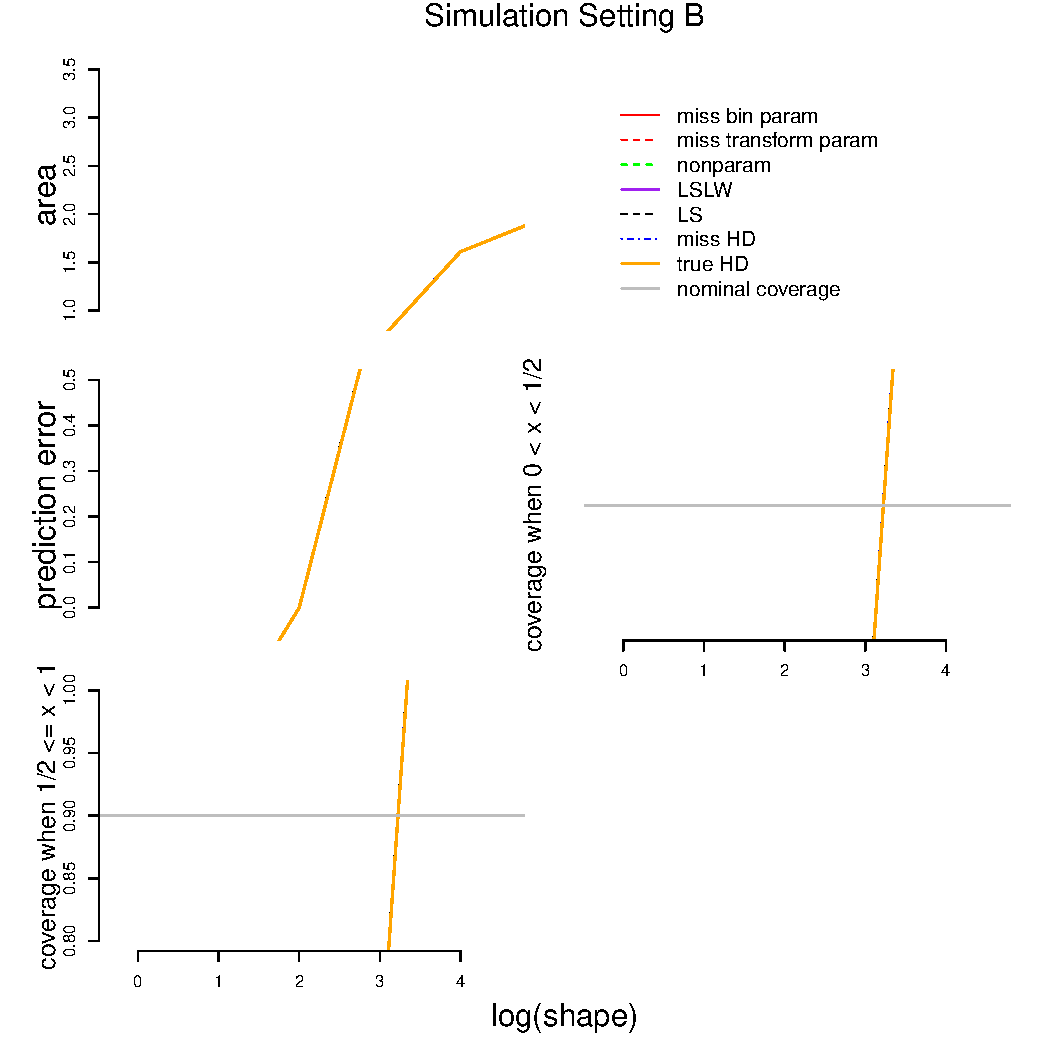
\includegraphics[width=\maxwidth]{figure/Fig-misspec-150-1} 

\end{knitrout}
\end{center}
\caption{This figure compares the performance of the 
  misspecified binned parametric,
  misspecified transformation,  
  binned nonparametric,
  least squares, and 
  least squares locally weighted conformal prediction regions and the 
  misspecified and correctly specified highest density prediction regions 
  when $n = 150$ and the number of bins equals 2.  
  The specific diagnostics used to compare these prediction regions is the 
    area,
    prediction error, 
    marginal coverage probability, 
    and the coverage probability with respect to binning  
    across shape parameter values.
  The average of 200 Monte Carlo samples at each shape parameter value in 
  these simulation settings form the lines that are depicted in this figure.}
\label{Fig:misspec.150}
\end{figure}



% local coverage, n = 150
\newpage
\begin{figure}[h!]
\begin{center}
\begin{knitrout}
\definecolor{shadecolor}{rgb}{0.969, 0.969, 0.969}\color{fgcolor}
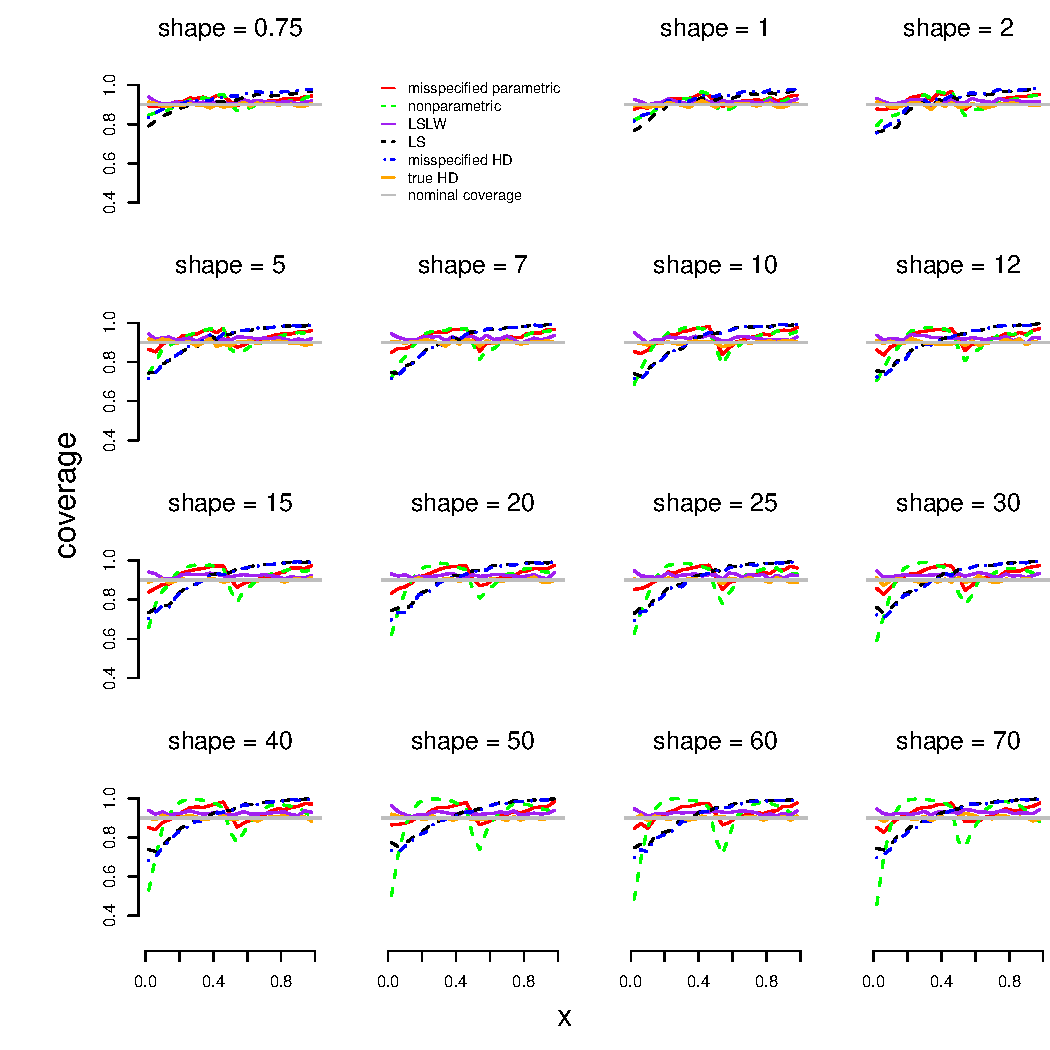
\includegraphics[width=\maxwidth]{figure/Fig-misspec-inx-150-1} 

\end{knitrout}
\end{center}
\caption{Plot of the estimated coverage probabilities of prediction regions 
  across $x$ and shape parameter values when the model is misspecified, 
  $n = 150$, and the number of bins is equal to $2$.}
\label{Fig:misspec.inx.150}
\end{figure}


% Diagnostics, n = 250
\newpage
\begin{figure}[h!]
\begin{center}
\begin{knitrout}
\definecolor{shadecolor}{rgb}{0.969, 0.969, 0.969}\color{fgcolor}
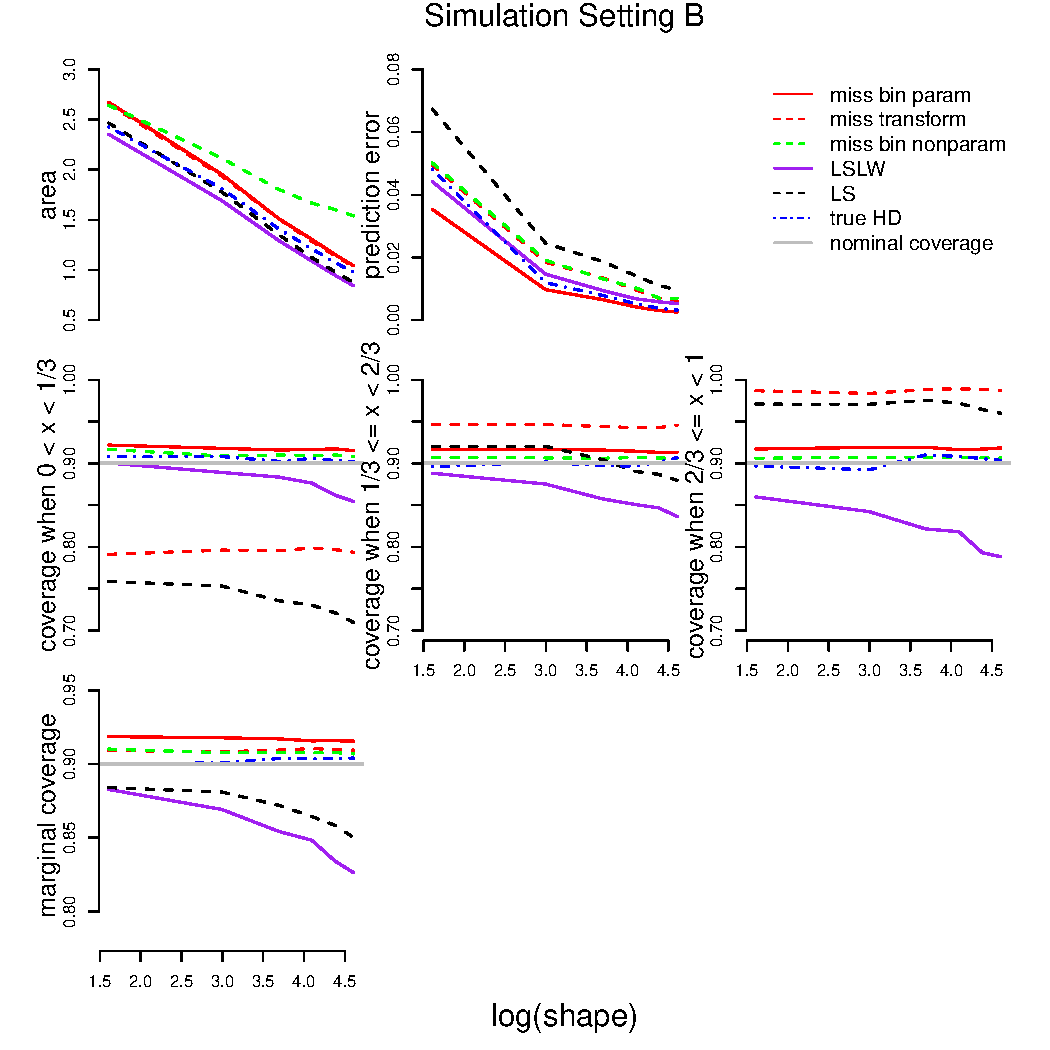
\includegraphics[width=\maxwidth]{figure/Fig-misspec-250-1} 

\end{knitrout}
\end{center}
\caption{This figure compares the performance of the 
  misspecified binned parametric,
  misspecified transformation, 
  binned nonparametric,
  least squares, and 
  least squares locally weighted conformal prediction region and the 
  correctly specified highest density prediction regions when $n = 250$ 
  and the number of bins equals 3.  
  The specific diagnostics used to compare these prediction regions is the 
    area,
    prediction error, 
    marginal coverage probability,     
    and the coverage probability with respect to binning 
    across shape parameter values.
  The average of 50 Monte Carlo samples at each shape parameter value in 
  these simulation settings form the lines that are depicted in this figure.}
\label{Fig:misspec.250}
\end{figure}



% local coverage, n = 250
\newpage
\begin{figure}[h!]
\begin{center}
\begin{knitrout}
\definecolor{shadecolor}{rgb}{0.969, 0.969, 0.969}\color{fgcolor}
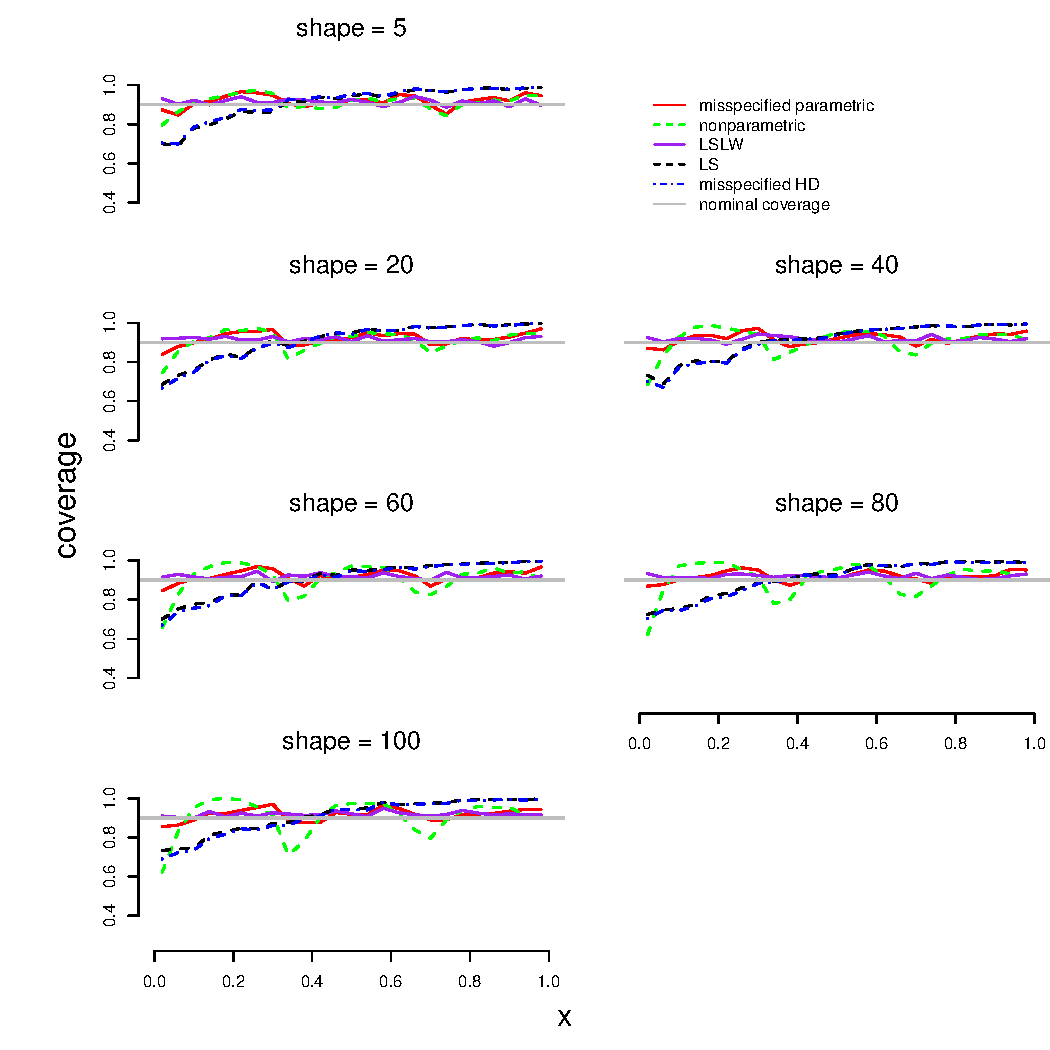
\includegraphics[width=\maxwidth]{figure/Fig-misspec-inx-250-1} 

\end{knitrout}
\end{center}
\caption{Plot of the estimated coverage probabilities of prediction regions 
  across $x$ and shape parameter values when the model is misspecified, 
  $n = 250$, and the number of bins is equal to $3$.}
\label{Fig:misspec.inx.250}
\end{figure}



% Diagnostics, n = 500
\newpage
\begin{figure}[h!]
\begin{center}
\begin{knitrout}
\definecolor{shadecolor}{rgb}{0.969, 0.969, 0.969}\color{fgcolor}
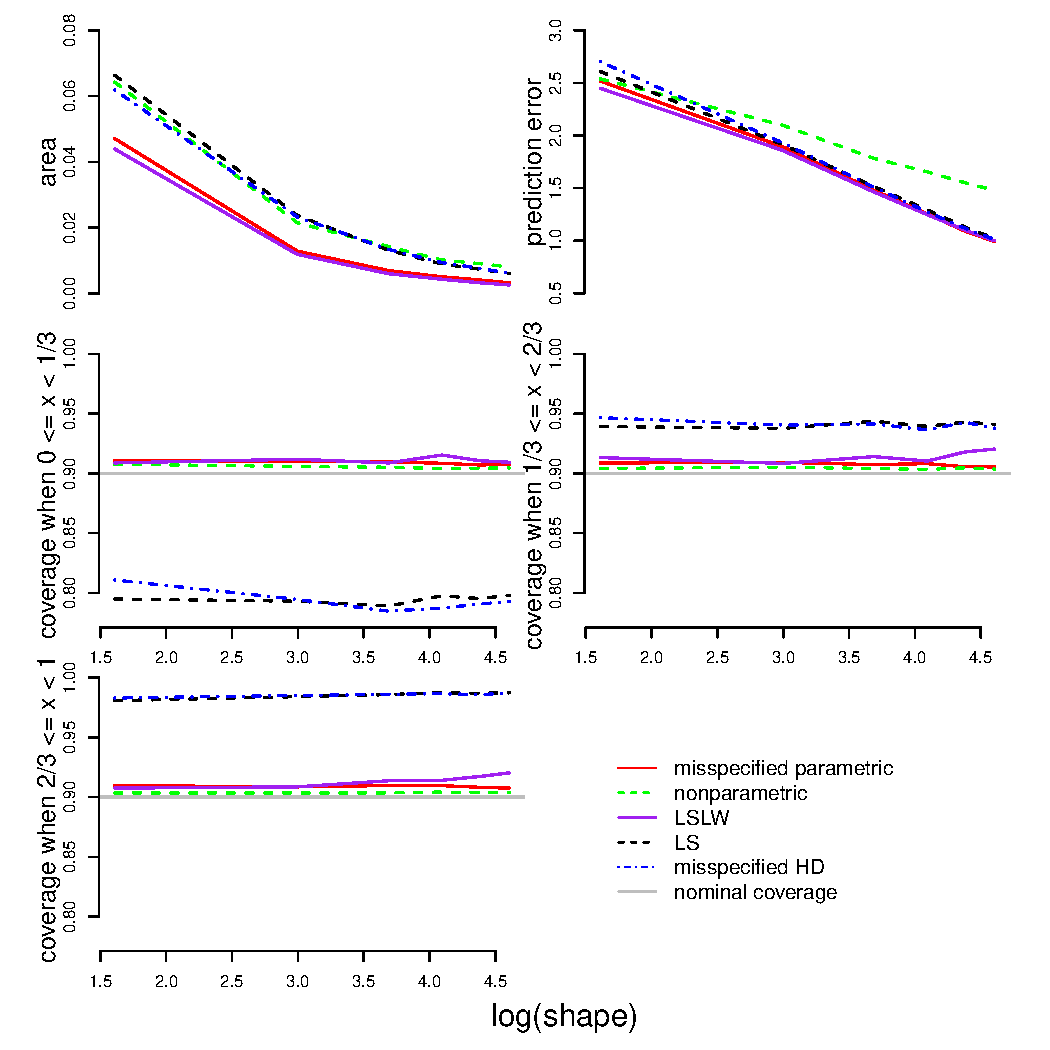
\includegraphics[width=\maxwidth]{figure/Fig-misspec-500-1} 

\end{knitrout}
\end{center}
\caption{This figure compares the performance of the 
  binned misspecified parametric, 
  misspecified transformation, 
  binned nonparametric,
  least squares, and 
  least squares locally weighted conformal prediction regions and the 
  correctly specified highest density prediction region when $n = 500$ and the 
  number of bins equals 3.  
  The specific diagnostics used to compare these prediction regions is the 
    area,
    prediction error, 
    marginal coverage probability,     
    and the coverage probability with respect to binning  
    across shape parameter values.
  The average of 50 Monte Carlo samples at each shape parameter value in 
  these simulation settings form the lines that are depicted in this figure.}
\label{Fig:misspec.500}
\end{figure}



% local coverage, n = 500
\newpage
\begin{figure}[h!]
\begin{center}
\begin{knitrout}
\definecolor{shadecolor}{rgb}{0.969, 0.969, 0.969}\color{fgcolor}
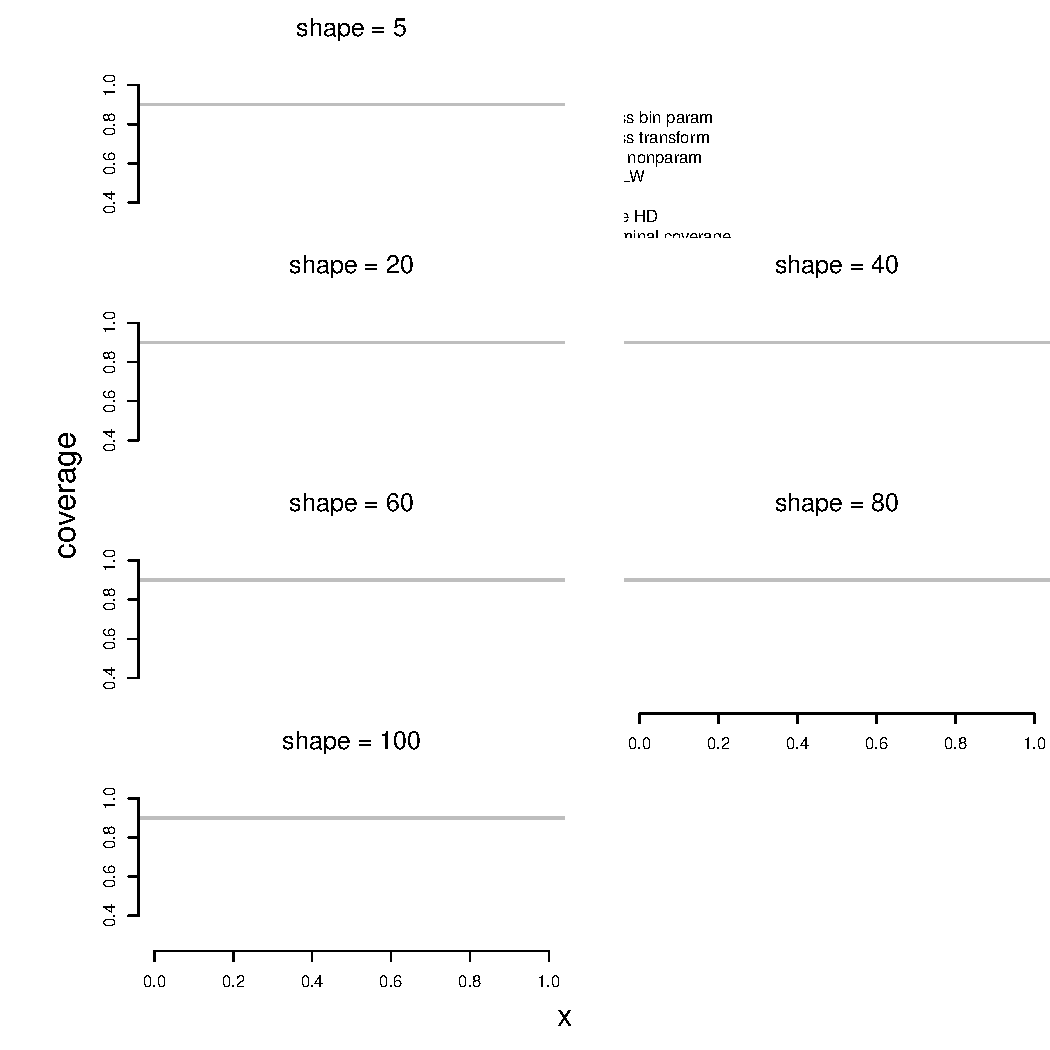
\includegraphics[width=\maxwidth]{figure/Fig-misspec-inx-500-1} 

\end{knitrout}
\end{center}
\caption{Plot of the estimated coverage probabilities of prediction regions 
  across $x$ and shape parameter values when the model is misspecified, 
  $n = 500$, and the number of bins is equal to $3$.}
\label{Fig:misspec.inx.500}
\end{figure}





\newpage
\section{Linear Regression Simulations}
\label{sec:regression}

In this Section, we compare both parametric conformal prediction 
regions, the binned nonparametric conformal prediction region, the LSLW conformal 
prediction region, the LS conformal prediction region, and the HD prediction 
region for linear regression models with normal errors and constant variance.  
We specify that $\beta = (2, 5)^T$ and the standard deviation of the errors 
about the mean function as $\sigma = 1$.
We consider sample sizes of $n \in \{150, 250, 500\}$. 
When $n = 150$ we build the binned parametric and nonparametric conformal 
prediction regions using 2 bins.  When $n = 250, 500$ we build the parametric 
and nonparametric conformal prediction regions using 3 bins.  These number of 
bin choices correspond to the bin width asymptotics of 
\citet{lei2014distribution}. 


\subsection{Simulations}

The following function computes our diagnostic measures for the five 
prediction regions under investigation in the univariate case where data 
is generated from a Gaussian regression model, i.e. 
$Y \sim N(X'\beta, \sigma^2)$ and $X \sim U(0,1)$.

\begin{knitrout}
\definecolor{shadecolor}{rgb}{0.969, 0.969, 0.969}\color{fgcolor}\begin{kframe}
\begin{alltt}
\hlstd{regression_simulator} \hlkwb{<-} \hlkwa{function}\hlstd{(}\hlkwc{beta}\hlstd{,} \hlkwc{n} \hlstd{=} \hlnum{150}\hlstd{,} \hlkwc{sd} \hlstd{=} \hlnum{1}\hlstd{,}
  \hlkwc{alpha} \hlstd{=} \hlnum{0.10}\hlstd{,} \hlkwc{B} \hlstd{=} \hlnum{2}\hlstd{,} \hlkwc{bins} \hlstd{= bins)\{}

  \hlstd{p} \hlkwb{<-} \hlstd{d} \hlkwb{<-} \hlkwd{length}\hlstd{(beta)} \hlopt{-} \hlnum{1}

  \hlstd{models} \hlkwb{<-} \hlkwd{lapply}\hlstd{(}\hlnum{1}\hlopt{:}\hlstd{B,} \hlkwc{FUN} \hlstd{=} \hlkwa{function}\hlstd{(}\hlkwc{j}\hlstd{)\{}
    \hlstd{x} \hlkwb{<-} \hlkwd{matrix}\hlstd{(}\hlkwd{runif}\hlstd{(n),} \hlkwc{ncol} \hlstd{= p)}
    \hlstd{mu} \hlkwb{<-} \hlkwd{cbind}\hlstd{(}\hlnum{1}\hlstd{, x)} \hlopt \hlstd{beta}
    \hlstd{y} \hlkwb{<-} \hlkwd{rnorm}\hlstd{(}\hlkwc{n} \hlstd{= n,} \hlkwc{mean} \hlstd{= mu,} \hlkwc{sd} \hlstd{= sd)}
    \hlstd{y} \hlkwb{<-} \hlstd{y} \hlopt{/} \hlkwd{sd}\hlstd{(y)}
    \hlstd{dat} \hlkwb{<-} \hlkwd{data.frame}\hlstd{(}\hlkwc{y} \hlstd{= y,} \hlkwc{x} \hlstd{= x)}
    \hlkwd{colnames}\hlstd{(dat)[}\hlnum{2}\hlopt{:}\hlstd{(p}\hlopt{+}\hlnum{1}\hlstd{)]} \hlkwb{<-} \hlkwd{paste}\hlstd{(}\hlstr{"x"}\hlstd{,} \hlnum{1}\hlopt{:}\hlstd{p,} \hlkwc{sep} \hlstd{=} \hlstr{""}\hlstd{)}
    \hlstd{fit} \hlkwb{<-} \hlkwd{glm}\hlstd{(y} \hlopt{~} \hlstd{x1,} \hlkwc{family} \hlstd{=} \hlstr{"gaussian"}\hlstd{,}
      \hlkwc{data} \hlstd{= dat,} \hlkwc{x} \hlstd{=} \hlnum{TRUE}\hlstd{,} \hlkwc{y} \hlstd{=} \hlnum{TRUE}\hlstd{)}
    \hlstd{output} \hlkwb{=} \hlkwd{list}\hlstd{(}\hlkwc{model} \hlstd{= fit,} \hlkwc{dat} \hlstd{= dat)}
    \hlstd{output}
  \hlstd{\})}

  \hlstd{funs} \hlkwb{<-} \hlkwd{lm.funs}\hlstd{(}\hlkwc{intercept} \hlstd{=} \hlnum{TRUE}\hlstd{)}
  \hlstd{train.fun} \hlkwb{<-} \hlstd{funs}\hlopt{$}\hlstd{train.fun}
  \hlstd{predict.fun} \hlkwb{<-} \hlstd{funs}\hlopt{$}\hlstd{predict.fun}
  \hlstd{conformal_regions} \hlkwb{<-} \hlkwd{lapply}\hlstd{(models,} \hlkwc{FUN} \hlstd{=} \hlkwa{function}\hlstd{(}\hlkwc{obj}\hlstd{)\{}

    \hlstd{model} \hlkwb{<-} \hlstd{obj}\hlopt{$}\hlstd{model}
    \hlstd{dat} \hlkwb{<-} \hlstd{obj}\hlopt{$}\hlstd{dat}
    \hlstd{model}\hlopt{$}\hlstd{data} \hlkwb{<-} \hlstd{dat}
    \hlstd{x} \hlkwb{<-} \hlstd{model}\hlopt{$}\hlstd{x[,} \hlnum{2}\hlstd{]}
    \hlstd{y} \hlkwb{<-} \hlstd{model}\hlopt{$}\hlstd{y}

    \hlstd{fit.int} \hlkwb{<-} \hlkwd{lm}\hlstd{(y} \hlopt{~} \hlstd{x,} \hlkwc{data} \hlstd{= dat)}
    \hlstd{betaMLE} \hlkwb{<-} \hlkwd{coefficients}\hlstd{(fit.int)}
    \hlstd{sdMLE} \hlkwb{<-} \hlkwd{summary}\hlstd{(fit.int)}\hlopt{$}\hlstd{sigma}
    \hlstd{meanMLE} \hlkwb{<-} \hlkwd{as.numeric}\hlstd{(}\hlkwd{cbind}\hlstd{(}\hlnum{1}\hlstd{, x)} \hlopt \hlstd{betaMLE)}
    \hlstd{HDCI} \hlkwb{<-} \hlkwd{do.call}\hlstd{(rbind,} \hlkwd{lapply}\hlstd{(}\hlnum{1}\hlopt{:}\hlstd{n,} \hlkwa{function}\hlstd{(}\hlkwc{j}\hlstd{)\{}
      \hlkwd{hdi}\hlstd{(qnorm,} \hlnum{1} \hlopt{-} \hlstd{alpha,} \hlkwc{mean} \hlstd{= meanMLE[j],} \hlkwc{sd} \hlstd{= sdMLE)}
    \hlstd{\}))}

    \hlstd{p1.tibs} \hlkwb{<-} \hlkwd{conformal.pred}\hlstd{(}\hlkwc{x} \hlstd{= x,} \hlkwc{y} \hlstd{= y,} \hlkwc{x0} \hlstd{= x,}
      \hlkwc{train.fun} \hlstd{= train.fun,} \hlkwc{predict.fun} \hlstd{= predict.fun,}
      \hlkwc{alpha} \hlstd{= alpha)}
    \hlstd{LSCI} \hlkwb{<-} \hlkwd{cbind}\hlstd{(p1.tibs}\hlopt{$}\hlstd{lo, p1.tibs}\hlopt{$}\hlstd{up)}

    \hlstd{abs.resid} \hlkwb{<-} \hlkwd{abs}\hlstd{(fit.int}\hlopt{$}\hlstd{resid)}
    \hlstd{smooth.call} \hlkwb{<-} \hlkwd{smooth.spline}\hlstd{(x, abs.resid,}
      \hlkwc{nknots} \hlstd{=} \hlnum{10}\hlstd{)}
    \hlstd{lambda} \hlkwb{<-} \hlstd{smooth.call}\hlopt{$}\hlstd{lambda}
    \hlstd{df} \hlkwb{<-} \hlstd{smooth.call}\hlopt{$}\hlstd{df}
    \hlstd{mad.train.fun} \hlkwb{<-} \hlkwa{function}\hlstd{(}\hlkwc{x}\hlstd{,} \hlkwc{y}\hlstd{,} \hlkwc{out} \hlstd{=} \hlkwa{NULL}\hlstd{)\{}
      \hlkwd{smooth.spline}\hlstd{(x[,} \hlnum{1}\hlstd{], y,} \hlkwc{lambda} \hlstd{= lambda,}
      \hlkwc{df} \hlstd{= df,} \hlkwc{nknots} \hlstd{=} \hlnum{10}\hlstd{)}
    \hlstd{\}}
    \hlstd{mad.predict.fun} \hlkwb{<-} \hlkwa{function}\hlstd{(}\hlkwc{out}\hlstd{,} \hlkwc{newx}\hlstd{)\{}
      \hlkwd{predict}\hlstd{(out,} \hlkwd{as.data.frame}\hlstd{(newx))}\hlopt{$}\hlstd{y[,} \hlnum{1}\hlstd{]}
    \hlstd{\}}
    \hlstd{p2.tibs} \hlkwb{<-} \hlkwd{conformal.pred}\hlstd{(}\hlkwc{x} \hlstd{= x,} \hlkwc{y} \hlstd{= y,} \hlkwc{x0} \hlstd{= x,}
      \hlkwc{train.fun} \hlstd{= train.fun,} \hlkwc{predict.fun} \hlstd{= predict.fun,}
      \hlkwc{mad.train.fun} \hlstd{= mad.train.fun,}
      \hlkwc{mad.predict.fun} \hlstd{= mad.predict.fun,}
      \hlkwc{alpha} \hlstd{= alpha)}
    \hlstd{LSLWCI} \hlkwb{<-} \hlkwd{cbind}\hlstd{(p2.tibs}\hlopt{$}\hlstd{lo, p2.tibs}\hlopt{$}\hlstd{up)}

    \hlstd{conf} \hlkwb{<-} \hlkwd{conformal.glm}\hlstd{(model,} \hlkwc{nonparametric} \hlstd{=} \hlnum{TRUE}\hlstd{,} \hlkwc{method} \hlstd{=} \hlstr{"both"}\hlstd{,}
      \hlkwc{bins} \hlstd{= bins,} \hlkwc{cores} \hlstd{=} \hlnum{7}\hlstd{)}
    \hlstd{parabinCI} \hlkwb{<-} \hlstd{conf}\hlopt{$}\hlstd{paraconfbin}
    \hlstd{transformCI} \hlkwb{<-} \hlstd{conf}\hlopt{$}\hlstd{transformconf}
    \hlstd{nonparabinCI} \hlkwb{<-} \hlstd{conf}\hlopt{$}\hlstd{nonparaconfbin}

    \hlstd{out} \hlkwb{=} \hlkwd{list}\hlstd{(}\hlkwc{parabinCI} \hlstd{= parabinCI,} \hlkwc{transformCI} \hlstd{= transformCI,}
      \hlkwc{nonparabinCI} \hlstd{= nonparabinCI,} \hlkwc{LSLWCI} \hlstd{= LSLWCI,} \hlkwc{LSCI} \hlstd{= LSCI,}
      \hlkwc{HDCI} \hlstd{= HDCI)}
    \hlstd{out}
  \hlstd{\})}


  \hlstd{diagnostics_regions} \hlkwb{<-} \hlkwd{lapply}\hlstd{(}\hlnum{1}\hlopt{:}\hlstd{B,} \hlkwc{FUN} \hlstd{=} \hlkwa{function}\hlstd{(}\hlkwc{j}\hlstd{)\{}

    \hlstd{obj} \hlkwb{<-} \hlstd{conformal_regions[[j]]}
    \hlstd{dat} \hlkwb{<-} \hlkwd{as.data.frame}\hlstd{(models[[j]]}\hlopt{$}\hlstd{dat)}
    \hlstd{y} \hlkwb{<-} \hlkwd{as.numeric}\hlstd{(dat[,} \hlnum{1}\hlstd{])}

    \hlstd{diagnostics} \hlkwb{<-} \hlkwd{lapply}\hlstd{(obj,} \hlkwc{FUN} \hlstd{=} \hlkwa{function}\hlstd{(}\hlkwc{region}\hlstd{)\{}

      \hlstd{output} \hlkwb{<-} \hlkwa{NULL}
      \hlkwa{if}\hlstd{(}\hlkwd{class}\hlstd{(region)} \hlopt{==} \hlstr{"matrix"}\hlstd{)\{}
        \hlstd{marginal.coverage} \hlkwb{<-} \hlkwd{local.coverage}\hlstd{(}\hlkwc{region} \hlstd{= region,}
          \hlkwc{data} \hlstd{= dat,} \hlkwc{d} \hlstd{= p,} \hlkwc{bins} \hlstd{=} \hlnum{1}\hlstd{,} \hlkwc{at.data} \hlstd{=} \hlstr{"TRUE"}\hlstd{)}
        \hlstd{local.coverage} \hlkwb{<-} \hlkwd{local.coverage}\hlstd{(}\hlkwc{region} \hlstd{= region,}
          \hlkwc{data} \hlstd{= dat,} \hlkwc{d} \hlstd{= p,} \hlkwc{bins} \hlstd{= bins,} \hlkwc{at.data} \hlstd{=} \hlstr{"TRUE"}\hlstd{)}
        \hlstd{local.inx.coverage} \hlkwb{<-} \hlkwd{local.coverage}\hlstd{(}\hlkwc{region} \hlstd{= region,}
          \hlkwc{data} \hlstd{= dat,} \hlkwc{d} \hlstd{= p,} \hlkwc{bins} \hlstd{=} \hlnum{25}\hlstd{,} \hlkwc{at.data} \hlstd{=} \hlstr{"TRUE"}\hlstd{)}
        \hlstd{output} \hlkwb{<-} \hlkwd{c}\hlstd{(marginal.coverage, local.coverage,}
          \hlstd{local.inx.coverage,} \hlkwd{mean}\hlstd{(}\hlkwd{apply}\hlstd{(region,} \hlnum{1}\hlstd{, diff)),}
          \hlkwd{absolute.error}\hlstd{(}\hlkwc{y} \hlstd{= y,} \hlkwc{region} \hlstd{= region))}
      \hlstd{\}}
      \hlkwa{else}\hlstd{\{}
        \hlstd{marginal.coverage} \hlkwb{<-} \hlkwd{local.coverage}\hlstd{(}\hlkwc{region} \hlstd{= region,}
          \hlkwc{nonparametric} \hlstd{=} \hlstr{"TRUE"}\hlstd{,} \hlkwc{data} \hlstd{= dat,} \hlkwc{d} \hlstd{= p,} \hlkwc{bins} \hlstd{=} \hlnum{1}\hlstd{,}
          \hlkwc{at.data} \hlstd{=} \hlstr{"TRUE"}\hlstd{)}
        \hlstd{local.coverage} \hlkwb{<-} \hlkwd{local.coverage}\hlstd{(}\hlkwc{region} \hlstd{= region,}
          \hlkwc{nonparametric} \hlstd{=} \hlstr{"TRUE"}\hlstd{,} \hlkwc{data} \hlstd{= dat,} \hlkwc{d} \hlstd{= p,} \hlkwc{bins} \hlstd{= bins,}
          \hlkwc{at.data} \hlstd{=} \hlstr{"TRUE"}\hlstd{)}
        \hlstd{local.inx.coverage} \hlkwb{<-} \hlkwd{local.coverage}\hlstd{(}\hlkwc{region} \hlstd{= region,}
          \hlkwc{nonparametric} \hlstd{=} \hlstr{"TRUE"}\hlstd{,} \hlkwc{data} \hlstd{= dat,} \hlkwc{d} \hlstd{= p,} \hlkwc{bins} \hlstd{=} \hlnum{25}\hlstd{,}
          \hlkwc{at.data} \hlstd{=} \hlstr{"TRUE"}\hlstd{)}
        \hlstd{output} \hlkwb{<-} \hlkwd{c}\hlstd{(marginal.coverage, local.coverage,}
          \hlstd{local.inx.coverage,} \hlkwd{area.nonparametric}\hlstd{(region),}
          \hlkwd{absolute.error.nonparametric}\hlstd{(}\hlkwc{data} \hlstd{= dat,}
            \hlkwc{region} \hlstd{= region))}
      \hlstd{\}}
      \hlstd{output}
    \hlstd{\})}
    \hlkwd{do.call}\hlstd{(rbind, diagnostics)}

  \hlstd{\})}

  \hlstd{diagnostics_regions}
\hlstd{\}}
\end{alltt}
\end{kframe}
\end{knitrout}



The following performs our Monte Carlo simulation of $B = 50$ iterations 
when $n = 150$.


\begin{knitrout}
\definecolor{shadecolor}{rgb}{0.969, 0.969, 0.969}\color{fgcolor}\begin{kframe}
\begin{alltt}
\hlkwd{set.seed}\hlstd{(}\hlnum{13}\hlstd{)}
\hlstd{beta} \hlkwb{<-} \hlkwd{c}\hlstd{(}\hlnum{2}\hlstd{,} \hlnum{5}\hlstd{)}
\hlstd{n} \hlkwb{<-} \hlnum{150}
\hlstd{bins} \hlkwb{<-} \hlnum{2}
\hlstd{B} \hlkwb{<-} \hlnum{50}
\hlkwd{set.seed}\hlstd{(}\hlnum{13}\hlstd{)}
\hlkwd{system.time}\hlstd{(out.regression.150} \hlkwb{<-} \hlkwd{do.call}\hlstd{(rbind,}
  \hlkwd{regression_simulator}\hlstd{(}\hlkwc{beta} \hlstd{= beta,} \hlkwc{n} \hlstd{= n,} \hlkwc{bins} \hlstd{= bins,} \hlkwc{B} \hlstd{= B)))}
\end{alltt}
\begin{verbatim}
##     user   system  elapsed 
## 3001.006   41.021 1406.746
\end{verbatim}
\begin{alltt}
\hlstd{diagnostics.regression.150} \hlkwb{<-} \hlkwd{do.call}\hlstd{(rbind,} \hlkwd{lapply}\hlstd{(}\hlkwd{split}\hlstd{(out.regression.150,}
  \hlkwc{f} \hlstd{=} \hlkwd{as.factor}\hlstd{(}\hlkwd{rownames}\hlstd{(out.regression.150))),}
  \hlkwc{FUN} \hlstd{=} \hlkwa{function}\hlstd{(}\hlkwc{xx}\hlstd{)} \hlkwd{colMeans}\hlstd{(}\hlkwd{matrix}\hlstd{(xx,} \hlkwc{nrow} \hlstd{= B),} \hlkwc{na.rm} \hlstd{=} \hlnum{TRUE}\hlstd{)))}
\end{alltt}
\end{kframe}
\end{knitrout}


The following performs our Monte Carlo simulation of $B = 50$ iterations 
when $n = 250$.

\begin{knitrout}
\definecolor{shadecolor}{rgb}{0.969, 0.969, 0.969}\color{fgcolor}\begin{kframe}
\begin{alltt}
\hlkwd{set.seed}\hlstd{(}\hlnum{13}\hlstd{)}
\hlstd{beta} \hlkwb{<-} \hlkwd{c}\hlstd{(}\hlnum{2}\hlstd{,} \hlnum{5}\hlstd{)}
\hlstd{n} \hlkwb{<-} \hlnum{250}
\hlstd{bins} \hlkwb{<-} \hlnum{3}
\hlstd{B} \hlkwb{<-} \hlnum{50}
\hlkwd{set.seed}\hlstd{(}\hlnum{13}\hlstd{)}
\hlkwd{system.time}\hlstd{(out.regression.250} \hlkwb{<-} \hlkwd{do.call}\hlstd{(rbind,}
  \hlkwd{regression_simulator}\hlstd{(}\hlkwc{beta} \hlstd{= beta,} \hlkwc{n} \hlstd{= n,} \hlkwc{bins} \hlstd{= bins,} \hlkwc{B} \hlstd{= B)))}
\end{alltt}
\begin{verbatim}
##     user   system  elapsed 
## 5047.225   42.288 2400.109
\end{verbatim}
\begin{alltt}
\hlstd{diagnostics.regression.250} \hlkwb{<-} \hlkwd{do.call}\hlstd{(rbind,} \hlkwd{lapply}\hlstd{(}\hlkwd{split}\hlstd{(out.regression.250,}
  \hlkwc{f} \hlstd{=} \hlkwd{as.factor}\hlstd{(}\hlkwd{rownames}\hlstd{(out.regression.150))),}
  \hlkwc{FUN} \hlstd{=} \hlkwa{function}\hlstd{(}\hlkwc{xx}\hlstd{)} \hlkwd{colMeans}\hlstd{(}\hlkwd{matrix}\hlstd{(xx,} \hlkwc{nrow} \hlstd{= B),} \hlkwc{na.rm} \hlstd{=} \hlnum{TRUE}\hlstd{)))}
\end{alltt}
\end{kframe}
\end{knitrout}


The following performs our Monte Carlo simulation of $B = 50$ iterations 
when $n = 500$.

\begin{knitrout}
\definecolor{shadecolor}{rgb}{0.969, 0.969, 0.969}\color{fgcolor}\begin{kframe}
\begin{alltt}
\hlkwd{set.seed}\hlstd{(}\hlnum{13}\hlstd{)}
\hlstd{beta} \hlkwb{<-} \hlkwd{c}\hlstd{(}\hlnum{2}\hlstd{,} \hlnum{5}\hlstd{)}
\hlstd{n} \hlkwb{<-} \hlnum{500}
\hlstd{bins} \hlkwb{<-} \hlnum{3}
\hlstd{B} \hlkwb{<-} \hlnum{50}
\hlkwd{set.seed}\hlstd{(}\hlnum{13}\hlstd{)}
\hlkwd{system.time}\hlstd{(out.regression.500} \hlkwb{<-} \hlkwd{do.call}\hlstd{(rbind,}
  \hlkwd{regression_simulator}\hlstd{(}\hlkwc{beta} \hlstd{= beta,} \hlkwc{n} \hlstd{= n,} \hlkwc{bins} \hlstd{= bins,} \hlkwc{B} \hlstd{= B)))}
\end{alltt}
\begin{verbatim}
##     user   system  elapsed 
## 12687.89    55.73  6168.26
\end{verbatim}
\begin{alltt}
\hlstd{diagnostics.regression.500} \hlkwb{<-} \hlkwd{do.call}\hlstd{(rbind,} \hlkwd{lapply}\hlstd{(}\hlkwd{split}\hlstd{(out.regression.500,}
  \hlkwc{f} \hlstd{=} \hlkwd{as.factor}\hlstd{(}\hlkwd{rownames}\hlstd{(out.regression.150))),}
  \hlkwc{FUN} \hlstd{=} \hlkwa{function}\hlstd{(}\hlkwc{xx}\hlstd{)} \hlkwd{colMeans}\hlstd{(}\hlkwd{matrix}\hlstd{(xx,} \hlkwc{nrow} \hlstd{= B),} \hlkwc{na.rm} \hlstd{=} \hlnum{TRUE}\hlstd{)))}
\end{alltt}
\end{kframe}
\end{knitrout}


\subsection{Results}

Results form our simulations are depicted in 
Table~\ref{Tab:regression-results} and Figure~\ref{Fig:regresion.inx}.  
This table and figure depicts the estimatated area, prediction 
error, and local coverage probabilities for all five considered prediction 
regions. 

In these simulations, errors about the estimated mean function are symmetric 
and homogeneous across the support.  We therefore expect for the LS and LSLW 
conformal prediction regions to perform nearly as well as the oracle HD 
prediction region.  These prediction regions also exhibit finite-sample 
marginal validity, local validity with respect to binning, and near 
conditional validity across the support.  The parametric conformal prediction 
region is similar to the LS and LSLW conformal prediction regions and the HD 
prediction region in area, prediction error, finite-sample coverage 
properties, and appearance.  However, the parametric conformal prediction 
region is slightly larger and gives more conservative coverage that these 
other prediction regions.  The nonparametric conformal prediction region 
is larger and gives larger prediction errors than the other prediction 
regions.  It also appears to not visually fit the data well while the others 
do as seen in Section~\ref{sec:regressionplots}.





\begin{table}[h!]
\scriptsize
\begin{center}
\begin{tabular}{llcccccc}
  & & OLS trans & OLS bin   & bin nonparametric & LS        & LSLW      & HD     \\
  & & conformal & conformal & conformal         & conformal & conformal & region \\ 
  $n = 150$
    & marginal coverage &
  $0.911$ & 
  $0.919$ & 
  $0.911$ & 
  $0.878$ & 
  $0.883$ & 
  $0.904$ \\
    & local coverage when $0 < x < 1/2$ & 
  $0.912$ & 
  $0.918$ & 
  $0.911$ & 
  $0.878$ & 
  $0.886$ & 
  $0.903$ \\
    & local coverage when $1/2 \leq x < 1$ & 
  $0.909$ & 
  $0.92$ & 
  $0.911$ & 
  $0.878$ & 
  $0.881$ & 
  $0.904$ \\
    & area &
  $1.88$ & 
  $1.994$ & 
  $2.408$ & 
  $1.775$ & 
  $1.782$ & 
  $1.872$ \\
    & prediction error &
  $0.01$ & 
  $0.007$ & 
  $0.011$ & 
  $0.012$ & 
  $0.011$ & 
  $0.01$ \\
  \hline
  $n = 250$  
    & marginal coverage &
  $0.908$ & 
  $0.916$ & 
  $0.909$ & 
  $0.875$ & 
  $0.878$ & 
  $0.902$ \\
    & local coverage when $0 < x < 1/3$ & 
  $0.9$ & 
  $0.916$ & 
  $0.909$ & 
  $0.87$ & 
  $0.882$ & 
  $0.896$ \\
    & local coverage when $1/3 \leq x < 2/3$ & 
  $0.914$ & 
  $0.913$ & 
  $0.909$ & 
  $0.879$ & 
  $0.876$ & 
  $0.907$ \\
    & local coverage when $2/3 \leq x < 1$ &
  $0.909$ & 
  $0.92$ & 
  $0.909$ & 
  $0.877$ & 
  $0.876$ & 
  $0.904$ \\
    & area & 
  $1.877$ & 
  $1.974$ & 
  $2.139$ & 
  $1.751$ & 
  $1.754$ & 
  $1.864$ \\
    & prediction error & 
  $0.009$ & 
  $0.007$ & 
  $0.01$ & 
  $0.013$ & 
  $0.012$ & 
  $0.01$ \\
  \hline
  $n = 500$
    & marginal coverage &
  $0.908$ & 
  $0.907$ & 
  $0.904$ & 
  $0.875$ & 
  $0.873$ & 
  $0.902$ \\
    & local coverage when $0 < x < 1/3$ & 
  $0.911$ & 
  $0.908$ & 
  $0.906$ & 
  $0.878$ & 
  $0.875$ & 
  $0.905$ \\
    & local coverage when $1/3 \leq x < 2/3$ & 
  $0.907$ & 
  $0.907$ & 
  $0.904$ & 
  $0.874$ & 
  $0.871$ & 
  $0.902$ \\
    & local coverage when $2/3 \leq x < 1$ &
  $0.905$ & 
  $0.907$ & 
  $0.904$ & 
  $0.874$ & 
  $0.875$ & 
  $0.899$ \\
    & area & 
  $1.886$ & 
  $1.904$ & 
  $2.098$ & 
  $1.735$ & 
  $1.731$ & 
  $1.86$ \\
    & prediction error & 
  $0.009$ & 
  $0.009$ & 
  $0.011$ & 
  $0.013$ & 
  $0.013$ & 
  $0.01$ 
\end{tabular}
\end{center}
\caption{Diagnostics for conformal prediction regions for linear regression 
  models with normal errors and constant variance.  Local and marginal 
  coverage properties, areas, and prediction errors are presented for the 
    transformation based and binned parametric conformal prediction regions,
    binned nonparametric conformal prediction region,
    LS conformal prediction region, 
    LSLW conformal prediction region, and 
    HD prediction region.} %Standard errors are in parentheses.}
\label{Tab:regression-results}
\end{table}







\newpage
\begin{figure}[h!]
\begin{center}
\begin{knitrout}
\definecolor{shadecolor}{rgb}{0.969, 0.969, 0.969}\color{fgcolor}
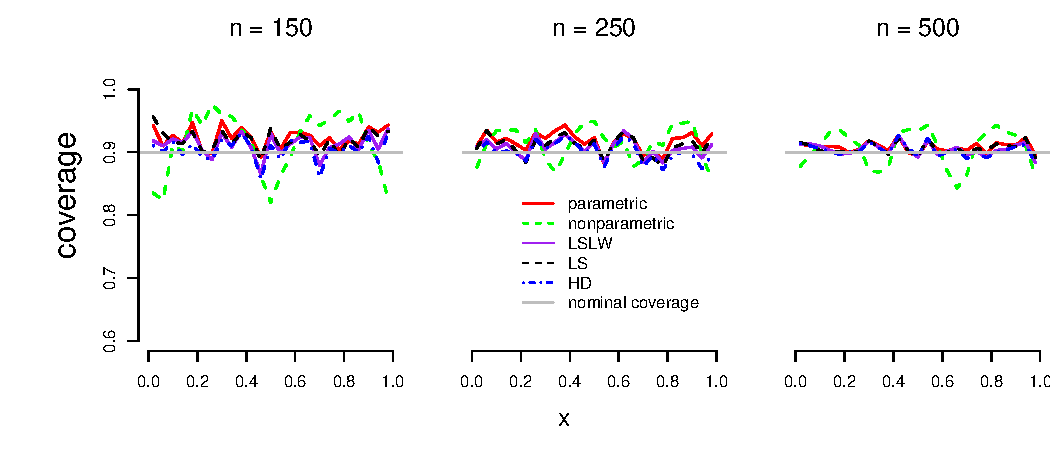
\includegraphics[width=\maxwidth]{figure/Fig-regression-inx-500-1} 

\end{knitrout}
\end{center}
\caption{Plot of the estimated coverage probabilities of prediction regions 
  across $x$ and sample sizes.}
\label{Fig:regresion.inx}
\end{figure}




\newpage
\section{Example plots of prediction regions}
\label{sec:plotsofregions}

In this section we construct prediction regions corresponding to the 
simulations and results in Sections~\ref{sec:Gamma} through 
\ref{sec:regressionplots}.  In Gamma analyses we generate a dataset for each 
shape parameter considered with $n = 150$ and in regression analyses we 
generate a dataset for all sample sizes considered.  For each of these datasets 
we depict the parametric, nonparametric, LS, LSLW conformal prediction regions 
over the observed data to visually assess the appropriateness of each 
prediction region.  The findings from these figures are consistent with the 
findings from our numerical diagnostics.  
The parametric conformal prediction region gives visually natural bounds for 
the observed data when the model is correctly specified in small to moderate 
sample sizes and is appropriate when the model is misspecified. 
The LSLW conformal prediction region gives visually natural bounds for the 
observed data when the model is correctly specified, is appropriate under mild 
model misspecification, and is ill-fitting in settings where deviations about 
an estimated mean function are clearly not symmetric.
The nonparametric conformal prediction region is coarse and is larger than 
necessary when the mean function is steep relative to its variability.  
The LS conformal prediction performs well when deviations about the estimated 
mean function are symmetirc and is sensitive to mild departures from that 
setting.  This prediction region is seen to provide overcoverage 
(undercoverage) in regions of the predictor space where variability about the 
estimated mean function is relatively small (large).



\newpage
\begin{figure}[h!]
\begin{center}
\begin{knitrout}
\definecolor{shadecolor}{rgb}{0.969, 0.969, 0.969}\color{fgcolor}
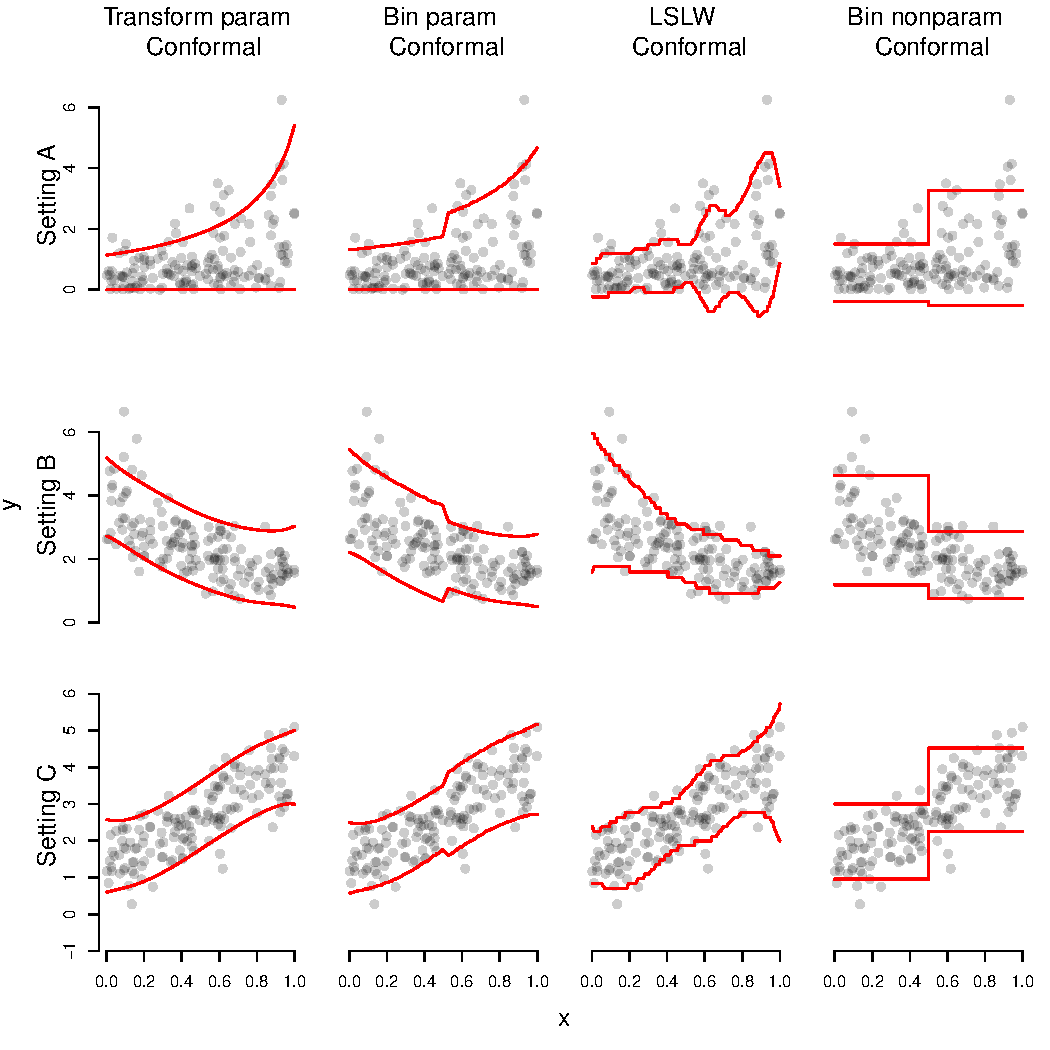
\includegraphics[width=\maxwidth]{figure/conformal-plots-1} 

\end{knitrout}
\end{center}
\caption{The depiction of conformal prediction regions when $n = 150$ that 
  appears in \citet{eck2019conformal}.  The rows display conformal prediction 
  regions across simulation settings.  The columns display the different 
  conformal prediction regions.  The top, middle, and bottom rows correspond 
  to simulation setting A with shape parameter equal to 1, simulation setting 
  B with shape parameter equal to 10, and simulation setting C respectively.  
  The first column displays the transformation parametric conformal prediction 
  region which is misspecified in row 2, the second column displays the binned 
  parametric conformal prediction region which is misspecified in row 2,
  the third column displays the least squares locally weighted conformal 
  prediction region, the fourth column displays the binned 
  nonparametric conformal prediction region.}
\label{conformal-plots}
\end{figure}



\newpage
\subsection{Plots corresponding to Section~\ref{sec:Gamma}}
\label{sec:gammaplots}

%Plot of conformal prediction regions in sim setting A when n = 150
\begin{figure}[h!]
\begin{center}
\begin{knitrout}
\definecolor{shadecolor}{rgb}{0.969, 0.969, 0.969}\color{fgcolor}
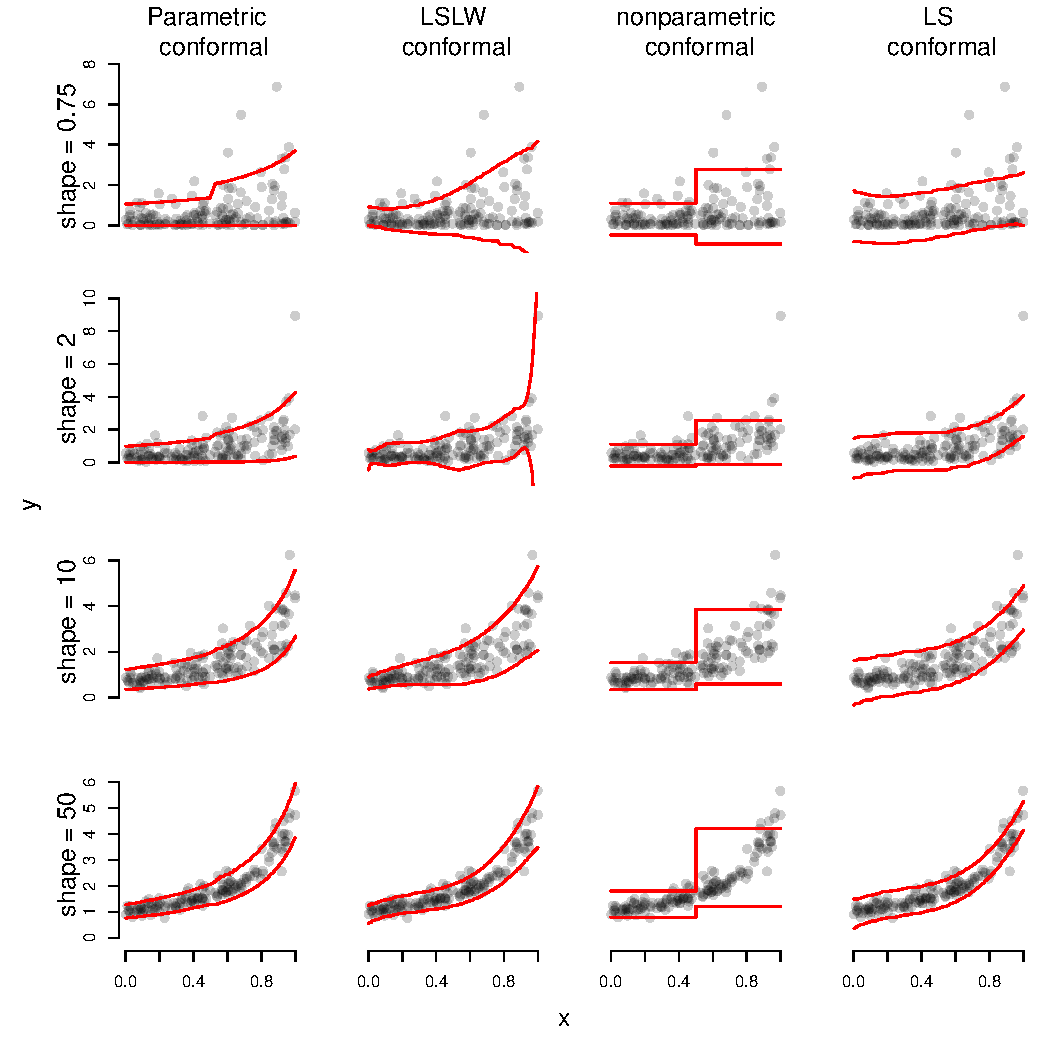
\includegraphics[width=\maxwidth]{figure/conformal-plots-A-150-1} 

\end{knitrout}
\end{center}
\caption{The depiction of conformal prediction regions under simulation 
  setting A when $n = 150$ and the number of bins equals 2.
}
\label{conformal-plots-A-150}
\end{figure}




\newpage
%Plot of conformal prediction regions in sim setting A when n = 250
\begin{figure}[h!]
\begin{center}
\begin{knitrout}
\definecolor{shadecolor}{rgb}{0.969, 0.969, 0.969}\color{fgcolor}
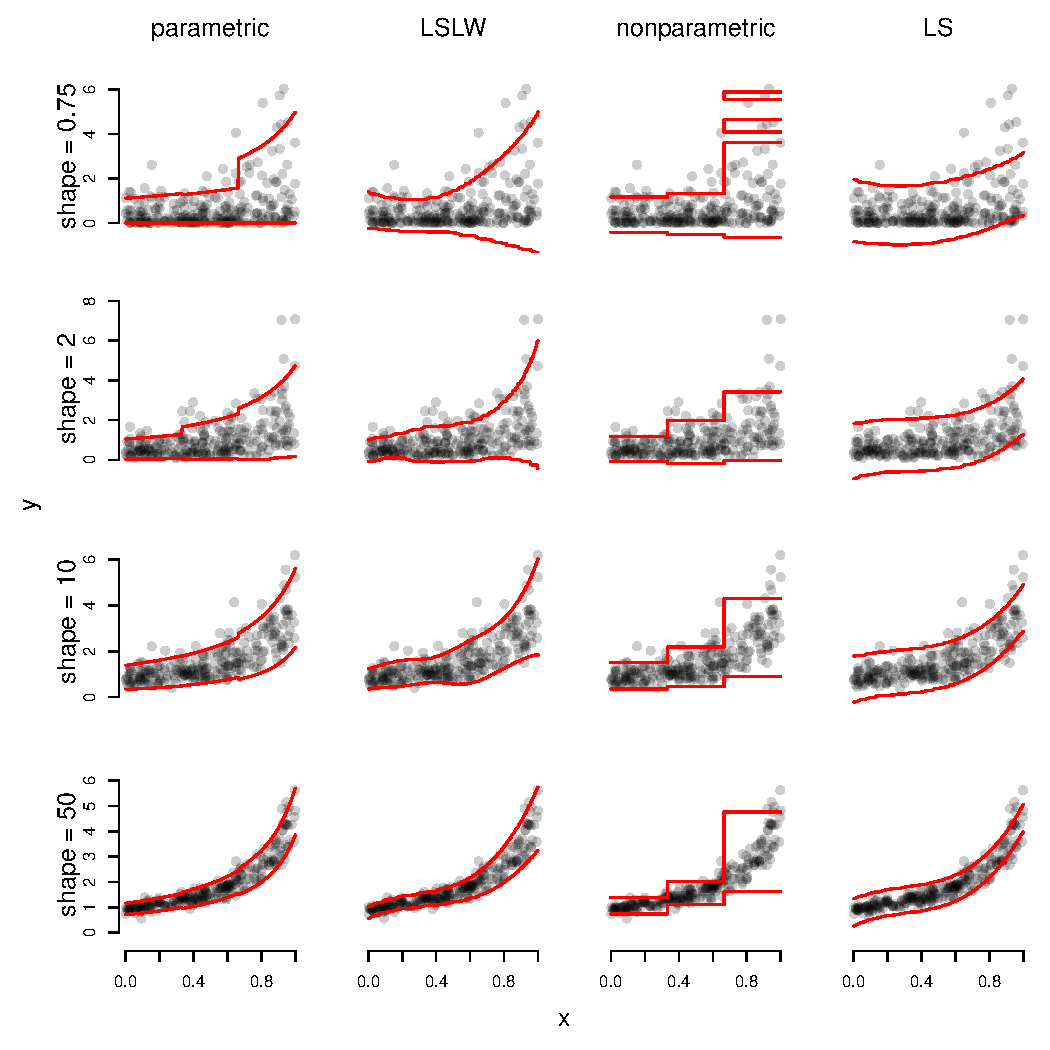
\includegraphics[width=\maxwidth]{figure/conformal-plots-A-250-1} 

\end{knitrout}
\end{center}
\caption{The depiction of conformal prediction regions under simulation 
  setting A when $n = 250$ and the number of bins equals 3.
}
\label{conformal-plots-A-250}
\end{figure}




\newpage
%Plot of conformal prediction regions in sim setting A when n = 500
\begin{figure}[h!]
\begin{center}
\begin{knitrout}
\definecolor{shadecolor}{rgb}{0.969, 0.969, 0.969}\color{fgcolor}
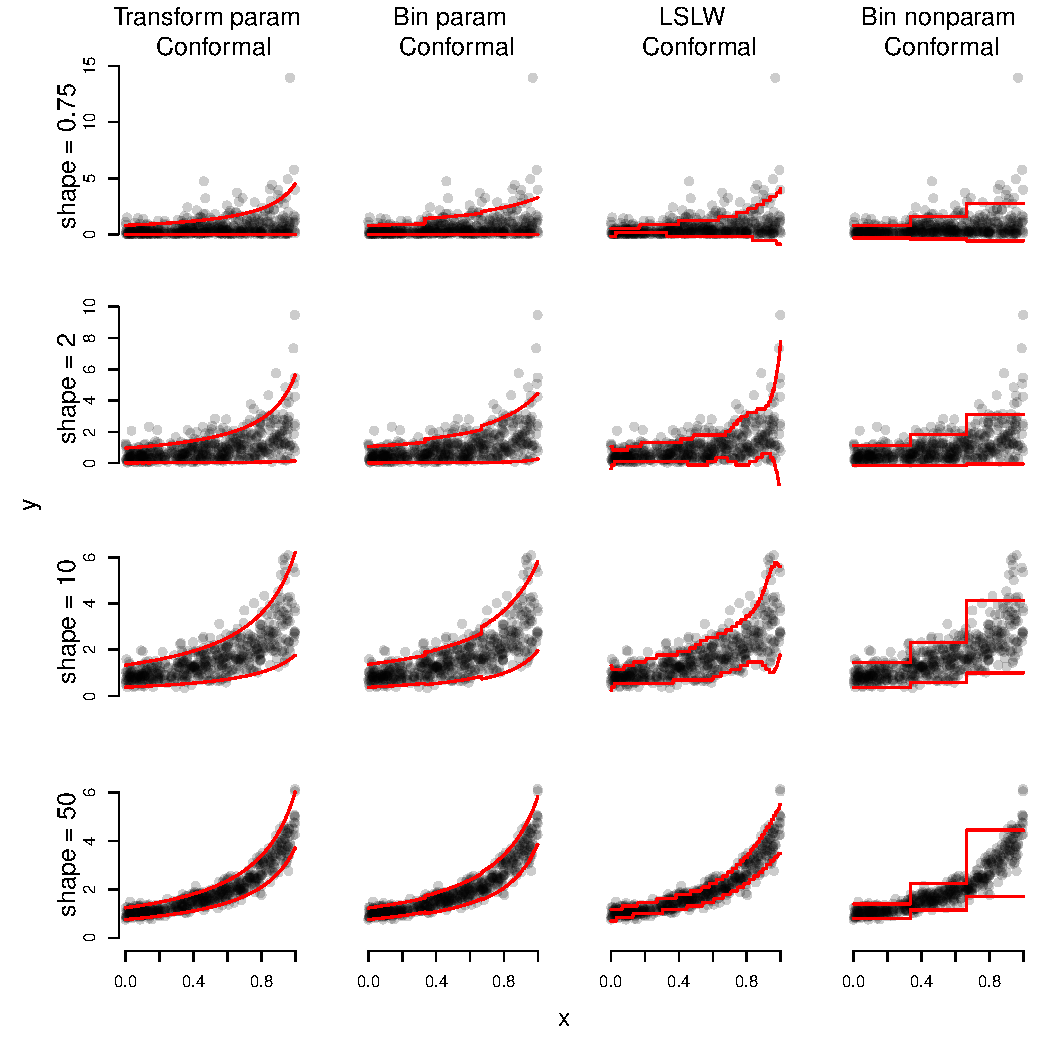
\includegraphics[width=\maxwidth]{figure/conformal-plots-A-500-1} 

\end{knitrout}
\end{center}
\caption{The depiction of conformal prediction regions under simulation 
  setting A when $n = 500$ and the number of bins equals 3.
}
\label{conformal-plots-A-500}
\end{figure}



\newpage
\subsection{Plots corresponding to Section~\ref{sec:misspec}}
\label{sec:misspecplots}


%Plot of conformal prediction regions in sim setting B when n = 150
\begin{figure}[h!]
\begin{center}
\begin{knitrout}
\definecolor{shadecolor}{rgb}{0.969, 0.969, 0.969}\color{fgcolor}
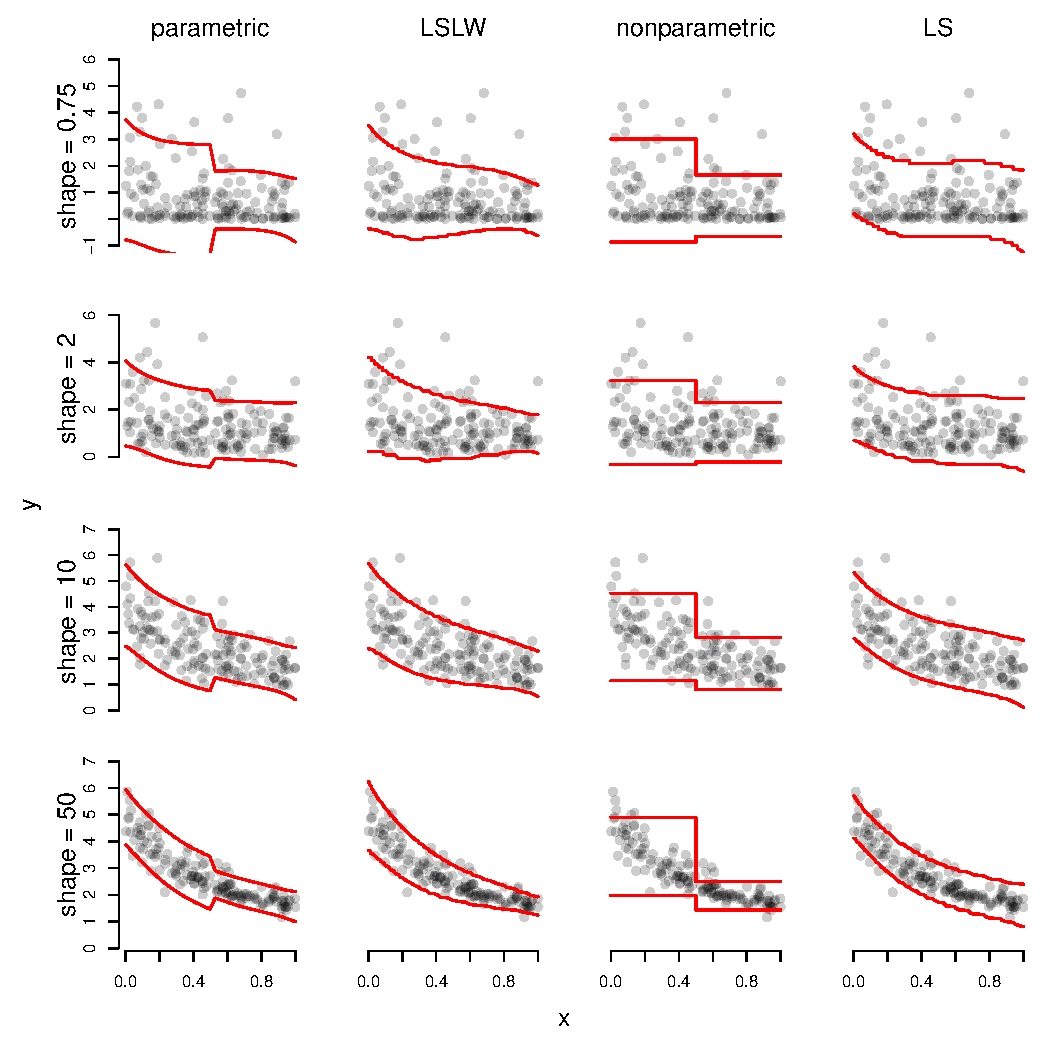
\includegraphics[width=\maxwidth]{figure/conformal-plots-B-150-1} 

\end{knitrout}
\end{center}
\caption{The depiction of conformal prediction regions under simulation 
  setting B when $n = 150$ and the number of bins equals 2.
}
\label{conformal-plots-B-150}
\end{figure}




\newpage
%Plot of conformal prediction regions in sim setting B when n = 250
\begin{figure}[h!]
\begin{center}
\begin{knitrout}
\definecolor{shadecolor}{rgb}{0.969, 0.969, 0.969}\color{fgcolor}
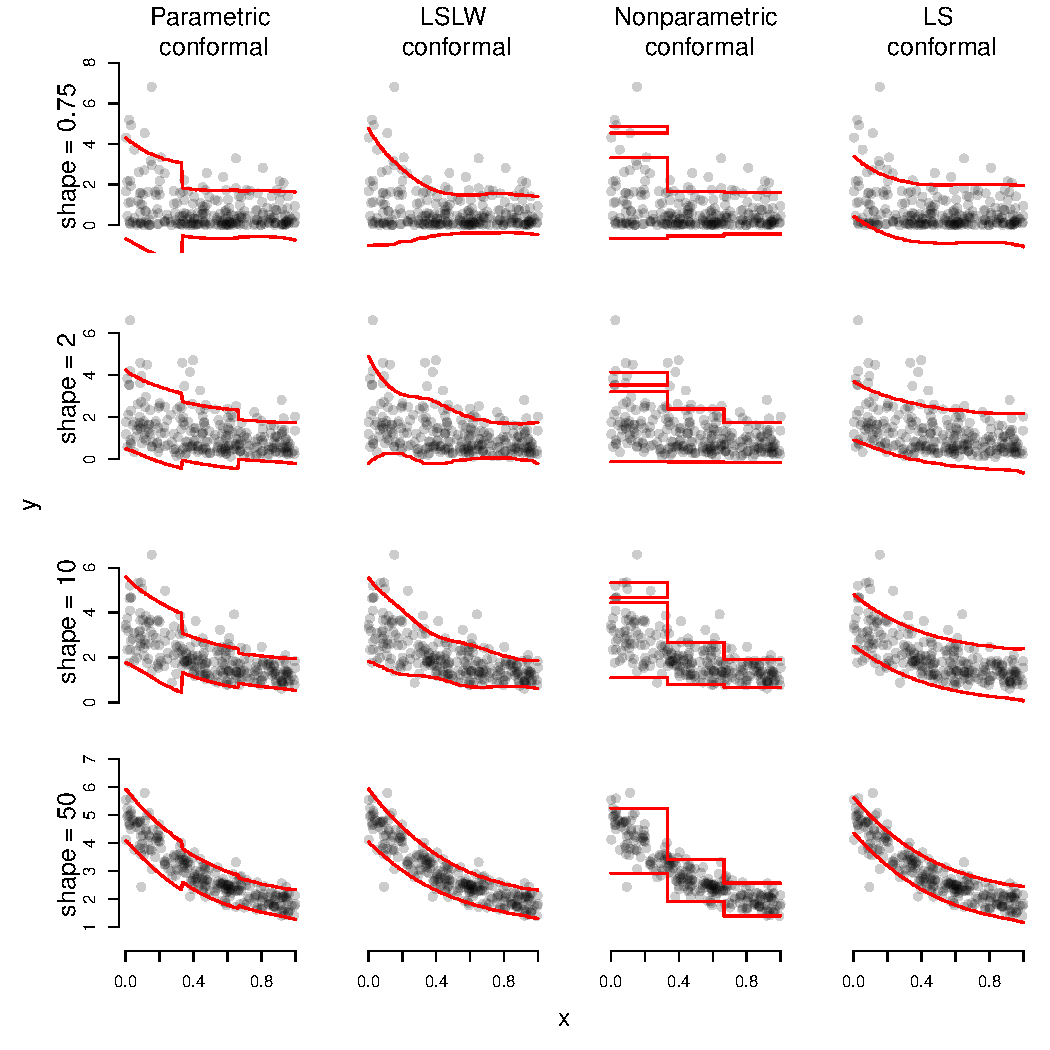
\includegraphics[width=\maxwidth]{figure/conformal-plots-B-250-1} 

\end{knitrout}
\end{center}
\caption{The depiction of conformal prediction regions under simulation 
  setting B when $n = 250$ and the number of bins equals 3.
}
\label{conformal-plots-B-250}
\end{figure}




\newpage
%Plot of conformal prediction regions in sim setting B when n = 500
\begin{figure}[h!]
\begin{center}
\begin{knitrout}
\definecolor{shadecolor}{rgb}{0.969, 0.969, 0.969}\color{fgcolor}
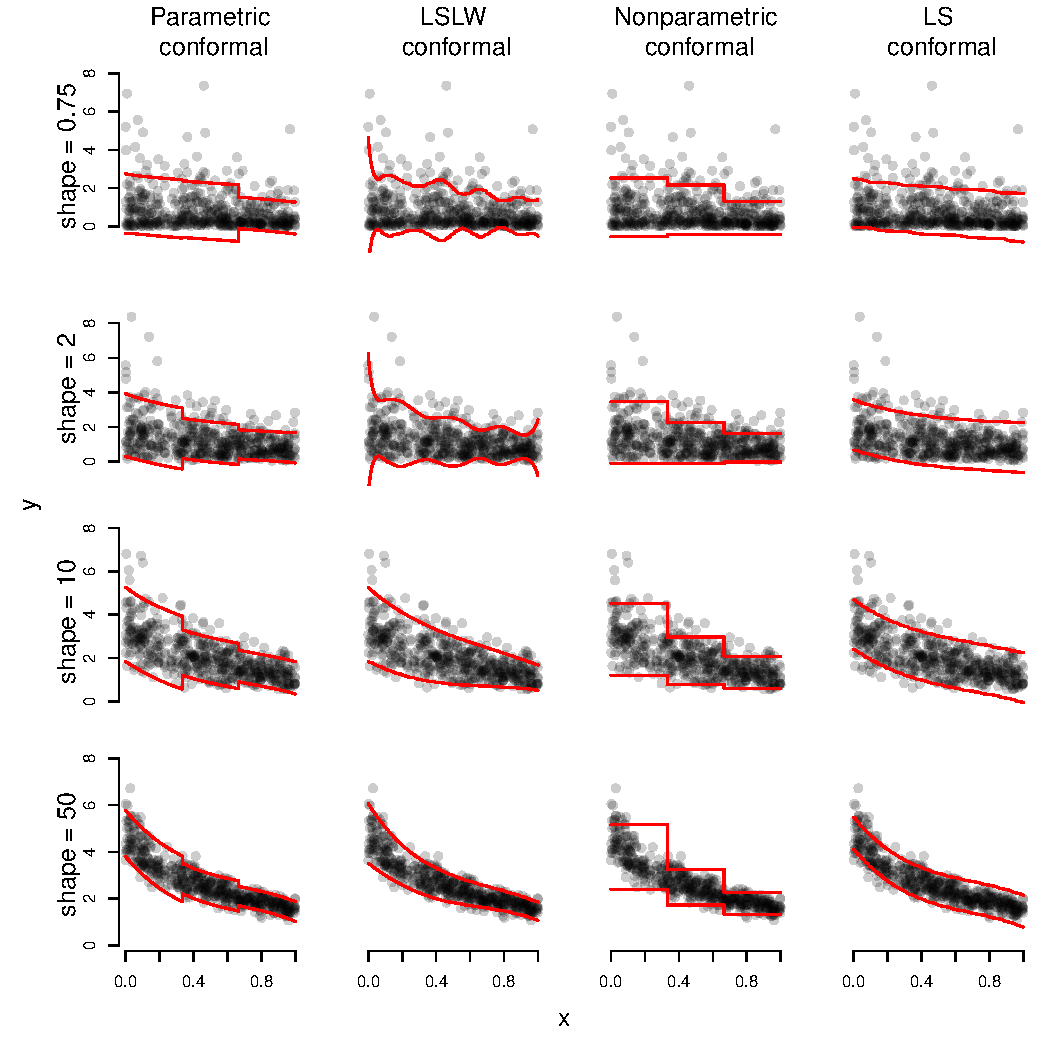
\includegraphics[width=\maxwidth]{figure/conformal-plots-B-500-1} 

\end{knitrout}
\end{center}
\caption{The depiction of conformal prediction regions under simulation 
  setting B when $n = 500$ and the number of bins equals 3.
}
\label{conformal-plots-B-500}
\end{figure}







\newpage
\subsection{Plots corresponding to Section~\ref{sec:regression}}
\label{sec:regressionplots}

%Plot of conformal prediction regions in sim setting C
\begin{figure}[h!]
\begin{center}
\begin{knitrout}
\definecolor{shadecolor}{rgb}{0.969, 0.969, 0.969}\color{fgcolor}
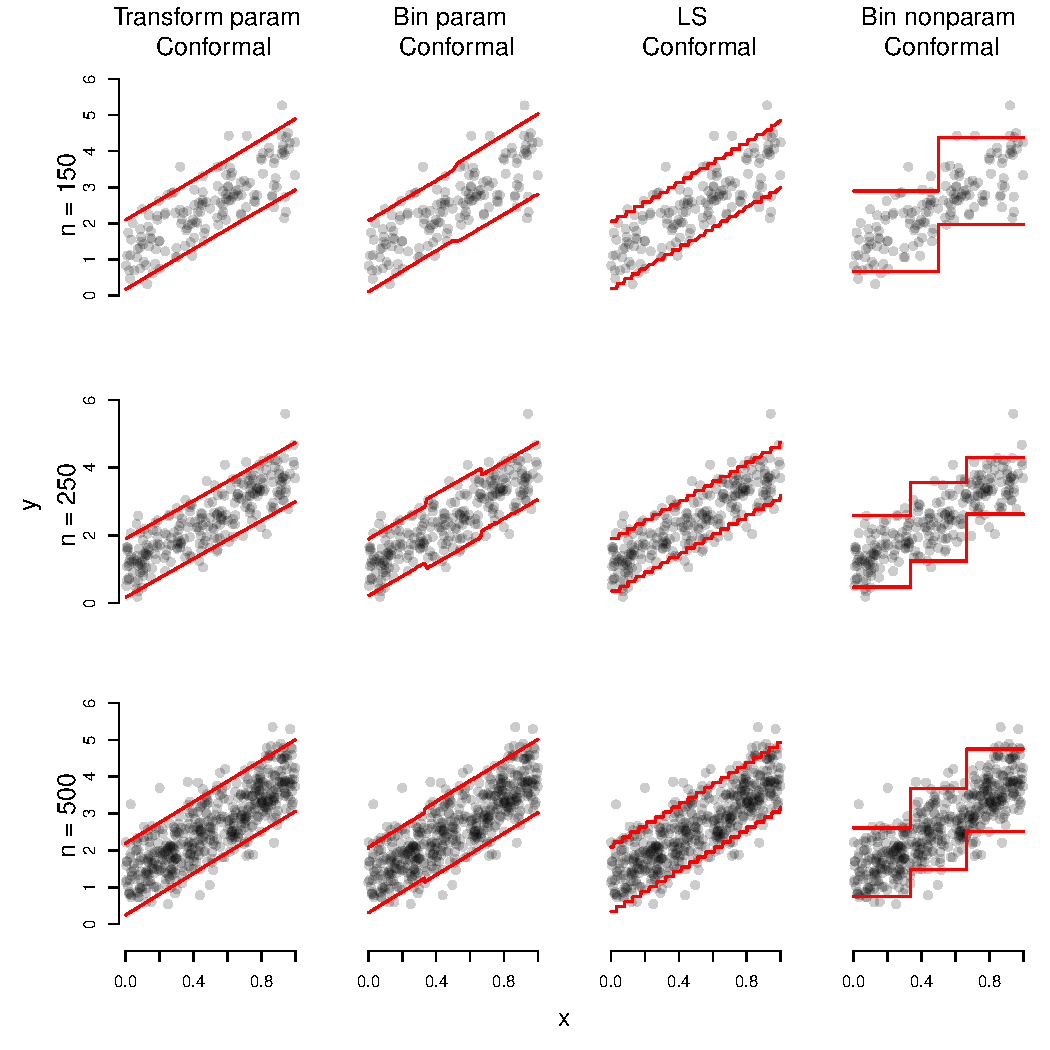
\includegraphics[width=\maxwidth]{figure/conformal-plots-C-1} 

\end{knitrout}
\end{center}
\caption{The depiction of conformal prediction regions under simulation 
  setting C.
}
\label{conformal-plots-C}
\end{figure}




\section{Creating this Document}
The purpose of this document is to provide a completely reproducible 
exploration and motivation of conformal prediction. All of the R code 
presented in this document (or the corresponding .Rnw file) is run when 
this document is compiled using the linux terminal.

This document is created from its source file 
\texttt{supplement-conformal.Rnw} using \texttt{knitr} and the 
\texttt{pdflatex} command in the linux terminal. The \texttt{knitr} R package 
needs to be installed before this document can be compiled. Open R and install 
this package if you have not previously done so. To compile this document in 
the linux terminal, enter the command 
\vspace{0.25cm}\\
\texttt{Rscript -e "library(knitr); knit('supplement-conformal.Rnw')"} 
\vspace{0.25cm}\\
This produces the LaTex .tex file with the name 
\texttt{supplement-conformal.tex}. To get a corresponding .pdf file, enter 
the command
\vspace{0.25cm}\\
\texttt{pdflatex supplement-conformal.tex} 
\vspace{0.25cm}\\
You may want to run the previous command twice in order to get labels and 
references right.

\bibliographystyle{plainnat}

\bibliography{conformalsources}

\end{document}

